% !TeX encoding = ISO-8859-1
% !TeX program = pdfLaTeX

%
% Dopo aver compilato il documento con LATEX ed aver eseguito BibTEX, � necessario compilare
% altre tre volte con LATEX: con l'ultima compilazione vengono inclusi nel documento i riferimenti
% finali, generati da backref.
%


\RequirePackage{ifpdf}
\ifpdf
 \documentclass[pdftex,11pt,a4paper,twoside,openright]{book}
\else
 \documentclass[11pt,a4paper,twoside,openright]{book}
\fi


%%%%%%%%%%%%%%%%%%%%%%%%%%%%%%%%%%%%%%%%%%%%%%%%%%%%%%%%%%%%%%%%%%%%%%%%%%%%%%%%%%%%%%%%%%%%%%%%%%%%
% Inclusioni di pacchetti

\usepackage{ifthen}
\usepackage[a4paper,top=3.5cm,bottom=3cm,left=2.2cm,right=4.3cm,bindingoffset=5mm]{geometry}
\usepackage[italian]{babel}
\usepackage[latin1]{inputenc}
\usepackage[colorlinks,hyperindex,linkcolor=blue,plainpages=false,bookmarksopen,%
            pagebackref, % opzione necessaria per usare backref
            bookmarksopenlevel=1,bookmarksnumbered,pdfstartview={XYZ null null 1.0}]{hyperref}
\usepackage[hyperpageref]{backref}
\usepackage{graphicx}
\usepackage{fancyhdr}
\usepackage[font=small,format=hang,labelfont={sl}]{caption}
\usepackage{subfig}
\usepackage{amsmath,amsthm}
% Per la \deltaup:
\usepackage{pxfonts}
% pxfonts ridefinisce tutti i font, del testo e matematici.
% ripristino alcuni caratteri matematici (come \triangleq):
\usepackage{amssymb,amsfonts}
% Ripristino i font a quelli originari, che pxfonts aveva ridefinito:
\usepackage{lmodern}
% titlesec serve a poter ridefinire il formato dei titoli di sezione e capitolo (\titleformat)
\usepackage[bf]{titlesec}
% Pacchetti per simboli e ambienti specifici:
\usepackage{extarrows}
\usepackage{textcomp}
\usepackage{array}
% PSTricks:
\usepackage{pstricks}
\usepackage{pst-math,pst-2dplot,pst-plot,pst-infixplot}
\usepackage{pst-pdf}
%\usepackage{pstricks-add}  % d� problemi perch� non riesce a trovare \pstScalePoint
\usepackage[italian,colorinlistoftodos,shadow]{todonotes}
\usepackage[smaller,printonlyused,withpage]{acronym}
% etex modifies the register allocation mechanism (per evitare errori con booktabs)
\usepackage{etex}
% booktabs serve per \toprule, \midrule e \bottomrule
\usepackage{booktabs}
% il pacchetto seguente serve perch� in alcuni casi (sperimentati) le note a margine compaiono nel margine sbagliato
\usepackage{mparhack}
%\usepackage{makeidx}
% Serve a eliminare le intestazioni delle pagine con contenuto vuoto (dopo ad esempio i capitoli)
% in modo che le pagine siano completamente vuote (anzich� avere la sola inestetica intestazione):
\usepackage{emptypage}
% per le appendici in ciascuna parte
\usepackage{appendix}
\usepackage[square,numbers]{natbib}
\usepackage{units}
\ifpdf
 \usepackage[protrusion=true,expansion=true]{microtype}
\fi


%%%%%%%%%%%%%%%%%%%%%%%%%%%%%%%%%%%%%%%%%%%%%%%%%%%%%%%%%%%%%%%%%%%%%%%%%%%%%%%%%%%%%%%%%%%%%%%%%%%%
% Informazioni sul documento

\title{\scshape{Appunti per il corso di\\\vspace{10pt} \Huge Comunicazioni numeriche}}
\author{\small Son Cafoni Trita Carni Emo Craccati\qquad\\\small\vspace{5pt}\qquad\dots non mi scocciare Foca Tritranciata!}
% Impostazioni per il pacchetto hyperref (per l'output in pdf):
\hypersetup{pdftitle={Appunti per il corso di Comunicazioni numeriche},%
            pdfsubject={Tratti dalle lezioni del prof. M. Martorella, Universit� di Pisa},%
            pdfauthor={Antonio Macr� ('Miro a Incanto'), Francesco Racciatti ('Strano Tic Cerca Fica')}}
\date{13 novembre 2009}


%%%%%%%%%%%%%%%%%%%%%%%%%%%%%%%%%%%%%%%%%%%%%%%%%%%%%%%%%%%%%%%%%%%%%%%%%%%%%%%%%%%%%%%%%%%%%%%%%%%%
% Impostazioni generali

% La riga seguente deve precedere i comandi che ridefiniscono intestazioni e pi� di pagina
% utilizzando il pacchetto fancyhdr (fancyhead, fancyhf...)
\pagestyle{fancy}
% Spazio normale dopo il punto fermo:
\frenchspacing
% L'opzione seguente serve ad evitare che, avendo ridefinito gli header in cui ci metto una riga
% orizzontale e un po' di spazi verticali, siano emessi innumerevoli warning perch� non stanno
% nelle dimensioni di default dell'header
\setlength{\headheight}{13.6pt}
% altrimenti le note a margine escono fuori la pagina
\setlength{\marginparwidth}{83pt}
% stile della bibliografia
\bibliographystyle{plain_ita}

\allowdisplaybreaks


%%%%%%%%%%%%%%%%%%%%%%%%%%%%%%%%%%%%%%%%%%%%%%%%%%%%%%%%%%%%%%%%%%%%%%%%%%%%%%%%%%%%%%%%%%%%%%%%%%%%
% Definizioni e ridefinizioni di comandi e ambienti

\newcommand{\textop}[1]{\textsl{#1}}
% Gestione TODO e commenti a margine:
\newcommand{\margincomment}[1]{\marginpar[\raggedleft\textsl{\footnotesize #1}]{\raggedright\textsl{\footnotesize #1}}}
\setlength{\marginparpush}{10pt}
\newcommand{\annotation}[3][]{\todo[size=\small,#1]{#3}\textcolor{orange}{#2}}
% Ridefinisco lo stile della pagina plain, ossia quello della prima pagina dei capitoli,
% (di default contiene il numero di pagina in basso al centro, lo elimino):
\fancypagestyle{plain}{\fancyhf{}\renewcommand{\headrulewidth}{0pt}}
% Ridefinisco le intestazioni per lo stile fancy (gi� impostato con \pagestyle{fancy})
\fancyhf{}
\fancyhead[LE,RO]{\thepage}
\fancyhead[LO]{\scshape\nouppercase{\rightmark}}
\fancyhead[RE]{\scshape\nouppercase{\leftmark}}
% Con le due righe seguenti modifico solamente lo spazio: ->\ \,<- anzich� \qquad
\renewcommand{\chaptermark}[1]{\markboth{\chaptername\ \thechapter.\ \,#1}{}}%
\renewcommand{\sectionmark}[1]{\markright{\thesection.\ \,#1}{}}
% Ridefinisco lo stile di parti, capitoli, sezioni e sottosezioni
\titleformat{\part}[display]{\centering\scshape}{\large\partname\ \thepart}{20pt}{\Huge}
\titleformat*{\chapter}{\titlerule[1pt]\vspace{2pt}\titlerule\vspace{2pt}\scshape}
\titleformat*{\section}{\Large\scshape}
\titleformat*{\subsection}{\large\scshape}
% Ridefinisco lo stile dei paragrafi (vedi anche to-proof)
\renewcommand{\paragraph}[1]{\bigskip\par\noindent\textsc{#1}\ \,}
\newtheoremstyle{teorema}
  {\bigskipamount}%      Space above, empty = `usual value'
  {3pt}%      Space below
  {\slshape}% Body font
  {}%         Indent amount (empty = no indent, \parindent = para indent)
  {\scshape}% Thm head font
  {.}%        Punctuation after thm head
  {1em}%     Space after thm head: " " = normal interword space;
        %       \newline = linebreak
  {}%         Thm head spec (can be left empty, meaning `normal')
\theoremstyle{teorema}
\newtheorem{teorema}{Teorema}[chapter]
\newtheorem{proprieta}{Propriet�}[chapter]
\newtheorem{proposizione}[teorema]{Proposizione}
\newtheorem{lemma}[teorema]{Lemma}
\newtheoremstyle{definizione}{\medskipamount}{\medskipamount}{\slshape}{}{\scshape}{:}{.5em}{}
\theoremstyle{definizione}
\newtheorem{definizione}{Definizione}[chapter]
\newtheorem{criterio}[definizione]{Criterio}
\newtheorem{condizione}[definizione]{Condizione}
\newtheoremstyle{esempio}{\bigskipamount}{3pt}{}{}{\scshape}{.}{.5em}{}
\theoremstyle{esempio}
\newtheorem{esempio}{Esempio}[chapter]
% Ridefinisco il simbolo da mettere alla fine delle dimostrazioni:
\renewcommand{\qedsymbol}{$\square$}
% Immagini inglobabili nel pdf (tramite \includegraphics):
\DeclareGraphicsExtensions{.pdf,.png,.jpg}
% Il percorso dove sono contenute le immagini:
\graphicspath{{./img/}}
% Definizione di operatori matematici:
\DeclareMathOperator{\sgn}{sgn}
\DeclareMathOperator{\sinc}{sinc}
%\DeclareMathOperator{\TCF}{\mathcal{T\mspace{-1.5mu}C\mspace{-0.5mu}F}}
%\DeclareMathOperator{\ATCF}{\mathcal{AT\mspace{-1.5mu}C\mspace{-0.5mu}F}}
%\DeclareMathOperator{\TSF}{\mathcal{TSF}}
%\DeclareMathOperator{\ATSF}{\mathcal{ATSF}}
%\DeclareMathOperator{\TFS}{\mathcal{T\mspace{-1.5mu}F\mspace{-0.5mu}S}}
%\DeclareMathOperator{\ATFS}{\mathcal{AT\mspace{-1.5mu}F\mspace{-0.5mu}S}}
\DeclareMathOperator{\TCF}{\mathrm{TCF}}
\DeclareMathOperator{\ATCF}{\mathrm{TCF^{-1}}}
\DeclareMathOperator{\TSF}{\mathrm{TSF}}
\DeclareMathOperator{\ATSF}{\mathrm{TSF^{-1}}}
\DeclareMathOperator{\TFS}{\mathrm{TFS}}
\DeclareMathOperator{\ATFS}{\mathrm{TFS^{-1}}}
\DeclareMathOperator{\T}{\mathcal{T}}
\DeclareMathOperator{\E}{E}
% Altri operatori:
\newcommand{\rect}[3][]{\operatorname{rect}\!\left(#1\dfrac{#2}{#3}\right)}
\newcommand{\vrect}{\operatorname{rect}}
\newcommand{\gp}[1]{_\textrm{\textsmaller{#1}}}
\renewcommand{\Re}{\mathop{}\!\mathbf{Re}}
\renewcommand{\Im}{\mathop{}\!\mathbf{Im}}
\renewcommand{\Pr}{\operatorname{Pr}}
\let\olddelta\delta
\renewcommand{\delta}{\mathop{}\!\deltaup}
\renewcommand{\epsilon}{\varepsilon}
\renewcommand{\theta}{\vartheta}
%\renewcommand{\pi}{\piup}
\newcommand{\ud}{\mathop{}\!\mathrm{d}}
\newcommand{\dB}{\mathop{}\!\mathrm{dB}}
\renewcommand*{\j}{\mathrm{j}}
\newcommand{\abs}[1]{\left\lvert#1\right\rvert}
\newcommand{\N}{\mathbb{N}}
\newcommand{\R}{\mathbb{R}}
\newcommand{\Z}{\mathbb{Z}}
\newcommand{\C}{\mathbb{C}}
% Non proprio ortodosse:
\newcommand{\e}{\mathop{}\!\mathrm{e}}
\let\oldu\u\renewcommand{\u}{\mathop{}\!\mathrm{u}}
% Ridefinisco la \sqrt in modo che abbia una lineetta che "richiude" l'argomento:
\let\oldsqrt\sqrt
\def\sqrt{\mathpalette\DHLhksqrt}\def\DHLhksqrt#1#2{%
\setbox0=\hbox{$#1\oldsqrt{#2\,}$}\dimen0=\ht0\advance\dimen0-0.2\ht0
\setbox2=\hbox{\vrule height\ht0 depth -\dimen0}{\box0\lower0.4pt\box2}}
% affinch� la bibliografia sia una section della prefazione e non un capitolo a parte
\renewcommand{\bibsection}{\section*{\bibname}}
% per backref
\renewcommand{\backref}[1]{}
% per avere in backref i riferimenti in italiano anzich� in inglese
\renewcommand*{\backreftwosep}{ e~}
\renewcommand*{\backreflastsep}{ e~}
\renewcommand*{\backrefalt}[4]{\ifcase #1\relax\or(Citato a pagina~#2.)\else(Citato alle pagine~#2.)\fi}


%%%%%%%%%%%%%%%%%%%%%%%%%%%%%%%%%%%%%%%%%%%%%%%%%%%%%%%%%%%%%%%%%%%%%%%%%%%%%%%%%%%%%%%%%%%%%%%%%%%%
% Corpo del documento

\begin{document}

\frontmatter
\pagenumbering{Roman}
\maketitle

\thispagestyle{empty}
\null\vspace{\stretch{1}}
\phantomsection
\pdfbookmark[0]{Contributi}{contributors}
\section*{Hanno contribuito}
\begin{description}
\item[Antonio Macr�] Ha scritto i capitoli~\ref{cha:segnali}, \ref{cha:segnali-periodici}, \ref{cha:segnali-aperiodici}, \ref{cha:sistemi-lineari}, \ref{cha:sistemi-non-lineari}, \ref{cha:segnali-campionati}, \ref{cha:processi-stocastici}.
\item[Francesco Racciatti] Ha contribuito per il capitolo~\ref{cha:segnali-aperiodici}.
\end{description}



\cleardoublepage
\phantomsection
\pdfbookmark[0]{\contentsname}{contents}
{\small\tableofcontents}

% !TeX encoding = ISO-8859-1
% !TeX root = appunti.tex

\chapter{Prefazione}

\markboth{Prefazione}{Prefazione}

Questi Appunti nascono per esser la materia di una forma che si chiama \LaTeX. Il loro scopo iniziale era fornire sostanza per un tempo e un esercizio appena sufficienti per consentire al sottoscritto di cominciare a usare questo strumento nel modo pi� efficace e pulito possibile.

Per quanto riguarda la prima parte, i capitoli~\ref{cha:segnali}, \ref{cha:sistemi-lineari}, \ref{cha:sistemi-non-lineari}, \ref{cha:segnali-campionati} sono stati scritti a partire dalle lezioni del professor Martorella integrando successivamente dal~\citep{b:luise}. I capitoli~\ref{cha:segnali-periodici}, \ref{cha:segnali-aperiodici} sono stati invece ottenuti principalmente rielaborando il contenuto del libro, ignorando parti non utili ai fini del nostro corso e in ogni caso avendo come guida il programma svolto a lezione dal prof.~Martorella.

La seconda parte di questi Appunti � stata ottenuta partendo dalle lezioni del prof.~Berizzi e dal materiale che lo stesso ha messo in rete. Tuttavia, ampio spazio � stato dato a integrazioni dal~\citep{b:luise} (per il capitolo~\ref{cha:processi-stocastici}) e dal~\citep{b:Dandrea} (per i restanti capitoli della seconda parte), nell'ottica di fornire un fondamentale impianto teorico agli argomenti trattati (totalmente assente nelle slide del professore).

Le \annotation[nolist]{annotazioni a margine}{Come questa!} indicano parti del testo che sarebbe meglio rivedere, o perch� possono contenere imprecisioni o perch� il contenuto non � espresso nel migliore dei modi. I capitoli e le sezioni contrassegnati con \textbf{un asterisco (*)} sono opzionali: il professore (Martorella o Berizzi) non li ha trattati esplicitamente a lezione. Infine, i capitoli e le sezioni contrassegnati con \textbf{due asterischi (**)} sono solamente delle bozze.


\vspace{\stretch{1}}
\begin{flushright}
Antonio Macr�\\
\vspace{1pt}
9 luglio 2009 --- 13 novembre 2009
\end{flushright}
\vspace{\stretch{4}}


\phantomsection
\pdfbookmark[0]{Nota ai posteri}{note}
\section*{Nota ai posteri}

Avendo finalmente passato l'esame (12 novembre 2009), non metter� pi� mano a questi Appunti. Due note a chi vorr� continuare il lavoro.

Vanno convertite in \LaTeX{} (con PSTricks) alcune immagini, come la figura a pagina~\pageref{fig:sistema-di-elaborazione-e-trasmissione} e le varie figure nel paragrafo~\ref{sec:relazione-tcf-tsf-e-formule-di-poisson} (da pag.~\pageref{sec:relazione-tcf-tsf-e-formule-di-poisson}).
Andrebbero approfonditi argomenti come l'autocorrelazione di segnali periodici (la sua \acsfont{TCF} � la \acsfont{DSP}?), il filtraggio di segnali campionati. Va riaggiustato l'appendice~\ref{cha:numeri-complessi}. Inoltre, potrebbe essere utile un'ulteriore operazione di \emph{refactoring} per il capitolo~\ref{cha:processi-stocastici}: nel paragrafo~\ref{sec:relazione-io-tra-le-statistiche} forse � possibile togliere qualcosa e scremare un po'; che fare (pagina~\pageref{sec:densita-spettrale-di-un-processo-ssl}) della \emph{densit� spettrale di potenza di un processo stazionario}? Il prof.~non ha detto praticamente nulla sui processi parametrici, che c'� da dire? Infine, gli altri capitoli della seconda parte sono sostanzialmente ancora delle bozze.


\clearpage

\markboth{Acronimi, Annotazioni e Bibliografia}{Acronimi, Annotazioni e Bibliografia}

\phantomsection
\pdfbookmark[0]{Acronimi}{acronimi}
\section*{Acronimi}
\begin{acronym}[ATCF]
\acro{TSF}{\textit{Trasformata Serie Di Fourier}}
\acro{ATSF}{\textit{Antitrasformata Serie Di Fourier}}
\acro{TCF}{\textit{Trasformata Continua Di Fourier}}
\acro{ATCF}{\textit{Antitrasformata Continua Di Fourier}}
\acro{SLS}{\textit{Sistemi Lineari Stazionari}}
\acro{BIBO}{\textit{Bounded Input Bounded Output}}
\acro{TFS}{\textit{Trasformata Di Fourier di una Sequenza}}
\acro{SSS}{\textit{Stazionario in Senso Stretto}}
\acro{SSL}{\textit{Stazionario in Senso Lato}}
\acro{PAM}{\textit{Pulse Amplitude Modulation}}
\acro{ISI}{\textit{InterSymbol Interference}}
\end{acronym}

\pdfbookmark[0]{Annotazioni}{annotazioni}
\listoftodos[Annotazioni]

\pdfbookmark[0]{\bibname}{bibliografia}
{\nocite{*}\small\bibliography{bibliografia}}


\mainmatter

\part{Segnali deterministici}
% !TeX encoding = ISO-8859-1
% !TeX root = appunti.tex

\chapter{Segnali}
\label{cha:segnali}


\section{Concetti generali}

Un \emph{segnale} � una rappresentazione di una grandezza fisica a cui � associata informazione. Per esempio, un segnale audio o video, un elettrocardiogramma, l'uscita di un sensore di temperatura, umidit� o pressione. Il segnale � quindi diverso dalla grandezza fisica rappresentata, rispetto alla quale ne � una astrazione, una rappresentazione in forma (spesso) matematica, utile a studiare e caratterizzare determinate propriet� del segnale stesso e poterlo elaborare.

\paragraph{Classificazione dei segnali.}
Una prima classificazione dei segnali � tra i segnali deterministici e quelli aleatori:
\begin{itemize}
\item \emph{determinati} o \emph{deterministici}, dei quali si conosce con esattezza il valore che assumono a un certo istante (in quanto rappresentati mediante una funzione analitica o un grafico);
\item \emph{aleatori}, dei quali non si pu� conoscere \emph{a priori} il valore assunto a determinati istanti, ma si ha solamente una conoscenza di massima tramite dati statistici e alcune propriet�, motivo per cui possono essere rappresentati come un \emph{insieme} di segnali.%
\footnote{L'\emph{alea} � il grado di indeterminazione relativo alla conoscenza di questi segnali.}
\end{itemize}

\paragraph{Dimensionalit�.}
Un elettrocardiogramma o un sensore di temperatura forniscono segnali scalari, ma altri segnali possono avere dimensionalit� maggiore, per esempio un segnale audio stereo, con i canali destro e sinistro. Peraltro, non solo il segnale pu� essere multidimensionale, ma anche la sua variabile indipendente. In generale un segnale � una funzione:
%
\[v(x)\colon \R^{n}\to\R^{n}.\]
%
Un esempio di segnale con variabile indipendente multidimensionale � un $x(t_1,t_2)$ con $(t_1,t_2)$ coordinate su uno schermo e $x(t_1,t_2)$ che rappresenta il livello di grigio del relativo pixel (televisione in bianco e nero).

Noi analizzeremo principalmente segnali (scalari ma) complessi di variabile reale.

\paragraph{Esempi.}
Ecco alcuni esempi di segnali:
%
\begin{itemize}
\item \emph{elettrocardiogramma} $x(t)$, dove $t$ � il tempo e $x$ l'ampiezza;
\item \emph{audio stereo} $\big(x(t),y(t)\big)$, dove $x$ e $y$ sono le ampiezza dei canali destro e sinistro;
\item \emph{immagine in B/N} $z(x,y)$, con $(x,y)$ coordinate spaziali e $z$ intensit� di grigio;
\item \emph{immagine a colori RBG} $z(x,y)$, dove $z=(z_1,z_2,z_3)$ � l'intensit� dei colori.
\end{itemize}

\paragraph{Tipologia di segnali.}
Un'altra suddivisione dei segnali pu� esser fatta a seconda delle caratteristiche della variabile indipendente e della variabile dipendente:
%
\begin{itemize}
\item \emph{segnali a tempo continuo} nei quali la variabile $t$ assume con continuit� tutti i valori reali
        contenuti in un certo intervallo (anche da $-\infty$ a $+\infty$):
        \[x(t),\quad y(t),\quad\ldots\]
\item \emph{segnali a tempo discreto} quando la variabile indipendente ($n$) assume solamente valori discreti:
        \[x[n],\quad y[n],\quad\ldots\]
\item \emph{segnali ad ampiezza continua} se la grandezza fisica del segnale assume con continuit� tutti i
        valori (reali o complessi) all'interno di un certo intervallo (anche illimitato);
\item \emph{segnali ad ampiezza discreta} nei quali la grandezza fisica del segnale assume solo valori
        discreti (reali o complessi) appartenenti a un certo alfabeto (il pi� semplice � un alfabeto binario).
\end{itemize}
\begin{center}
\begin{tabular}{>{\slshape}rcc}
\toprule
                  & \textsl{tempo continuo} & \textsl{tempo discreto} \\
\midrule
ampiezza continua & analogici               & sequenza \\
ampiezza discreta & quantizzati             & numerici \\
\bottomrule
\end{tabular}\\
\end{center}

Segnali analogici tipici sono: il segnale audio analogico, video analogico, elettrocardiogramma, eccetera.

I segnali tempo discreti ad ampiezza discreta sono le sequenze e i segnali campionati. Esiste una differenza tra i due. Le sequenze possono essere ottenute da sorgenti che sono intrinsecamente discrete, come ad esempio il risultato di una misura periodica della temperatura
%
\begin{center}\framebox{\begin{pspicture*}(-0.5,-0.6)(5,2)
  \psaxes[linewidth=0.4pt,labels=none,ticks=none]{->}(0,0)(-0.2,-0.3)(4.7,1.7)
  \psline[linewidth=0.5pt](0.6,0)(0.6,1.0)
  \psline[linewidth=0.5pt](1.4,0)(1.4,0.8)
  \psline[linewidth=0.5pt](2.2,0)(2.2,0.7)
  \psline[linewidth=0.5pt](2.8,0)(2.8,1.2)
  \psline[linewidth=0.5pt](3.8,0)(3.8,1.1)
  \pscircle*(0.6,1.0){1pt}
  \pscircle*(1.4,0.8){1pt}
  \pscircle*(2.2,0.7){1pt}
  \pscircle*(2.8,1.2){1pt}
  \pscircle*(3.8,1.1){1pt}
  \uput[u](0.6,0.9){$\scriptscriptstyle{20{,}3\text{\textcelsius}}$}
  \uput[u](1.4,0.7){$\scriptscriptstyle{16{,}5\text{\textcelsius}}$}
  \uput[u](2.2,0.6){$\scriptscriptstyle{14{,}1\text{\textcelsius}}$}
  \uput[u](2.8,1.1){$\scriptscriptstyle{24{,}9\text{\textcelsius}}$}
  \uput[u](3.8,1.0){$\scriptscriptstyle{22{,}7\text{\textcelsius}}$}
  \uput[d](4.6,0){$n$}
\end{pspicture*}}\end{center}
%
oppure per campionamento di segnali analogici:
%
\begin{center}\framebox{\begin{pspicture*}(-4.5,-1)(4.5,1.6)
  \psaxes[linewidth=0.5pt,labels=none,ticks=none]{->}(0,0)(-4.2,-0.7)(4.2,1.3)
  \uput[d](4.1,0){$t$}
  \psplot[linewidth=0.6pt,plotstyle=curve,plotpoints=200]% 0.5*sin(500*x) - 0.2*cos(300*x)
         {-3.7}{3.7}{0.5 x 100 mul sin mul 0.2 x 50 mul cos mul add}
  \psline[linewidth=0.5pt](-3.2,-0.05)(-3.2,0.05)
  \psline[linewidth=0.5pt,linestyle=dashed,dash=1pt 1pt](-3.2,0.1)(-3.2,0.14)
  \pscircle*(-3.2,0.14){1pt}
  \psline[linewidth=0.5pt](-2.4,-0.05)(-2.4,0.05)
  \psline[linewidth=0.5pt,linestyle=dashed,dash=1pt 1pt](-2.4,0.1)(-2.4,0.32)
  \pscircle*(-2.4,0.32){1pt}
  \psline[linewidth=0.5pt](-1.6,-0.05)(-1.6,0.05)
  \psline[linewidth=0.5pt,linestyle=dashed,dash=1pt 1pt](-1.6,-0.1)(-1.6,-0.15)
  \pscircle*(-1.6,-0.15){1pt}
  \psline[linewidth=0.5pt](-0.8,-0.05)(-0.8,0.05)
  \psline[linewidth=0.5pt,linestyle=dashed,dash=1pt 1pt](-0.8,-0.1)(-0.8,-0.33)
  \pscircle*(-0.8,-0.33){1pt}
  \pscircle*(0,0.21){1pt}
  \psline[linewidth=0.5pt](0.8,-0.05)(0.8,0.05)
  \psline[linewidth=0.5pt,linestyle=dashed,dash=1pt 1pt](0.8,0.1)(0.8,0.63)
  \pscircle*(0.8,0.63){1pt}
  \psline[linewidth=0.5pt](1.6,-0.05)(1.6,0.05)
  \psline[linewidth=0.5pt,linestyle=dashed,dash=1pt 1pt](1.6,0.1)(1.6,0.22)
  \pscircle*(1.6,0.22){1pt}
  \psline[linewidth=0.5pt](2.4,-0.05)(2.4,0.05)
  \psline[linewidth=0.5pt,linestyle=dashed,dash=1pt 1pt](2.4,-0.1)(2.4,-0.52)
  \pscircle*(2.4,-0.52){1pt}
  \psline[linewidth=0.5pt](3.2,-0.05)(3.2,0.05)
  \psline[linewidth=0.5pt,linestyle=dashed,dash=1pt 1pt](3.2,-0.1)(3.2,-0.5)
  \pscircle*(3.2,-0.5){1pt}
\end{pspicture*}}\end{center}

Per i segnali quantizzati la variabile indipendente � continua, mentre la variabile dipendente (l'ampiezza del
segnale) assume solo valori discreti, appartenenti a un certo alfabeto. Possono scaturire ad esempio da segnali
di led luminosi (acceso/spento, come per una comunicazione in codice Morse):
%
\begin{center}\framebox{\setlength{\unitlength}{1mm}
\begin{pspicture*}(-1,-0.6)(6,2)
  \psaxes[linewidth=0.4pt,labels=none,ticks=none]{->}(0,0)(-0.2,-0.3)(5.7,1.7)
  \psline[linewidth=1pt](0.3,0.4)(1.1,0.4)
  \psline[linewidth=0.5pt](1.1,0.4)(1.1,1.0)
  \psline[linewidth=1pt](1.1,1.0)(2.4,1.0)
  \psline[linewidth=0.5pt](2.4,1.0)(2.4,0.4)
  \psline[linewidth=1pt](2.4,0.4)(3.3,0.4)
  \psline[linewidth=0.5pt](3.3,0.4)(3.3,1.0)
  \psline[linewidth=1pt](3.3,1.0)(4.1,1.0)
  \psline[linewidth=0.5pt](4.1,1.0)(4.1,0.4)
  \psline[linewidth=1pt](4.1,0.4)(5.1,0.4)
  \psline[linewidth=0.5pt](5.1,0.4)(5.1,1.0)
  \psline[linewidth=1pt](5.1,1.0)(5.4,1.0)
  \uput[l](0,0.4){$\scriptscriptstyle{ON}$}
  \uput[l](0,1.0){$\scriptscriptstyle{OFF}$}
  \uput[d](5.6,0){$t$}
\end{pspicture*}}\end{center}

I segnali digitali (detti anche sequenze numeriche) hanno sia variabile indipendente che variabile dipendente
discreta, appartenente a un certo alfabeto (un insieme finito). Per questo motivo sono interamente
rappresentabili tramite bit, e si ottengono infatti tipicamente come conversione analogico-digitale per il
trattamento dell'informazione tramite calcolatori.
%
\begin{center}\framebox{\setlength{\unitlength}{1mm}\begin{tabular}{ccc}
\begin{pspicture*}(-1.8,-0.7)(2.1,1.6)
  \psaxes[linewidth=0.5pt,labels=none,ticks=none]{->}(0,0)(-1.7,-0.4)(1.9,1.4)
  \uput[d](1.8,0){$t$}
  \uput[l](0,1.2){$x(t)$}
  \psplot[linewidth=0.6pt,plotstyle=curve,plotpoints=200]%
         {-1.6}{1.7}{0.4 x 500 mul sin mul 0.2 x 400 mul cos mul add 0.4 add}
\end{pspicture*}&
\begin{pspicture*}(-1.8,-1.15)(1.9,1.15)
  \psframe[linewidth=0.5pt](-0.7,0.4)(0.7,-0.4)
  \uput[u](0,-0.4){A/D}
  \uput[u](-1.2,0){$\scriptstyle{x(t)}$}
  \uput[u](1.2,0){$\scriptstyle{d[n]}$}
  \psline[linewidth=0.5pt]{->}(-1.7,0)(-0.7,0)
  \psline[linewidth=0.5pt]{->}(0.7,0)(1.7,0)
\end{pspicture*}&
\begin{pspicture*}(-0.5,-0.5)(3.7,1.8)
  \psaxes[linewidth=0.4pt,labels=none,ticks=none]{->}(0,0)(-0.4,-0.3)(3.5,1.6)
  \uput[l](0,0.4){$\scriptstyle{0}$}
  \uput[l](0,1.0){$\scriptstyle{1}$}
  \uput[r](0,1.4){$d[n]$}
  \uput[d](3.4,0){$n$}
  \psline[linewidth=0.5pt](-0.05,0.4)(0.05,0.4)
  \psline[linewidth=0.5pt](-0.05,0.8)(0.05,0.8)
  \psline[linewidth=0.5pt](0.5,-0.05)(0.5,0.8)
  \pscircle*(0.5,0.8){1pt}
  \psline[linewidth=0.5pt](1.0,-0.05)(1.0,0.4)
  \pscircle*(1.0,0.4){1pt}
  \psline[linewidth=0.5pt](1.5,-0.05)(1.5,0.4)
  \pscircle*(1.5,0.4){1pt}
  \psline[linewidth=0.5pt](2.0,-0.05)(2.0,0.8)
  \pscircle*(2.0,0.8){1pt}
  \psline[linewidth=0.5pt](2.5,-0.05)(2.5,0.8)
  \pscircle*(2.5,0.8){1pt}
  \psline[linewidth=0.5pt](3.0,-0.05)(3.0,0.8)
  \pscircle*(3.0,0.8){1pt}
\end{pspicture*}\end{tabular}}\end{center}

Durante il corso capiremo come funziona un sistema di codifica e decodifica dell'informazione, e come
questa venga trasmessa, rendendola disponibile all'utente \textit{quasi} uguale a come era stata trasmessa.

Un esempio � la codifica, trasmissione e decodifica di un sistema audio. Innanzitutto, un microfono funge da trasduttore,%
\footnote{Un \emph{trasduttore} � un dispositivo che cambia la natura fisica del segnale senza alterarne la forma (e quindi l'informazione associata).}
ossia converte il segnale acustico in un segnale elettrico. Questo segnale (analogico) viene campionato per ottenere una sequenza, che viene poi quantizzata, ossia si associa a ciascun valore della sequenza stessa il valore \textit{pi� vicino} appartenente all'insieme finito di valori dell'alfabeto usato. All'uscita dal quantizzatore il segnale ha perci� subito una certa perdita di informazione. A questo punto, un codificatore fornisce in uscita stringhe di bit che rappresentano il segnale quantizzato. Il segnale digitale pu� esser quindi trattato dai calcolatori, ad esempio incidendo un CD o memorizzandolo su altri dispositivi.

Il segnale pu� essere trasferito tramite Internet a un altro calcolatore (sempre in forma digitale, e pertanto giunge al calcolatore destinatario cos� come il mittente l'aveva mandato). Questo calcolatore dovr� disporre di un sistema di decodifica, per ottenere i valori quantizzati a partire dal flusso di bit, e di un interpolatore, per ottiene il segnale analogico $\widetilde{x}(t)$.

Quest'ultimo non � esattamente $x(t)$, ma � una replica pi� o meno fedele del segnale originario a seconda di come sono progettate le varie parti.
Per esempio, come si vedr� pi� avanti, � molto importante l'intervallo di campionamento: se troppo grande non sar� possibile ricostruire fedelmente il segnale originario, ma al tempo stesso non � conveniente che sia troppo piccolo, per evitare di dover trasmettere una quantit� eccessiva di bit. Altri elementi importanti sono ad esempio il numero di livelli in cui quantizzare la sequenza, come codificare l'informazione in modo da renderla robusta per la trasmissione tramite internet, e anche come dovr� essere effettuata l'interpolazione affinch� si possa ricostruire esattamente (ci� � teoricamente possibile) il segnale originario.
%
\begin{figure}
\centering
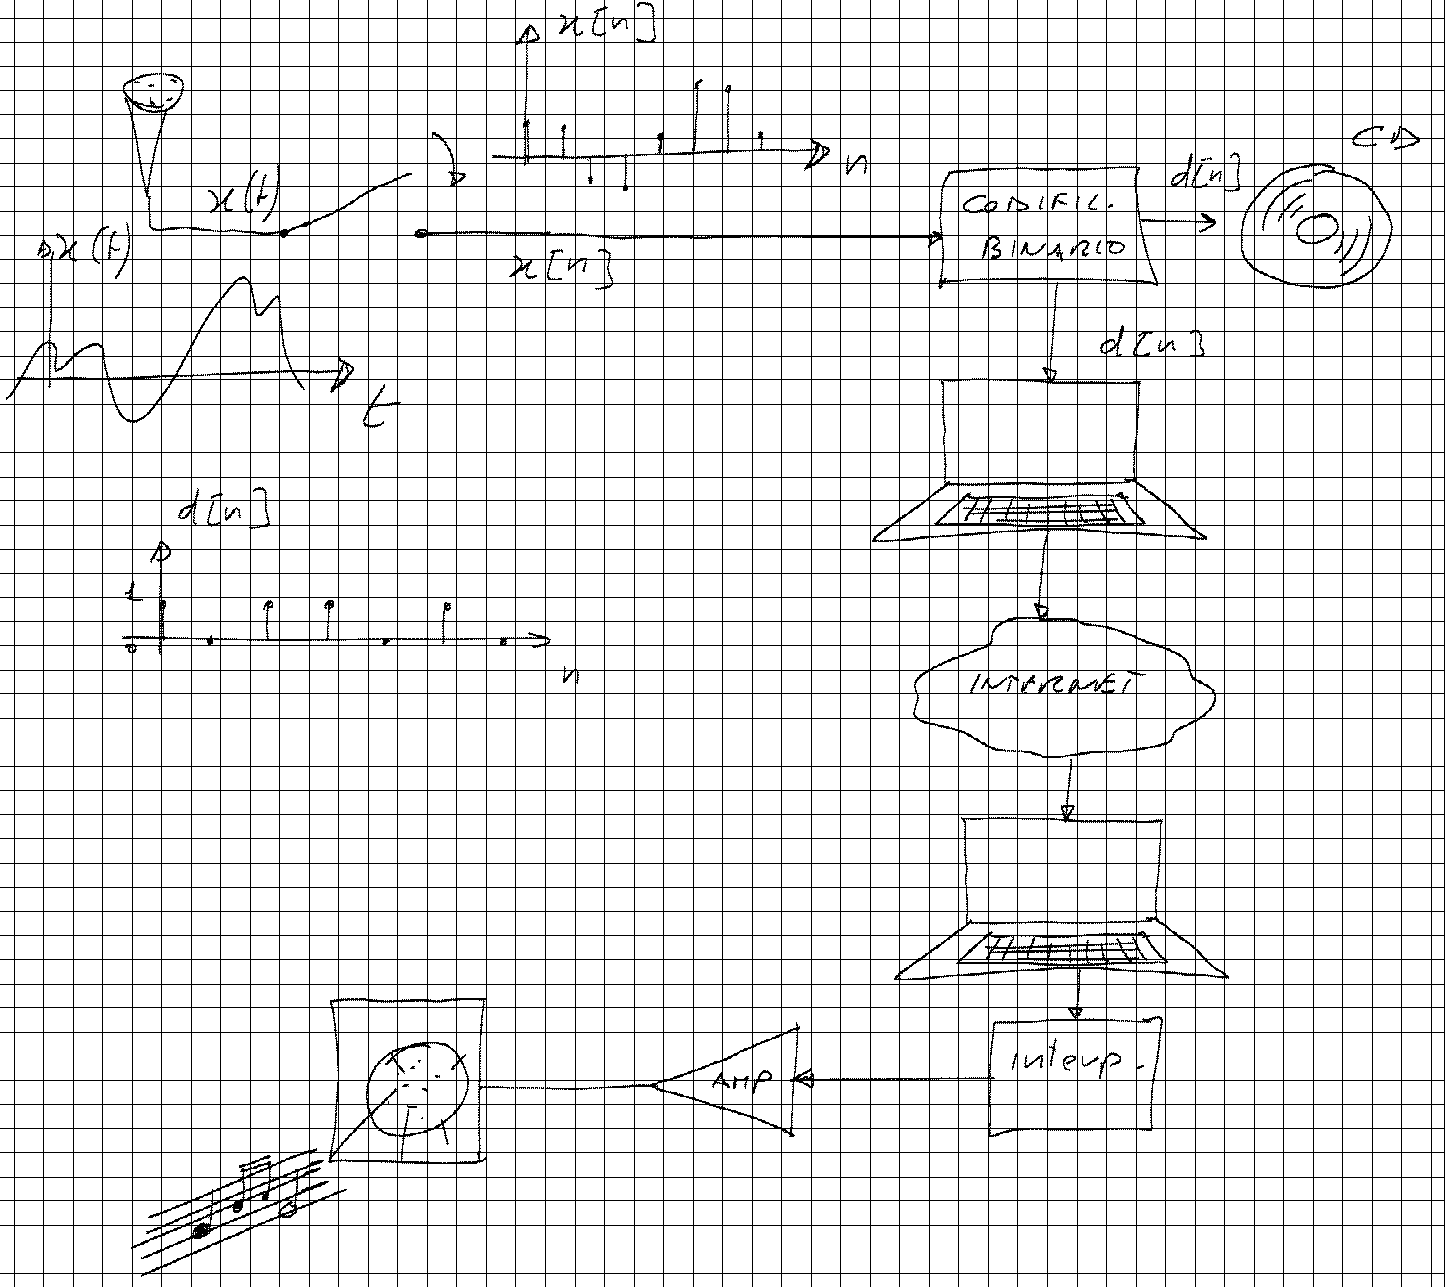
\includegraphics[width=0.9\textwidth]{segnali-05}
\caption{Un sistema di elaborazione e trasmissione dell'informazione.}
\label{fig:sistema-di-elaborazione-e-trasmissione}
\end{figure}


\section{Propriet� dei segnali deterministici}

Analizziamo ora alcune propriet� dei segnali deterministici analogici.
Dato un segnale $x(t)$ (reale o complesso) ne definiamo innanzitutto la \emph{potenza istantanea}:
%
\begin{equation}
P_x(t)\triangleq\abs{x(t)}^{2}   \label{eq:potenza-istant-segnale}
\end{equation}
%
In ottica di rimanere astratti e indipendenti dalla realt� del fenomeno fisico rappresentato, la potenza definita in eq.~\eqref{eq:potenza-istant-segnale} � indipendente dalla grandezza fisica cui si riferisce il segnale. Ci� significa che la potenza che definiamo non � effettivamente misurabile in watt, anzi non lo � quasi mai: sar� poi legata all'effettiva potenza tramite delle costanti.

L'\emph{energia} di un segnale � definita come:
%
\begin{equation}\label{eq:energia-segnale}
E_x \triangleq\int_{-\infty}^{+\infty}P_x(t)\ud t =\int_{-\infty}^{+\infty}\abs{x(t)}^{2}\ud t
\end{equation}
%
Segnali fisici, ossia segnali che rappresentano le grandezze effettivamente osservabili in natura, hanno tutti energia finita ($E_x < \infty$). Segnali ideali possono avere invece anche energia infinita ($E_x = \infty$). Questi ultimi sono delle astrazioni o idealizzazioni di alcuni sistemi, come ad esempio il generatore di tensione ideale, che genera una tensione costante $V$ su tutto l'asse dei tempi:
%
\[x(t)=V \text{ per } -\infty<t<+\infty \qquad\Rightarrow\qquad E_x=\infty\]
%
Ma in realt� nessun generatore viene costruito a $-\infty$ n� dura fino a $+\infty$.

Per caratterizzare dal punto di visto energetico i segnali a energia infinita, si introduce il concetto di
``segnale troncato nel tempo''. Consideriamo due generatori ideali $V_1$ e $V_2$ che hanno entrambi energia
(secondo la definizione appena data) infinita: a causa di ci� essi risulterebbero energeticamente equivalenti
(pur essendo segnali diversi). Per evitare ci� e consentire confronti tra i due, si fa in realt� riferimento a
versioni troncate dei segnali:
%
\[x_p(t)=\begin{cases} x(t) & -\frac{T}{2}\leq t\leq\frac{T}{2}\\0 & \textrm{altrove.}\end{cases}\]
%
L'\emph{energia di un segnale troncato} nel tempo � quindi:
%
\begin{equation}
E_{x_T} = \int_{-\infty}^{+\infty}\abs{x_p(t)}^{2}\ud t = \int_{-\frac{T}{2}}^{+\frac{T}{2}}\abs{x(t)}^{2}\ud t
\end{equation}
%
che � finita (si suppone che il segnale assuma solo valori finiti), mentre:
%
\[E_x = \lim_{T\to\infty} E_{x_T} = \infty.\]
%
La \emph{potenza del segnale troncato} vale:
%
\begin{equation}
P_{x_T}\triangleq\frac{E_{x_T}}{T}
\end{equation}
%
e la \emph{potenza media} � definita come:
%
\begin{equation}\label{eq:potenza-media-segnale}
P_x\triangleq\lim_{T\to\infty}P_{x_T}=
      \lim_{T\to\infty}\frac{E_{x_T}}{T}=
      \lim_{T\to\infty}\frac{1}{T}\int_{-\frac{T}{2}}^{\frac{T}{2}}\abs{x(t)}^2 \ud t.
\end{equation}

Si osservi che tra energia e potenza valgono le seguenti implicazioni:
%
\begin{align*}
P_x=k \qquad \Rightarrow \qquad E_x=\infty\\
E_x<\infty \qquad \Rightarrow \qquad P_x=0
\end{align*}
%
ossia un segnale a potenza finita avr� necessariamente energia infinita, mentre un segnale a energia finita avr� sempre potenza nulla. La motivazione di ci� � semplice da capire:
%
\begin{align*}
P_x=\lim_{T\to\infty}P_{x_T}=\lim_{T\to\infty}\frac{E_{x_T}}{T}=k \qquad \Rightarrow \qquad \lim_{T\to\infty}E_{x_T}=\infty\\
E_x=\lim_{T\to\infty}E_{x_T}=\lim_{T\to\infty}P_{x_T}T=k \qquad \Rightarrow \qquad \lim_{T\to\infty}P_{x_T}=0.
\end{align*}

Per i segnali a potenza finita si definisce anche il \emph{valore efficace} (� quel valore che dovrebbe assumere un segnale costante per avere lo stesso contenuto in potenza del segnale dato):
%
\begin{equation}
x_\mathrm{eff}\triangleq\sqrt{P_x}
\end{equation}

L'ultimo parametro che definiamo � il \emph{valor medio} temporale:
%
\begin{equation}
x_\mathrm{m}\triangleq\lim_{T\to\infty}\frac{1}{T}\int_{-\frac{T}{2}}^{+\frac{T}{2}} x(t)\ud t.
\end{equation}


\section{Segnali tipici}

\subsection{Costante}
$x(t)=A$, con $A\in\R$
\begin{align*}
P_x(t) & =A^2\\
E_x & =\int_{-\infty}^{+\infty}A^2\ud t=\infty\\
P_x & = \lim_{T\to\infty}\frac{E_{x_T}}{T}=\lim_{T\to\infty}\frac{1}{T}\int_{-\frac{T}{2}}^{+\frac{T}{2}}A^2\ud t
                    = \lim_{T\to\infty}\frac{1}{T}A^2T=A^2\\
x_\mathrm{eff} &=\sqrt{A^2}=A\\
x_\mathrm{m} &=\lim_{T\to\infty}\frac{1}{T}\int_{-\frac{T}{2}}^{+\frac{T}{2}}A\ud t=\lim_{T\to\infty}\frac{1}{T}AT=A
\end{align*}


\subsection{Sinusoide}
Prendiamo in esame un segnale sinusoidale
%
\[x(t)=A\cos(2\pi f_0t+\varphi)\]
%
e calcoliamone i parametri energetici. Potenza istantanea e potenza media sono:
%
\begin{align*}
P_x(t)&=A^2\cos^2(2\pi f_0t+\varphi)\\
P_x & = \lim_{T\to\infty}\frac{1}{T}\int_{-\infty}^{+\infty}A^2\cos^2(2\pi f_0t+\varphi)\ud t\\
    & = \lim_{T\to\infty}\frac{A^2}{T}\int_{-\frac{T}{2}}^{+\frac{T}{2}}\frac{1}{2}\ud t+
        \lim_{T\to\infty}\frac{A^2}{T}\int_{-\frac{T}{2}}^{+\frac{T}{2}}\frac{1}{2}\cos(4\pi f_0t+2\varphi)\ud t\\
\intertext{e procedendo in modo non rigorosamente matematico, si pu� ``sdoppiare'' il secondo limite, scrivendo:}
    & = \lim_{T\to\infty}\frac{A^2}{T}\frac{T}{2}+
        \frac{A^2}{2}\frac{\displaystyle\lim_{T\to\infty}\int_{-\frac{T}{2}}^{+\frac{T}{2}}\cos(4\pi f_0t+2\varphi)\ud t}
                          {\displaystyle\lim_{T\to\infty}T}=
        \frac{A^2}{2}
\end{align*}
%
Infatti il denominatore del secondo termine tende all'infinito, mentre il numeratore � una forma s� indefinita, ma comunque limitata:
%
\begin{align*}
 & \lim_{T\to\infty}\int_{-\frac{T}{2}}^{+\frac{T}{2}}\cos(4\pi f_0t+2\varphi)\ud t=
     \lim_{T\to\infty}\left.\frac{1}{4\pi f_0}\sin(4\pi f_0t+2\varphi)\right|_{-\frac{T}{2}}^{+\frac{T}{2}}
\end{align*}
%
dovunque si calcoli il seno esso � sempre compreso tra $-1$ e $1$.

L'energia
%
\begin{align*}
E_x & = \int_{-\infty}^{+\infty}A^2\cos^2(2\pi f_0t+\varphi)\ud t\\
    & = -A^2\underbrace{\int_{-\infty}^{+\infty}\frac{1}{2}\ud t}_{\infty}+
         A^2\underbrace{\int_{-\infty}^{+\infty}\frac{1}{2}\cos(4\pi f_0t+2\varphi)\ud t}_{0}=\infty\\
\end{align*}
%
� infinita, come si poteva affermare gi� non appena era stata calcolata la potenza, che si era trovata finita non nulla.

Il valor efficace e il valor medio sono rispettivamente:
%
\begin{align*}
x_\mathrm{eff}&=\sqrt{\frac{A^2}{2}}=\frac{A}{\sqrt{2}}\\
x_\mathrm{m} & = \lim_{T\to\infty}\frac{1}{T}\int_{-\frac{T}{2}}^{+\frac{T}{2}}A\cos(2\pi f_0t+\varphi)\ud t\\
    & = \frac{\lim_{T\to\infty}\int_{-\frac{T}{2}}^{+\frac{T}{2}}\cos(2\pi f_0t+\varphi)\ud t}{\lim_{T\to\infty}T}=0\\
\end{align*}
%
dove per il calcolo del valor medio abbiamo nuovamente sdoppiato un limite.


\subsection{Gradino}
\label{sub:gradino}
La funzione gradino, indicata con $\u(t)$, � definita come:
%
\[\u(t)=\begin{cases}1&t\geq 0\\0&t<0.\end{cases}\]
%
Bench� esistano in realt� altre definizioni di gradino, relativamente al valore che assume in $0$ (ad esempio
una per cui in $0$ vale la met� del valore massimo), nulla cambia ai fini delle valutazioni energetiche.

\begin{figure}[b]
\centering
\framebox{\begin{pspicture*}(-2.8,-0.6)(5.8,1.9)
  \psaxes[linewidth=0.4pt,labels=none,ticks=none]{->}(0,0)(-2.5,-0.4)(5.5,1.7)
  \psline[linewidth=1pt](0,0.8)(4,0.8)
  \psline[linewidth=1pt](0,0)(-1,0)
  \psline[linewidth=1pt,linestyle=dashed,dash=2pt 2pt](-1,0)(-2.2,0)
  \psline[linewidth=1pt,linestyle=dashed,dash=2pt 2pt](4,0.8)(5.2,0.8)
  \uput[l](0,1.5){$\u(t)$}
  \uput[d](5.4,0){$t$}
  \uput[l](0,0.8){$1$}
\end{pspicture*}}
\caption{Rappresentazione grafica della funzione gradino.}
\end{figure}

La potenza istantanea e la potenza media sono:
%
\begin{align*}
P_x(t) & = \u^2(t)=\u(t)\\
P_x    & = \lim_{T\to\infty}\frac{1}{T}\int_{-\frac{T}{2}}^{+\frac{T}{2}}\u^2(t)\ud t=
           \lim_{T\to\infty}\frac{1}{T}\int_{0}^{\frac{T}{2}}\ud t=
           \lim_{T\to\infty}\frac{1}{T}\frac{T}{2}=\frac{1}{2}
\end{align*}

L'energia sar� quindi infinita:
%
\[E_x=\int_{-\infty}^{+\infty}\u^2(t)\ud t=\int_{-\infty}^{+\infty}\u(t)\ud t=\int_{0}^{+\infty}\ud t=\infty\]

Valore efficace e valor medio sono:
%
\begin{align*}
x_\mathrm{eff} & =\frac{1}{\sqrt{2}}\\
x_\mathrm{m} & = \lim_{T\to\infty}\frac{1}{T}\int_{-\frac{T}{2}}^{+\frac{T}{2}}\u(t)\ud t=
        \lim_{T\to\infty}\frac{1}{T}\int_{0}^{+\frac{T}{2}}\ud t=
        \lim_{T\to\infty}\left.\frac{1}{T}\cdot t\,\right|_{0}^{\frac{T}{2}}=
        \frac{1}{2}
\end{align*}


\subsection{Rettangolo}
La funzione rettangolo $\rect{t}{T_0}$ � definita nel seguente modo:
%
\[\rect{t}{T_0}=\begin{cases}1 & -\frac{T_0}{2}\leq t\leq\frac{T_0}{2}\\0 & \textrm{altrove}\end{cases}\]
%
dove la $t$ � la variabile indipendente, mentre $T_0$ � un parametro che indica la durata temporale della \textit{rect}.

\begin{figure}
\centering
\framebox{\begin{pspicture*}(-4.3,-0.6)(4.3,1.9)
  \psaxes[linewidth=0.4pt,labels=none,ticks=none]{->}(0,0)(-4.1,-0.4)(4,1.7)
  \psline[linewidth=1pt](-1,0.8)(1,0.8)
  \psline[linewidth=0.5pt](1,0.8)(1,0)
  \psline[linewidth=0.5pt](-1,0.8)(-1,0)
  \psline[linewidth=1pt](-1,0)(-2.5,0)
  \psline[linewidth=1pt](1,0)(2.5,0)
  \psline[linewidth=1pt,linestyle=dashed,dash=2pt 2pt](-2.5,0)(-3.5,0)
  \psline[linewidth=1pt,linestyle=dashed,dash=2pt 2pt](2.5,0)(3.5,0)
  \uput[l](0,1.5){$x(t)$}
  \uput[d](3.9,0){$t$}
  \uput[u](0.4,0.8){$1$}
  \uput[d](-1,0){$\scriptstyle{-T_0/2}$}
  \uput[d](1,0){$\scriptstyle{+T_0/2}$}
\end{pspicture*}}
\caption{Rappresentazione grafica della funzione rettangolo.}
\end{figure}

Notiamo innanzitutto che il quadrato della funzione rettangolo � uguale alla funzione stessa:
%
\[\vrect^2\biggl(\frac{t}{T_0}\biggr)=\rect{t}{T_0}\]
%
e pertanto otteniamo che la potenza istantanea vale:
%
\[P_x(t) = \abs{x(t)}^2 = \rect{t}{T_0}\]
%
mentre la potenza media risulta uguale al valore medio ed �:
%
\[P_x = x_\mathrm{m} = \lim_{T\to\infty}\frac{1}{T}\int_{-\frac{T}{2}}^{+\frac{T}{2}}\rect{t}{T_0}\ud t=0\]
%
Quest'ultimo risultato lo si comprende considerando il seguente grafico:
%
\begin{center}\framebox{\setlength{\unitlength}{1mm}
\begin{pspicture*}(-5.3,-0.6)(5.5,1.9)
  \pscustom[linewidth=0.5pt,fillstyle=solid,fillcolor=lightgray]{%
    \psline[linewidth=0.5pt](-1,0)(-1,0.8)
    \psline[linewidth=1pt](-1,0.8)(1,0.8)
    \psline[linewidth=0.5pt](1,0.8)(1,0)}
  \psaxes[linewidth=0.4pt,labels=none,ticks=none]{->}(0,0)(-5.1,-0.4)(5.2,1.7)
  \psline[linewidth=1pt](-2.5,0.8)(2.5,0.8)
  \psline[linewidth=0.5pt](2.5,0.8)(2.5,0)
  \psline[linewidth=0.5pt](-2.5,0.8)(-2.5,0)
  \psline[linewidth=1pt](-2.5,0)(-3.8,0)
  \psline[linewidth=1pt](2.5,0)(3.8,0)
  \psline[linewidth=1pt,linestyle=dashed,dash=2pt 2pt](-3.8,0)(-4.8,0)
  \psline[linewidth=1pt,linestyle=dashed,dash=2pt 2pt](3.8,0)(4.8,0)
  \uput[l](0,1.5){$x(t)$}
  \uput[d](5.1,0){$t$}
  \uput[u](0.4,0.8){$1$}
  \uput[d](-1,0){$\scriptstyle{-T/2}$}
  \uput[d](1,0){$\scriptstyle{+T/2}$}
  \uput[d](-2.5,0){$\scriptstyle{-T_0/2}$}
  \uput[d](2.5,0){$\scriptstyle{+T_0/2}$}
\end{pspicture*}}\end{center}
%
Infatti:
%
\begin{equation*}
\int_{-\frac{T}{2}}^{+\frac{T}{2}}\rect{t}{T_0}\ud t=
    \begin{cases}T&\text{se }T<T_0\\T_0&\text{se }T\geq T_0\end{cases}
\end{equation*}
%
e perci�, nella formula precedente, il limite del rapporto tra l'integrale (che tende a $T_0$) e $T$ (che tende a infinito) vale zero.

L'energia vale invece:
%
\[E_x = \int_{-\infty}^{+\infty}\rect{t}{T_0}\ud t=T_0\]
%
Se prima della potenza si fosse calcolata l'energia, trovandola finita avremmo potuto concludere subito che la potenza � nulla. Infine:
%
\[x_\mathrm{eff}=0\]


\subsection{Esponenziale unilatera}
La funzione esponenziale unilatera � definita come:
%
\[x(t)=\e^{-t}\u(t).\]
%
Il suo grafico � riportato in figura~\ref{fig:esponenziale-unilatera}.
%
\begin{figure}
\centering
\framebox{\begin{pspicture*}(-2.8,-0.6)(5.8,1.9)
  \psaxes[linewidth=0.4pt,labels=none,ticks=none]{->}(0,0)(-2.5,-0.4)(5.5,1.7)
  \psline[linewidth=1pt](-2.2,0)(0,0)
  \psplot[linewidth=1pt,plotstyle=curve,plotpoints=200]% 0.5*e^(-x)
         {0}{5.2}{1 2.718281828459045235 x neg exp mul}
  \uput[l](0,1.5){$x(t)$}
  \uput[d](5.4,0){$t$}
\end{pspicture*}}
\caption{Grafico della funzione esponenziale unilatera.}
\label{fig:esponenziale-unilatera}
\end{figure}
%
Potenza istantanea ed energia valgono:
%
\begin{align*}
P_x(t) & =\e^{-2t}\u(t)\\
E_x & =\int_{-\infty}^{+\infty}\e^{-2t}\u(t)\ud t=\int_{0}^{+\infty}\e^{-2t}\ud t=\left.-\frac{1}{2}\e^{-2t}\right|_{0}^{\infty}=\frac{1}{2}
\end{align*}
%
Di conseguenza la potenza media del segnale � nulla:
%
\begin{align*}
P_x & = \lim_{T\to\infty}\frac{1}{T}\int_{-\frac{T}{2}}^{+\frac{T}{2}}\e^{-2t}\u(t)\ud t=
        \lim_{T\to\infty}\frac{1}{T}\int_{0}^{\frac{T}{2}}\e^{-2t}\ud t\\
    & = \lim_{T\to\infty}\frac{1}{T}\left(-\frac{1}{2}\right)\left.\e^{-2t}\right|_{0}^{\frac{T}{2}}=
        \lim_{T\to\infty}-\frac{1}{2T}\left(\e^{-T}-1\right)=0
\end{align*}
%
e lo stesso il suo valore efficace:
%
\[x_\mathrm{eff} = 0\]
%
Anche il valor medio � nullo:
%
\begin{align*}
x_\mathrm{m} & = \lim_{T\to\infty}\frac{1}{T}\int_{-\frac{T}{2}}^{+\frac{T}{2}}\e^{-t}\u(t)\ud t=
        \lim_{T\to\infty}\frac{1}{T}\int_{0}^{\frac{T}{2}}\e^{-t}\ud t\\
    & = \lim_{T\to\infty}\frac{1}{T}(-1)\left.\e^{-t}\right|_{0}^{\frac{T}{2}}=
        -\frac{1}{T}\left(\e^{-\frac{T}{2}}-1\right)=0
\end{align*}

\subsection{Esponenziale bilatera}
L'esponenziale bilatera �:
%
\[x(t)=\e^{-\abs{t}}.\]
%
\begin{figure}
\centering
\framebox{\begin{pspicture*}(-4.8,-0.6)(4.8,1.9)
  \psaxes[linewidth=0.4pt,labels=none,ticks=none]{->}(0,0)(-4.5,-0.4)(4.5,1.7)
  \psplot[linewidth=1pt,plotstyle=curve,plotpoints=200]% 0.5*\e^(-abs(x))
         {-4.2}{0}{1 2.718281828459045235 x abs neg exp mul}
  \psplot[linewidth=1pt,plotstyle=curve,plotpoints=200]% 0.5*\e^(-abs(x))
         {0}{4.2}{1 2.718281828459045235 x abs neg exp mul}
  \uput[l](0,1.5){$x(t)$}
  \uput[d](4.4,0){$t$}
\end{pspicture*}}
\caption{Rappresentazione grafica della funzione esponenziale bilatera.}
\label{fig:esponenziale-bilatera}
\end{figure}
%
\begin{align*}
P_x(t) &=\e^{-2\abs{t}}\\
E_x & =\int_{-\infty}^{+\infty}\e^{-2\abs{t}}\ud t=2\int_{0}^{+\infty}\e^{-2t}\ud t=1\\
P_x & =\lim_{T\to\infty}\frac{1}{T}\int_{-\frac{T}{2}}^{+\frac{T}{2}}\e^{-2\abs{t}}\ud t=
     \lim_{T\to\infty}\frac{2}{T}\int_{0}^{+\frac{T}{2}}\e^{-2t}\ud t=0\\
x_\mathrm{eff} & =0\\
x_\mathrm{m} &= \lim_{T\to\infty}\frac{1}{T}\int_{-\frac{T}{2}}^{+\frac{T}{2}}\e^{-\abs{t}}\ud t=
       \lim_{T\to\infty}\frac{2}{T}\int_{0}^{+\frac{T}{2}}\e^{-t}\ud t=0
\end{align*}

\subsection{Segno*}
La funzione \textit{segno} � definita come:
%
\[\sgn(t)=\begin{cases}1&t\geq 0\\-1&t<0\end{cases}\]
%
\begin{figure}
\centering
\framebox{\begin{pspicture*}(-4.3,-1)(4.3,1.5)
  \psaxes[linewidth=0.4pt,labels=none,ticks=none]{->}(0,0)(-4.1,-0.8)(4,1.3)
  \psline[linewidth=1pt](0,0.5)(2.5,0.5)
  \psline[linewidth=1pt](0,-0.5)(-2.5,-0.5)
  \psline[linewidth=1pt,linestyle=dashed,dash=2pt 2pt](-2.5,-0.5)(-3.7,-0.5)
  \psline[linewidth=1pt,linestyle=dashed,dash=2pt 2pt](2.5,0.5)(3.7,0.5)
  \uput[l](0,1.1){$\sgn(t)$}
  \uput[d](3.9,0){$t$}
  \uput[l](0,0.5){$1$}
  \uput[r](0,-0.5){$-1$}
\end{pspicture*}}
\caption{Rappresentazione della funzione segno.}
\end{figure}
%
\begin{align*}
P_x(t) &=1\\
E_x &=\int_{-\infty}^{+\infty}1\ud t=\infty\\
P_x &=1\\
x_\mathrm{eff}&=1\\
x_\mathrm{m} & = \lim_{T\to\infty}\frac{1}{T}\int_{-\frac{T}{2}}^{+\frac{T}{2}}\sgn(t)\ud t=
        \lim_{T\to\infty}\frac{1}{T}\left(\frac{T}{2}-\frac{T}{2}\right)=0
\end{align*}


\section[Relazione tra \texorpdfstring{$P_x$, $x_\mathrm{eff}$ e $x_\mathrm{m}$}%
                                      {potenza media, valore efficace e valor medio}]%
        {Relazione tra potenza media, valore efficace e valor medio}

Osservando i vari casi analizzati, si pu� constatare che laddove la potenza media sia nulla, anche il valor medio e il valore efficace sono risultati nulli. Si pu� dimostrare che questa propriet� � vera in generale.

\begin{proposizione}
Dato un qualsiasi segnale $x(t)$, vale l'implicazione:
\[P_x=0 \quad\Rightarrow\quad \left\{\begin{array}{l}x_\mathrm{eff}=0\\x_\mathrm{m}=0.\end{array}\right.\]
\end{proposizione}
\begin{proof}
La dimostrazione per il valore efficace � banale. Per il valor medio, possiamo scomporre il generico segnale
$x(t)$ come
\[x(t)=x_\mathrm{m}+x'(t)\]
ossia come somma della sua media $x_\mathrm{m}$ pi� un segnale $x'(t)\triangleq x(t)-x_\mathrm{m}$ (il quale rappresenta
le variazioni del segnale originario rispetto alla sua media). Il segnale $x'(t)$ ha media nulla:
\begin{align*}
 & \lim_{T\to\infty}\frac{1}{T}\int_{-\frac{T}{2}}^{+\frac{T}{2}}x'(t)\ud t=
        \lim_{T\to\infty}\frac{1}{T}\int_{-\frac{T}{2}}^{+\frac{T}{2}}[x(t)-x_\mathrm{m}]\ud t\\
 &\quad =\underbrace{\lim_{T\to\infty}\frac{1}{T}\int_{-\frac{T}{2}}^{+\frac{T}{2}}x(t)\ud t}_{x_\mathrm{m}}-
        \lim_{T\to\infty}\frac{1}{T}\int_{-\frac{T}{2}}^{+\frac{T}{2}}x_\mathrm{m}\ud t\\
 &\quad =x_\mathrm{m} - \lim_{T\to\infty}\frac{1}{T}x_\mathrm{m} T=x_\mathrm{m}-x_\mathrm{m}=0.
\end{align*}
La dimostrazione si effettua partendo dall'espressione della potenza media, riscrivendola in
un determinato modo e imponendo infine che sia nulla.
\begin{align*}
P_x = & \lim_{T\to\infty}\frac{1}{T}\int_{-\frac{T}{2}}^{+\frac{T}{2}}\abs{x(t)}^2\ud t=
        \lim_{T\to\infty}\frac{1}{T}\int_{-\frac{T}{2}}^{+\frac{T}{2}}\abs{x_\mathrm{m}+x'(t)}^2\ud t\\
 \intertext{ma poich� $\abs{z}^2=z\cdot z^*$ e $(z_1+z_2)^*=z_1^*+z_2^*$, otteniamo:}
    = & \lim_{T\to\infty}\frac{1}{T}\int_{-\frac{T}{2}}^{+\frac{T}{2}}\left(x_\mathrm{m}+x'(t)\right)\left(x_\mathrm{m}^*+x'^*(t)\right)\ud t\\
    = & \lim_{T\to\infty}\frac{1}{T}\int_{-\frac{T}{2}}^{+\frac{T}{2}}\left[\abs{x_\mathrm{m}}^2+\abs{x'(t)}^2 +
        x_\mathrm{m}x'^*(t)+ x_\mathrm{m}^*x'(t)\right]\ud t
\end{align*}
nella quale compare un'espressione del tipo $z_1z_2^*+z_1^*z_2$. Siccome $(z_1z_2)^*=z_1^*z_2^*$, allora:
\begin{align*}
z_1z_2^*+z_1^*z_2 & = z_1z_2^*+(z_1z_2^*)^*=z+z^*    \tag{$z\triangleq z_1z_2^*$}\\
                  & = 2\Re\{z\} = 2\Re\{z_1z_2^*\}.
\end{align*}
Infatti, se $z=a+\j b$, allora $a=\Re\{z\}=\frac{1}{2}(z+z^*)$. Tornando quindi alla potenza scriviamo:
\begin{align*}
P_x = & \lim_{T\to\infty}\frac{1}{T}\int_{-\frac{T}{2}}^{+\frac{T}{2}}\left[\abs{x_\mathrm{m}}^2+\abs{x'(t)}^2 +
        2\Re\left\{x_\mathrm{m}^*x'(t)\right\}\right]\ud t\\
    = & \lim_{T\to\infty}\frac{1}{T}\int_{-\frac{T}{2}}^{+\frac{T}{2}}\abs{x_\mathrm{m}}^2\ud t+
        \lim_{T\to\infty}\frac{1}{T}\int_{-\frac{T}{2}}^{+\frac{T}{2}}\abs{x'(t)}^2\ud t\\
      & +2\Re\Bigg\{x_\mathrm{m}^*\underbrace{\lim_{T\to\infty}\frac{1}{T}\int_{-\frac{T}{2}}^{+\frac{T}{2}}x'(t)\ud t}_{0}\Bigg\}\\
    = & \abs{x_\mathrm{m}}^2+P_{x'}
\end{align*}
Deve quindi essere:
\begin{align*}
 P_x= & \abs{x_\mathrm{m}}^2+P_{x'} = 0
\end{align*}
dove sia $\abs{x_\mathrm{m}}^2$ che $P_{x'}$ sono numeri non negativi ($\geq 0$) essendo integrali di funzioni
($|\cdot|^2$) sempre maggiori o uguali a zero. Affinch� loro somma sia nulla, devono esser per forza nulli
entrambi e pertanto, in particolare, � nullo il valor medio $x_\mathrm{m}$.
\end{proof}

Quanto appena dimostrato pu� essere espresso in altri termini dicendo che condizioni necessarie affinch� $P_x=0$ sono che il segnale $x(t)$ sia a media e a valore efficace nulli.


% !TeX encoding = ISO-8859-1
% !TeX root = appunti.tex

\chapter{Analisi di segnali periodici}
\label{cha:segnali-periodici}


\section{Concetti generali}

Un segnale $x(t)$ si dice periodico se esiste un $T_0$ tale che sia soddisfatta la relazione:
%
\begin{equation}
x(t)=x(t-kT_0)
\end{equation}
%
per ogni $k$ intero. Il valore $T_0$ � detto \emph{periodo} del segnale ed � l'inverso della frequenza $f_0\triangleq 1/T_0$.

� facile verificare che l'energia $E_x$ di un segnale periodico (cos� come definita nel capitolo precedente) � in generale infinita:
%
\begin{align*}
E_x & = \int_{-\infty}^{+\infty}|x(t)|^2\ud t=
        \sum_{k=-\infty}^{+\infty}\int_{-\frac{T_0}{2}+kT_0}^{+\frac{T_0}{2}+kT_0}|x(t)|^2\ud t=
        \sum_{k=-\infty}^{+\infty}E_{x_k}=\infty.
\end{align*}

In generale, invece, la potenza media � finita, e potrebbe essere calcolata usando l'eq.~\eqref{eq:potenza-media-segnale}. Si dimostra che eseguendo il limite si giunge a un risultato pi� semplice:
%
\begin{align}
P_x & = \lim_{T\to\infty}\frac{E_{x_T}}{T}=
        \lim_{T\to\infty}\frac{1}{T}\int_{-\frac{T}{2}}^{+\frac{T}{2}}|x(t)|^2\ud t \notag
\intertext{e discretizzando la variabile $T=kT_0$, si ottiene:}
    & = \lim_{k\to\infty}\frac{1}{kT_0}\int_{-\frac{kT_0}{2}}^{+\frac{kT_0}{2}}|x(t)|^2\ud t  \notag
\intertext{che equivale calcolare l'integrale su $k$ periodi:}
    & = \lim_{k\to\infty}\frac{1}{kT_0}k\int_{-\frac{T_0}{2}}^{+\frac{T_0}{2}}|x(t)|^2\ud t \notag\\
    & = \frac{1}{T_0}\int_{-\frac{T_0}{2}}^{+\frac{T_0}{2}}|x(t)|^2\ud t.
\end{align}

Anche l'espressione del valor medio di un segnale periodico si semplifica:
%
\begin{align}\label{eq:valor-medio-periodico}
x_m\triangleq\lim_{T\to\infty}\frac{1}{T}\int_{-\frac{T}{2}}^{+\frac{T}{2}}x(t)\ud t=\frac{1}{T_0}
     \int_{-\frac{T_0}{2}}^{+\frac{T_0}{2}}x(t)\ud t.
\end{align}


\section{Analisi di Fourier}

L'analisi fasoriale consente di analizzare circuiti lineari (ossia circuiti per i quali � valida la sovrapposizione degli effetti) quando il segnale applicato � una somma finita di componenti sinusoidali.
L'analisi di Fourier consente di studiare circuiti ai quali sia applicato un generico segnale periodico (con andamento arbitrario, anche non sinusoidale).

Ciascun segnale periodico di periodo $T_0$ che soddisfi il ``criterio di Dirichlet'' (il criterio~\ref{thm:criterio-dirichelet-sulla-TSF} definito pi� avanti) pu� essere scritto come la somma di infinite sinusoidi a frequenze multiple di $1/T_0$.
%
\begin{align}
x(t) & = \sum_{n=0}^{\infty}A_n\cos(2\pi nf_0t+\varphi_n)\\
     & = A_0 + \sum_{n=1}^{\infty}A_n\cos(2\pi nf_0t+\varphi_n)  \label{eq:ssf-forma-polare}
\end{align}
%
dove $f_0=1/T_0$ � la \emph{frequenza fondamentale}.
La relazione~\eqref{eq:ssf-forma-polare} costituisce l'\emph{espressione in forma polare dello sviluppo in serie di Fourier}, nella quale un segnale periodico reale $x(t)$ � rappresentato come somma di un termine costante $A_0$ (\emph{componente continua}) e di una serie di termini sinusoidali, le \emph{oscillazioni armoniche} (o semplicemente \emph{armoniche}). L'$n$-esima armonica ha ampiezza $A_n>0$, frequenza $nf_0$ e fase $\varphi_n$. La componente in continua coincide con il valor medio del segnale:
%
\begin{align*}
x_m &= \frac{1}{T_0}\int_{-\frac{T_0}{2}}^{+\frac{T_0}{2}}x(t)\ud t\\
    &= \frac{1}{T_0}\int_{-\frac{T_0}{2}}^{+\frac{T_0}{2}}A_0\ud t +
       \underbrace{\frac{1}{T_0}\int_{-\frac{T_0}{2}}^{+\frac{T_0}{2}}A_1\cos(2\pi f_0t+\varphi_1)\ud t}_{0}\\
    &\phantom{=\;} +\underbrace{\frac{1}{T_0}\int_{-\frac{T_0}{2}}^{+\frac{T_0}{2}}
                   A_2\cos(4\pi f_0t+\varphi_2)\ud t}_{0}+\dots=
       \frac{1}{T_0}\int_{-\frac{T_0}{2}}^{+\frac{T_0}{2}}A_0\ud t = A_0
\end{align*}


\subsection{Il Criterio di Dirichelet}

Dato un segnale periodico, affinch� la serie di eq.~\eqref{eq:ssf-forma-polare} converga uniformemente e il segnale stesso sia rappresentabile secondo la forma polare di Fourier, devono essere soddisfatte determinate condizioni, racchiuse nel ``Criterio di Dirichelet''. Si tratta di un criterio sufficiente costituito da un insieme di tre condizioni.

\begin{criterio}[di Dirichelet]
\label{thm:criterio-dirichelet-sulla-TSF}
Se
\begin{enumerate}
\item $x(t)$ � assolutamente integrabile sul periodo $T_0$, ossia
      \[\int_{-T_0/2}^{+T_0/2}\abs{x(t)}\ud t<\infty,\]
\item $x(t)$ � continua o presenta un numero finito di discontinuit� di prima
      specie\footnote{Limite destro e sinistro devono cio� essere (diversi ma) finiti.} nel periodo $T_0$,
\item $x(t)$ � derivabile su tutto il periodo escluso al pi� un numero finito di punti nei quali esistono
      finite le derivate destra e sinistra
\end{enumerate}
oppure
\begin{enumerate}
\item[3.] $x(t)$ ha un numero finito di massimi e minimi nel periodo,
\end{enumerate}
allora la serie di Fourier converge al valore assunto dalla funzione $x(t)$ nei punti in cui questa � continua e alla semisomma dei limiti destro e sinistro nei punti in cui $x(t)$ presenta le eventuali discontinuit� di prima specie.
\end{criterio}

Si noti che i segnali fisici verificano sempre questo criterio. Inoltre, anche segnali a dente di sega (o simili, con discontinuit�) possono esser sviluppati in serie di Fourier.


\subsection{Sviluppo in serie di Fourier in forma complessa}
Usando%
\margincomment{Non � necessario conoscere questi calcoli per l'esame orale.}
le formule di Eulero%
\footnote{Le formule di Eulero consentono di esprimere seno e coseno nella forma:
\[\cos(x) = \frac{\e^{\,\j x}+\e^{-\j x}}{2},\quad\sin(x) = \frac{\e^{\,\j x}-\e^{-\j x}}{2\j}.\]}
%
si pu� riscrivere l'equazione~\eqref{eq:ssf-forma-polare} nella forma:
%
\begin{align*}
x(t) &= A_0+\sum_{n=1}^{\infty}A_n \frac{\e^{\,\j(2\pi nf_0t+\varphi_n)}+\e^{-\j(2\pi nf_0t+\varphi_n)}}{2}\\
     &= A_0+\sum_{n=1}^{\infty}\frac{A_n}{2}\e^{\,\j\varphi_n}\e^{\,\j 2\pi nf_0t}+
            \sum_{n=1}^{\infty}\frac{A_n}{2}\e^{-\j\varphi_n}\e^{-\j 2\pi nf_0t}\\
     &= A_0+\sum_{n=1}^{\infty}\frac{A_n}{2}\e^{\,\j\varphi_n}\e^{\,\j 2\pi nf_0t}+
            \sum_{n=-1}^{-\infty}\frac{A_{-n}}{2}\e^{-\j\varphi_{-n}}\e^{\,\j 2\pi nf_0t}
\end{align*}
%
e definendo:
%
\begin{align*}
\begin{cases}X_0\triangleq A_0, &\\
 X_n\triangleq A_n\e^{\,\j\varphi_n}/2 & \text{per }n=1,2,\dots,\\
 X_n\triangleq A_{-n}\e^{-\j\varphi_{-n}}/2 & \text{per }n=-1,-2,\dots,
\end{cases}
\end{align*}
%
si ottiene:
%
\begin{align}
x(t) &= X_0 + \sum_{n=1}^{+\infty}X_n\e^{\,\j2\pi nf_0t}+\sum_{n=-1}^{-\infty}X_n\e^{\,\j2\pi nf_0t} \notag\\
     &= \sum_{n=-\infty}^{+\infty}X_n\e^{\,\j2\pi nf_0t}  \label{eq:ssf-forma-complessa}
\end{align}
%
che rappresenta l'\emph{espressione in forma complessa della serie di Fourier}. (Notare che abbiamo continuato a considerare $x(t)$ come segnale reale, ma la rappresentazione potrebbe essere estesa anche a segnali complessi.) Questa relazione viene anche detta \ac{ATSF}:

\begin{center}\begin{tabular}{lm{5cm}}
 \framebox[.50\linewidth]{$\displaystyle{x(t)=\sum_{n=-\infty}^{+\infty}X_n\e^{\,\j2\pi nf_0t}}$} &
 \begin{flushleft}\textsc{Antitrasformata Serie di Fourier\\(equazione di sintesi)}\end{flushleft}
\end{tabular}\end{center}

\begin{teorema}
Se $x(t)$ � un segnale periodico esprimibile mediante serie di Fourier, allora i coefficienti $X_n$ della serie possono essere ottenuti mediante la cosiddetta \emph{equazione di analisi}:
%
\begin{center}\begin{tabular}{lm{5cm}}
 \framebox[.50\linewidth]{$\displaystyle{X_n=\frac{1}{T_0}\int_{-\frac{T_0}{2}}^{+\frac{T_0}{2}}x(t)\e^{-\j2\pi nf_0t}\ud t}$} &
 \begin{flushleft}\textsc{Trasformata Serie di Fourier\\(equazione di analisi)}\end{flushleft}
\end{tabular}\end{center}
\end{teorema}
\begin{proof}
Infatti, sostituendo nella trasformata serie di Fourier il segnale $x(t)$ espresso mediante l'equazione di sintesi, si ottengono esattamente i termini $X_n$:
\begin{align*}
\TSF[x(t)] &= \frac{1}{T_0}\int_{-\frac{T_0}{2}}^{+\frac{T_0}{2}}\sum_{m=-\infty}^{+\infty}
              X_m\e^{\,\j2\pi mf_0t}\e^{-\j2\pi nf_0t}\ud t\\
 &= \frac{1}{T_0}\sum_{m=-\infty}^{+\infty}X_m\int_{-\frac{T_0}{2}}^{+\frac{T_0}{2}}
    \e^{\,\j2\pi(m-n)f_0t}\ud t\\
 &= \frac{1}{T_0}\sum_{m=-\infty}^{+\infty}X_m
    \Bigg[\int_{-\frac{T_0}{2}}^{+\frac{T_0}{2}}\cos\bigl(2\pi(m-n)f_0t\bigr)\ud t\\
 &\phantom{=\;}+\j\int_{-\frac{T_0}{2}}^{+\frac{T_0}{2}}\sin\bigl(2\pi(m-n)f_0t\bigr)\ud t\Bigg]\\
 &= \frac{1}{T_0}\cdot X_n\cdot T_0=X_n
\end{align*}
dove le ultime uguaglianze si hanno in quanto:
\begin{align}
 & \int_{-\frac{T_0}{2}}^{+\frac{T_0}{2}}\cos\bigl(2\pi(m-n)f_0t\bigr)\ud t = \begin{cases}T_0 & \text{se }m=n\\0 & \text{se }m\neq n\end{cases}   \label{eq:integrale-coseno}\\
 & \int_{-\frac{T_0}{2}}^{+\frac{T_0}{2}}\sin\bigl(2\pi(m-n)f_0t\bigr)\ud t = \begin{cases}0 & \text{se }m=n\\0 & \text{se }m\neq n.\end{cases}   \label{eq:integrale-seno}
\end{align}
ossia l'integrale sul periodo di seno e coseno � sempre nullo. L'eq.~\eqref{eq:integrale-seno} per $m=n$ si riduce all'integrale (nullo) di una funzione identicamente nulla, mentre l'unico termine non nullo � quello di eq.~\eqref{eq:integrale-coseno} per $m=n$, che si riduce all'integrale di una funzione che vale costantemente $1$.
\end{proof}

La \ac{TSF} � biunivoca, in quanto al segnale analogico $x(t)$ corrisponde univocamente la sequenza complessa $X_n$ e a questa corrisponde esattamente $x(t)$. In breve si indicher� questa corrispondenza con la scrittura:
%
\[x(t)\quad\xLeftrightarrow{\TSF}\quad X_n.\]
%
Ci� comporta che le informazioni contenute nel segnale originario nel dominio del tempo $x(t)$ sono contenute in modo equivalente anche nella sequenza di valori complessi $X_n$.

Si noti inoltre che, come gi� mostrato precedentemente, il termine $X_0=A_0$ nella trasformata serie di Fourier � l'espressione del valor medio per un segnale periodico cos� come calcolato nell'equazione~\eqref{eq:valor-medio-periodico}.


\section{Spettro di un segnale periodico}

Lo \emph{spettro}%
\footnote{Il termine ``spettro'' si intende nel generico senso di ``rappresentazione'', ``visione'', e nasce nel campo della spettroscopia, in cui si analizza la composizione dei materiali attraverso le righe di emissione caratteristiche dei diversi elementi chimici. � usato in questo caso in analogia con le ``righe'' delle rappresentazioni di ampiezza o di fase delle componenti armoniche.}
di un segnale periodico $x(t)$ � una rappresentazione del contenuto frequenziale del segnale stesso. Essendo la $X_n$ una sequenza complessa, per raffigurarla sono necessari in generale due grafici, uno per lo \emph{spettro di ampiezza} ($\abs{X_n}$) e l'altro per lo \emph{spettro di fase} ($\angle X_n$).

Dall'espressione complessa~\eqref{eq:ssf-forma-complessa} dello sviluppo in serie di Fourier risulta chiaramente che una condizione necessaria affinch� la serie di Fourier converga � che l'ampiezza $\abs{X_n}$ delle armoniche tenda a zero per $n\to\infty$, e in virt� di ci� le componenti pi� significative dello spettro sono quelle per $n$ piccolo in modulo. Tipicamente, perci�, lo spettro di ampiezza decresce allontanandosi dall'asse delle ordinate, come rappresentato nella figura~\ref{fig:spettro-di-ampiezza-e-fase-tsf}.

\begin{figure}
\centering
\subfloat{\framebox{\begin{pspicture*}(-3,-0.6)(3,2)
  \psaxes[linewidth=0.5pt,labels=none,ticks=none]{->}(0,0)(-2.8,-0.2)(2.7,1.8)
  \uput[l](0,1.5){$\abs{X_n}$}
  \uput[d](2.6,0){$n$}
  \psline(-2,-0.05)(-2,0.1)\pscircle*(-2,0.1){1pt}
  \psline(-1.6,-0.05)(-1.6,0.2)\pscircle*(-1.6,0.2){1pt}
  \psline(-1.2,-0.05)(-1.2,0.4)\pscircle*(-1.2,0.4){1pt}
  \psline(-0.8,-0.05)(-0.8,0.8)\pscircle*(-0.8,0.8){1pt}
  \psline(-0.4,-0.05)(-0.4,1.0)\pscircle*(-0.4,1.0){1pt}
  \psline(0,-0.05)(0,1.1)\pscircle*(0,1.1){1pt}
  \psline(0.4,-0.05)(0.4,1.0)\pscircle*(0.4,1.0){1pt}
  \psline(0.8,-0.05)(0.8,0.8)\pscircle*(0.8,0.8){1pt}
  \psline(1.2,-0.05)(1.2,0.4)\pscircle*(1.2,0.4){1pt}
  \psline(1.6,-0.05)(1.6,0.2)\pscircle*(1.6,0.2){1pt}
  \psline(2,-0.05)(2,0.1)\pscircle*(2,0.1){1pt}
\end{pspicture*}}}  \quad
\subfloat{\framebox{\begin{pspicture*}(-3,-1.2)(3,1.4)
  \psaxes[linewidth=0.5pt,labels=none,ticks=none]{->}(0,0)(-2.8,-1.0)(2.7,1.2)
  \uput[l](0,0.9){$\angle X_n$}
  \uput[d](2.6,0){$n$}
  \psline(-2,0.05)(-2,-0.8)\pscircle*(-2,-0.8){1pt}
  \psline(-1.6,0.05)(-1.6,-0.8)\pscircle*(-1.6,-0.8){1pt}
  \psline(-1.2,0.05)(-1.2,-0.8)\pscircle*(-1.2,-0.8){1pt}
  \psline(-0.8,0.05)(-0.8,-0.8)\pscircle*(-0.8,-0.8){1pt}
  \psline(-0.4,0.05)(-0.4,-0.8)\pscircle*(-0.4,-0.8){1pt}
  \pscircle*(0,0){1pt}
  \psline(0.4,-0.05)(0.4,0.8)\pscircle*(0.4,0.8){1pt}
  \psline(0.8,-0.05)(0.8,0.8)\pscircle*(0.8,0.8){1pt}
  \psline(1.2,-0.05)(1.2,0.8)\pscircle*(1.2,0.8){1pt}
  \psline(1.6,-0.05)(1.6,0.8)\pscircle*(1.6,0.8){1pt}
  \psline(2,-0.05)(2,0.8)\pscircle*(2,0.8){1pt}
\end{pspicture*}}}
\caption{Spettro di ampiezza e fase di un segnale periodico.}
\label{fig:spettro-di-ampiezza-e-fase-tsf}
\end{figure}

\begin{esempio}[spettro di un coseno]
Si consideri un segnale cosinusoidale:
\[x(t) = A\cos(2\pi f_0t).\]
La componente in continua � nulla, essendo coincidente col valor medio:
\begin{align*}
X_0  & = \frac{1}{T_0}\int_{-\frac{T_0}{2}}^{+\frac{T_0}{2}}A\cos(2\pi f_0t)\e^{-\j2\pi\cdot 0\cdot f_0t}\ud t=
         \frac{A}{T_0}\int_{-\frac{T_0}{2}}^{+\frac{T_0}{2}}\cos(2\pi f_0t)\ud t=0.
\end{align*}
La generica armonica di ordine $n$ vale:
\begin{align*}
X_n    & = \frac{A}{T_0}\int_{-\frac{T_0}{2}}^{+\frac{T_0}{2}}\cos(2\pi f_0t)\e^{-\j2\pi nf_0t}\ud t\\
       & = \frac{A}{2T_0}\int_{-\frac{T_0}{2}}^{+\frac{T_0}{2}}\e^{\,\j2\pi f_0t}\e^{-\j2\pi nf_0t}\ud t
            +\frac{A}{2T_0}\int_{-\frac{T_0}{2}}^{+\frac{T_0}{2}}\e^{-\j2\pi f_0t}\e^{-\j2\pi nf_0t}\ud t\\
       & = \frac{A}{2T_0}\underbrace{\int_{-\frac{T_0}{2}}^{+\frac{T_0}{2}}\e^{-\j2\pi(n-1)f_0t}\ud t}_{
                   \begin{cases}T_0&n=1\\0&\text{altrove}\end{cases}}
            +\frac{A}{2T_0}\underbrace{\int_{-\frac{T_0}{2}}^{+\frac{T_0}{2}}\e^{-\j2\pi(n+1)f_0t}\ud t}_{
                   \begin{cases}T_0&n=-1\\0&\text{altrove}\end{cases}}
\end{align*}
dove sono state applicate le relazioni~\eqref{eq:integrale-coseno} e~\eqref{eq:integrale-seno}. Quindi $X_n\neq 0$ solo per $n=\pm 1$. Calcolando le armoniche per $n=-1$ e $n=1$, troviamo:
\pagebreak%revisione
\[\begin{cases}X_{-1} = \dfrac{A}{2T_0} \cdot 0 + \dfrac{A}{2T_0} \cdot T_0 = \dfrac{A}{2}\\
  X_1 = \dfrac{A}{2T_0} \cdot T_0 + \dfrac{A}{2T_0} \cdot 0 = \dfrac{A}{2}.\end{cases}\]

In conclusione, sono presenti solo le armoniche $n=\pm 1$ e valgono $X_{1,-1}=A/2$ (hanno fase nulla). Si poteva anche semplicemente confrontare l'equazione di sintesi con la formula di Eulero di un coseno:
%
\begin{align*}
x(t) & = A\cos(2\pi f_0t)=\frac{A}{2}\left[\e^{\,\j2\pi f_0t}+\e^{-\j2\pi f_0t}\right]=
         \sum_{n=-\infty}^{+\infty}X_n\e^{\,\j2\pi nf_0t}.
\end{align*}
\end{esempio}

\begin{figure}
\centering
\subfloat{\framebox{\begin{pspicture*}(-3,-0.6)(3,2)
  \psaxes[linewidth=0.5pt,labels=none,ticks=none]{->}(0,0)(-2.8,-0.2)(2.7,1.8)
  \uput[l](0,1.55){$\abs{X_n}$}
  \uput[d](2.6,0){$n$}
  \pscircle*(-2.4,0){1pt}
  \pscircle*(-1.6,0){1pt}
  \psline(-0.8,-0.05)(-0.8,0.8)\pscircle*(-0.8,0.8){1pt}
  \pscircle*(0,0){1pt}
  \psline(0.8,-0.05)(0.8,0.8)\pscircle*(0.8,0.8){1pt}
  \pscircle*(1.6,0){1pt}
  \pscircle*(2.4,0){1pt}
  \uput[u](-0.8,0.7){$\scriptstyle{A/2}$}
  \uput[u](0.8,0.7){$\scriptstyle{A/2}$}
  \uput[d](-1.6,0){$\scriptstyle{-2}$}
  \uput[d](-0.8,0){$\scriptstyle{-1}$}
  \uput[d](0.8,0){$\scriptstyle{1}$}
  \uput[d](1.6,0){$\scriptstyle{2}$}
\end{pspicture*}}} \quad
\subfloat{\framebox{\begin{pspicture*}(-3,-1.2)(3,1.4)
  \psaxes[linewidth=0.5pt,labels=none,ticks=none]{->}(0,0)(-2.8,-1.0)(2.7,1.2)
  \uput[l](0,0.9){$\angle X_n$}
  \uput[d](2.6,0){$n$}
  \pscircle*(-2.4,0){1pt}
  \pscircle*(-1.6,0){1pt}
  \pscircle*(-0.8,0){1pt}
  \pscircle*(0,0){1pt}
  \pscircle*(0.8,0){1pt}
  \pscircle*(1.6,0){1pt}
  \pscircle*(2.4,0){1pt}
\end{pspicture*}}}\\
\subfloat{\framebox{\begin{pspicture*}(-3,-0.6)(3,2)
  \psaxes[linewidth=0.5pt,labels=none,ticks=none]{->}(0,0)(-2.8,-0.2)(2.7,1.8)
  \uput[l](0,1.55){$\abs{X_n}$}
  \uput[d](2.6,0){$n$}
  \pscircle*(-2.4,0){1pt}
  \pscircle*(-1.6,0){1pt}
  \psline(-0.8,-0.05)(-0.8,0.8)\pscircle*(-0.8,0.8){1pt}
  \psline(0.8,-0.05)(0.8,0.8)\pscircle*(0.8,0.8){1pt}
  \pscircle*(1.6,0){1pt}
  \pscircle*(0,0){1pt}
  \pscircle*(2.4,0){1pt}
  \uput[u](-0.8,0.7){$\scriptstyle{A/2}$}
  \uput[u](0.8,0.7){$\scriptstyle{A/2}$}
  \uput[d](-1.6,0){$\scriptstyle{-2}$}
  \uput[d](-0.8,0){$\scriptstyle{-1}$}
  \uput[d](0.8,0){$\scriptstyle{1}$}
  \uput[d](1.6,0){$\scriptstyle{2}$}
\end{pspicture*}}} \quad
\subfloat{\framebox{\begin{pspicture*}(-3,-1.2)(3,1.4)
  \psaxes[linewidth=0.5pt,labels=none,ticks=none]{->}(0,0)(-2.8,-1.0)(2.7,1.2)
  \uput[r](0,0.95){$\angle X_n$}
  \uput[d](2.6,0){$n$}
  \pscircle*(-2.4,0){1pt}
  \pscircle*(-1.6,0){1pt}
  \psline(-0.8,-0.05)(-0.8,0.7)\pscircle*(-0.8,0.7){1pt}
  \pscircle*(0,0){1pt}
  \psline(0.8,0.05)(0.8,-0.7)\pscircle*(0.8,-0.7){1pt}
  \pscircle*(1.6,0){1pt}
  \pscircle*(2.4,0){1pt}
  \uput[u](-0.8,0.6){$\scriptstyle{\pi/2}$}
  \uput[d](0.8,-0.6){$\scriptstyle{-\pi/2}$}
  \uput[d](-1.6,0){$\scriptstyle{-2}$}
  \uput[d](-0.8,0){$\scriptstyle{-1}$}
  \uput[u](0.8,0){$\scriptstyle{1}$}
  \uput[u](1.6,0){$\scriptstyle{2}$}
\end{pspicture*}}}
\caption{Spettri di ampiezza e fase rispettivamente del coseno e del seno.}
\end{figure}

\begin{esempio}[spettro di un seno]
Consideriamo ora un segnale nella forma
\[x(t) = A\sin(2\pi f_0t).\]
La generica armonica vale:
\begin{align*}
X_n  & = \frac{1}{T_0}\int_{-\frac{T_0}{2}}^{+\frac{T_0}{2}}A\sin(2\pi f_0t)\e^{-\j2\pi nf_0t}\ud t\\
     & = \frac{A}{\j2T_0}\int_{-\frac{T_0}{2}}^{+\frac{T_0}{2}}\e^{\,\j2\pi f_0t}\e^{-\j2\pi nf_0t}\ud t
          - \frac{A}{\j2T_0}\int_{-\frac{T_0}{2}}^{+\frac{T_0}{2}}\e^{-\j2\pi f_0t}\e^{-\j2\pi nf_0t}\ud t\\
     & = \frac{A}{\j2T_0}\int_{-\frac{T_0}{2}}^{+\frac{T_0}{2}}\e^{-\j2\pi(n-1)f_0t}\ud t
          - \frac{A}{\j2T_0}\int_{-\frac{T_0}{2}}^{+\frac{T_0}{2}}\e^{-\j2\pi(n+1)f_0t}\ud t.
\end{align*}
I due integrali sono unitari rispettivamente per $n=1$ e $n=-1$, mentre per tutti gli altri valori di $n$ sono entrambi nulli. Pertanto esistono solo le armoniche per $n=\pm 1$. Entrambe hanno ampiezza uguale ai corrispondenti termini dello spettro del coseno, ma hanno fase uguale rispettivamente a $\mp\pi/2$. Infatti, poich� $\j=\e^{\,\j\pi/2}$ e $-\j=\e^{-\j\pi/2}$, esse valgono:
\[\begin{cases}X_1 = \dfrac{A}{\j2}=\dfrac{A}{2}\e^{-\j\pi/2}\\
 X_{-1} = -\dfrac{A}{\j2}=\dfrac{A}{2}\e^{\,\j\pi/2}.\end{cases}\]
\end{esempio}

\subsection{Propriet� dello spettro di segnali periodici}
\begin{proprieta}[Simmetria Hermitiana]
Se $x(t)$ � un segnale periodico reale, allora
\[X_{-n}=X_n^*\]
\end{proprieta}
\begin{proof}
Si ha:
\begin{align*}
X_{-n} & = \frac{1}{T_0}\int_{-\frac{T_0}{2}}^{+\frac{T_0}{2}}x(t)\e^{-\j2\pi(-n)f_0t}\ud t=
           \frac{1}{T_0}\int_{-\frac{T_0}{2}}^{+\frac{T_0}{2}}x(t)\e^{\,\j2\pi nf_0t}\ud t
\intertext{e, poich� $x(t)=x^*(t)$ essendo il segnale reale, facendo il complesso coniugato all'interno e all'esterno dell'integrale otteniamo:}
       & = \frac{1}{T_0}\left[\int_{-\frac{T_0}{2}}^{+\frac{T_0}{2}}x^*(t)\e^{-\j2\pi nf_0t}\ud t\right]^*=
           \left[\frac{1}{T_0}\int_{-\frac{T_0}{2}}^{+\frac{T_0}{2}}x(t)\e^{-\j2\pi nf_0t}\ud t\right]^*=X_n^*
       \qedhere
\end{align*}
\end{proof}

\begin{proprieta}[Linearit�]
Si considerino due segnali periodici $x(t)$ e $y(t)$ \emph{entrambi} di periodo $T_0$ aventi come spettro $X_n$ e $Y_n$. Allora:
\[z(t)=ax(t)+by(t) \quad\xLeftrightarrow{\TSF}\quad Z_n=aX_n+bY_n.\]
\end{proprieta}
\begin{proof}
La propriet� di linearit� della \ac{TSF} (valida solamente per segnali aventi lo stesso periodo $T_0$) discende direttamente dalla propriet� di linearit� dell'integrale. Infatti, anche il segnale $z(t)$ avr� periodo $T_0$ e perci� si ha:
\begin{align*}
Z_n & =\frac{1}{T_0}\int_{-\frac{T_0}{2}}^{+\frac{T_0}{2}}z(t)\e^{-\j2\pi nf_0t}\ud t=
       \frac{1}{T_0}\int_{-\frac{T_0}{2}}^{+\frac{T_0}{2}}[ax(t)+by(t)]\e^{-\j2\pi nf_0t}\ud t\\
    & = a\underbrace{\frac{1}{T_0}\int_{-\frac{T_0}{2}}^{+\frac{T_0}{2}}x(t)\e^{-\j2\pi nf_0t}\ud t}_{X_n} +
        b\underbrace{\frac{1}{T_0}\int_{-\frac{T_0}{2}}^{+\frac{T_0}{2}}y(t)\e^{-\j2\pi nf_0t}\ud t}_{Y_n}.
        \qedhere
\end{align*}
\end{proof}

Dal teorema della linearit� segue che lo sviluppo in serie di $z(t)$ � una somma di oscillazioni aventi le stesse frequenze di quelle che compongono i segnali $x(t)$ e $y(t)$, senza l'introduzione di nuove armoniche.


\subsection{Segnali periodici pari, dispari e alternativi}
\begin{proprieta}[Spettro di segnali pari]
Se $x(t)$ � un segnale periodico pari, ossia $x(t)=x(-t)$, allora anche il suo spettro � una sequenza pari:
\[X_{-n}=X_{n}.\]
\end{proprieta}
\begin{proof}
Si considera:
\begin{align*}
X_{-n} & = \frac{1}{T_0}\int_{-\frac{T_0}{2}}^{+\frac{T_0}{2}}x(t)\e^{-\j2\pi(-n)f_0t}\ud t=
           \frac{1}{T_0}\int_{-\frac{T_0}{2}}^{+\frac{T_0}{2}}x(t)\e^{\,\j2\pi nf_0t}\ud t\\
\intertext{ed effettuando il cambio di variabile $\alpha=-t$:}
       & = \frac{1}{T_0}\int_{-\frac{T_0}{2}}^{+\frac{T_0}{2}}x(-\alpha)\e^{-\j2\pi nf_0\alpha}\ud\alpha=
           \frac{1}{T_0}\int_{-\frac{T_0}{2}}^{+\frac{T_0}{2}}x(\alpha)\e^{-\j2\pi nf_0\alpha}\ud\alpha=X_n
           \qedhere
\end{align*}
\end{proof}
%
Notare che se $x(t)$ � una funzione reale, per la simmetria Hermitiana vale anche:
%
\[X_n = X_{-n} = X_n^*\]
%
ossia segnali periodici reali e pari hanno \ac{TSF} reale e pari.

\begin{proprieta}[Spettro di segnali dispari]
Un segnale periodico dispari, ossia per cui $x(t)=-x(-t)$, ha spettro dispari:
\[X_{-n}=-X_{n}.\]
\end{proprieta}
\begin{proof}
Si ha:\begin{align*}
X_{-n} & = \frac{1}{T_0}\int_{-\frac{T_0}{2}}^{+\frac{T_0}{2}}x(t)\e^{\,\j2\pi nf_0t}\ud t=
           \frac{1}{T_0}\int_{-\frac{T_0}{2}}^{+\frac{T_0}{2}}x(-\alpha)\e^{-\j2\pi nf_0\alpha}\ud\alpha\\
       & = -\frac{1}{T_0}\int_{-\frac{T_0}{2}}^{+\frac{T_0}{2}}x(\alpha)\e^{-\j2\pi nf_0\alpha}\ud\alpha=-X_n
       \qedhere
\end{align*}
\end{proof}
Se � anche valida la simmetria Hermitiana
\[X_{-n}=-X_n=X_n^*\]
allora la $X_n$ � una sequenza dispari immaginaria pura. Di conseguenza $X_0=0$.

\paragraph{Spettro di segnali alternativi.}
Un segnale periodico $x(t)$ si dice alternativo se verifica la relazione
%
\[x(t)=-x\biggl(t-\frac{T_0}{2}\biggr)\]
%
ossia se l'andamento del segnale in un qualsiasi semiperiodo � uguale all'opposto dell'andamento del segnale nel semiperiodo precedente.

\begin{proprieta}
Se $x(t)$ � un segnale periodico alternativo, allora
\begin{align*}
X_n=\begin{cases}\displaystyle{\frac{2}{T_0}\int_{0}^{+\frac{T_0}{2}}
          x(t)\e^{-\j2\pi nf_0t}\ud t} &\text{per $n$ dispari}\\
        0 &\text{per $n$ pari.}\end{cases}
\end{align*}
\end{proprieta}
\begin{proof}
Lo spettro del segnale �:
\begin{align*}
X_n & = \frac{1}{T_0}\int_{-\frac{T_0}{2}}^{+\frac{T_0}{2}}x(t)\e^{-\j2\pi nf_0t}\ud t\\
    & = \frac{1}{T_0}\int_{-\frac{T_0}{2}}^{0}x(t)\e^{-\j2\pi nf_0t}\ud t+
        \frac{1}{T_0}\int_{0}^{+\frac{T_0}{2}}x(t)\e^{-\j2\pi nf_0t}\ud t
\intertext{e ponendo $t'=t+T_0/2$:}
    & = \frac{1}{T_0}\int_{0}^{+\frac{T_0}{2}}
        x\biggl(t'-\frac{T_0}{2}\biggr)\e^{-\j2\pi nf_0\left(t'-\frac{T_0}{2}\right)}\ud t'
        +\frac{1}{T_0}\int_{0}^{+\frac{T_0}{2}}x(t)\e^{-\j2\pi nf_0t}\ud t\\
    & = \frac{1}{T_0}\int_{0}^{+\frac{T_0}{2}}
        \bigl(-x(t')\bigr)\e^{-\j2\pi nf_0t'}\e^{\,\j2\pi nf_0\frac{T_0}{2}}\ud t'
        +\frac{1}{T_0}\int_{0}^{+\frac{T_0}{2}}x(t)\e^{-\j2\pi nf_0t}\ud t\\
    & = \frac{1}{T_0}\int_{0}^{+\frac{T_0}{2}}
        (-\e^{\,\j\pi n})\,x(t')\e^{-\j2\pi nf_0t'}\ud t'
        +\frac{1}{T_0}\int_{0}^{+\frac{T_0}{2}}x(t)\e^{-\j2\pi nf_0t}\ud t\\
    & = (1-\e^{\,\j\pi n})\cdot\frac{1}{T_0}\int_{0}^{+\frac{T_0}{2}}x(t)\e^{-\j2\pi nf_0t}\ud t
\end{align*}
dove il termine $(1-\e^{\,\j\pi n})$ � nullo per $n$ pari e vale $2$ per $n$ dispari.
\end{proof}


\section{Periodicizzazione di un segnale aperiodico}
\label{sec:periodicizzazione}

Sia $x_0(t)$ un segnale aperiodico. Il segnale definito come
%
\begin{equation}\label{eq:periodicizzazione}
x(t)\triangleq \sum_{n=-\infty}^{+\infty}x_0(t-nT_0)
\end{equation}
%
(somma di versioni traslate del segnale $x_0(t)$) � una periodicizzazione con periodo di ripetizione $T_0$ del segnale $x_0(t)$. Si dimostra subito, infatti, che il segnale di eq.~\eqref{eq:periodicizzazione} � periodico di periodo $T_0$:
%
\begin{align*}
x(t-kT_0) & = \sum_{n=-\infty}^{+\infty}x_0(t-kT_0-nT_0)=\sum_{n=-\infty}^{+\infty}x_0\bigl(t-(n+k)T_0\bigr)\\
     & = \sum_{m=-\infty}^{+\infty}x_0(t-mT_0)=x(t)
\end{align*}
%
avendo definito $m=n+k$.

% !TeX encoding = ISO-8859-1
% !TeX root = appunti.tex

\chapter{Analisi di segnali aperiodici}
\label{cha:segnali-aperiodici}


\section{Dalla serie all'integrale di Fourier}

Nel capitolo precedente si � visto come sia possibile rappresentare un qualsiasi segnale periodico come una opportuna sovrapposizione di segnali periodici elementari (sinusoidi) con ampiezza, periodo e fase opportuni. Ma dato che per la maggior parte i fenomeni naturali non sono periodici, sorge la questione se sia possibile effettuare una scomposizione simile anche per segnali aperiodici.

Si consideri il segnale aperiodico
%
\begin{equation}\label{eq:rect-aperiodica}
x(t) = \vrect\biggl(\frac{t}{T}\biggr).
\end{equation}
%
Periodicizzandolo con periodo di ripetizione $T_0$, si genera un segnale particolare detto \emph{treno di impulsi rettangolari}:
%
\begin{equation}\label{eq:rect-periodicizzata}
x_p(t) = \sum_{n=-\infty}^{+\infty} \rect{t-nT_0}{T}
\end{equation}
%
che, trattandosi di un segnale periodico, pu� essere studiato tramite la \ac{TSF}. Il segnale aperiodico $x(t)$ pu� essere considerato come un caso limite del segnale periodico $x_p(t)$ facendo tendere all'infinito il periodo di ripetizione. In questo modo, infatti, per $T_0\to\infty$ si ``allontanano'' dall'origine tutte le repliche del segnale lasciando invariata unicamente quella per $n=0$, che coincide con $x(t)$.

\begin{figure}
\centering
\framebox{\begin{pspicture*}(-5.5,-0.6)(5.5,2)
  \psaxes[linewidth=0.5pt,labels=none,ticks=none]{->}(0,0)(-5.3,-0.2)(5.2,1.8)
  \uput[l](0,1.5){$x_p(t)$}
  \uput[d](5.1,0){$t$}
  \psline[linewidth=0.5pt](-4.5,-0.05)(-4.5,0.8)
  \psline[linewidth=1pt](-4.5,0.8)(-2.5,0.8)
  \psline[linewidth=0.5pt](-2.5,-0.05)(-2.5,0.8)
  \psline[linewidth=0.5pt](-1,-0.05)(-1,0.8)
  \psline[linewidth=1pt](-1,0.8)(1,0.8)
  \psline[linewidth=0.5pt](1,-0.05)(1,0.8)
  \psline[linewidth=0.5pt](2.5,-0.05)(2.5,0.8)
  \psline[linewidth=1pt](2.5,0.8)(4.5,0.8)
  \psline[linewidth=0.5pt](4.5,-0.05)(4.5,0.8)
  \uput[u](0.3,0.8){$\scriptstyle{1}$}
  \uput[d](-3.5,0){$\scriptstyle{-T_0}$}
  \uput[d](-1,0){$\scriptstyle{-T/2}$}
  \uput[d](1,0){$\scriptstyle{T/2}$}
  \uput[d](3.5,0){$\scriptstyle{T_0}$}
  \psline[linewidth=0.5pt](-3.5,-0.05)(-3.5,0.05)
  \psline[linewidth=0.5pt](3.5,-0.05)(3.5,0.05)
\end{pspicture*}}
\caption{Rappresentazione grafica del segnale periodico ottenuto per periodicizzazione della funzione rettangolo di eq.~\eqref{eq:rect-aperiodica}.}
\end{figure}

Le considerazioni fatte valgono ovviamente per un qualsiasi segnale aperiodico $x(t)$. Se $x_p(t)$ ne � la periodicizzazione allora � vero in generale che
%
\begin{equation}\label{eq:da-periodico-ad-aperiodico}
x(t) = \lim_{T_0\to\infty} x_p(t).
\end{equation}

Rappresentando il segnale $x_p(t)$ mediante la serie di Fourier, si scrive:
%
\begin{equation}\label{eq:antitrasformata-x-p}
x_p(t) = \sum_{n=-\infty}^{+\infty} X_n \e^{\,\j2\pi nf_0 t}
\end{equation}
%
nella quale $f_0=1/T_0$. I coefficienti della serie sono dati dalla:
%
\begin{equation}\label{eq:spettro-x-p}
X_n = \frac{1}{T_0}\int_{-\frac{T_0}{2}}^{+\frac{T_0}{2}}x_p(t) \e^{-\j2\pi nf_0t}\ud t.
\end{equation}

All'aumentare del periodo di ripetizione $T_0$ diminuisce proporzionalmente la frequenza fondamentale $f_0$ e quindi la distanza tra due armoniche consecutive (che � proprio $f_0$). Ci� determina un \emph{infittimento} dello spettro del segnale. Dalla eq.~\eqref{eq:spettro-x-p} si nota inoltre che l'ampiezza dei coefficienti tende a ridursi all'aumentare di $T_0$. Al limite per $T_0\to\infty$, quindi, lo spettro si infittisce progressivamente appiattendosi sull'asse delle ascisse.

Per ovviare al problema della riduzione delle ampiezze delle righe spettrali, si definisce, per ciascuna delle frequenze armoniche $nf_0$, una sorta di ``coefficiente di Fourier modificato'':
%
\begin{equation}\label{eq:coefficienti-modificati}
X(nf_0) \triangleq T_0X_n = \int_{-\frac{T_0}{2}}^{+\frac{T_0}{2}} x_p(t) \e^{-\j2\pi nf_0t}\ud t.
\end{equation}
%
Alla luce di ci�, si pu� riscrivere l'equazione~\eqref{eq:antitrasformata-x-p} come:
%
\begin{equation}
x_p(t) = \sum_{n=-\infty}^{+\infty} X(nf_0)\e^{\,\j2\pi nf_0t} \cdot f_0
\end{equation}
%
e definendo%
\footnote{Non si tratta di una vera e propria definizione: in maniera euristica, si pu� dire che la variabile continua $f$ �, in un certo senso, il limite della variabile discreta $nf_0$ quando $f_0\to0$.}
la variabile continua $f=\lim_{f_0\to0}nf_0$, se si effettua ad ambo i membri il limite per $T_0\to\infty$, l'equazione precedente si trasforma nell'espressione della \acf{ATCF}:
%
\begin{center}\begin{tabular}{lm{5cm}}
 \framebox[.50\linewidth]{$\displaystyle{x(t)=\int_{-\infty}^{+\infty}X(f)\e^{\,\j2\pi ft}\ud f}$} &
 \begin{flushleft}\textsc{Antitrasformata Continua di Fourier\\(equazione di sintesi)}\end{flushleft}
\end{tabular}\end{center}

Il segnale aperiodico $x(t)$ � dunque rappresentabile attraverso il cosiddetto \emph{integrale di Fourier}.

L'espressione della $X(f)$ si ottiene passando al limite per $T_0\to\infty$ nell'eq.~\eqref{eq:coefficienti-modificati} dei coefficienti di Fourier modificati. Giungiamo cos� la formulazione della \acf{TCF}:
%
\begin{center}\begin{tabular}{lm{5cm}}
 \framebox[.50\linewidth]{$\displaystyle{X(f)=\int_{-\infty}^{+\infty}x(t)\e^{-\j2\pi ft}\ud t}$} &
 \begin{flushleft}\textsc{Trasformata Continua di Fourier\\(equazione di analisi)}\end{flushleft}
\end{tabular}\end{center}

Mentre un segnale periodico pu� essere rappresentato, mediante serie di Fourier, con componenti sinusoidali ad ampiezza finita e a frequenze multiple di un'unica frequenza fondamentale, i segnali aperiodici sono rappresentabili, tramite integrale di Fourier, come sovrapposizione di componenti sinusoidali di ampiezza infinitesima $X(f)\ud f$ e di frequenza $f$ variabile con continuit� su tutto l'asse reale.

In altre parole, il segnale aperiodico � visto come un segnale periodico di \emph{periodo illimitato} e quindi con \emph{frequenza fondamentale infinitamente piccola}, passando dall'insieme discreto di armoniche all'insieme continuo di componenti frequenziali.

La corrispondenza biunivoca tra segnale aperiodico e la sua \ac{TCF} viene indicata mediante la scrittura:
%
\[x(t)\quad\xLeftrightarrow{\TCF}\quad X(f).\]
%
La trasformata e l'antitrasformata continue sono anche indicate con la notazione:
%
\[X(f)=\TCF\big[x(t)\big],\quad x(t)=\ATCF\big[X(f)\big].\]

Infine, essendo la $X(f)$ una funzione complessa (di variabile reale), � comodo rappresentarla mediante il suo spettro di ampiezza ($\abs{X(f)}$) e di fase ($\angle X(f)$).


\section{Propriet� della Trasformata Continua di Fourier}

\subsection{Criteri di esistenza}

Due criteri consentono di affermare se esista o meno la trasformata continua di Fourier di un dato segnale $x(t)$.
La prima condizione sufficiente afferma che se $x(t)$ ha energia finita
%
\[E_x = \int_{-\infty}^{+\infty}\abs{x(t)}^2\ud t<\infty\]
%
allora esiste la sua trasformata $X(f)$ e il segnale � rappresentabile mediante l'integrale di Fourier.

Il secondo criterio sufficiente (meno restrittivo) � detto \emph{Criterio di Dirichlet}, e pu� essere enunciato come segue.

\begin{criterio}[di Dirichelet]
Se
\begin{enumerate}
\item $x(t)$ � assolutamente sommabile
      \[\int_{-\infty}^{+\infty}\abs{x(t)}\ud t < \infty,\]
\item $x(t)$ presenta un numero finito di discontinuit� di prima specie e un numero finito di massimi e minimi in un qualunque intervallo finito $[t_1,t_2]$ (con $t_1$ e $t_2$ fissati arbitrariamente),
\end{enumerate}
allora il segnale � rappresentabile come integrale di Fourier (cio� come antitrasformata della sua trasformata di Fourier) e nei punti di discontinuit� l'integrale di Fourier converge alla semisomma dei limiti destro e sinistro del segnale.
\end{criterio}

\subsection{Simmetrie degli spettri}
Se poniamo $R(f)=\Re\{X(f)\}$, $I(f)=\Im\{X(f)\}$, possiamo rappresentare la $X(f)$ in forma algebrica come
\begin{equation}\label{eq:trasformata-parte-reale-e-immaginaria}
X(f) = R(f)+\j I(f).
\end{equation}
Similmente, se $A(f)=\abs{X(f)}$ e $\Phi(f)=\angle X(f)$, allora si pu� scrivere
\[X(f) = A(f)\e^{\,\j\varPhi(f)}.\]

\begin{proprieta}[Simmetria Hermitiana]
\label{prp:simmetria-hermitiana}
Se%
\margincomment{Questa propriet� e le seguenti potrebbero esser dimostrate in modo analogo alle corrispondenti propriet� della \ac{TSF}, tuttavia il professore si � rifatto al~\cite{b:luise}, dove sono contenute dimostrazioni diverse, qui riportate.}
$x(t)$ � una funzione reale, allora la sua trasformata $X(f)$ � Hermitiana, ossia:
\begin{equation}\label{eq:simmetria-hermitiana}
X(f) = X^*(-f).
\end{equation}
\end{proprieta}
\begin{proof}
Poich� per ipotesi $x(t)$ � una funzione reale, le parti $R(f)$ e $I(f)$ dell'equazione~\eqref{eq:trasformata-parte-reale-e-immaginaria} si possono ottenere immediatamente dall'espressione della \ac{TCF}:
\begin{align}
R(f) &= \Re\biggl\{\int_{-\infty}^{+\infty}x(t)\e^{-\j2\pi ft}\ud t\biggr\} =
        \int_{-\infty}^{+\infty}x(t)\cos(2\pi ft)\ud t      \label{eq:trasformata-parte-reale}\\
I(f) &= \Im\biggl\{\int_{-\infty}^{+\infty}x(t)\e^{-\j2\pi ft}\ud t\biggr\} =
        -\int_{-\infty}^{+\infty}x(t)\sin(2\pi ft)\ud t.    \label{eq:trasformata-parte-immaginaria}
\end{align}
Da queste espressioni si ricava immediatamente che:
\[R(f) = R(-f) \text{\quad e\quad} I(f) =-I(-f)\]
ovvero la parte reale della trasformata di un segnale reale � una funzione pari della frequenza, mentre la parte immaginaria ne � una funzione dispari. Da ci�, la tesi:
\[X(-f) = R(-f)+\j I(-f) = R(f)-\j I(f) = X^*(f). \qedhere\]
\end{proof}

Queste propriet� si riflettono anche su ampiezza e fase: lo spettro di ampiezza � una funzione pari, mentre la fase � dispari:
\[A(-f) = \sqrt{R^2(-f)+I^2(-f)}=\sqrt{R^2(f)+I^2(f)} = A(f)\]
\[\Phi(-f) = \tan^{-1}\Biggl(\frac{I(-f)}{R(-f)}\Biggr)=\tan^{-1}\Biggl(\frac{-I(f)}{R(f)}\Biggr)=
             -\tan^{-1}\Biggl(\frac{I(f)}{R(f)}\Biggr) = -\Phi(f).\]

\subsection{Segnali pari e dispari}

\begin{proprieta}[segnali reali e pari]
Se $x(t)$ � un segnale reale e pari, allora anche la sua trasformata � reale e pari:
\[X(f) = X(-f) =X^*(f).\]
\end{proprieta}
\begin{proof}
Possiamo procedere nel seguente modo:
\begin{align*}
 X(f) &= \TCF[x(t)] = \TCF[x(-t)] = \int_{-\infty}^{+\infty}x(-t)\e^{-\j2\pi ft}\ud t\\
    &= \int_{-\infty}^{+\infty}x(t')\e^{\,\j2\pi ft'}\ud t'= \int_{-\infty}^{+\infty}x(t')\e^{-\j2\pi(-f)t'}\ud t'=X(-f)
\end{align*}
avendo effettuato la sostituzione $t'=-t$. Di conseguenza, la \ac{TCF} trovata � una funzione pari e inoltre, unendo questo risultato alla~\eqref{eq:simmetria-hermitiana}, si ottiene
\[X(f)=X^*(f) \quad\Leftrightarrow\quad R(f)+\j I(f) = R(f)-\j I(f)\]
da cui:
\[I(f) = -I(f) = 0\]
ossia la parte reale della trasformata � una funzione pari, mentre la parte immaginaria � (insieme pari e dispari, cio�) nulla.

Si poteva giungere allo stesso risultato anche a partire dalle relazioni~\eqref{eq:trasformata-parte-reale} e~\eqref{eq:trasformata-parte-immaginaria}. Per la simmetria hermitiana, infatti, la funzione integrale nella~\eqref{eq:trasformata-parte-reale} � pari \emph{nella frequenza} (in quanto il coseno � pari). Inoltre, nella~\eqref{eq:trasformata-parte-immaginaria} compare come funzione integranda una funzione reale e dispari (in quanto � il prodotto di una funzione reale e pari con una funzione reale e dispari) \emph{nel tempo}, il cui integrale su tutto l'asse dei tempi � nullo.
\end{proof}

\begin{proprieta}[segnali reali e dispari]
Se $x(t)$ � un segnale reale e dispari, allora la sua trasformata � immaginaria e dispari:
\[X(f)= -X(-f) = -X^*(f).\]
\end{proprieta}
\begin{proof}
Anche in questo caso si possono fare ragionamenti a partire dalle relazioni~\eqref{eq:trasformata-parte-reale} e~\eqref{eq:trasformata-parte-immaginaria}, oppure si pu� procedere in questo modo:
\begin{align*}
 X(f) &= \TCF[x(t)] = \TCF[-x(-t)] = -\int_{-\infty}^{+\infty}x(-t)\e^{-\j2\pi ft}\ud t\\
      &= -\int_{-\infty}^{+\infty}x(t')\e^{\,\j2\pi ft'}\ud t' = -\int_{-\infty}^{+\infty}x(t')\e^{-\j2\pi(-f)t'}\ud t'=-X(-f).
\end{align*}
avendo effettuato il cambio di variabile $t'=-t$. Pertanto, la trasformata trovata � una funzione dispari. Inoltre, considerando anche la~\eqref{eq:simmetria-hermitiana}, si ottiene
\[X(f)=-X^*(f) \quad\Leftrightarrow\quad R(f)+\j I(f) = -R(f)+\j I(f)\]
da cui:
\[R(f) = -R(f) = 0\]
ossia la parte reale della trasformata � nulla, mentre la parte immaginaria (e quindi la trasformata, coincidente con la sua parte immaginaria) � dispari.
\end{proof}


\section{Teoremi sulla Trasformata Continua di Fourier}
\label{sec:teoremi-sulla-TCF}
I teoremi dei quali gode la \ac{TCF} sono estremamente utili nel calcolo delle trasformate dei segnali.

\subsection{Linearit�}
\begin{teorema}[della linearit�]
Si considerino i segnali $x_1(t)$ e $x_2(t)$ e siano $X_1(f)$ e $X_2(f)$ le rispettive trasformate. Allora
\[x(t)=ax_1(t)+bx_2(t) \quad\xLeftrightarrow{\TCF}\quad X(f)=aX_1(f)+bX_2(f).\]
\end{teorema}
\begin{proof}
Basta applicare la definizione di trasformata e sfruttare la propriet� di linearit� dell'integrale.
\end{proof}


\subsection{Dualit�}
\begin{teorema}[della dualit�]
Si considerino il segnale temporale $X(t)$ e il segnale $x(f)$ nel dominio della frequenza. Se $X(f)$ � la trasformata di $x(t)$, allora:
\[X(t)\quad\xLeftrightarrow{\TCF}\quad x(-f).\]
\end{teorema}
\begin{proof}
Se nella definizione di antitrasformata di $x(t)$ si scambiano formalmente le variabili $t$ ed $f$ si ottiene:
\begin{equation*}
x(f) = \int_{-\infty}^{+\infty}X(t)\e^{\,\j2\pi tf}\ud t
\end{equation*}
ed effettuando un cambio di variabile, sostituendo $f$ con $-f$, si ottiene:
\begin{equation*}
x(-f) = \int_{-\infty}^{+\infty}X(t)\e^{-\j2\pi tf}\ud t.   \qedhere
\end{equation*}
\end{proof}

\begin{esempio}
Si supponga di voler calcolare la trasformata del segnale $x(t)=A\sinc(Bt)$. Poich�:
\[\rect{t}{T} \quad\xLeftrightarrow{\TCF}\quad T\sinc(fT),\]
utilizzando il teorema della dualit� � possibile scrivere:
\[T\sinc(Tt) \quad\xLeftrightarrow{\TCF}\quad\vrect\biggl(-\frac{f}{T}\biggr).\]
Se scriviamo la $x(t)$ come
\begin{align*}
x(t)&=A\sinc(Bt) = \frac{A}{B}B\sinc(Bt),
\end{align*}
allora, antitrasformando:
\begin{align*}
X(f)&=\frac{A}{B}\vrect\biggl(-\frac{f}{B}\biggr) = \frac{A}{B}\vrect\biggl(\frac{f}{B}\biggr).
\end{align*}
\end{esempio}


\subsection{Ritardo}
Il segnale $x(t-t_0)$ corrisponde al segnale $x(t)$ anticipato o ritardato, ossia traslato lungo l'asse
temporale. L'operazione di traslazione corrisponde a un ritardo se $t_0>0$ e a un anticipo se $t_0<0$.
\begin{teorema}[del ritardo]
Si dimostra che:
\[x(t-t_0) \quad\xLeftrightarrow{\TCF}\quad X(f)\e^{-\j2\pi ft_0}.\]
\end{teorema}
\begin{proof}
Sia $y(t)=x(t-t_0)$, allora:
\begin{align*}
Y(f)&= \int_{-\infty}^{+\infty}x(t-t_0)\e^{-\j2\pi ft}\ud t\\
\intertext{e con il cambiamento di variabile $\alpha=t-t_0$, si ricava:}
	&= \int_{-\infty}^{+\infty}x(\alpha)\e^{-\j2\pi f(t_0+\alpha)}\ud \alpha\\
	&= \e^{-\j2\pi ft_0}\int_{-\infty}^{+\infty}x(\alpha)\e^{-\j2\pi f\alpha}\ud \alpha=
	   X(f)\e^{-\j2\pi ft_0}.     \qedhere
\end{align*}
\end{proof}

Questa propriet� mostra chiaramente che un ritardo temporale modifica lo spettro di fase della trasformata del
segnale ma non cambia il suo spettro d'ampiezza.
\begin{equation*}
\begin{cases}\abs{Y(f)}=\abs{X(f)}\\ \angle Y(f)=\angle X(f)-2\pi ft_0\end{cases}
\end{equation*}
Come si nota, lo sfasamento introdotto dal ritardo varia linearmente con la frequenza.

\begin{esempio}
Calcolare la trasformata del segnale
\[y(t)=\vrect\biggl(\frac{t-t_0}{T}\biggr).\]
Poich� $y(t)$ � un segnale ritardato, vale $y(t)=x(t-t_0)$ con $x(t)=\vrect(t/T)$, e quindi:
\[Y(f)=X(f)\e^{-\j2\pi ft_0}=T\sinc(fT)\e^{-\j2\pi ft_0}.\]
\end{esempio}


\subsection{Cambiamento di scala}
Se due segnali $y(t)$ e $x(t)$ sono legati dalla relazione
\[y(t)=x(\alpha t)\]
con $\alpha\neq 0$, allora il segnale $y(t)$ � una versione rallentata o accelerata del segnale di partenza $x(t)$ (la forma dei due segnali � comunque la stessa). Il coefficiente $\alpha$ agisce infatti dilatando o contraendo la funzione sull'asse temporale: si parla perci� di \textit{cambiamento della scala temporale}. Pi� precisamente, moltiplicando la variabile $t$ per $\alpha$ si producono i seguenti effetti:
\begin{itemize}
\item se $\abs{\alpha}>1$ si ottiene una \emph{compressione} della scala dei tempi (il segnale viene accelerato);
\item se $\abs{\alpha}<1$ si ottiene una \emph{dilatazione} della scala dei tempi (il segnale viene rallentato);
\item se $\alpha<0$, infine, si ottiene l'\emph{inversione} della scala dei tempi (il segnale subisce un ribaltamento rispetto all'asse delle ordinate).
\end{itemize}

\begin{teorema}[del cambiamento di scala]
Per $\alpha\neq 0$, vale la trasformata:
\[y(t)=x(\alpha t)\quad\xLongleftrightarrow{\TCF}\quad Y(f)=\frac{1}{\abs{\alpha}} X\biggl(\frac{f}{\alpha}\biggr).\]
\end{teorema}
\begin{proof}
La trasformata del segnale $y(t)$ si calcola come:
\begin{align}\label{eq:trasformanda-cambiamento-scala}
Y(f)&= \int_{-\infty}^{+\infty}x(\alpha t)\e^{-\j2\pi ft}\ud t.
\end{align}
Se $\alpha>0$, tramite il cambiamento di variabile $\alpha t=t'$, l'equazione precedente diventa:
\begin{align*}
Y(f)&= \int_{-\infty}^{+\infty}x(t')\e^{-\j2\pi ft'/\alpha}\frac{\ud t'}{\alpha}\\
	&= \frac{1}{\alpha}\int_{-\infty}^{+\infty}x(t')\e^{-\j2\pi(f/\alpha)t'}\ud t'=
	   \frac{1}{\alpha}X\biggl(\frac{f}{\alpha}\biggr).
\end{align*}
Se invece $\alpha<0$, partendo sempre dalla~\ref{eq:trasformanda-cambiamento-scala} ed effettuando il cambiamento di variabile $\alpha t=t'$, si ottiene
\begin{align*}
Y(f)&= -\int_{-\infty}^{+\infty}x(t')\e^{-\j2\pi f(t'/\alpha)}\frac{\ud t'}{\alpha}
\end{align*}
dove il segno $-$ tiene conto dell'inversione degli estremi di integrazione.%
\footnote{Ogni volta che si fa un cambio di variabile in un integrale, bisogna effettuare tre sostituzioni: nella funzione integranda (ossia all'\,``interno'' dell'integrale), nel termine differenziale (per cui in questo caso $\ud t$ diventa $\ud t'/\alpha$) e negli estremi di integrazione (in questo caso, se $t$ va da $-\infty$ a $+\infty$, poich� $\alpha<0$ allora $t'=\alpha t$ va da $+\infty$ a $-\infty$, da cui il segno ``meno'' per ``raddrizzare'' l'integrale).}
Proseguendo si giunge al risultato:
\begin{align*}
Y(f) &= -\frac{1}{\alpha}\int_{-\infty}^{+\infty}x(t')\e^{-\j2\pi(f/\alpha)t'}\ud t'=
	   -\frac{1}{\alpha}X\biggl(\frac{f}{\alpha}\biggr).
\end{align*}
%
In entrambi i casi ($\alpha>0$ e $\alpha<0$) il risultato ottenuto pu� essere scritto come:
\begin{align*}
Y(f)&=\frac{1}{\abs{\alpha}} X\biggl(\frac{f}{\alpha}\biggr).     \qedhere
\end{align*}
\end{proof}

Si nota che una \emph{dilatazione} dell'asse dei tempi comporta una compressione dell'asse delle frequenze cos� come una \emph{compressione} dell'asse dei tempi comporta una dilatazione dell'asse delle frequenze.

\begin{esempio}
Calcolare la trasformata del segnale
\[y(t)=\vrect\biggl(\frac{t}{2T}\biggr).\]
Se $x(t) = \vrect(t/T)$, allora $y(t) = x(\alpha t)$, con $\alpha=1/2$. Per il teorema del cambiamento di scala si trova:
\[Y(f) = \frac{1}{\abs{\alpha}} X\biggl(\frac{f}{\alpha}\biggr) = 2T\sinc(2fT).\]

\begin{figure}
\centering
\subfloat{\framebox{\begin{pspicture*}(-2.4,-0.8)(2.6,2.7)
  \psaxes[linewidth=0.5pt,labels=none,ticks=none]{->}(0,0)(-2.2,-0.6)(2.3,2.5)
  \uput[d](2.2,0){$t$}
  \uput[l](1.5,2.1){$y(t)$}
  \uput[l](1.5,1.6){$x(t)$}
  \psline[linewidth=0.8pt](1.5,2.1)(2,2.1)
  \psline[linewidth=0.8pt,linestyle=dashed,dash=3pt 3pt](1.5,1.6)(2,1.6)
  \psline[linewidth=1pt](-1.6,0)(-1.6,0.8)
  \psline[linewidth=1pt](-1.6,0.8)(1.6,0.8)
  \psline[linewidth=1pt](1.6,0)(1.6,0.8)
  \psline[linewidth=1pt,linestyle=dashed,dash=3pt 3pt](-0.8,0)(-0.8,0.8)
  \psline[linewidth=1pt,linestyle=dashed,dash=3pt 3pt](0.8,0)(0.8,0.8)
  \uput[l](0,1.05){$\scriptstyle{1}$}
  \uput[d](-1.6,0){$\scriptstyle{-T}$}
  \uput[d](-0.8,0){$\scriptstyle{-T/2}$}
  \uput[d](0.8,0){$\scriptstyle{T/2}$}
  \uput[d](1.6,0){$\scriptstyle{T}$}
\end{pspicture*}}} \quad
\subfloat{\framebox{\begin{pspicture*}(-3.7,-0.8)(3.9,2.7)
  \psaxes[linewidth=0.5pt,labels=none,ticks=none]{->}(0,0)(-3.5,-0.6)(3.6,2.5)
  \uput[d](3.5,0){$f$}
  \uput[l](2.9,2.1){$Y(f)$}
  \uput[l](2.9,1.6){$X(f)$}
  \psline[linewidth=0.8pt](2.9,2.1)(3.4,2.1)
  \psline[linewidth=0.8pt,linestyle=dashed,dash=3pt 3pt](2.9,1.6)(3.4,1.6)
  \uput[l](-0.3,1.15){$\scriptstyle{1}$}
  \infixtoRPN{0.4*sin(300*x)/x}
  \psplot[linewidth=1pt,plotstyle=curve]{-3.2}{-1}{\RPN}
  \psplot[linewidth=1pt,plotstyle=curve,plotpoints=100]{-1}{1}{\RPN}
  \psplot[linewidth=1pt,plotstyle=curve]{1}{3.2}{\RPN}
  \infixtoRPN{0.4*sin(150*x)/x}
  \psplot[linewidth=1pt,linestyle=dashed,dash=3pt 3pt,plotstyle=curve]{-3.2}{3.2}{\RPN}
\end{pspicture*}}}
\caption{Esempio di applicazione del teorema del cambiamento di scala.}
\end{figure}
\end{esempio}

\subsection{Modulazione}
Analizziamo la modulazione di un segnale con oscillazioni di vario tipo: cosinusoidali o sinusoidali, con o senza fase e infine con un esponenziale complesso.

\begin{teorema}[della modulazione con coseno]
Se $X(f)$ � la \ac{TCF} di $x(t)$, allora:
\[y(t) = x(t)\cos(2\pi f_0t) \quad\xLongleftrightarrow{\TCF}\quad Y(f)=\frac{X(f-f_0)+X(f+f_0)}{2}.\]
\end{teorema}
\begin{proof}
Bisogna scrivere il coseno tramite le formule di Eulero:
\begin{align*}
Y(f)&=\int_{-\infty}^{+\infty}x(t)\cos(2\pi f_0t)\e^{-\j2\pi ft}\ud t\\
	&=\int_{-\infty}^{+\infty}x(t)\Biggl[\frac{\e^{\,\j2\pi f_0t}+\e^{-\j2\pi f_0t}}{2}\Biggr]\e^{-\j2\pi ft}\ud t\\
	&=\frac{1}{2}\int_{-\infty}^{+\infty}x(t)\left(\e^{\,\j2\pi f_0t}+\e^{-\j2\pi f_0t}\right)\e^{-\j2\pi ft}\ud t\\
	&=\frac{1}{2}\int_{-\infty}^{+\infty}x(t)\e^{\,\j2\pi f_0t}\e^{-\j2\pi ft}\ud t+
	  \frac{1}{2}\int_{-\infty}^{+\infty}x(t)\e^{-\j2\pi f_0t}\e^{-\j2\pi ft}\ud t\\
	&=\frac{1}{2}\int_{-\infty}^{+\infty}x(t)\e^{-\j2\pi (f-f_0)t}\ud t+
	  \frac{1}{2}\int_{-\infty}^{+\infty}x(t)\e^{-\j2\pi (f+f_0)t}\ud t\\
	&=\frac{1}{2}X(f-f_0)+\frac{1}{2}X(f+f_0).  \qedhere
\end{align*}
\end{proof}

Come prima conclusione, � immediato notare che moltiplicando un segnale analogico per un fattore esponenziale complesso $\e^{\,\j2\pi f_0t}$, la sua trasformata viene traslata lungo l'asse frequenziale intorno alla frequenza $f_0$. Questa propriet� (che dimostreremo esplicitamente pi� avanti) � nota come \textit{propriet� di traslazione (o ritardo) in frequenza}. Tornando alla modulazione con coseno, se
%
\[y(t) = x(t) \cos(2\pi f_0t),\]
%
allora $y(t)$ viene detto \emph{segnale modulato}, mentre $x(t)$ � il \emph{segnale modulante} e $\cos(2\pi f_0t)$ � l'\emph{oscillazione} utilizzata. Lo spettro del segnale modulato $y(t)$ � una versione duplicata e traslata dello spettro del segnale di partenza (il segnale modulante) attorno alle frequenze $-f_0$ e $f_0$.

\begin{esempio}
\label{es:modulazione}
Calcolare la trasformata del segnale
\[y(t) = \rect{t}{T}\cos(2\pi f_0t).\]
Possiamo applicare il teorema della modulazione a $x(t)=\vrect(t/T)$, ricavando:
\begin{align*}
Y(f)&=\frac{X(f-f_0)+X(f+f_0)}{2}\\
	&=\frac{T}{2}\sinc\bigl(T(f-f_0)\bigr)+\frac{T}{2}\sinc\bigl(T(f+f_0)\bigr).
\end{align*}
		
\begin{figure}
\centering
\framebox{\begin{pspicture*}(-6.5,-0.8)(6.5,2.4)
  \psaxes[linewidth=0.5pt,labels=none,ticks=none]{->}(0,0)(-6.2,-0.6)(6.2,2.2)
  \uput[d](6.1,0){$f$}
  \uput[r](0,2){$Y(f)$}
  \uput[l](0,1.6){$\scriptstyle{T/2}$}
  \psline[linewidth=0.5pt](-0.05,1.6)(0.05,1.6)
  \uput[d](-2.5,0){$\scriptstyle{-f_0}$}
  \psline[linewidth=0.5pt](-2.5,-0.05)(-2.5,0.05)
  \uput[d](2.5,0){$\scriptstyle{f_0}$}
  \psline[linewidth=0.5pt](2.5,-0.05)(2.5,0.05)
  \infixtoRPN{0.3*sin(300*(x+2.5))/(x+2.5) + 0.3*sin(300*(x-2.5))/(x-2.5)}
  \psplot[linewidth=0.8pt,plotstyle=curve,plotpoints=500]{-5.8}{5.8}{\RPN}
\end{pspicture*}}
\caption{Trasformata continua di Fourier del segnale dell'esempio~\ref{es:modulazione}.}
\end{figure}
\end{esempio}

\begin{teorema}[della modulazione con seno]
Vale la trasformata:
\[y(t) = x(t)\sin(2\pi f_0t) \quad\xLeftrightarrow{\TCF}\quad Y(f)=\frac{X(f-f_0)-X(f+f_0)}{2\j}.\]
\end{teorema}
\begin{proof}
La dimostrazione � analoga al caso precedente (ed � per questo motivo omessa).
\end{proof}

\begin{teorema}[della modulazione con fase generica]
Si dimostra che
\[y(t) = x(t)\cos(2\pi f_0t+\varphi) \quad\xLeftrightarrow{\TCF}\quad Y(f) = \frac{\e^{\,\j\varphi}}{2}X(f-f_0)+\frac{\e^{-\j\varphi}}{2}X(f+f_0).\]
\end{teorema}
\begin{proof}
Come nei casi precedenti, la dimostrazione procede utilizzando le formule di Eulero:
\begin{align*}
Y(f)&= \int_{-\infty}^{+\infty}x(t)\cos(2\pi f_0t+\varphi)\e^{-\j2\pi ft}\ud t\\
    &= \int_{-\infty}^{+\infty}x(t)\left[\frac{\e^{\,\j(2\pi f_0t+\varphi)}+
       \e^{-\j(2\pi f_0t+\varphi)}}{2}\right]\e^{-\j2\pi ft}\ud t\\
	&= \frac{1}{2}\int_{-\infty}^{+\infty}x(t)\e^{\,\j(2\pi f_0t+\varphi)}\e^{-\j2\pi ft}\ud t+
	   \frac{1}{2}\int_{-\infty}^{+\infty}x(t)\e^{-\j(2\pi f_0t+\varphi)}\e^{-\j2\pi ft}\ud t\\
	&= \frac{1}{2}\int_{-\infty}^{+\infty}x(t)\e^{\,\j[2\pi (f_0-f)t+\varphi]}\ud t+
	   \frac{1}{2}\int_{-\infty}^{+\infty}x(t)\e^{-\j[2\pi (f_0+f)+\varphi]}\ud t\\
    &= \frac{\e^{\,\j\varphi}}{2}\int_{-\infty}^{+\infty}x(t)\e^{-\j2\pi (f-f_0)t}\ud t+
       \frac{\e^{-\j\varphi}}{2}\int_{-\infty}^{+\infty}x(t)\e^{-\j2\pi (f+f_0)}\ud t\\
	&= \frac{\e^{\,\j\varphi}}{2}X(f-f_0)+\frac{\e^{-\j\varphi}}{2}X(f+f_0).   \qedhere
\end{align*}
\end{proof}

\begin{teorema}[della modulazione con esponenziale complesso]
Si dimostra che:
\[y(t)=x(t)\e^{\,\j2\pi f_0t} \quad\xLeftrightarrow{\TCF}\quad Y(f)=X(f-f_0).\]
\end{teorema}
\begin{proof}
Si applica la definizione di trasformata:
\begin{align*}
Y(f)&= \int_{-\infty}^{+\infty}x(t)\e^{\,\j2\pi f_0t}\e^{-\j2\pi ft}\ud t\\
	&= \int_{-\infty}^{+\infty}x(t)\e^{-\j2\pi(f-f_0)t}\ud t =
	   X(f-f_0).   \qedhere
\end{align*}
\end{proof}

Il teorema della modulazione con esponenziale complesso pu� essere letto come il \emph{teorema del ritardo in frequenza}
\[X(f-f_0)\Longleftrightarrow x(t)\e^{\,\j2\pi f_0t}\]
in analogia con il \emph{teorema del ritardo (temporale)} gi� visto
\[x(t-t_0)\Longleftrightarrow X(f)\e^{-\j2\pi ft_0}.\]


\subsection{Teoremi di integrazione e derivazione}
\label{sec:teoremi-derivazione-integrazione}

Nell'elaborazione di segnali a tempo continuo si effettuano spesso operazioni di derivazione temporale dei segnali stessi.

\begin{teorema}[della derivazione]
\label{thm:teorema-derivazione}
Se $x(t)$ � derivabile, l'operazione di derivazione nel dominio del tempo corrisponde nel dominio della frequenza a un prodotto:
\[y(t)=\frac{\ud}{\ud t}x(t) \quad\xLeftrightarrow{\TCF}\quad Y(f) = \j2\pi fX(f).\]
\end{teorema}
\begin{proof}
Si calcola:
\begin{align*}
y(t)&= \frac{\ud}{\ud t}x(t) = \frac{\ud}{\ud t}\int_{-\infty}^{+\infty}X(f)\e^{\,\j2\pi ft}\ud f\\
	&= \int_{-\infty}^{+\infty}X(f)\left[\frac{\ud}{\ud t}\e^{\,\j2\pi ft}\right]\ud f\\
	&= \int_{-\infty}^{+\infty}\bigl(X(f)\,\j2\pi f\bigr)\e^{\,\j2\pi ft}\ud f
\end{align*}
ossia $Y(f)=\j2\pi f X(f)$ � la trasformata continua di Fourier del segnale $y(t)$.
\end{proof}

L'operazione di derivata temporale di un segnale si traduce, nel dominio della frequenza, in una semplice operazione algebrica, e cio� in un'alterazione di tutte le componenti frequenziali secondo un fattore $\j2\pi f$ proporzionale al valore della frequenza stessa. Oltre a uno sfasamento di $\pm\pi/2$ (a seconda del segno di $f$), l'operazione di derivata comporta in particolare una \emph{esaltazione delle componenti alle alte frequenze}, mentre si annulla la componente in continua (la derivata di una costante � zero).

Il duale del teorema della derivazione � il \emph{teorema dell'integrazione}.

\begin{teorema}[dell'integrazione]
\label{thm:teorema-integrazione-incompleto}
Si dimostra che:
\[y(t)=\int_{-\infty}^{t}x(\alpha)\ud\alpha \quad\xLeftrightarrow{\TCF}\quad Y(f)=\frac{X(f)}{\j2\pi f}\]
purch� sia
\[X(0)=0.\]
\end{teorema}
\begin{proof}
Se $y(t)$ � l'integrale della $x(t)$, allora $x(t)$ � la derivata della $y(t)$ e perci�, per il teorema della derivazione, si ha
\begin{equation}\label{eq:trasformata-di-derivata-2}
X(f)=\j2\pi fY(f).
\end{equation}
Di conseguenza:
\begin{equation}\label{eq:trasformata-di-integrale}
Y(f) = \frac{X(f)}{\j2\pi f}.
\end{equation}

Dal punto di vista puramente algebrico quest'ultima relazione � per� equivalente alla~\eqref{eq:trasformata-di-derivata-2} solo per $f\neq 0$. Quando $f=0$, affinch� la~\eqref{eq:trasformata-di-derivata-2} possa essere verificata, si deve avere $X(0)=0$, altrimenti l'uguaglianza � impossibile e la $Y(f)$ tenderebbe a infinito (non sarebbe definita in $f=0$). Affinch� invece
\[\lim_{f\to 0} Y(f)=\frac{X(f)}{\j2\pi f} < \infty\]
deve essere
\[X(f)|_{f=0}=0.\]

L'uguaglianza $X(0)=0$ equivale ad affermare che il segnale $x(t)$ sottende area nulla, infatti:
\[X(0)=\int_{-\infty}^{+\infty}x(t)\ud t.\]
Alternativamente, questa condizione pu� essere espressa dicendo che la funzione $y(t)$ deve tendere a zero per $t\to\infty$:
\begin{equation}
\lim_{t\to+\infty}y(t) = \int_{-\infty}^{+\infty}x(\alpha)\ud\alpha = X(0).
\end{equation}

Si noti che se la funzione $y(t)$ tendesse a un valore non nullo, la sua energia non sarebbe finita e in generale potrebbe non esistere la sua trasformata di Fourier.
\end{proof}

Dualmente al teorema di derivazione, il teorema dell'integrazione mostra come integrando un segnale siano \emph{esaltate le componenti a bassa frequenza} del suo spettro e attenuate quelle ad alta frequenza.

Dei due teoremi seguenti si omettono le dimostrazioni, analoghe a quelle dei teoremi~\ref{thm:teorema-derivazione} e~\ref{thm:teorema-integrazione-incompleto}.

\begin{teorema}[della derivazione in frequenza]
Vale la trasformazione:
\[Y(f)=\frac{\ud}{\ud f}X(f) \quad\xLeftrightarrow{\TCF}\quad y(t)=-\j2\pi t\,x(t).\]
\end{teorema}

\begin{teorema}[dell'integrazione in frequenza]
Vale la trasformazione:
\[Y(f)=\int_{-\infty}^{f}X(\alpha)\ud\alpha  \quad\xLeftrightarrow{\TCF}\quad y(t)=\frac{x(t)}{-\j2\pi t}.\]
\end{teorema}


\subsection{Prodotto di convoluzione}

Dati due segnali $x(t)$ e $y(t)$, il prodotto di convoluzione
\[z(t)=x(t)\otimes y(t)\]
� definito mediante il seguente integrale (\textit{integrale di convoluzione}):
\[z(t)=\int_{-\infty}^{+\infty}x(\tau)\,y(t-\tau)\ud \tau.\]

Il prodotto di convoluzione ha un'importanza cardinale nella teoria dei sistemi lineari stazionari (vedi il capitolo~\ref{cha:sistemi-lineari} a partire da pag.~\pageref{cha:sistemi-lineari}) e sta alla base della teoria del filtraggio lineare.

Consideriamo di avere le funzioni $x(\tau)$ e $y(\tau)$ fatte come rappresentato nella figura~\ref{fig:prodotto-convoluzione} in alto.
Il grafico della $y(-\tau)$ si ottiene dal grafico della $y(\tau)$ ribaltandolo rispetto all'asse delle ordinate. La $y(-\tau +t)$ avr� il grafico della $y(-\tau)$ traslato di un certo valore specificato da $t$ (dato che stiamo
considerando la $y$ nel dominio della variabile $\tau$, $t$ � un semplice parametro).
%
\begin{figure}
\centering
\subfloat[]{\framebox{\begin{pspicture*}(-3.1,-1.2)(3.1,1.7)
  \psaxes[linewidth=0.5pt,labels=none,ticks=none]{->}(0,0)(-2.9,-0.7)(2.8,1.3)
  \uput[d](2.7,0){$\tau$}
  \uput[r](0,1.1){$x(\tau)$}
  \infixtoRPN{35*sin(400*x)/(400*x)}
  \psplot[linewidth=1pt,plotstyle=curve,plotpoints=200]{-2.6}{2.5}{\RPN}
\end{pspicture*}}}  \quad
\subfloat[]{\framebox{\begin{pspicture*}(-3.1,-1.3)(3.1,1.6)
  \psaxes[linewidth=0.5pt,labels=none,ticks=none]{->}(0,0)(-2.9,-1)(2.8,1.3)
  \uput[d](2.7,0){$\tau$}
  \uput[r](0,1.1){$y(\tau)$}
  \infixtoRPN{1.5*(10*x+1)/(1+(10*x+1)^2)}
  \psplot[linewidth=1pt,plotstyle=curve,plotpoints=50]{-2.6}{-0.8}{\RPN}
  \psplot[linewidth=1pt,plotstyle=curve,plotpoints=150]{-0.8}{0.8}{\RPN}
  \psplot[linewidth=1pt,plotstyle=curve,plotpoints=50]{0.8}{2.5}{\RPN}
\end{pspicture*}}}\\
\subfloat[]{\framebox{\begin{pspicture*}(-3.1,-1.3)(3.1,1.6)
  \psaxes[linewidth=0.5pt,labels=none,ticks=none]{->}(0,0)(-2.9,-1)(2.8,1.3)
  \uput[d](2.7,0){$\tau$}
  \uput[r](0,1.1){$y(-\tau)$}
  \infixtoRPN{1.5*(10*(-x)+1)/(1+(10*(-x)+1)^2)}
  \psplot[linewidth=1pt,plotstyle=curve,plotpoints=50]{-2.4}{-0.8}{\RPN}
  \psplot[linewidth=1pt,plotstyle=curve,plotpoints=150]{-0.8}{0.8}{\RPN}
  \psplot[linewidth=1pt,plotstyle=curve,plotpoints=50]{0.8}{2.4}{\RPN}
\end{pspicture*}}}  \quad
\subfloat[]{\framebox{\begin{pspicture*}(-3.1,-1.3)(3.1,1.6)
  \psaxes[linewidth=0.5pt,labels=none,ticks=none]{->}(0,0)(-2.9,-1)(2.8,1.3)
  \uput[d](2.7,0){$\tau$}
  \uput[r](0,1.1){$y(-\tau+t)$}
  \infixtoRPN{1.5*(10*(1-x)+1)/(1+(10*(1-x)+1)^2)}
  \psplot[linewidth=1pt,plotstyle=curve,plotpoints=50]{-2.4}{0.2}{\RPN}
  \psplot[linewidth=1pt,plotstyle=curve,plotpoints=100]{0.2}{1.8}{\RPN}
  \psplot[linewidth=1pt,plotstyle=curve,plotpoints=50]{1.8}{2.4}{\RPN}
\end{pspicture*}}}
\caption{Per calcolare il prodotto di convoluzione tra le due funzioni $x(t)$ e $y(t)$, si applicano alla $y(t)$ le trasformazioni grafiche rappresentate nelle due figure in basso.}
\label{fig:prodotto-convoluzione}
\end{figure}

Calcolare l'integrale di convoluzione all'istante $\bar{t}$, ossia calcolare $z(\bar{t})$, tra i due segnali significa pertanto eseguire l'integrale da $-\infty$ a $+\infty$ del risultato del prodotto tra il primo segnale ($x$) e il secondo segnale ($y$) ribaltato (di $-\tau$) e traslato di $+\bar{t}$. Per determinare l'andamento della $z(t)$ su tutto l'asse dei tempi, basta eseguire questa procedura per ogni $t$. In realt�, in molti casi si semplifica di molto se si fanno considerazioni sui grafici.

\begin{teorema}[di convoluzione]
La \ac{TCF} di un segnale $z(t)$ ottenuto come convoluzione tra due segnali
\[z(t) = x(t)\otimes y(t)\]
� il prodotto delle  singole trasformate:
\[Z(f) = X(f)\,Y(f).\]
\end{teorema}
\begin{proof}
Si considera la:
\begin{align*}
Z(f) &= \int_{-\infty}^{+\infty} z(t)\e^{-\j2\pi ft}\ud t
\intertext{e si sostituisce alla $z(t)$ la sua espressione come integrale di convoluzione tra $x(t)$ e $y(t)$, ricavando:}
     &= \int_{-\infty}^{+\infty}\int_{-\infty}^{+\infty} x(\tau)\,y(t-\tau)\ud\tau\,\e^{-\j2\pi ft}\ud t\\
     &= \int_{-\infty}^{+\infty}x(\tau)\int_{-\infty}^{+\infty}y(t-\tau)\e^{-\j2\pi ft}\ud t\ud\tau\\
     &= \int_{-\infty}^{+\infty}x(\tau)\,Y(f)\e^{-\j2\pi f\tau}\ud\tau\\
     &= Y(f)\int_{-\infty}^{+\infty}x(\tau)\e^{-\j2\pi f\tau}\ud\tau = Y(f)\,X(f).  \qedhere
\end{align*}
\end{proof}

\paragraph{Propriet� del prodotto di convoluzione.} Il prodotto di convoluzione gode delle propriet� commutativa,
distributiva e associativa.
\begin{itemize}
\item \emph{Commutativa:} \qquad $x(t)\otimes y(t)=y(t)\otimes x(t)$\medskip\newline
Infatti:
\begin{align*}
y(t)\otimes x(t) &= \int_{-\infty}^{+\infty}y(\alpha)\,x(t-\alpha)\ud\alpha
\intertext{ed effettuando il cambio di variabile $t-\alpha = \beta$:}
   &= \int_{-\infty}^{+\infty}y(t-\beta)\,x(\beta)\ud\beta = \int_{-\infty}^{+\infty}x(\beta)\,y(t-\beta)\ud\beta\\
   &= x(t)\otimes y(t).
\end{align*}

\item \emph{Distributiva:} \qquad $x(t)\otimes [y(t)+z(t)]=x(t)\otimes y(t)+x(t)\otimes z(t)$\medskip\newline
Basta rifarsi alla propriet� di linearit� dell'integrale:
\begin{align*}
x(t)\otimes [y(t)+z(t)]&=\int_{-\infty}^{+\infty}x(\alpha)\,[y(t-\alpha)+z(t-\alpha)]\ud\alpha \\
   &=\int_{-\infty}^{+\infty}x(\alpha)\,y(t-\alpha)\ud\alpha+\int_{-\infty}^{+\infty}x(\alpha)\,z(t-\alpha)\ud\alpha \\
   &=x(t)\otimes y(t)+x(t)\otimes z(t).
\end{align*}

\item \emph{Associativa:} \qquad $x(t)\otimes [y(t)\otimes z(t)]=[x(t)\otimes y(t)]\otimes z(t)$\medskip\newline
Per dimostrarlo si sfrutta la \ac{TCF} della convoluzione:
\begin{align*}
\TCF\big[x(t)\otimes [y(t)\otimes z(t)]\big] &= X(f)\,\big[Y(f)\,Z(f)\big] = \big[X(f)\,Y(f)\big]\,Z(f)
\end{align*}
e si antitrasforma la relazione ottenuta.
\end{itemize}

\begin{teorema}[del prodotto]
La \ac{TCF} di un prodotto
\[z(t)=x(t)\,y(t)\]
� uguale al prodotto di convoluzione tra le singole trasformate:
\[Z(f)=X(f)\otimes Y(f).\]
\end{teorema}
\begin{proof}
Infatti:
\begin{align*}
Z(f)&=\int_{-\infty}^{+\infty}x(t)\,y(t)\e^{-\j2\pi ft}\ud t\\
    &=\int_{-\infty}^{+\infty}\left[\int_{-\infty}^{+\infty}X(\alpha)\e^{\j2\pi\alpha t}\ud \alpha \right]y(t)\e^{-\j2\pi ft}\ud t\\
	&=\int_{-\infty}^{+\infty}X(\alpha)\left[\int_{-\infty}^{+\infty}y(t)\e^{-\j2\pi (f-\alpha)t}\ud t\right]\ud\alpha\\
	&=\int_{-\infty}^{+\infty}X(\alpha)\,Y(f-\alpha)\ud \alpha\\
	&=X(f)\otimes Y(f).  \qedhere
\end{align*}
\end{proof}

Il teorema del prodotto � il duale del teorema della convoluzione. Se esistono trasformata e antitrasformata,
conviene passare da un dominio all'altro in modo da ottenere un semplice prodotto anzich� un integrale di
convoluzione.


\section{Trasformate di Fourier Generalizzate}
\label{sec:trasformata-generalizzata}

\subsection{Funzione impulsiva generalizzata o \texorpdfstring{``delta''}{''delta''} di Dirac}
Consideriamo%
\margincomment{Di questo paragrafo il Martorella si � limitato a dire che la $\delta(t)$ � definita come la derivata della funzione gradino, che soddisfa le due relazioni
\begin{align*}
&\displaystyle{\delta(t) \triangleq \lim_{\epsilon\to0} \delta_\epsilon(t)}\\
&\displaystyle{\u(t) = \int_{-\infty}^{t} \!\!\!\delta(\alpha)\ud \alpha}
\end{align*}
e che non � una vera e propria funzione.}
la funzione \emph{gradino unitario}, introdotta gi� a pagina~\pageref{sub:gradino}:
%
\[\u(t)=\begin{cases}1&t\geq 0\\0&t<0.\end{cases}\]

Se calcoliamo la derivata prima della funzione rispetto al tempo
%
\[\frac{\ud}{\ud t}\u(t)=\begin{cases} 0 & \text{per } t\neq 0\\ \nexists & \text{per } t=0\end{cases}\]
%
troviamo che, a causa della discontinuit� di prima specie, la funzione non � derivabile per $t=0$. Si potrebbe pensare di ovviare a questo problema operando come per una qualsiasi discontinuit� eliminabile, ossia \emph{ridefinendo} la derivata e associando un valore nullo nel punto di non derivabilit�. Si otterrebbe in tal caso:
%
\[\frac{\ud}{\ud t}\u(t)=0 \quad\text{per ogni } t.\]

Ma questo approccio non � corretto poich� l'applicazione dell'integrale alla funzione ``derivata'' appena ridefinita non restituisce il segnale di partenza (il gradino), ma una funzione che � nulla ovunque.

Per cercare una soluzione alla questione osserviamo innanzitutto che la funzione gradino � un'astrazione matematica, in quanto i segnali fisici non possono presentare discontinuit�. Una migliore approssimazione di una funzione gradino \emph{reale} � la $\u_\epsilon(t)$:
%
\[\u_\epsilon(t) = \begin{cases}0 & t<-\epsilon\\
                                   \bigl(1+\frac{t}{\epsilon}\bigr)/2 & -\epsilon <t<\epsilon\\
                                   1 & t>\epsilon.\end{cases}\]

\begin{figure}[b]
\centering
\framebox{\begin{pspicture*}(-4.3,-0.6)(4.3,1.9)
  \psaxes[linewidth=0.4pt,labels=none,ticks=none]{->}(0,0)(-4.1,-0.4)(4,1.7)
  \psline[linewidth=1pt](-1,0)(1,1)
  \psline[linewidth=1pt](-1,0)(-2.5,0)
  \psline[linewidth=1pt](1,1)(2.5,1)
  \psline[linewidth=0.5pt](-0.05,1)(0.05,1)
  \psline[linewidth=0.5pt](1,-0.05)(1,0.05)
  \psline[linewidth=0.5pt](-1,-0.05)(-1,0.05)
  \psline[linewidth=1pt,linestyle=dashed,dash=2pt 2pt](-2.5,0)(-3.5,0)
  \psline[linewidth=1pt,linestyle=dashed,dash=2pt 2pt](2.5,1)(3.5,1)
  \uput[l](0,1.5){$\u_\epsilon(t)$}
  \uput[d](3.9,0){$t$}
  \uput[l](0,1){$\scriptstyle{1}$}
  \uput[d](-1,0){$\scriptstyle{-\epsilon}$}
  \uput[d](1,0){$\scriptstyle{+\epsilon}$}
\end{pspicture*}}
\caption{La funzione gradino pu� essere approssimata con una ``rampa'' con tempo di salita sufficientemente piccolo.}
\label{fig:gradino-come-rampa}
\end{figure}

Il segnale $\u_{\epsilon}(t)$ � adesso ovunque derivabile, e la sua derivata
\[\delta_\epsilon(t)=\frac{\ud}{\ud t}\u_\epsilon(t) = \frac{1}{2\epsilon}\rect{t}{2\epsilon}\]
� un rettangolo di base $2\epsilon$ e altezza $1/(2\epsilon)$ (e perci� di area unitaria).

\begin{figure}
\centering
\framebox{\begin{pspicture*}(-4.3,-0.6)(4.3,1.9)
  \psaxes[linewidth=0.4pt,labels=none,ticks=none]{->}(0,0)(-4.1,-0.4)(4,1.7)
  \psline[linewidth=1pt](-1,0.8)(1,0.8)
  \psline[linewidth=0.5pt](1,0.8)(1,0)
  \psline[linewidth=0.5pt](-1,0.8)(-1,0)
  \psline[linewidth=1pt](-1,0)(-2.5,0)
  \psline[linewidth=1pt](1,0)(2.5,0)
  \psline[linewidth=1pt,linestyle=dashed,dash=2pt 2pt](-2.5,0)(-3.5,0)
  \psline[linewidth=1pt,linestyle=dashed,dash=2pt 2pt](2.5,0)(3.5,0)
  \uput[l](0,1.5){$\delta_\epsilon(t)$}
  \uput[d](3.9,0){$t$}
  \uput[u](0.4,0.75){$\scriptstyle{1/2\epsilon}$}
  \uput[d](-1,0){$\scriptstyle{-\epsilon}$}
  \uput[d](1,0){$\scriptstyle{+\epsilon}$}
\end{pspicture*}}
\caption{Derivata della funzione ``rampa'' rappresentata nella figura~\ref{fig:gradino-come-rampa}.}
\end{figure}

Ora si pu� ottenere il segnale originario $\u(t)$ integrando il segnale $\delta(t)$:
\[\u_\epsilon(t) = \int_{-\infty}^{t}\delta_\epsilon(\alpha)\ud \alpha.\]

Riducendo il parametro $\epsilon$ si riduce il tempo di salita del segnale, ottenendo cio� un'approssimazione sempre pi� precisa del gradino ideale. Si pu� scrivere:
\[\u(t) = \lim_{\epsilon\to 0} \u_\epsilon(t)\]
da cui segue
\begin{equation}\label{eq:gradino-come-lim-di-int}
\u(t) = \lim_{\epsilon\to 0} \int_{-\infty}^{t} \delta_\epsilon(\alpha)\ud \alpha.
\end{equation}

Considerando il comportamento del segnale $\delta _{\epsilon}$ notiamo che per $\epsilon\to 0$ la sua durata tende a valori sempre pi� piccoli mentre la sua ampiezza tende a valori sempre pi� grandi.
L'aumento di tale valore avviene in maniera inversamente proporzionale a $\epsilon$ poich� l'area (o, meglio, l'integrale) del rettangolo deve sempre essere unitaria (unitaria in quanto abbiamo considerato all'inizio un gradino unitario e l'integrale deve essere uguale al valore del ``salto'' della funzione gradino).

Ora, se definissimo la $\delta(t)$ come
\begin{equation}
\label{eq:delta-come-limite}
\delta(t) \triangleq \lim_{\epsilon\to0} \delta_\epsilon(t)
\end{equation}
e pensassimo al contempo che sia la derivata della funzione gradino, andremmo incontro a una inconsistenza. Infatti, la $\delta(t)$ definita in eq.~\eqref{eq:delta-come-limite} � una funzione che vale $0$ dovunque tranne che in $t=0$. Ma affinch� sia la derivata del gradino, il suo integrale dovrebbe essere non nullo (ma unitario, nello specifico). Una funzione che possiede entrambe queste caratteristiche non esiste (una qualsiasi funzione matematica nulla dovunque tranne che in un punto ha integrale nullo).

In realt� il limite della successione di funzioni $\delta_\epsilon(t)$ \emph{non} � una funzione nel senso ordinario dell'analisi matematica. Non � corretto quindi affermare che $\delta(t)$ � il limite della successione $\delta_\epsilon(t)$.

\begin{figure}[b]
\centering
\framebox{\begin{pspicture*}(-4.3,-0.6)(4.3,1.7)
  \psaxes[linewidth=0.4pt,labels=none,ticks=none]{->}(0,0)(-4.1,-0.4)(4,1.5)
  \psline[linewidth=1pt]{->}(0,0)(0,1)
  \uput[l](0,1.3){$\delta(t)$}
  \uput[d](3.9,0){$t$}
  \uput[r](0,1){$\scriptstyle{1}$}
\end{pspicture*}}
\caption{Grafico dell'\,``impulso di Dirac'' $\delta(t)$. Si noti che il numero $1$ \emph{non} rappresenta un valore sull'asse delle ordinate, bens� l'area sottesa dall'impulso.}
\end{figure}

Tuttavia, per estensione, si definisce la \emph{funzione generalizzata impulso unitario} o \emph{``delta'' di Dirac} come:
\begin{equation}\label{eq:definizione-delta}
\u(t) = \int_{-\infty}^{t} \delta(\alpha)\ud \alpha
\end{equation}
che la identifica come la derivata della funzione gradino, fondendo in un certo senso le equazioni~\eqref{eq:gradino-come-lim-di-int} e~\eqref{eq:delta-come-limite}. In ogni caso, si ribadisce che la delta di Dirac \emph{assume un significato solo quando se ne consideri una qualche propriet� di carattere integrale}, come d'altronde nella definizione stessa~\eqref{eq:definizione-delta}.

Ogniqualvolta si incontra una funzione impulsiva $\delta(t)$, questa pu� essere intesa s� come limite della successione $\delta_\epsilon(t)$, come nella~\eqref{eq:delta-come-limite}, ma non direttamente: l'operazione di limite deve essere eseguita fuori dal segno di integrale stesso, come nella~\eqref{eq:gradino-come-lim-di-int}.
Per esempio, in presenza di un caso pratico come l'integrale
\[I = \int_{-\infty}^{+\infty} x(t)\delta(t)\ud t\]
si dovrebbe procedere scrivendolo come:
\[I = \lim_{\epsilon\to0}\int_{-\infty}^{+\infty} x(t)\delta_\epsilon(t)\ud t.\]


\subsection{Propriet� della \texorpdfstring{``delta''}{''delta''} di Dirac generalizzata}
Analizziamo%
\margincomment{Il passaggio col limite all'interno dell'integrale lo ha fatto il prof, ma in teoria, per quanto detto nei capoversi precedenti, non ha senso\dots}
ora alcune propriet� della delta di Dirac. Dimostriamo innanzitutto che l'integrale della $\delta(t)$ � unitario:
\begin{align*}
\int_{-\infty}^{+\infty}\delta (t)\ud t &= \int_{-\infty}^{+\infty}
                                           \lim_{\epsilon\to 0}\frac{1}{2\epsilon}\rect{t}{2\epsilon}\ud t\\
    &= \lim_{\epsilon\to 0}\frac{1}{2\epsilon}
        \underbrace{\int_{-\infty}^{+\infty}\rect{t}{2\epsilon}\ud t}_{2\epsilon} = 1.
\end{align*}

Una delle propriet� fondamentali della delta di Dirac � la \emph{propriet� campionatrice}: tale � la sua importanza che si potrebbe definire la $\delta(t)$ proprio sfruttando questa sua propriet�.

\begin{proprieta}[campionatrice]
Dato un segnale $x(t)$ continuo in $t=0$ si ha che
\[\int_{-\infty}^{+\infty}x(t)\delta(t) \ud t=x(0).\]
\end{proprieta}
\begin{proof}
Si pu� scrivere:\margincomment{...e lo stesso discorso vale anche qui.}
\begin{align*}
\int_{-\infty}^{+\infty}x(t)\delta(t)\ud t &= \int_{-\infty}^{+\infty}x(t)\lim_{\epsilon\to 0}
                                               \frac{1}{2\epsilon}\rect{t}{2\epsilon}\ud t\\
    &= \lim_{\epsilon\to 0}\frac{1}{2\epsilon}\int_{-\infty}^{+\infty}x(t)\rect{t}{2\epsilon}\ud t\\
    &= \lim_{\epsilon\to 0}\frac{1}{2\epsilon}\int_{-\epsilon}^{+\epsilon}x(t)\ud t\\
\intertext{e per il teorema della media integrale (applicabile in quanto la funzione � continua in $t=0$) esiste un $\bar{t}$ appartenente all'intervallo $(-\epsilon,+\epsilon)$ tale che:}
    &= \lim_{\epsilon\to 0}\frac{1}{2\epsilon}2\epsilon x(\bar{t}).\\
\intertext{Dato che $-\epsilon\leq \bar{t}\leq\epsilon$ e $\epsilon\to0$, ne risulta che anche $\bar{t}\to0$ e quindi:}
    &= \lim_{\epsilon\to 0}x(\bar{t}) = x(0).    \qedhere
\end{align*}
\end{proof}

Tutte le successive propriet� derivano dalla propriet� campionatrice. Come gi� precisato, esse valgono a patto di considerare la $\delta(t)$ all'interno di un integrale.

\begin{proprieta}[di parit�]
La delta di Dirac � una funzione pari:
\[\delta(t) = \delta(-t).\]
\end{proprieta}
\begin{proof}
Basta effettuare il cambio di variabile $t'=-t$, ottenendo:
\begin{align*}
\int_{-\infty}^{+\infty}x(t)\delta(-t)\ud t &= \int_{-\infty}^{+\infty}x(-t')\delta(t')\ud t' = x(0).  \qedhere
\end{align*}
\end{proof}

La propriet� campionatrice pu� essere estesa considerando la funzione impulsiva traslata $\delta(t-t_0)$.

\begin{proprieta}[campionatrice traslata]
\label{prp:campionatrice-traslata}
Vale la seguente relazione:
\[\int_{-\infty}^{+\infty}x(t)\delta(t-t_0)\ud t=x(t_0).\]
\end{proprieta}
\begin{proof}
Si effettua il cambio di variabile $t'=t-t_0$:
\begin{align*}
\int_{-\infty}^{+\infty}x(t)\delta(t-t)\ud t &= \int_{-\infty}^{+\infty}x(t'+t_0)\delta(t')\ud t' = x(t_0).  \qedhere
\end{align*}
\end{proof}

Dalla~\ref{prp:campionatrice-traslata} deriva la propriet� seguente. � da intendersi nel senso che, dopo un'operazione di integrazione, i termini ad ambo i membri danno lo stesso risultato.

\begin{proprieta}\label{prp:funzione-per-delta}
Vale la relazione:
\[x(t)\delta(t-t_0) = x(t_0)\delta(t-t_0).\]
\end{proprieta}
\begin{proof}
\begin{align*}
 \int_{-\infty}^{+\infty}x(t_0)\delta(t-t_0)\ud t &= x(t_0)\int_{-\infty}^{+\infty}\delta(t-t_0)\ud t = x(t_0)\\
    &= \int_{-\infty}^{+\infty}x(t)\delta(t-t_0)\ud t.  \qedhere
\end{align*}
\end{proof}


\begin{proprieta}[elemento neutro]
La delta di Dirac � l'elemento neutro dell'integrale di convoluzione:
\[x(t)\otimes\delta(t) = x(t).\]
\end{proprieta}
\begin{proof}
Si sfrutta la propriet� campionatrice:
\begin{align*}
x(t)\otimes\delta(t) &= \int_{-\infty}^{+\infty}x(\alpha)\delta(t-\alpha)\ud \alpha = x(t).  \qedhere
\end{align*}
\end{proof}

\begin{proprieta}
\[x(t)\otimes\delta(t-t_0) = x(t-t_0).\]
\end{proprieta}
\begin{proof}
Per la propriet� campionatrice:
\begin{equation*}
\int_{-\infty}^{+\infty}x(\alpha)\delta\big((t-t_0)-\alpha\big)\ud\alpha =
 \int_{-\infty}^{+\infty}x(\alpha)\delta\big(\alpha-(t-t_0)\big)\ud\alpha = x(t-t_0).  \qedhere
\end{equation*}
\end{proof}

\begin{proprieta}
Dato un $a\neq 0$, si ha:
\[\delta(at)=\frac{1}{\abs{a}}\delta(t) \quad\text{ ossia }\quad \int_{-\infty}^{+\infty}x(t)\delta(at)\ud t=\frac{x(0)}{\abs{a}}.\]
\end{proprieta}
\begin{proof}
Se $a>0$ allora, ponendo $at=\alpha$, scriviamo:
\begin{align*}
 \int_{-\infty}^{+\infty}x(t)\delta(at)\ud t =
  \int_{-\infty}^{+\infty}x\left(\frac{\alpha}{a}\right)\delta(\alpha)\frac{\ud\alpha}{a}=\frac{x(0)}{a}.
\end{align*}
Se invece $a<0$, ponendo sempre $at=\alpha$, bisogna tener conto dell'inversione di segno degli estremi di integrazione:
\begin{align*}
 \int_{-\infty}^{+\infty}x(t)\delta(at)\ud t =
  -\int_{-\infty}^{+\infty}x\left(\frac{\alpha}{a}\right)\delta(\alpha)\frac{\ud\alpha}{a}=-\frac{x(0)}{a}.
\end{align*}
In entrambi i casi, per $a\neq 0$, vale la seguente:
\begin{equation*}
\int_{-\infty}^{+\infty}x(t)\delta(at)\ud t=\frac{x(0)}{\abs{a}}.  \qedhere
\end{equation*}
\end{proof}

\subsection{Trasformata di Fourier della delta di Dirac generalizzata}
\begin{teorema}
Si dimostra che:
\[\delta(t)\quad\xLeftrightarrow{\TCF}\quad 1.\]
\end{teorema}
\begin{proof}
Si sfrutta la propriet� campionatrice:
\begin{equation*}
 \int_{-\infty}^{+\infty}\delta(t)\e^{-\j2\pi ft}\ud t = \left.\e^{-\j2\pi ft}\right|_{t=0} = 1.  \qedhere
\end{equation*}
\end{proof}
 
La%
\margincomment{Tre capoversi estratti da~\cite{b:luise} a pag.~128.}
peculiarit� della funzione $\delta(t)$ � riflessa anche nella peculiarit� della sua trasformata: in pratica, lo spettro della funzione $\delta(t)$ contiene componenti a qualunque frequenza arbitrariamente grande, e tutte con la medesima ampiezza.

La trasformata $\Delta(f)$ del segnale \emph{generalizzato} $\delta(t)$ pu� anche essere ricavata con un procedimento al limite a partire dalla trasformata $\Delta_\epsilon(f)=\sinc(2\epsilon  f)$ della funzione ordinaria $\delta_\epsilon(t)$: lo spettro ``piatto'' della $\delta(t)$ deve intendersi come limite di una \textop{sinc} con periodo crescente tendente a infinito ($\epsilon\to0$), che dunque si avvicina a una funzione costante pari al valore che la \textop{sinc} stessa assume per $f=0$.

Questo risultato mostra che l'introduzione delle funzioni generalizzate permette di calcolare la trasformata di Fourier di un segnale a \emph{energia infinita} come il segnale costante. Evidentemente, questa trasformata deve intendersi in senso \emph{generalizzato} visto che contiene una funzione generalizzata.

\subsection{Trasformata della funzione \texorpdfstring{$1/t$}{1/t}}
Una trasformata notevole che � imparentata con le trasformate generalizzate, � quella del segnale $x(t)=1/t$.

\begin{teorema}
Si dimostra che � valida la seguente trasformata:
\[x(t)=\frac{1}{t}\quad\xLeftrightarrow{\TCF}\quad X(f)=-\j\pi\sgn(f).\]
\end{teorema}
\begin{proof}
Procediamo con il calcolo applicando la definizione della trasformata:
\begin{align*}
X(f) & = \int_{-\infty}^{+\infty}\frac{1}{t}\e^{-\j2\pi ft}\ud t\\
     & = \int_{-\infty}^{+\infty}\frac{1}{t}[\cos(2\pi ft)-\j\sin(2\pi ft)]\ud t\\
     & = \int_{-\infty}^{+\infty}
         \underbrace{\frac{1}{t}\cos(2\pi ft)}_{C(t)}\ud t -\j\int_{-\infty}^{+\infty}\frac{1}{t}\sin(2\pi ft)\ud t
\end{align*}
dove abbiamo definito la funzione $C(t)$ per svolgere alcune considerazioni su di essa. Si tratta di una funzione dispari, che viene integrata tra $-\infty$ e $+\infty$: intuitivamente si capisce come quest'integrale sia nullo. A rigore bisogna per� tener presente a discontinuit� in $t=0$. La funzione $\cos(2\pi ft)/t$ � infatti infinita nell'origine, e non ammette integrale generalizzato ordinario. Dell'integrale generalizzato nella trasformata bisogna considerare il cosiddetto \emph{valore principale di Cauchy} (\textsmaller{VPC}), ossia quel valore che si ottiene considerando sempre intervalli di integrazione simmetrici attorno al punto di singolarit� (eventualmente all'infinito), cio�, nel nostro caso:
\begin{equation*}
\mathrm{VPC}\biggl[\int_{-\infty}^{+\infty}C(t)\ud t\biggr] = 
   \lim_{T\to 0}\biggl[\int_{-\infty}^{-T}C(t)\ud t+\int_{T}^{+\infty}C(t)\ud t \biggr]=0
\end{equation*}
che � nullo proprio per la antisimmetria della funzione integranda. Tornando alla trasformata, si ricava:
\[X(f) = -\j\int_{-\infty}^{+\infty}\frac{\sin(2\pi ft)}{t}\ud t = -\j2\pi f\int_{-\infty}^{+\infty}\sinc(2ft)\ud t.\]

Ricordando che
\[\int_{-\infty}^{+\infty}y(t)\ud t=Y(0)\]
e che
\[\sinc(2Bt)\quad\xLeftrightarrow{\TCF}\quad \frac{1}{2B}\rect{f}{2B}\]
si ottiene
\[\int_{-\infty}^{+\infty}\sinc(2Bt)\ud t=\left.\frac{1}{2B}\rect{f}{2B}\right|_{f=0}=\frac{1}{2B}.\]
In realt� bisogna tenere in conto anche il caso $B<0$, che non deve alterare l'espressione della trasformata perch� la
funzione $\sinc(\cdot)$ � pari. Se $B<0$ si ha:
\begin{align*}
\int_{-\infty}^{+\infty}\sinc(2Bt)\ud t=\int_{-\infty}^{+\infty}\sinc\left(-2|B|t\right)\ud t
=\int_{-\infty}^{+\infty}\sinc\left(2|B|t\right)\ud t=\frac{1}{2|B|}
\end{align*}
che vale anche per $B>0$. In conclusione si ricava la trasformata notevole cercata:
\[X(f)=-\frac{\j2\pi f}{2|f|} = -\j\pi\sgn(f)\]
che deve intendersi ancora in senso \emph{generalizzato} per l'aver considerato i valori principali di Cauchy degli integrali coinvolti nella trasformazione.
\end{proof}


\subsection{Trasformata della funzione gradino}
Consideriamo di nuovo il segnale gradino unitario ideale $\u(t)$; � immediato verificare. che la sua trasformata di Fourier in senso ordinario non esiste. Alla luce dei risultati ottenuti con le funzioni generalizzate, si dimostra che � possiamo calcolare questa trasformata per altra via.

\begin{teorema}
\[\u(t) \quad\xLeftrightarrow{\TCF}\quad U(f)=\frac{1}{2}\delta(f)+\frac{1}{\j2\pi f}\]
\end{teorema}
\begin{proof}
Si pu� esprimere il gradino tramite la funzione ``segno'':
\[\u(t) = \frac{1}{2}[1+\sgn(t)] = \frac{1}{2}+\frac{1}{2}\sgn(t).\]

Ricordando che
\[\frac{1}{t}\quad\xLeftrightarrow{\TCF}\quad -\j\pi\sgn(f)\]
per il teorema della dualit�:
\[-\j\pi\sgn(t) \quad\xLeftrightarrow{\TCF}\quad -\frac{1}{f}.\]
In definitiva, poich�:
\[\frac{1}{2} \quad\xLeftrightarrow{\TCF}\quad \frac{1}{2}\delta(f)
    \quad\text{ e }\quad
  \sgn(t) \quad\xLeftrightarrow{\TCF}\quad \frac{1}{\j\pi f},\]
si ottiene la tesi:
\[U(f) = \frac{1}{2}\delta(f)+\frac{1}{\j2\pi f}.  \qedhere\]
\end{proof}


\subsection{Teorema dell'integrazione completo}
Utilizzando i risultati ottenuti � ora possibile rimuovere l'ipotesi $X(0)=0$ che � alla base dell'applicabilit� del teorema di integrazione nella sua forma ``incompleta'' ricavata nel paragrafo~\ref{sec:teoremi-derivazione-integrazione} (a pag.~\pageref{sec:teoremi-derivazione-integrazione}).

\begin{teorema}[dell'integrazione completo]
\[y(t)=\int_{-\infty}^{t}x(\alpha)\ud\alpha
  \quad\xLeftrightarrow{\TCF}\quad
  Y(f)=\frac{X(0)}{2}\delta(f)+\frac{X(f)}{\j2\pi f}\]
\end{teorema}
\begin{proof}
Applicando la definizione di integrale di convoluzione si pu� scrivere:
\[y(t)=x(t)\otimes \u(t)=\int_{-\infty}^{+\infty}x(\alpha)\u(t-\alpha)\ud\alpha=\int_{-\infty}^{t}x(\alpha)\ud\alpha.\]
Andando a trasformare (e applicando la propriet�~\eqref{prp:funzione-per-delta} a pag.~\pageref{prp:funzione-per-delta}) si ottiene:
\[Y(f)=X(f)\,U(f)=X(f)\biggl[\frac{\delta(f)}{2}+\frac{1}{\j2\pi f}\biggr]=\frac{X(0)}{2}\delta(f)+\frac{X(f)}{\j2\pi f}.\qedhere\]
\end{proof}

Il termine aggiuntivo comprende una funzione generalizzata, e naturalmente scompare nell'ipotesi di applicabilit� del teorema incompleto, cio� quando $X(0)=0$. Se invece il segnale $x(t)$ non sottende area nulla, la funzione integrale $y(t)$ non tende a zero quando $t\to\infty$, bens� verso il valore finito $X(0)$. Il secondo termine rende conto allora della ``componente continua'' (cio� del valore medio diverso da zero) pari a $X(0)/2$ che � presente per questo in $y(t)$.


\subsection{Trasformata della \texorpdfstring{$\delta(t-t_0)$}{''delta'' di Dirac ritardata}}
Come visto nei paragrafi precedenti, la funzione generalizzata $\delta(t)$ permette di calcolare trasformate di Fourier non esistenti in senso ordinario. Altri risultati utili di questo tipo si possono ottenere applicando i teoremi del ritardo e della traslazione in frequenza alle trasformate generalizzate gi� ottenute. Vediamoli.

Il teorema del ritardo applicato alla $\delta(t)$ afferma che
\begin{equation}\label{eq:trasformata-delta-ritardata}
\delta(t-t_0) \quad\xLeftrightarrow{\TCF}\quad \e^{-\j2\pi ft_0}
\end{equation}
e la dimostrazione utilizza semplicemente la propriet� campionatrice:
\[\int_{-\infty}^{+\infty}\delta(t-t_0)\e^{-\j2\pi ft}\ud t = \e^{-\j2\pi ft_0}.\]
D'altro canto, per dualit� (e considerando che la $\delta(t)$ � una funzione pari):
\begin{equation}\label{eq:antitrasformata-delta-ritardata}
\e^{-\j2\pi f_0t} \quad\xLeftrightarrow{\TCF}\quad \delta(f-f_0).
\end{equation}

Anche i teoremi stessi del ritardo e della modulazione possono esser rivisti alla luce delle trasformate generalizzate. Infatti, se
%
\[x(t-t_0) = x(t) \otimes \delta(t-t_0)\]
%
allora trasformando ambo i membri si ottiene:
%
\[\TCF[x(t-t_0)] = X(f)\e^{-\j2\pi ft_0}.\]
Analogamente, risulta:
%
\[x(t)\e^{\,\j2\pi f_0t} \quad\xLeftrightarrow{\TCF}\quad X(f-f_0).\]


\subsection{Trasformate generalizzate di sinusoidi e cosinusoidi}
La relazione generalizzata~\eqref{eq:antitrasformata-delta-ritardata} consente di calcolare trasformate continue di Fourier per segnali periodici in generale e per oscillazioni sinusoidali e cosinusoidali in particolare.

\paragraph{Trasformata di un coseno.}
Si consideri un'oscillazione cosinusoidale nella forma:
\[x(t)=A\cos(2\pi f_0t).\]
La relativa trasformata continua di Fourier vale:
\begin{align*}
X(f) & = \int_{-\infty}^{+\infty}A\cos(2\pi f_0t)\e^{-\j2\pi ft}\ud t\\
     & = \frac{A}{2}\int_{-\infty}^{+\infty}\e^{\,\j2\pi f_0t}\e^{-\j2\pi ft}\ud t +
         \frac{A}{2}\int_{-\infty}^{+\infty}\e^{-\j2\pi f_0t}\e^{-\j2\pi ft}\ud t\\
     & = \frac{A}{2}\int_{-\infty}^{+\infty}\e^{-\j2\pi(f-f_0)t}\ud t +
         \frac{A}{2}\int_{-\infty}^{+\infty}\e^{-\j2\pi(f+f_0)t}\ud t\\
     & = \frac{A}{2}\delta(f-f_0)+\frac{A}{2}\delta(f+f_0).
\end{align*}

Graficamente, questa trasformata viene rappresentata con due impulsi di area $A/2$ centrati in $f_0$ e $-f_0$, con fase costantemente nulla.

\begin{figure}[t!]
\centering
\subfloat{\framebox{\begin{pspicture*}(-3,-0.6)(3,2)
  \psaxes[linewidth=0.5pt,labels=none,ticks=none]{->}(0,0)(-2.8,-0.2)(2.7,1.8)
  \uput[l](0,1.55){$\abs{X(f)}$}
  \uput[d](2.6,0){$f$}
  \psline{->}(-0.8,-0.05)(-0.8,0.8)
  \psline{->}(0.8,-0.05)(0.8,0.8)
  \uput[u](-0.8,0.7){$\scriptstyle{A/2}$}
  \uput[u](0.8,0.7){$\scriptstyle{A/2}$}
  \uput[d](-0.8,0){$\scriptstyle{-f_0}$}
  \uput[d](0.8,0){$\scriptstyle{f_0}$}
\end{pspicture*}}} \quad
\subfloat{\framebox{\begin{pspicture*}(-3,-1.2)(3,1.4)
  \psaxes[linewidth=0.5pt,labels=none,ticks=none]{->}(0,0)(-2.8,-1.0)(2.7,1.2)
  \uput[r](0,0.95){$\angle X(f)$}
  \uput[d](2.6,0){$f$}
  \pscircle*(-0.8,0.0){1pt}
  \pscircle*(0.8,0.0){1pt}
\end{pspicture*}}}\\
\subfloat{\framebox{\begin{pspicture*}(-3,-0.6)(3,2)
  \psaxes[linewidth=0.5pt,labels=none,ticks=none]{->}(0,0)(-2.8,-0.2)(2.7,1.8)
  \uput[l](0,1.55){$\abs{X(f)}$}
  \uput[d](2.6,0){$f$}
  \psline{->}(-0.8,-0.05)(-0.8,0.8)
  \psline{->}(0.8,-0.05)(0.8,0.8)
  \uput[u](-0.8,0.7){$\scriptstyle{A/2}$}
  \uput[u](0.8,0.7){$\scriptstyle{A/2}$}
  \uput[d](-0.8,0){$\scriptstyle{-f_0}$}
  \uput[d](0.8,0){$\scriptstyle{f_0}$}
\end{pspicture*}}} \quad
\subfloat{\framebox{\begin{pspicture*}(-3,-1.2)(3,1.4)
  \psaxes[linewidth=0.5pt,labels=none,ticks=none]{->}(0,0)(-2.8,-1.0)(2.7,1.2)
  \uput[r](0,0.95){$\angle X(f)$}
  \uput[d](2.6,0){$f$}
  \psline(-0.8,-0.05)(-0.8,0.7)\pscircle*(-0.8,0.7){1pt}
  \psline(0.8,0.05)(0.8,-0.7)\pscircle*(0.8,-0.7){1pt}
  \uput[u](-0.8,0.6){$\scriptstyle{\pi/2}$}
  \uput[d](0.8,-0.6){$\scriptstyle{-\pi/2}$}
  \uput[d](-0.8,0){$\scriptstyle{-f_0}$}
  \uput[u](0.8,0){$\scriptstyle{f_0}$}
\end{pspicture*}}}
\caption{Spettro di un coseno (in alto) e di un seno (in basso).}
\end{figure}

\paragraph{Trasformata di un seno.}
Presa un'oscillazione sinusoidale
\[x(t)=A\sin(2\pi f_0t)\]
la sua trasformata �:
\begin{align*}
X(f) & = \int_{-\infty}^{+\infty}A\sin(2\pi f_0t)\e^{-\j2\pi ft}\ud t\\
     & = \frac{A}{2\j}\int_{-\infty}^{+\infty}\e^{-\j2\pi(f-f_0)t}\ud t -
         \frac{A}{2\j}\int_{-\infty}^{+\infty}\e^{-\j2\pi(f+f_0)t}\ud t\\
     & = \frac{A}{2\j}\delta(f-f_0)-\frac{A}{2\j}\delta(f+f_0)\\
     & = \frac{A}{2}\biggl[\e^{-\j\pi/2}\delta(f-f_0)+\e^{\,\j\pi/2}\delta(f+f_0)\biggr].
\end{align*}


\subsection{Biunivocit� della trasformata continua di Fourier}
Se $X(f)$ � la trasformata continua di Fourier di un segnale $x(t)$ ottenuta tramite l'equazione di analisi
\[X(f)=\int_{-\infty}^{+\infty}x(t)\e^{-\j2\pi ft}\ud t,\]
il segnale $x(t)$ � ottenibile in maniera univoca applicando l'equazione di sintesi:
\[x(t)=\int_{-\infty}^{+\infty}X(f)\e^{\,\j2\pi ft}\ud f.\]
Infatti, si ha:
\begin{align*}
\ATCF[X(f)]
 &= \int_{-\infty}^{+\infty}X(f)\e^{\,\j2\pi ft}\ud f
\intertext{e scrivendo la $X(f)$ come trasformata di $x(t)$, otteniamo:}
 &= \int_{-\infty}^{+\infty} \biggl[\int_{-\infty}^{+\infty}x(\alpha)\e^{-\j2\pi f\alpha}\ud\alpha\biggr]\e^{\,\j2\pi ft}\ud f\\
 &= \int_{-\infty}^{+\infty}x(\alpha) \int_{-\infty}^{+\infty}\e^{-\j2\pi f(\alpha-t)}\ud f\ud\alpha\\
 &= \int_{-\infty}^{+\infty}x(\alpha)\delta(\alpha-t)\ud\alpha = x(t).
\end{align*}


\section{Periodicizzazione di segnali aperiodici e formule di Poisson}
\label{sec:relazione-tcf-tsf-e-formule-di-poisson}

Riconsideriamo la periodicizzazione di un segnale aperiodico trattata nel paragrafo~\ref{sec:periodicizzazione} (a pag.~\pageref{sec:periodicizzazione}). Sia $y(t)$ il segnale ottenuto per periodicizzazione con periodo $T_0$ del segnale $x(t)$ secondo la formula~\eqref{eq:periodicizzazione}. Il segnale $y(t)$ pu� essere sviluppato in serie di Fourier, come un qualsiasi segnale periodico.

\begin{teorema}
Tra i coefficienti $Y_n$ dello sviluppo in serie del segnale periodico $y(t)$ e la trasformata $X(f)$ del segnale base aperiodico $x(t)$ vale la relazione:
\begin{equation}\label{eq:relazione-trasformata-serie-continua}
Y_n=\frac{1}{T_0}X\biggl(\frac{n}{T_0}\biggr).
\end{equation}
\end{teorema}
\begin{proof}
Si scrive $Y_n$ mediante la relazione di analisi della \ac{TSF}:
\begin{align*}
Y_n & = \frac{1}{T_0}\int_{-\frac{T_0}{2}}^{+\frac{T_0}{2}}\sum_{k=-\infty}^{+\infty}x(t-kT_0)\e^{-\j2\pi nf_0t}\ud t\\
    & = \frac{1}{T_0}\sum_{k=-\infty}^{+\infty}\int_{-\frac{T_0}{2}}^{+\frac{T_0}{2}}x(t-kT_0)\e^{-\j2\pi nf_0t}\ud t\\
\intertext{effettuando il cambiamento di variabile $\alpha=t-kT_0$:}
    & = \frac{1}{T_0}\sum_{k=-\infty}^{+\infty}\int_{-\frac{T_0}{2}-kT_0}^{+\frac{T_0}{2}-kT_0}x(\alpha)
        \e^{-\j2\pi nf_0\alpha}\ud\alpha\cdot \underbrace{\e^{-\j2\pi nf_0kT_0}}_{1}.\\
\intertext{La funzione integranda a secondo membro non dipende dall'indice della serie $k$: tale indice agisce infatti solo sugli estremi di integrazione. Ci si rende allora conto facilmente che, al variare di $k$ tra $-\infty$ e $+\infty$ gli intervalli di integrazione $(-T_0/2-kT_0, T_0/2-kT_0)$ della stessa funzione integranda ricoprono tutto l'asse reale senza sovrapposizioni. Quindi:}
Y_n & = \frac{1}{T_0}\int_{-\infty}^{+\infty}x(\alpha)\e^{-\j2\pi nf_0\alpha}\ud\alpha =
        \frac{1}{T_0}X\biggl(\frac{n}{T_0}\biggr).  \qedhere
\end{align*}
\end{proof}

I coefficienti della serie di Fourier del segnale periodico $y(t)$ sono dunque, a meno del fattore $1/T_0$, i valori della trasformata continua del segnale base $x(t)$ in corrispondenza delle frequenze armoniche $n/T_0=nf_0$, ossia un campionamento della $X(f)$ pesato con un fattore $1/T_0$. Per questo motivo la relazione trovata viene detta di \emph{campionamento in frequenza}.

\begin{figure}
\centering
\subfloat{\framebox{\begin{pspicture*}(-5.7,-0.8)(5.9,2)
  \psaxes[linewidth=0.5pt,labels=none,ticks=none]{->}(0,0)(-5.5,-0.6)(5.6,1.8)
  \uput[d](5.5,0){$t$}
  \uput[l](0,1.6){$y(t)$}
  \psline(-1,0)(0,1.2)
  \psline(0,1.2)(1,0)
  \psline[linewidth=0.5pt](-1,-0.05)(-1,0.05)
  \psline[linewidth=0.5pt](1,-0.05)(1,0.05)
  \uput[d](-1,0){$\scriptstyle{-B}$}
  \uput[d](1,0){$\scriptstyle{B}$}
  \psline(2.5,0)(3.5,1.2)
  \psline(3.5,1.2)(4.5,0)
  \psline[linewidth=0.5pt](3.5,-0.05)(3.5,0.05)
  \uput[d](3.5,0){$\scriptstyle{T_0}$}
  \psline(-2.5,0)(-3.5,1.2)
  \psline(-3.5,1.2)(-4.5,0)
  \psline[linewidth=0.5pt](-3.5,-0.05)(-3.5,0.05)
  \uput[d](-3.5,0){$\scriptstyle{-T_0}$}
\end{pspicture*}}} \\
\subfloat{\framebox{\begin{pspicture*}(-5.7,-0.8)(5.9,2)
  \psaxes[linewidth=0.5pt,labels=none,ticks=none]{->}(0,0)(-5.5,-0.6)(5.6,1.8)
  \uput[u](5.25,0){$n/T_0$}
  \uput[d](5.5,0){$f$}
  \uput[l](0,1.6){$Y_n$}
  \uput[r](0,1.6){$X(f)$}
  \infixtoRPN{0.7*(sin(72*x)^2)/(x^2)}
  \psplot[linewidth=1pt,plotstyle=curve]{-5.2}{-1}{\RPN}
  \psplot[linewidth=1pt,plotstyle=curve,plotpoints=50]{-1}{1}{\RPN}
  \psplot[linewidth=1pt,plotstyle=curve]{1}{5.2}{\RPN}
  \psline[linewidth=0.5pt](-5,-0.05)(-5,0.05)
  \psline[linewidth=0.5pt](-2.5,-0.05)(-2.5,0.05)
  \psline[linewidth=0.5pt](2.5,-0.05)(2.5,0.05)
  \psline[linewidth=0.5pt](5,-0.05)(5,0.05)
  \pscircle(0,1.1){1pt}
  \pscircle(0.6,0.9){1pt}
  \pscircle(-0.6,0.9){1pt}
  \psline[linewidth=0.5pt](0.6,-0.05)(0.6,0.9)
  \psline[linewidth=0.5pt](-0.6,-0.05)(-0.6,0.9)
  \uput[d](-0.6,0){$\scriptstyle{-1}$}
  \uput[d](0.6,0){$\scriptstyle{1}$}
  \pscircle(1.2,0.48){1pt}
  \pscircle(-1.2,0.48){1pt}
  \psline[linewidth=0.5pt](1.2,-0.05)(1.2,0.48)
  \psline[linewidth=0.5pt](-1.2,-0.05)(-1.2,0.48)
  \uput[d](-1.2,0){$\scriptstyle{-2}$}
  \uput[d](1.2,0){$\scriptstyle{2}$}
  \pscircle(-1.8,0.12){1pt}
  \pscircle(1.8,0.12){1pt}
  \psline[linewidth=0.5pt](1.8,-0.05)(1.8,0.12)
  \psline[linewidth=0.5pt](-1.8,-0.05)(-1.8,0.12)
  \uput[d](-1.8,0){$\scriptstyle{-3}$}
  \uput[d](1.8,0){$\scriptstyle{3}$}
  \uput[d](-2.5,0){$\scriptstyle{-1/B}$}
  \uput[d](2.5,0){$\scriptstyle{1/B}$}
\end{pspicture*}}}
\caption{Relazione in frequenza tra un segnale aperiodico e il segnale ottenuto per periodicizzazione con determinato periodo di ripetizione.}
\end{figure}

\subsection{Formule di Poisson}

Dimostriamo ora le cosiddette formule di Poisson. La prima coinvolge il tempo, mentre nella seconda compare la frequenza: si tratta in effetti di due formule duali.

\begin{teorema}[prima formula di Poisson]
\[\sum_{k=-\infty}^{+\infty}x(t-kT_0) =
   \frac{1}{T_0}\sum_{k=-\infty}^{+\infty}X\biggl(\frac{k}{T_0}\biggr)\e^{\,\j2\pi kt/T_0}\]
\end{teorema}
\begin{proof}
Si usa la relazione~\eqref{eq:relazione-trasformata-serie-continua} sostituendola nell'espressione della trasformata serie del segnale periodicizzato:
\begin{align*}
y(t) & = \sum_{k=-\infty}^{+\infty}x(t-kT_0)=\sum_{k=-\infty}^{+\infty}Y_k\e^{\,\j2\pi kt/T_0}\\
     & = \frac{1}{T_0}\sum_{k=-\infty}^{+\infty}X\biggl(\frac{k}{T_0}\biggr)\e^{\,\j2\pi kt/T_0}.  \qedhere
\end{align*}
\end{proof}

\begin{teorema}[seconda formula di Poisson] Applicando il teorema della dualit� alla prima formula di Poisson di ottiene:
\begin{equation}\label{eq:seconda-di-poisson}
\sum_{k=-\infty}^{+\infty}x(kT_0)\e^{-\j2\pi fkT_0}=\frac{1}{T_0}\sum_{k=-\infty}^{+\infty}X\biggl(f-\frac{k}{T_0}\biggr).
\end{equation}
\end{teorema}
\begin{proof}
\begin{align*}
\sum_{k=-\infty}^{+\infty}X(t-kT_0) &= \sum_{k=-\infty}^{+\infty}\frac{1}{T_0}x\biggl(-\frac{k}{T_0}\biggr)\e^{\,\j2\pi kt/T_0}\\
 &= \sum_{k=-\infty}^{+\infty}\frac{1}{T_0}x\biggl(\frac{k}{T_0}\biggr)\e^{-\j2\pi kt/T_0}
\end{align*}
da cui, cambiando segno all'indice della sommatoria e ponendo $T=1/T_0$:
\begin{align*}
\sum_{k=-\infty}^{+\infty}X\biggl(t-\frac{n}{T}\biggr) = T \sum_{k=-\infty}^{+\infty}x(kT)\e^{-\j2\pi ktT}.
\end{align*}
Si giunge poi alla tesi cambiando, dal punto di vista puramente formale, il nome alla variabile corrente da $t$ a $f$.
\end{proof}

Considerando che $x(t)$ sia una delta di Dirac, si scrivono la \emph{prima formula di Poisson applicata alla delta}:
\begin{equation}\label{eq:prima-di-poisson-applicata-alla-delta}
\sum_{k=-\infty}^{+\infty} \delta(t-kT_0) = \frac{1}{T_0}\sum_{k=-\infty}^{+\infty}\e^{\,\j2\pi kt/T_0}
\end{equation}
e la \emph{seconda formula di Poisson applicata alla delta}:
\begin{equation}\label{eq:seconda-di-poisson-applicata-alla-delta}
\sum_{k=-\infty}^{+\infty}\e^{-\j2\pi fkT_0}=\frac{1}{T_0}\sum_{k=-\infty}^{+\infty}\delta\biggl(f-\frac{k}{T_0}\biggr).
\end{equation}

Il segnale periodicizzato
%
\[\sum_{k=-\infty}^{+\infty} \delta(t-kT_0)\]
%
� detto \emph{treno di delta di Dirac}. Si dimostra il seguente.

\begin{teorema}
La \ac{TCF} di un treno di delta di Dirac �:
\[x(t) = \sum_{k=-\infty}^{+\infty} \delta(t-kT_0) \quad\xLeftrightarrow{\TCF}\quad X(f) = \frac{1}{T_0}\sum_{k=-\infty}^{+\infty}\delta\biggl(f-\frac{k}{T_0}\biggr).\]
\end{teorema}
\begin{proof}
Si applicano in sequenza la propriet� campionatrice e la seconda formula di Poisson:
\begin{align*}
X(f) &= \int_{-\infty}^{+\infty}\sum_{k=-\infty}^{+\infty}\delta(t-kT_0)\e^{-\j2\pi ft}\ud t\\
     &= \sum_{k=-\infty}^{+\infty} \int_{-\infty}^{+\infty}\delta(t-kT_0)\e^{-\j2\pi ft}\ud t\\
     &= \sum_{k=-\infty}^{+\infty}\e^{-\j2\pi fkT_0} = \frac{1}{T_0}\sum_{k=-\infty}^{+\infty}\delta\biggl(f-\frac{k}{T_0}\biggr).   \qedhere
\end{align*}
\end{proof}

Si poteva anche semplicemente notare che la relazione~\eqref{eq:seconda-di-poisson-applicata-alla-delta} si pu� ottenere esattamente come trasformata membro a membro della~\eqref{eq:prima-di-poisson-applicata-alla-delta}.

\begin{figure}
\centering
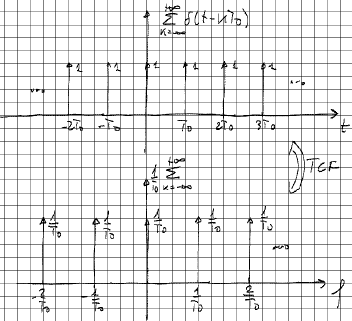
\includegraphics[width=0.65\textwidth]{treno-di-delta}
\caption{Rappresentazione grafica di un treno di delta di Dirac e della sua trasformata.}
\end{figure}

\begin{teorema}\label{th:tcf-di-segnali-periodici}
Se $y(t)$ � ottenuto per periodicizzazione dal segnale $x(t)$, allora:
\[y(t)=\sum_{k=-\infty}^{+\infty}x(t-kT_0)
   \quad\xLeftrightarrow{\TCF}\quad
  Y(f)=\frac{1}{T_0}\sum_{k=-\infty}^{+\infty}X\biggl(\frac{k}{T_0}\biggr)\delta\biggl(f-\frac{k}{T_0}\biggr).\]
\end{teorema}
\begin{proof}
\begin{align*}
Y(f) &= \int_{-\infty}^{+\infty}\sum_{k=-\infty}^{+\infty}x(t-kT_0)\e^{-\j2\pi ft}\ud t\\
     &= \sum_{k=-\infty}^{+\infty}\biggl[\int_{-\infty}^{+\infty}x(\alpha)\e^{-\j2\pi f\alpha}\ud\alpha\biggr]\e^{-\j2\pi fkT_0}\\
     &= X(f)\sum_{k=-\infty}^{+\infty}\e^{-\j2\pi fkT_0}
\intertext{avendo posto $\alpha=t-kT_0$. Applicando ora la~\eqref{eq:seconda-di-poisson-applicata-alla-delta}, ottiamo:}
Y(f) &= X(f)\frac{1}{T_0}\sum_{k=-\infty}^{+\infty}\delta\biggl(f-\frac{k}{T_0}\biggr)\\
     &= \frac{1}{T_0}\sum_{k=-\infty}^{+\infty}X(f)\bigr|_{f=k/T_0}\delta\biggl(f-\frac{k}{T_0}\biggr)\\
     &= \frac{1}{T_0}\sum_{k=-\infty}^{+\infty}X\biggl(\frac{k}{T_0}\biggr)\delta\biggl(f-\frac{k}{T_0}\biggr) =
        \sum_{k=-\infty}^{+\infty}Y_k\delta\biggl(f-\frac{k}{T_0}\biggr)
\end{align*}
si ottiene cio� in frequenza un treno di delta di Dirac pesate con dei fattori $Y_k$.
\end{proof}

\begin{figure}
\centering
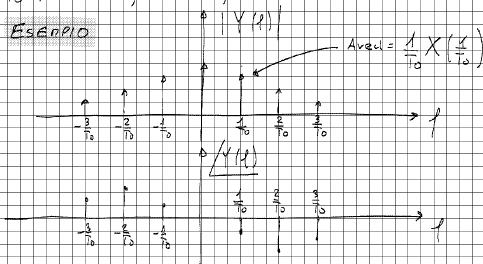
\includegraphics{tcf-di-segnali-periodocizzati}
\caption{}
\end{figure}


\subsection{Teorema di Parseval per segnali periodici}

\begin{teorema}[di Parseval per segnali periodici con \ac{TSF}]
\[\frac{1}{T_0}\int_{-\frac{T_0}{2}}^{+\frac{T_0}{2}}x(t)\,y^*(t)\ud t = \sum_{k=-\infty}^{+\infty}X_kY_k^*\]
\end{teorema}
\begin{proof}
\begin{align*}
& \frac{1}{T_0}\int_{-\frac{T_0}{2}}^{+\frac{T_0}{2}}x(t)\,y^*(t)\ud t =
        \frac{1}{T_0}\int_{-\frac{T_0}{2}}^{+\frac{T_0}{2}}\sum_{k=-\infty}^{+\infty}X_k\e^{\,\j2\pi kf_0t}\,y^*(t)\ud t\\
&\quad = \sum_{k=-\infty}^{+\infty}X_k\cdot\frac{1}{T_0}\int_{-\frac{T_0}{2}}^{+\frac{T_0}{2}}y^*(t)\e^{\,\j2\pi kf_0t}\ud t\\
&\quad = \sum_{k=-\infty}^{+\infty}X_k\biggl[\frac{1}{T_0}\int_{-\frac{T_0}{2}}^{+\frac{T_0}{2}}y(t)\e^{-\j2\pi kf_0t}\ud t\biggr]^* = \sum_{k=-\infty}^{+\infty}X_kY_k^*  \qedhere
\end{align*}
\end{proof}

Se indichiamo $x_0(t)$ e $y_0(t)$ i segnali aperiodici dai quali, per periodicizzazione, si ottengono $x(t)$ e $y(t)$:
%
\begin{align*}
x_0(t) &= x(t)\vrect(t/T_0)\\
y_0(t) &= y(t)\vrect(t/T_0)
\end{align*}
%
possiamo riscrivere il teorema di Parseval per segnali periodici utilizzando la \ac{TCF}.

\begin{teorema}[di Parseval per segnali periodici con \ac{TCF}]
\[\frac{1}{T_0}\int_{-\frac{T_0}{2}}^{+\frac{T_0}{2}}x(t)\,y^*(t)\ud t = \frac{1}{T_0^2}\sum_{k=-\infty}^{+\infty}X_0\biggl(\frac{k}{T_0}\biggr)Y_0^*\biggl(\frac{k}{T_0}\biggr)\]
\end{teorema}
\begin{proof}
La dimostrazione si ottiene applicando la relazione~\eqref{eq:relazione-trasformata-serie-continua} alla formulazione del teorema di Parseval con \ac{TSF}.
\end{proof}

Utilizzando queste due formulazioni del teorema di Parseval, si pu� scrivere la potenza media $P_x$ di un segnale periodico come:
\begin{equation}
P_x = \frac{1}{T_0}\int_{-\frac{T_0}{2}}^{+\frac{T_0}{2}}\abs{x(t)}^2\ud t = \sum_{k=-\infty}^{+\infty}\abs{X_k}^2
    = \frac{1}{T_0^2}\sum_{k=-\infty}^{+\infty}\abs{X_0\biggl(\frac{k}{T_0}\biggr)}^2.
\end{equation}

Definiamo, per il segnale periodico $x(t)$, la \emph{densit� spettrale di potenza}:
%
\[S_x(f) = \sum_{k=-\infty}^{+\infty} \frac{1}{T_0^2}\abs{X_0\biggl(\frac{k}{T_0}\biggr)}^2\delta\biggl(f-\frac{k}{T_0}\biggr).\]

\begin{teorema}
La potenza media di un segnale periodico eguaglia l'area sottesa dalla densit� spettrale di potenza:
\[P_x = \int_{-\infty}^{+\infty} S_x(f)\ud f.\]
\end{teorema}
\begin{proof}
\begin{align*}
P_x &= \int_{-\infty}^{+\infty} \sum_{k=-\infty}^{+\infty} \frac{1}{T_0^2}
       \abs{X_0\biggl(\frac{k}{T_0}\biggr)}^2\delta\biggl(f-\frac{k}{T_0}\biggr)\ud f\\
    &= \underbrace{\sum_{k=-\infty}^{+\infty} \frac{1}{T_0^2} \abs{X_0\biggl(\frac{k}{T_0}\biggr)}^2}_{P_x}
       \underbrace{\int_{-\infty}^{+\infty} \delta\biggl(f-\frac{k}{T_0}\biggr)\ud f}_{1} = P_x.  \qedhere
\end{align*}
\end{proof}


\section{Analisi energetica dei segnali aperiodici}
\label{sec:analisi-energetica-segnali-aperiodici}

La \emph{densit� spettrale di energia} di un segnale aperiodico $x(t)$ � definita come il modulo quadro della sua trasformata:
%
\[S_x(f) = \abs{X(f)}^2.\]
%
Si verifica facilmente, perci�, che l'energia media di un segnale periodico pu� essere calcolata come l'integrale della densit� spettrale di energia. La \emph{densit� spettrale di potenza} per segnali aperiodici viene definita come:
%
\[S_x(f) = \lim_{T\to\infty}\frac{\abs{X_T(f)}^2}{T}\]
%
dove $X_T(f)$ � la trasformata continua del segnale
%
\[x_T(t) = x(t)\vrect(t/T).\]
%
La potenza media � quindi l'area sottesa dalla densit� spettrale di potenza.


\paragraph{Correlazione e autocorrelazione}
Dati $x(t)$ e $y(t)$ due segnali aperiodici, si definiscono la \emph{funzione di correlazione} tra i due
%
\begin{equation}
C_{xy}(\tau) \triangleq \int_{-\infty}^{+\infty} x(t)\,y^*(t-\tau)\ud t
\end{equation}
%
e la \emph{funzione di autocorrelazione} per ciascuno di essi:
\begin{equation}
C_x(\tau) \triangleq \int_{-\infty}^{+\infty}x(t)\,x^*(t-\tau)\ud t.
\end{equation}
%
(si noti che la variabile di integrazione � $t$ mentre la variabile che caratterizza la funzione di (auto)correlazione � $\tau$). Fisicamente $\tau$ � un ritardo: per segnali reali, la funzione di autocorrelazione � l'integrale del prodotto del segnale con se stesso ritardato di un certo $\tau$.

La%
\margincomment{Questi due capoversi sono estratti dal libro~\citep[pag.~191]{b:luise} (il professore non ne ha parlato), considerando segnali reali.}
funzione di autocorrelazione fornisce informazioni utili sulla rapidit� di variazione del segnale $x(t)$. Dati due differenti segnali reali $x(t)$ e $y(t)$ aventi stessa energia ma due diverse ``velocit� di variazione'', il segnale pi� ``veloce'', supponiamo $x(t)$, presenta un valore della funzione di autocorrelazione minore di quello relativo all'altro segnale, $y(t)$, \emph{a parit� di ritardo} $\tau$. Il nome di ``autocorrelazione'' suggerisce infatti che questa funzione � un indice di ``somiglianza'' del segnale con se stesso, o meglio, con una sua replica ritardata.

Se inoltre supponiamo che il segnale $x(t)$ sia a durata rigorosamente limitata, si riesce a visualizzare immediatamente che quando la variabile $\tau$ assume valori crescenti si riduce l'ampiezza dell'intervallo in cui sia $x(t)$ che $x(t-\tau)$ assumono valori non nulli e, di conseguenza, tende a diminuire il valore di $R_x(\tau)$. Ancora, come � facilmente intuibile, il segnale $x(t)$ � massimamente correlato con se stesso per $\tau=0$, e pertanto $\abs{R_x(\tau)}\leq R_x(0)$. Infine, si ha $R_x(\tau)=R_x(-\tau)$.


\begin{proprieta}[correlazione e convoluzione]
La funzione di correlazione tra due segnali pu� essere scritta come la convoluzione tra il primo segnale e il complesso coniugato del secondo con l'asse delle ascisse invertito:
\begin{equation}
C_{xy}(\tau)=x(\tau)\otimes y^*(-\tau).
\end{equation}
\end{proprieta}
\begin{proof}
Infatti, dalla definizione di prodotto di convoluzione:
\begin{align*}
 x(\tau)\otimes y^*(-\tau) &= \int_{-\infty}^{+\infty}x(t)\,y^*(-(\tau-t))\ud t\\
                           &= \int_{-\infty}^{+\infty}x(t)\,y^*(t-\tau)\ud t=C_{xy}(\tau).  \qedhere
\end{align*}
\end{proof}

\begin{proprieta}[autocorrelazione e convoluzione]
La funzione di autocorrelazione di un segnale pu� essere scritta come la convoluzione del segnale stesso e il suo complesso coniugato con l'asse delle ascisse invertito:
\begin{equation}\label{eq:autocorrelazione-e-convoluzione}
C_x(\tau)=x(\tau)\otimes x^*(-\tau).
\end{equation}
\end{proprieta}

\begin{proprieta}
La funzione di autocorrelazione gode della propriet� di simmetria Hermitiana:
\[C_x(\tau) = C_x^*(-\tau).\]
\end{proprieta}
\begin{proof}
\begin{align*}
C_x(-\tau) & = \int_{-\infty}^{+\infty}x(t)\,x^*\bigl(t-(-\tau)\bigr)\ud t\\
           & = \int_{-\infty}^{+\infty}x(t)\,x^*(t+\tau)\ud t\\
           & = \int_{-\infty}^{+\infty}x(t'-\tau)\,x^*(t')\ud t' = C_x^*(\tau)
\end{align*}
dove � stata effettuata la sostituzione $t'=t+\tau$.
\end{proof}

\begin{lemma}
Sia dato un segnale aperiodico $x(t)$. Allora:
\begin{equation}\label{eq:trasformata-coniugato-invertito}
x^*(-t) \quad\xLeftrightarrow{\TCF}\quad X^*(f).
\end{equation}
\end{lemma}
\begin{proof}
Per la dimostrazione, basta applicare la definizione di trasformata:
\begin{align*}
 \TCF[x^*(-t)] &= \int_{-\infty}^{+\infty}x^*(-t)\e^{-\j2\pi ft}\ud t\\
               &= \int_{-\infty}^{+\infty}x^*(t')\e^{\,\j2\pi ft'}\ud t'\\
               &= \left[\int_{-\infty}^{+\infty}x(t')\e^{-\j2\pi ft'}\ud t'\right]^*=X^*(f).  \qedhere
\end{align*}
\end{proof}

\begin{proposizione}
La trasformata continua della funzione di autocorrelazione � la densit� spettrale di energia:
\[C_x(\tau) \quad\xLeftrightarrow{\TCF}\quad \abs{X(f)}^2=S_x(f).\]
\end{proposizione}
\begin{proof}
La dimostrazione pu� esser fatta molto semplicemente trasformando secondo Fourier la formula~\eqref{eq:autocorrelazione-e-convoluzione} tenendo conto della relazione~\eqref{eq:trasformata-coniugato-invertito}.
Volendo procedere tramite integrali di convoluzione:
\begin{align*}
\TCF[C_x(\tau)]
 &= \int_{-\infty}^{+\infty}C_x(\tau)\e^{-\j2\pi f\tau}\ud \tau\\
 &= \int_{-\infty}^{+\infty}\int_{-\infty}^{+\infty}x(t)\,x^*(t-\tau)\ud t \cdot\e^{-\j2\pi f\tau}\ud \tau\\
 &= \int_{-\infty}^{+\infty}x(t)\int_{-\infty}^{+\infty}x^*(t-\tau)\e^{-\j2\pi f\tau}\ud \tau \ud t\\
 &= \int_{-\infty}^{+\infty}x(t)\int_{-\infty}^{+\infty}x^*(\alpha)\e^{-\j2\pi f(t-\alpha)}\ud \alpha \ud t\\
 &= \int_{-\infty}^{+\infty}x(t)\e^{-\j2\pi ft}\ud t\cdot \int_{-\infty}^{+\infty}x^*(\alpha)\e^{\,\j2\pi f\alpha}\ud \alpha\\
 &= X(f)\left[\int_{-\infty}^{+\infty}x(\alpha)\e^{-\j2\pi f\alpha}\ud \alpha\right]^*=X(f)X^*(f)=\abs{X(f)}^2
\end{align*}
dove si � fatto il cambio di variabile $\alpha=t-\tau$.
\end{proof}

� immediato notare che la funzione di autocorrelazione calcolata in $\tau=0$ fornisce l'energia del segnale:
%
\[C_x(0) = \int_{-\infty}^{+\infty} \abs{x(t)}^2\ud t = E_x.\]
%
Si dimostra infine il seguente teorema, di fondamentale importanza.

\begin{teorema}[di Parseval]
\[\int_{-\infty}^{+\infty}x(t)\,y^*(t)\ud t=\int_{-\infty}^{+\infty}X(f)\,Y^*(f)\ud f\]
\end{teorema}
\begin{proof}
\begin{align*}
 & \int_{-\infty}^{+\infty}x(t)\,y^*(t)\ud t=
   \int_{-\infty}^{+\infty}\int_{-\infty}^{+\infty}X(f)\e^{\,\j2\pi ft}\ud f \cdot y^*(t)\ud t\\
 &\quad = \int_{-\infty}^{+\infty}X(f)\int_{-\infty}^{+\infty}y^*(t)\e^{\,\j2\pi ft}\ud t\ud f=
          \int_{-\infty}^{+\infty}X(f)\,Y^*(f)\ud f   \qedhere
\end{align*}
\end{proof}

\begin{esempio}
Calcolare l'energia del segnale:
\[x(t)=A\sinc(Bt).\]
In generale, si pu� calcolare l'energia di un segnale in due modi: a partire dall'espressione del segnale stesso o a partire dalla sua trasformata. Nel primo caso, avremmo:
\[E_x = \int_{-\infty}^{+\infty}|x(t)|^2\ud t=A^2\int_{-\infty}^{+\infty}\sinc^2(Bt)\ud t\]
che, per� non � di facile risoluzione. � conveniente invece procedere considerando la trasformata continua
\[X(f) = \frac{A}{B}\rect{f}{B}\]
ottenendo:
\[E_x = \int_{-\infty}^{+\infty}|X(f)|^2\ud f=\frac{A^2}{B^2}\int_{-\infty}^{+\infty}\rect{f}{B}\ud f=\frac{A^2}{B}.\]
\end{esempio}

% TCF_I, Teoremi_TCF, TCFG, Segnali_periodocizzati, Analisi_energetica
\chapter[Sistemi lineari stazionari a tempo continuo]{Sistemi lineari stazionari\\a tempo continuo}
\label{cha:sistemi-lineari}


\section{Sistemi}
Un sistema monodimensionale � rappresentabile con un blocco che applica una trasformazione sul segnale in ingresso
$x(t)$ per dare in uscita un segnale $y(t)$.
\begin{center}\framebox{\setlength{\unitlength}{1mm}
\begin{picture}(80,16)
\put(3,8){\vector(1,0){20}}
\put(57,8){\vector(1,0){20}}
\put(23,1){\framebox(34,14){trasformazione $\T$}}
\put(10,10){$x(t)$}
\put(63,10){$y(t)$}
\put(7,4){\mbox{ingresso}}
\put(61,4){\mbox{uscita}}
\end{picture}}\end{center}
Questa trasformazione la indichiamo con:
\begin{equation*}y(t)=\T\left[x(t)\right].\end{equation*}

Quello che faremo � caratterizzare questo tipo di sistemi e definire delle propriet� che ci torneranno utili per
dire qualcosa sull'uscita del sistema noto l'ingresso.

In generale, il valore del segnale di uscita $y$ all'istante $\bar{t}$ non dipende solo dall'ingresso $x$
all'istante $\bar{t}$ ma da $x(t)$ per $-\infty<t<\infty$.
Per poter calcolare $y(t)$ � necessario conoscere $x(t)$ su tutto l'asse del tempo, in istanti passati, presenti, futuri.

\paragraph{Linearit�.} Un sistema � lineare se � valida la sovrapposizione degli effetti. Affinch� ci� sia
verificato, a fronte di un ingresso $x(t)$ combinazione lineare di due segnali:
\begin{equation}x(t)=ax_1(t)+bx_2(t)\end{equation}
deve essere presentato in uscita il segnale:
\begin{equation}y(t)=a\T[x_1(t)]+b\T[x_2(t)]=ay_1(t)+by_2(t).\end{equation}

\paragraph{Stazionariet�.} Un sistema si dice stazionario se la sua trasformazione non cambia nel tempo (� \emph{tempo-invariante}) e applicando lo stesso ingresso a istanti diversi si ottiene esattamente la stessa uscita.

Supponiamo di avere un segnale $x(t)$ con un'uscita $y(\bar{t})$ quando l'ingresso � $x(\bar{t})$:
\[y(t) = \T[x(t)]\]
allora il sistema � stazionario se:
\begin{equation}y(t-t_0)=\T[x(t-t_0)].\end{equation}

Se in ingresso si d� il segnale $x(t)$ traslato nel tempo di $t_0$ allora in uscita si avr� semplicemente il segnale $y(t)$ traslato nel tempo di $t_0$.

\begin{figure}
\centering
\subfloat{\framebox{\begin{pspicture*}(-2.8,-1)(2.8,1.3)
  \psaxes[linewidth=0.4pt,labels=none,ticks=none]{->}(0,0)(-2.5,-0.8)(2.5,1.1)
  \psplot[linewidth=1pt,plotstyle=curve,plotpoints=200]% 0.5*sin(480*x)*\e^(-abs(x))
         {-2.2}{2.2}{0.5 x 480 mul sin mul 2.718281828459045235 x abs neg exp mul}
  \uput[l](0,0.9){$\scriptstyle{x(t)}$}
  \uput[d](2.4,0){$\scriptstyle{t}$}
\end{pspicture*}}} \quad
\subfloat{\framebox{\begin{pspicture*}(-2.8,-1)(2.8,1.3)
  \psaxes[linewidth=0.4pt,labels=none,ticks=none]{->}(0,0)(-2.5,-0.8)(2.5,1.1)
  \psplot[linewidth=1pt,plotstyle=curve,plotpoints=200]% 0.8*sin(480*x)*\e^(-abs(x))
         {-2.2}{2.2}{0.8 x 480 mul sin mul 2.718281828459045235 x abs neg exp mul}
  \uput[l](0,0.9){$\scriptstyle{\T[x(t)]}$}
  \uput[d](2.4,0){$\scriptstyle{t}$}
\end{pspicture*}}}\\
\subfloat{\framebox{\begin{pspicture*}(-2.8,-1)(2.8,1.3)
  \psaxes[linewidth=0.4pt,labels=none,ticks=none]{->}(0,0)(-2.5,-0.8)(2.5,1.1)
  \psplot[linewidth=1pt,plotstyle=curve,plotpoints=200]% 0.5*sin(480*(x-0.3))*\e^(-abs(x-0.3))
         {-2.2}{2.2}{0.5 x 0.3 sub 480 mul sin mul 2.718281828459045235 x 0.3 sub abs neg exp mul}
  \uput[l](0,0.9){$\scriptstyle{x(t-t_0)}$}
  \uput[d](2.4,0){$\scriptstyle{t}$}
\end{pspicture*}}} \quad
\subfloat{\framebox{\begin{pspicture*}(-2.8,-1)(2.8,1.3)
  \psaxes[linewidth=0.5pt,labels=none,ticks=none]{->}(0,0)(-2.5,-0.8)(2.5,1.1)
  \psplot[linewidth=1pt,plotstyle=curve,plotpoints=200]% 0.8*sin(480*(x-0.3))*\e^(-abs(x-0.3))
         {-2.2}{2.2}{0.8 x 0.3 sub 480 mul sin mul 2.718281828459045235 x 0.3 sub abs neg exp mul}
  \uput[l](0,0.9){$\scriptstyle{\T[x(t-t_0)]}$}
  \uput[d](2.4,0){$\scriptstyle{t}$}
\end{pspicture*}}}
\caption{Esemplificazione di un sistema stazionario.}
\end{figure}


\section{Sistemi lineari stazionari (\acs{SLS})}
I \acf{SLS} hanno la caratteristica di poter essere rappresentati \emph{completamente}
da una funzione $h(t)$. Il termine ``completamente'' significa che se si conosce $h(t)$ (� una funzione
del tempo) allora � possibile calcolare l'uscita $y(t)$ per un qualsiasi ingresso $x(t)$.

Per definizione:
\begin{equation}h(t)\triangleq\T\left[\delta(t)\right].\end{equation}
La funzione $h(t)$ coincide con l'uscita del sistema quando in ingresso c'� una delta di Dirac,
e infatti viene detta \emph{risposta impulsiva}.
\begin{center}\framebox{\setlength{\unitlength}{1mm}
\begin{picture}(60,10)
\put(10,5){\vector(1,0){10}}
\put(40,5){\vector(1,0){10}}
\put(20,1){\framebox(20,8){$\T[\;\cdot\;]$}}
\put(2,4){$\delta(t)$}
\put(52,4){$h(t)$}
\end{picture}}\end{center}

\begin{teorema}[uscita di un \ac{SLS}]
Per un sistema lineare e stazionario si pu� scrivere:
\[y(t)=x(t)\otimes h(t).\]
\end{teorema}
\begin{proof}
Infatti, utilizzando la propriet� di neutralit� della $\delta(t)$ nell'integrale di convoluzione, si scrive:
\begin{align*}
y(t) & = \T\left[x(t)\right]=\T\left[x(t)\otimes\delta(t)\right]\\
     & = \T\left[\int_{-\infty}^{+\infty}x(\alpha)\delta(t-\alpha)\ud\alpha\right]\\
\intertext{e siccome la trasformazione $\T[\,\cdot\,]$ e l'integrale sono entrambi operatori lineari, � possibile scambiarne l'ordine:}
     & = \int_{-\infty}^{+\infty}\T\left[x(\alpha)\delta(t-\alpha)\right]\ud\alpha.
\end{align*}

Poich� la trasformazione $\T[\,\cdot\,]$ opera rispetto al tempo, $x(\alpha)$ �, per essa, una costante. Si ha cos�:
\begin{align*}
y(t) &= \int_{-\infty}^{+\infty}x(\alpha)\T\left[\delta(t-\alpha)\right]\ud\alpha
\intertext{da cui, sfruttando l'ipotesi di stazionariet� per cui $h(t-\alpha)=\T[\delta(t-\alpha)]$, si giunge infine alla tesi:}
     & = \int_{-\infty}^{+\infty}x(\alpha)\,h(t-\alpha)\ud\alpha=x(t)\otimes h(t). \qedhere
\end{align*}
\end{proof}


\subsection{Propriet� dei \acs{SLS}}

\vspace{-\bigskipamount}%revisione
\paragraph{Causalit�.} Questa propriet� � riferibile a tutti i sistemi, non solo ai \ac{SLS}. In
generale, un sistema si dice causale quando l'uscita all'istante $\bar{t}$ dipende dal segnale
in ingresso ma solo a istanti temporali precedenti o al pi� uguali a $\bar{t}$. L'uscita, in altri,
termini deve soddisfare il principio di causa-effetto, e non pu� pertanto dipendere dall'ingresso
a istanti futuri. Tutti i sistemi fisici in natura sono sistemi causali, e un sistema che non sia causale
non � neanche fisicamente realizzabile.

Per formalizzare questo concetto, quando un \ac{SLS} � anche causale, si scrive:
\begin{equation}y(t)=\T\left[x(\alpha), \:\alpha\leq t\right].\end{equation}
Per sistemi lineari stazionari, completamente rappresentati dalla loro risposta impulsiva, si pu� controllare se siano o meno causali semplicemente guardando $h(t)$.
In particolare, un \ac{SLS} � causale se e solo se � causale sua $h(t)$, dove per $h(t)$ ``causale'' si intende nel senso di ``identicamente nulla per $t<0$'':
\begin{subequations}
\begin{align}
h(t)=0 \quad\text{per }t<0  \label{eq:h-causale-1}
\intertext{o anche:}
h(t)=h(t)\u(t).        \label{eq:h-causale-2}
\end{align}
\end{subequations}
L'impulso viene infatti applicato all'istante $t=0$ e la risposta non pu� partire prima che l'impulso sia applicato.

Proviamo a vedere cosa significa questa condizione per un qualunque segnale in ingresso.
Per quanto detto prima, l'uscita pu� essere scritta come:
\begin{align*}
y(t) &= x(t)\otimes h(t) = \int_{-\infty}^{+\infty}x(\alpha)h(t-\alpha)\ud\alpha
\intertext{e applicando la condizione di eq.~\eqref{eq:h-causale-2}, risulta:}
     &= \int_{-\infty}^{+\infty}x(\alpha)h(t-\alpha)\u(t-\alpha)\ud\alpha\\
     &= \int_{-\infty}^{t}x(\alpha)h(t-\alpha)\ud\alpha.
\end{align*}
L'integrale (e quindi l'uscita) non � influenzato dai valori dell'ingresso posteriori a $t$. Si dimostra cos� che se la risposta impulsiva di un \ac{SLS} � causale, allora � causale il \ac{SLS} stesso.
Non facciamo la dimostrazione dell'implicazione inversa, che pure potrebbe essere ottenuta ragionando per assurdo in modo analogo.

Consideriamo invece cosa accade graficamente. Supponiamo di voler calcolare $y(\bar{t})$.
%
\begin{figure}
\centering
\subfloat{\framebox{\begin{pspicture*}(-1,-0.8)(4.6,1.9)
  \psaxes[linewidth=0.4pt,labels=none,ticks=none]{->}(0,0)(-0.7,-0.6)(4.3,1.7)
  \psplot[linewidth=1pt,plotstyle=curve,plotpoints=200]% \e^(-x)
         {-0}{4}{2.718281828459045235 x neg exp}
  \uput[l](0,1.5){$\scriptstyle{h(\alpha)}$}
  \uput[d](4.2,0){$\scriptstyle{\alpha}$}
  \psline(0,0)(-0.4,0)
\end{pspicture*}}}  \quad
\subfloat{\framebox{\begin{pspicture*}(-3.2,-1)(2.4,1.7)
  \psaxes[linewidth=0.5pt,labels=none,ticks=none]{->}(0,0)(-2.9,-0.8)(2.1,1.5)
  \psplot[linewidth=1pt,plotstyle=curve,plotpoints=200]% \e^(-(t-\alpha))
         {-2.6}{0.4}{2.718281828459045235 0.4 x sub neg exp}
  \uput[l](0,1.3){$\scriptstyle{h(\bar{t}-\alpha)}$}
  \uput[d](2,0){$\scriptstyle{\alpha}$}
  \uput[d](0.4,0){$\scriptstyle{\bar{t}}$}
  \psline(0.4,0)(0.4,1)
  \psline(0.4,0)(1.8,0)
\end{pspicture*}}}\\
\subfloat{\framebox{\begin{pspicture*}(-3.8,-1.4)(3,1.7)
  \psaxes[linewidth=0.5pt,labels=none,ticks=none]{->}(0,0)(-3.5,-1.2)(2.7,1.5)
  \uput[d](2.6,0){$\scriptstyle{\alpha}$}
  \uput[d](0.4,0){$\scriptstyle{\bar{t}}$}
  \psline[linewidth=0.6pt](0.4,0)(0.4,1)
  \psplot[linewidth=0.6pt,plotstyle=curve,plotpoints=200]% \e^(-(t-\alpha))
         {-3.1}{0.4}{2.718281828459045235 0.4 x sub neg exp}
  \psplot[linewidth=0.6pt,plotstyle=curve,plotpoints=200]% cos(200*x)
         {-3.1}{2.4}{x 200 mul cos}
  \pscustom[linewidth=1pt,fillstyle=solid,fillcolor=lightgray]{%
    \psplot[linewidth=1pt,plotstyle=curve,plotpoints=200]%
           {-3.1}{0.4}{x 200 mul cos 2.718281828459045235 0.4 x sub neg exp mul}
    \psline[linewidth=0.5pt](0.4,0)(2.4,0)}
  \uput[r](1.1,-0.7){$\scriptstyle{x(\alpha)}$}
  \uput[r](0.25,1.15){$\scriptstyle{h(\bar{t}-\alpha)}$}
  \uput[u](-1,1.05){$\scriptstyle{x(\alpha)\,h(\bar{t}-\alpha)}$}
  \psline[linewidth=0.5pt]{->}(-0.9,1.1)(-0.9,-0.2)
\end{pspicture*}}}
\caption{Considerazioni grafiche per il calcolo dell'uscita di un sistema lineare stazionario: se $h()$ � nulla per $t<0$ allora il sistema � causale.}
\end{figure}
%
La $h(t)$ vale certamente $0$ per $t<0$. Il prodotto $x(\alpha)h(\bar{t}-\alpha)$ pertanto � nullo per
$\alpha>\bar{t}$, per cui $y(\bar{t})$, essendo l'integrale del prodotto, non pu� dipendere da
valori dell'ingresso $x(t)$ posteriori a $\bar{t}$.

Un sistema che produce il segnale di uscita contestualmente al segnale di ingresso � detto \emph{sistema in tempo reale}. Se invece l'uscita viene fornita dal sistema solo dopo l'acquisizione completa del segnale d'ingresso, allora si parla di \emph{sistema in tempo virtuale}. In quest'ultimo caso, si dice anche che il sistema � \emph{predittivo}.

\paragraph{Stabilit�.} Esistono diverse forme di stabilit�, noi consideriamo in particolare
quella cosiddetta \ac{BIBO}. Questo criterio afferma che a fronte di un
segnale in ingresso finito (ad ampiezza limitata), ossia tale che:
%
\[\abs{x(t)}\leq \mathrm{M} \quad\forall t\]
%
si avr� un'uscita anch'essa ad ampiezza limitata:
%
\[\abs{y(t)}\leq \mathrm{K} \quad\forall t.\]

Per sistemi lineari stazionari si pu� affermare se godano o meno della stabilit� \ac{BIBO} guardando la risposta
impulsiva.

\begin{teorema}
Un sistema lineare stazionario � stabile secondo il criterio \ac{BIBO} se e solo se la risposta impulsiva � assolutamente integrabile:
\[\int_{-\infty}^{+\infty}\abs{h(t)}\ud t=\mathrm{H}<\infty
\qquad\Leftrightarrow\qquad
\abs{y(t)}\leq\mathrm{K} \quad\forall t.\]
\end{teorema}
\begin{proof}
Consideriamo%
\margincomment{Quest'anno il Martorella ha fatto solo la dimostrazione della parte sufficiente.}
la condizione sufficiente, ossia se $h(t)$ � assolutamente integrabile allora per il sistema vale la stabilit� \ac{BIBO}. Si calcola:
\begin{align*}
\abs{y(t)} & = \abs{\int_{-\infty}^{+\infty}x(\alpha)h(t-\alpha)\ud\alpha}
               \leq\int_{-\infty}^{+\infty}\abs{x(\alpha)}\abs{h(t-\alpha)}\ud\alpha\\
\intertext{ma poich� $\abs{x(t)}\leq \mathrm{M}$ per ogni $t$}
           & \leq\mathrm{M}\int_{-\infty}^{+\infty}\abs{h(t-\alpha)}\ud\alpha=
               \mathrm{M}\int_{-\infty}^{+\infty}\abs{h(\alpha')}\ud\alpha'=\mathrm{MH}
\end{align*}
di conseguenza, l'uscita � limitata:
\begin{equation*}
\abs{y(t)} \leq \mathrm{K}, \quad \text{con }\mathrm{K}=\mathrm{MH}.
\end{equation*}

Per dimostrare la condizione necessaria (se sistema � stabile \ac{BIBO} allora la $h(t)$ � assolutamente integrabile), si consideri per assurdo che la risposta impulsiva non sia assolutamente integrabile nonostante il sistema sia stabile. Poich� il sistema � stabile (per ipotesi), dando in ingresso al sistema un segnale limitato arbitrario, il segnale di uscita corrispondente deve avere ampiezza limitata, e questo deve accadere in particolare per il segnale di ingresso (ovviamente limitato) $x(t)=\sgn\bigl(h(-t)\bigr)$ (il cosiddetto \emph{segnale del caso peggiore}). L'uscita all'istante $t=0$ vale:
\begin{align*}
y(0) &= \left.\int_{-\infty}^{+\infty}h(\alpha)\,x(t-\alpha)\ud\alpha\right|_{t=0} =
        \int_{-\infty}^{+\infty}h(\alpha)\,x(-\alpha)\ud\alpha\\
     &= \int_{-\infty}^{+\infty}h(\alpha)\sgn\bigl(h(\alpha)\bigr)\ud\alpha =
        \int_{-\infty}^{+\infty}\abs{h(\alpha)}\ud\alpha = +\infty
\end{align*}
che � un assurdo: avendo supposto per ipotesi che la risposta impulsiva del sistema non sia assolutamente integrabile, poich� il segnale di uscita non ha ampiezza limitata, il sistema in realt� non � stabile, in contraddizione con l'ipotesi fatta.
\end{proof}
\vspace{-\bigskipamount}%revisione perch� altrimenti si sommano la spaziatura per la fine proof e per il nuovo paragrafo

\paragraph{Memoria.} Nei sistemi senza memoria (detti anche istantanei), l'uscita $y(\bar{t})$ dipende solo dall'ingresso calcolato all'istante $\bar{t}$:
\[y(t)=\T\left[x(\alpha),\:\alpha=t\right].\]

I sistemi istantanei sono un caso particolare dei sistemi causali. Due segnali diversi ma coincidenti a un certo istante provocano, in quell'istante, esattamente la stessa uscita, indipendentemente dal loro andamento in tutti gli altri istanti.

I sistemi con memoria sono tutti i sistemi che non soddisfano questa condizione. Non coincidono con i sistemi causali perch� potrebbe aversi un'uscita che dipende anche dall'ingresso a istanti futuri (sistema con memoria ma non causale).

\paragraph{Invertibilit�.} Se $y(t)=\T\left[x(t)\right]$, allora il sistema si dice invertibile se
esiste una trasformazione $\T^{-1}[\:\cdot\:]$ tale che:
\[x(t)=\T^{-1}\left[y(t)\right].\]
Ovviamente non tutti i sistemi sono invertibili, ad esempio perch� esistono due ingressi che danno la
stessa uscita (ma non � questa l'unica condizione).


\section{La risposta in frequenza} D'ora in poi prenderemo in considerazione solamente i sistemi
lineari stazionari.
%
\begin{center}\framebox{\setlength{\unitlength}{1mm}
\begin{picture}(60,10)
\put(10,5){\vector(1,0){10}}
\put(40,5){\vector(1,0){10}}
\put(20,1){\framebox(20,8){$h(t)$}}
\put(2,4){$x(t)$}
\put(52,4){$y(t)$}
\end{picture}}\end{center}
%
La risposta impulsiva di un sistema potrebbe essere ricavata applicando in ingresso al sistema stesso un segnale che approssimi la funzione $\delta(t)$ e misurando l'uscita corrispondente. Il segnale $\delta(t)$ � un'astrazione matematica che pu� solo essere approssimata quando si effettua una misurazione nella pratica.
Se per� si ha un'idea dei tempi di risposta del sistema, una buona approssimazione della sollecitazione impulsiva � un impulso rettangolare di durata sufficientemente pi� piccola della costante di tempo intrinseca al sistema e di ampiezza sufficientemente elevata. Ci� che si ottiene in questo modo � la caratterizzazione del sistema nel tempo.

Spesso per� non � possibile applicare al sistema una sollecitazione impulsiva, per l'impossibilit� di generare un segnale che sia una buona approssimazione di un impulso di Dirac, ma anche perch� una sollecitazione di ampiezza elevata come l'impulso (o meglio, la sua approssimazione pratica) pu� danneggiare il sistema stesso. Cambiamo dunque tipo di eccitazione, e forniamo al sistema un segnale di ingresso sinusoidale o, meglio, per semplicit� di calcolo, un segnale nella forma:
%
\[x(t) = \e^{\,\j2\pi ft}\]
%
ossia un'oscillazione sinusoidale complessa alla frequenza $f$ (che per ora consideriamo un parametro). L'uscita corrispondente sar�:
%
\begin{align}
y(t) & = \int_{-\infty}^{+\infty}\e^{\,\j2\pi f\alpha}h(t-\alpha)\ud\alpha  \notag\\
     & = \int_{-\infty}^{+\infty}\e^{\,\j2\pi f(t-\beta)}h(\beta)\ud\beta\\
     & = \e^{\,\j2\pi ft}\int_{-\infty}^{+\infty}h(\beta)\e^{-\j2\pi f\beta}\ud\beta \notag\\
     & = x(t)\,H(f) \label{eq:relazione-ingresso-uscita-sls}
\end{align}
%
dove abbiamo posto $t-\alpha=\beta$ e definito:
%
\[H(f)\quad\xLeftrightarrow{\TCF}\quad h(t).\]

La risposta a un'oscillazione di frequenza $f$ assegnata � a sua volta un'oscillazione alla stessa frequenza $f$, ma modificata in ampiezza e fase rispetto all'ingresso di un fattore a valori complessi dipendente dalla frequenza: $H(f)$. Chiamiamo la funzione $H(f)$ \emph{risposta in frequenza} (o \emph{risposta armonica}). Poich� c'� una corrispondenza biunivoca tra risposta impulsiva e risposta in frequenza, allora anche la risposta in frequenza di un sistema lo caratterizza completamente.

Si pu�, in realt�, definire la risposta in frequenza $H(f)$ in tre modi.
%
\begin{center}\begin{tabular}{l>{$\displaystyle}l<{$}}
\toprule
Prima definizione:   & H(f)\triangleq\left.\frac{y(t)}{x(t)}\right|_{x(t)=\e^{\,\j2\pi ft}}\\
\midrule
Seconda definizione: & H(f)\triangleq\int_{-\infty}^{+\infty}h(t)\e^{-\j2\pi ft}\ud t\\
\midrule
Terza definizione:   & H(f)\triangleq\frac{Y(f)}{X(f)}\\
\bottomrule
\end{tabular}\end{center}

La prima definizione deriva dall'equazione~\eqref{eq:relazione-ingresso-uscita-sls} e consente di misurare la risposta in frequenza attraverso segnali di prova (oscillazioni a frequenza variabile). La risposta in frequenza di un sistema lineare stazionario �, cio�, data dal rapporto $y(t)/x(t)$ quando in ingresso c'� un segnale del tipo $x(t)=\e^{\,\j2\pi ft}$.

Anche la seconda definizione deriva dalla~\eqref{eq:relazione-ingresso-uscita-sls}, ed � utilizzabile quando si conosca l'andamento temporale della risposta impulsiva.

Per la terza definizione si parte invece dalla $y(t)=x(t)\otimes h(t)$ e se ne considera la trasformata
continua, ottenendo:
%
\[Y(f)=X(f)\cdot H(f)\quad\Rightarrow\quad H(f)=\frac{Y(f)}{X(f)}.\]
%
Tale relazione non pu� essere applicata a frequenze per cui si annulla lo spettro del segnale in ingresso, poich� a tali frequenze si annulla anche lo spettro dell'uscita e la risposta in frequenza risulta indeterminata. Pertanto, se la si vuole usare per determinare la $H(f)$ � necessario usare segnali in ingresso con estensione in frequenza infinita e che non si annullino mai. Se si considera $x(t)=\delta(t)$ (il cui spettro non si annulla mai: � sempre unitario), la risposta in frequenza � data proprio dallo spettro del segnale in uscita.

I vantaggi nel definire tale funzione della frequenza (la risposta in frequenza) sono nel poter capire ``al volo'' come � fatta l'uscita, anche se in termini spettrali (ad esempio capire come � fatta la banda e per quali intervalli frequenziali esiste). Noto lo spettro del segnale di ingresso e nota la risposta in frequenza del sistema, l'uscita non � altro che il loro prodotto.

\begin{esempio}
\label{es:uscita-sls}
Prendiamo in considerazione un segnale come quello rappresentato nella figura~\ref{fig:esempio-ingresso-sls}.
%
\begin{figure}[!b]
\centering
\subfloat[][Segnale di ingresso.]{\framebox{\begin{pspicture*}(-3.5,-0.6)(3.5,1.9)
  \psaxes[linewidth=0.5pt,labels=none,ticks=none]{->}(0,0)(-3.2,-0.4)(3.2,1.7)
  \uput[d](3.1,0){$f$}
  \uput[l](0,1.5){$X(f)$}
  \psplot[linewidth=1pt,plotstyle=curve,plotpoints=200]% 1*\e^(-abs(x/1.5)^2) + cos(x*550)/15
         {-2.35}{2.35}{1 2.718281828459045235 x 1.5 div abs 2 exp neg exp mul 550 x mul cos 15 div add 0.03 sub}
\end{pspicture*}}  \label{fig:esempio-ingresso-sls}}\\
\subfloat[][Risposta in frequenza.]{\framebox{\begin{pspicture*}(-3.2,-0.6)(3.2,1.9)
  \psaxes[linewidth=0.5pt,labels=none,ticks=none]{->}(0,0)(-3.0,-0.4)(2.9,1.7)
  \uput[d](2.8,0){$f$}
  \uput[l](0,1.5){$H(f)$}
  \psline[linewidth=1pt](-2.4,0)(-1.3,0)
  \psline[linewidth=0.5pt](-1.3,0)(-1.3,1)
  \psline[linewidth=1pt](-1.3,1)(1.3,1)
  \psline[linewidth=0.5pt](1.3,1)(1.3,0)
  \psline[linewidth=1pt](1.3,0)(2.4,0)
\end{pspicture*}}  \label{fig:esempio-risposta-sls}}  \quad
\subfloat[][Segnale in uscita.]{\framebox{\begin{pspicture*}(-3.2,-0.6)(3.2,1.9)
  \psaxes[linewidth=0.5pt,labels=none,ticks=none]{->}(0,0)(-3.0,-0.4)(2.9,1.7)
  \uput[d](2.8,0){$f$}
  \uput[l](0,1.5){$Y(f)$}
  \psline[linewidth=1pt](-2.4,0)(-1.3,0)
  \psline[linewidth=0.5pt](-1.3,0)(-1.3,0.52)
  \psplot[linewidth=1pt,plotstyle=curve,plotpoints=200]% 1*\e^(-abs(x/1.5)^2) + cos(x*550)/15
         {-1.3}{1.3}{1 2.718281828459045235 x 1.5 div abs 2 exp neg exp mul 550 x mul cos 15 div add 0.03 sub}
  \psline[linewidth=0.5pt](1.3,0.52)(1.3,0)
  \psline[linewidth=1pt](1.3,0)(2.4,0)
\end{pspicture*}}  \label{fig:esempio-uscita-sls}}
\caption{Esempio~\ref{es:uscita-sls}.}
\end{figure}
%
Supponiamo di volerlo trasmettere attraverso un canale trasmissivo con una certa banda (ossia che fa passare solo una certa parte del segnale). Il canale potrebbe essere un sistema lineare stazionario: lineare perch� vale il principio di sovrapposizione degli effetti (in un sistema elettrico vale sicuramente), stazionario se il canale rimane invariato (quantomeno in un certo intervallo di tempo). Se quindi il canale � lineare e stazionario allora � rappresentabile come un \ac{SLS} (figura~\ref{fig:esempio-risposta-sls}).

Per sapere come � fatto il segnale in uscita, si potrebbe considerare la risposta impulsiva del canale e fare la convoluzione con il segnale. Oppure si considera lo spettro del segnale e notando come � fatto il canale si potr� scrivere direttamente un'uscita del tipo raffigurato nella~\ref{fig:esempio-uscita-sls}.
\end{esempio}

\paragraph{Risposta in ampiezza e risposta in fase.} La risposta in frequenza di un filtro, essendo la \ac{TCF} di una funzione temporale, sar� in generale una funzione complessa e si pu� pertanto distinguere tra \emph{risposta in ampiezza} (che � il modulo della $H(f)$) e \emph{risposta in fase} (la fase di $H(f)$):
\begin{align*}
H(f) = \begin{cases}A(f)=\abs{H(f)}\\ \Phi(f)=\angle H(f).\end{cases}
\end{align*}

Le denominazioni ``risposta in ampiezza'' e ``risposta in fase'' rivelano che effettivamente, noto lo spettro del segnale di ingresso, si pu� separare il calcolo del modulo e della fase dello spettro del segnale in uscita:
\begin{align*}
Y(f) = \begin{cases}\abs{Y(f)}=\abs{X(f)}\cdot\abs{H(f)}\\ \angle Y(f)=\angle X(f)+\angle H(f).\end{cases}
\end{align*}
\vspace{-\bigskipamount}%revisione perch� altrimenti si sommano la spaziatura per la fine align e per il nuovo paragrafo

\paragraph{Decibel.} Spesso la risposta in ampiezza di segnali fisici (esempio tipico sono quelli acustici) pu� variare di molti ordini di grandezza. Si preferisce perci� rappresentarla su scala logaritmica, in decibel ($\dB$):

\begin{center}\framebox{\setlength{\unitlength}{1mm}
\begin{pspicture*}(-3.5,-0.7)(3.5,2.1)
  \psaxes[linewidth=0.5pt,labels=none,ticks=none]{->}(0,0)(-3.2,-0.1)(3.2,1.9)
  \uput[l](0,1.65){$\abs{X(f)}_{\dB}$}
  \uput[d](3.1,0){$f$}
  \infixtoRPN{1.1*2.718^(-(abs(x/1.2)^2))}
  \psplot[linewidth=0.6pt,plotstyle=curve,plotpoints=200]{-2.8}{2.8}{\RPN}
\end{pspicture*}}\end{center}
La misura in decibel dello spettro viene calcolata come:
\begin{equation}
\abs{X(f)}_{(\dB)}=10\log_{10}\abs{X(f)}.   \label{eq:decibel}
\end{equation}


\section{Risposta al gradino}

Se in ingresso a un sistema lineare stazionario si d� un gradino $\u(t)$ in uscita si ha una risposta, detta
per l'appunto ``risposta al gradino'', che viene indicata con $g(t)$:
%
\begin{figure}[b]
\centering
\framebox{\setlength{\unitlength}{1mm}
\begin{picture}(60,10)
\put(10,5){\vector(1,0){10}}
\put(40,5){\vector(1,0){10}}
\put(20,1){\framebox(20,8){$h(t)$}}
\put(2,4){$\u(t)$}
\put(52,4){$g(t)$}
\end{picture}}
\caption{La risposta al gradino $g(t)$ di un sistema lineare stazionario.}
\end{figure}
%
\begin{align*}
g(t) & = \int_{-\infty}^{+\infty}\u(\alpha)\,h(t-\alpha)\ud\alpha\\
     & = \int_{-\infty}^{+\infty}h(\beta)\u(t-\beta)\ud\beta=\int_{-\infty}^{t}h(\beta)\ud\beta.
\end{align*}
%
E pertanto:
%
\[g(t) = \int_{-\infty}^{t}h(\beta)\ud\beta  \qquad\qquad  h(t) = \frac{\ud g(t)}{\ud t}\]

Per capire l'importanza di questi risultati, consideriamo un caso pratico: torniamo al problema di misurare la risposta impulsiva di un sistema. Se ad esempio si tratta di un sistema elettrico allora bisognerebbe generare tra i due morsetti di ingresso un delta di Dirac e collegare i due morsetti di uscita a un oscilloscopio, e misurare cos� la risposta impulsiva.

In realt�, come gi� detto, non � possibile realizzare una funzione, come la delta di Dirac, che va all'infinito, ma se anche si riuscisse a farla, sicuramente si brucerebbe tutto il circuito.
Quello che si fa in pratica � mettere in ingresso un gradino o qualcosa che sale molto rapidamente (da $0$ a $1$ o da $0$ a una certa costante) e misurare quindi la risposta al gradino. Operare in tal modo � molto pi� fattibile dal punto di vista sperimentale.


\section{Collegamenti tra sistemi}
\subsection{Sistemi in cascata}
Due sistemi si dicono in cascata quando l'uscita del primo � ingresso del secondo. Un collegamento di questo tipo � rappresentato nella figura~\ref{fig:sistemi-in-cascata}.
%
\begin{figure}[b]
\centering
\framebox{\setlength{\unitlength}{1mm}
\begin{picture}(100,16)
\put(3,8){\vector(1,0){18}}
\put(41,8){\vector(1,0){18}}
\put(79,8){\vector(1,0){18}}
\put(21,2){\framebox(20,12){$h_1(t)$}}
\put(59,2){\framebox(20,12){$h_2(t)$}}
\multiput(82,15)(-2,0){33}{\line(-1,0){1}}
\multiput(83,15)(0,-2){7}{\line(0,-1){1}}
\multiput(18,1)(2,0){33}{\line(1,0){1}}
\multiput(17,1)(0,2){7}{\line(0,1){1}}
\put(5,10){$x(t)$}
\put(47,10){$y(t)$}
\put(90,10){$z(t)$}
\put(84,3){$h(t)$}
\end{picture}}
\caption{Due sistemi lineari stazionari in cascata.}
\label{fig:sistemi-in-cascata}
\end{figure}
%
Si calcola:
\begin{align*}
z(t) & = y(t)\otimes h_2(t)=\left[x(t)\otimes h_1(t)\right]\otimes h_2(t)\\
     & = x(t)\otimes\left[h_1(t)\otimes h_2(t)\right]=x(t)\otimes h(t)
\end{align*}
dove
\begin{align*}
h(t) & = h_1(t)\otimes h_2(t).
\end{align*}
Nel dominio della frequenza:
\begin{align*}
H(f) & = H_1(f)\cdot H_2(f).
\end{align*}
Due sistemi in cascata sono equivalenti a un unico sistema con risposta impulsiva data dalla convoluzione delle due
risposte impulsive e (quindi) con risposta in frequenza pari al prodotto delle risposte in frequenza dei due
sottosistemi.

\subsection{Sistemi in parallelo}
Due sistemi sono in parallelo se vengono alimentati dallo stesso ingresso e le uscite dei due vengono poi sommate.
%
\begin{figure}[t]
\centering
\framebox{\setlength{\unitlength}{1mm}
\begin{picture}(60,30)
\put(1,15){\line(1,0){10}}
\put(11,22){\line(0,-1){14}}
\put(11,8){\vector(1,0){4}}
\put(11,22){\vector(1,0){4}}
\put(35,8){\line(1,0){4}}
\put(35,22){\line(1,0){4}}
\put(39,8){\vector(0,1){5}}
\put(39,22){\vector(0,-1){5}}
\put(41,15){\vector(1,0){18}}
\put(15,16){\framebox(20,12){$h_1(t)$}}
\put(15,2){\framebox(20,12){$h_2(t)$}}
\put(39,15){\circle{4}}
\put(37.82,14.28){$\scriptstyle{+}$}
\put(2,17){$x(t)$}
\put(50,17){$y(t)$}
\put(37,24){$y_1(t)$}
\put(37,5){$y_2(t)$}
\multiput(46,29)(-2,0){19}{\line(-1,0){1}}
\multiput(47,29)(0,-2){14}{\line(0,-1){1}}
\multiput(10,1)(2,0){19}{\line(1,0){1}}
\multiput(9,1)(0,2){14}{\line(0,1){1}}
\put(48,3){$h(t)$}
\end{picture}}
\caption{Due sistemi lineari stazionari in parallelo.}
\end{figure}
%
L'uscita del sistema equivalente vale:
\begin{align*}
y(t) & = y_1(t)+y_2(t)=x(t)\otimes h_1(t)+x(t)\otimes h_2(t)\\
     & = x(t)\otimes\left[h_1(t)+h_2(t)\right]=x(t)\otimes h(t)
\end{align*}
dove
\begin{align*}
h(t) & = h_1(t)+h_2(t)
\end{align*}
e similmente
\begin{align*}
H(f) & = H_1(f)+H_2(f).
\end{align*}
Due sistemi lineari stazionari in parallelo sono equivalenti a un unico sistema con risposta impulsiva data dalla
somma delle due risposte impulsive e (quindi) con risposta in frequenza pari alla somma delle risposte in frequenza
dei due sottosistemi.


\section{Propriet� dei filtri lineari**}
\paragraph{Integrazione.}
\[w(t)=\int_{-\infty}^{t}x(\alpha)\ud\alpha\]
\begin{center}\framebox{\setlength{\unitlength}{1mm}
\begin{picture}(60,14)
\put(2,7){\vector(1,0){18}}
\put(40,7){\vector(1,0){18}}
\put(20,1){\framebox(20,12){$h(t)$}}
\put(8,9){$x(t)$}
\put(46,9){$y(t)$}
\put(8,3){$w(t)$}
\put(46,3){$z(t)$}
\end{picture}}\end{center}
\begin{align*}
w(t) & = x(t)\otimes \u(t)=\u(t)\otimes x(t)\\
z(t) & = w(t)\otimes h(t)=\left[\u(t)\otimes x(t)\right]\otimes h(t)\\
     & = \u(t)\otimes\left[x(t)\otimes h(t)\right]=\u(t)\otimes y(t)\\
     & = y(t)\otimes \u(t)=\int_{-\infty}^t y(\alpha)\ud\alpha=z(t)
\end{align*}

\paragraph{Derivazione.} La propriet� di derivazione si pu� dedurre da quella di integrazione
facendo un ragionamento inverso.
\begin{center}\framebox{\setlength{\unitlength}{1mm}
\begin{picture}(60,14)
\put(2,7){\vector(1,0){18}}
\put(40,7){\vector(1,0){18}}
\put(20,1){\framebox(20,12){$h(t)$}}
\put(8,9){$w(t)$}
\put(46,9){$z(t)$}
\put(8,3){$x(t)$}
\put(46,3){$y(t)$}
\end{picture}}\end{center}
Se
\begin{align*}w(t)=\int_{-\infty}^t x(\alpha)\ud\alpha\end{align*}
allora
\begin{align*}
x(t)=\frac{\ud w(t)}{\ud t}\quad\Rightarrow\quad y(t)=\frac{\ud z(t)}{\ud t}.
\end{align*}


\section{Filtri ideali}
\label{sec:filtri-ideali}
La teoria sui sistemi lineari stazionari si applica direttamente al problema del filtraggio dei segnali. Filtrare un segnale $x(t)$ significa trasformarlo in un altro segnale $y(t)$ avente le stesse caratteristiche di $x(t)$ (se ad esempio l'ingresso � monodimensionale e a tempo continuo, anche l'uscita lo sar�). Il sistema che effettua il filtraggio viene detto \emph{filtro}.
Ci soffermeremo in particolare sul filtraggio lineare (la trasformazione che viene fatta sul segnale � lineare), considerando sempre sistemi lineari stazionari. Un filtro quindi (per noi) non � altro che un sistema lineare stazionario, per il quale � definita una risposta impulsiva o, equivalentemente, una risposta in frequenza.

Consideriamo un segnale costituito dalla sovrapposizione di altri due segnali
\[x(t)=x_1(t)+x_2(t)\]
dei quali il primo � un segnale \emph{utile} (in quanto contiene informazioni), mentre il secondo � solo un \emph{disturbo}. Operando nel dominio del tempo non � affatto semplice eliminare il disturbo separandolo dal segnale utile. Se per� passiamo a considerare i loro spettri, pu� accadere che questi insistano su intervalli frequenziali disgiunti e che, di conseguenza, siano separabili con dei sistemi opportuni. Questi sistemi (che noi supponiamo lineari) sono per l'appunto i filtri, chiamati in questo modo proprio poich� presentano caratteristiche di \emph{selettivit�} nei confronti delle varie componenti frequenziali che compongono il segnale.

Vediamo ora dei filtri che vengono tipicamente utilizzati nelle comunicazioni. Nello specifico, vedremo solo dei filtri ideali, per cui sono definite $h(t)$ e $H(f)$ in maniera ideale, senza considerare come possono essere effettivamente realizzati.

\subsection{Passa basso}
Un filtro passa basso ideale � caratterizzato da una risposta in frequenza
\begin{align*}
H\gp{LP}(f) & = \rect{f}{2B}
\end{align*}
o equivalentemente da una risposta impulsiva
\begin{align*}
h\gp{LP}(t) & = 2B\sinc(2Bt).
\end{align*}
(Il pedice ``LP'' sta per \emph{Low Pass}.) Graficamente viene rappresentato nella figura~\ref{fig:filtro-passa-basso}.

\begin{figure}[b]
\centering
\framebox{\begin{pspicture*}(-4.3,-0.7)(4.3,1.9)
  \psaxes[linewidth=0.4pt,labels=none,ticks=none]{->}(0,0)(-4.1,-0.4)(4,1.7)
  \psline[linewidth=1pt](-1,0.8)(1,0.8)
  \psline[linewidth=0.5pt](1,0.8)(1,0)
  \psline[linewidth=0.5pt](-1,0.8)(-1,0)
  \psline[linewidth=1pt](-1,0)(-2.5,0)
  \psline[linewidth=1pt](1,0)(2.5,0)
  \psline[linewidth=1pt,linestyle=dashed,dash=2pt 2pt](-2.5,0)(-3.5,0)
  \psline[linewidth=1pt,linestyle=dashed,dash=2pt 2pt](2.5,0)(3.5,0)
  \uput[l](0,1.5){$H\gp{LP}(f)$}
  \uput[d](3.9,0){$f$}
  \uput[u](0.4,0.8){$1$}
  \uput[d](-1,0){$-B$}
  \uput[d](1,0){$+B$}
\end{pspicture*}}
\caption{Risposta in frequenza di un filtro passa passo ideale.}
\label{fig:filtro-passa-basso}
\end{figure}

Un filtro passa basso ideale lascia passare inalterate le componenti frequenziali all'interno di una certa banda (cio� intervallo di frequenze) vicino alla frequenza nulla (quindi basse frequenze). Questa zona infatti viene chiamata \emph{banda passante}, in contrapposizione alla cosiddetta \emph{banda oscura}, dove le componenti frequenziali vengono completamente eliminate. La frequenza $B$ rappresenta il cosiddetto \emph{limite di banda}. Per convenzione, $B$ � anche la \emph{banda} del filtro passa basso (pur essendo in effetti l'ampiezza della banda passante considerata solamente sul semiasse positivo delle frequenze).

\subsection{Passa banda}
La risposta in frequenza e la risposta impulsiva di un filtro passa banda sono rispettivamente:
\begin{align*}
H\gp{BP}(f) & = \rect{f-f_0}{B}+\rect{f+f_0}{B}\\
h\gp{BP}(t) & = B\sinc(Bt)\e^{\,\j2\pi f_0t}+B\sinc(Bt)\e^{-\j2\pi f_0t}\\
          & = 2B\sinc(Bt)\cos(2\pi f_0t).
\end{align*}
(Il pedice ``BP'' sta per \emph{Band Pass}.) Graficamente � rappresentato nella figura~\ref{fig:filtro-passa-banda}.
%
\begin{figure}[b]
\centering
\framebox{\begin{pspicture*}(-5.3,-0.8)(5.5,1.9)
  \psaxes[linewidth=0.4pt,labels=none,ticks=none]{->}(0,0)(-5.1,-0.4)(5.2,1.7)
  \psline[linewidth=1pt](-3,0.8)(-1,0.8)
  \psline[linewidth=1pt](-1,0)(1,0)
  \psline[linewidth=1pt](1,0.8)(3,0.8)
  \psline[linewidth=0.5pt](-3,0.8)(-3,0)
  \psline[linewidth=0.5pt](-1,0.8)(-1,0)
  \psline[linewidth=0.5pt](1,0.8)(1,0)
  \psline[linewidth=0.5pt](3,0.8)(3,0)
  \psline[linewidth=1pt](-3,0)(-4,0)
  \psline[linewidth=1pt](3,0)(4,0)
  \psline[linewidth=1pt,linestyle=dashed,dash=2pt 2pt](-4,0)(-4.8,0)
  \psline[linewidth=1pt,linestyle=dashed,dash=2pt 2pt](4,0)(4.8,0)
  \psline[linewidth=0.5pt,linestyle=dashed,dash=2pt 2pt](-1,0.8)(1,0.8)
  \uput[l](0,1.5){$H\gp{BP}(f)$}
  \uput[d](5.1,0){$f$}
  \uput[u](0.4,0.8){$1$}
  \psline[linewidth=0.5pt](-2,-0.05)(-2,0.05)
  \psline[linewidth=0.5pt](2,-0.05)(2,0.05)
  \uput[d](-2,0){$\scriptstyle{-f_0}$}
  \uput[d](2,0){$\scriptstyle{f_0}$}
  \uput[d](-3,0){$\scriptstyle{-f_0-\frac{B}{2}}$}
  \uput[d](-1,0){$\scriptstyle{-f_0+\frac{B}{2}}$}
  \uput[d](1,0){$\scriptstyle{f_0-\frac{B}{2}}$}
  \uput[d](3,0){$\scriptstyle{f_0+\frac{B}{2}}$}
\end{pspicture*}}
\caption{Risposta in frequenza di un filtro passa banda ideale.}
\label{fig:filtro-passa-banda}
\end{figure}

La frequenza $f_0$ � detta \emph{frequenza di centro banda}. La banda $B$ � definita come l'intervallo di frequenze positive dove lo spettro � non nullo. Da notare che nel filtro bassa basso l'intervallo in cui esiste la \textop{rect} � $2B$ mentre la banda � $B$, e pertanto in banda base, ovvero intorno all'origine, un filtro passa basso � di banda $B$ se la \textop{rect} va tra $-B$ e $B$. Per un passa banda, la banda � invece tutto l'intervallo della \textop{rect}.

Questi filtri sono quelli tipicamente usati per i segnali modulati emessi dalle stazioni di radiodiffusione. I vari segnali hanno infatti spettri non sovrapposti in ambito frequenziale e posti a cavallo delle cosiddette frequenze portanti su cui i radioricevitori vengono poi sintonizzati.

Per i filtri passa banda si definisce il fattore di qualit�:
\[Q\triangleq\frac{f_0}{B}.\]
Valori di $Q$ molto alti sono propri di filtri pi� \emph{selettivi}, tecnologicamente avanzati e pi� costosi. Filtri di alta qualit� hanno bande relativamente strette rispetto alla frequenza cui sono centrati. Questo rispecchia le difficolt� tecnologiche nella realizzazione di questi filtri (che possono essere pensati come un passa-basso seguito da un passa alto): un filtro di banda $B$ � pi� semplice realizzarlo a una frequenza $f_0$ piuttosto che a una frequenza (ad esempio) $10f_0$. Aumentando la frequenza $f_0$ diventa sempre pi� difficile fare filtri a banda stretta.

\subsection{Passa alto}
Il filtro passa alto (indicato con il pedice ``HP'', \emph{High Pass}) � caratterizzato dalle
seguenti relazioni:
\begin{align*}
H\gp{HP}(f) & = 1-\rect{f}{2B}\\
h\gp{HP}(t) & = \delta(t)-2B\sinc(2Bt)
\end{align*}

\begin{figure}
\centering
\framebox{\begin{pspicture*}(-5.3,-0.7)(5.5,1.9)
  \psaxes[linewidth=0.4pt,labels=none,ticks=none]{->}(0,0)(-5.1,-0.4)(5.2,1.7)
  \psline[linewidth=1pt](-4,0.8)(-1.5,0.8)
  \psline[linewidth=1pt](-1.5,0)(1.5,0)
  \psline[linewidth=1pt](1.5,0.8)(4,0.8)
  \psline[linewidth=0.5pt](-1.5,0.8)(-1.5,0)
  \psline[linewidth=0.5pt](1.5,0.8)(1.5,0)
  \psline[linewidth=1pt,linestyle=dashed,dash=2pt 2pt](-4,0.8)(-4.8,0.8)
  \psline[linewidth=1pt,linestyle=dashed,dash=2pt 2pt](4,0.8)(4.8,0.8)
  \psline[linewidth=0.5pt,linestyle=dashed,dash=2pt 2pt](-1.5,0.8)(1.5,0.8)
  \uput[l](0,1.5){$H\gp{HP}(f)$}
  \uput[d](5.1,0){$f$}
  \uput[u](0.4,0.8){$1$}
  \uput[d](-1.5,0){$-B$}
  \uput[d](1.5,0){$B$}
\end{pspicture*}}
\caption{Risposta in frequenza di un filtro passa alto ideale.}
\label{fig:filtro-passa-alto}
\end{figure}

La banda passante di un filtro passa alto � quella ``al di l�'' dell'intervallo $[-B,B]$ e la banda di un filtro passa alto, di conseguenza, � in realt� infinita. Comunque, si dice ``di banda $B$'' o ``di frequenza di taglio $B$'' per indicare il limite di banda (dove il filtro va a zero).

\subsection{Considerazioni sull'utilizzo dei filtri}
I tre filtri visti sono in effetti irrealizzabili. Consideriamo ad esempio un filtro passa basso: poich� la sua risposta impulsiva � $h\gp{LP}(t)\neq0$ per $t<0$, il filtro � non causale. Ci� significa che non � fisicamente realizzabile, e lo stesso vale per i filtri passa banda e passa alto.

Essi permettono di fare semplici operazioni sui segnali. Ad esempio, � importante avere un filtro passa banda all'uscita di un sistema di trasmissione. Infatti, il segnale da noi generato (ad esempio con la voce o musica) ha uno spettro le cui frequenze dipenderanno dalle frequenze audio della modulazione della voce o della musica. Questo spettro non � noto a priori (dipende dalla persona che parla o dalla musica che si ascolta). Al momento della trasmissione viene allocato un canale di trasmissione che potrebbe essere una banda o un intervallo di frequenze (assegnato ad esempio a una emittente radio). Questo canale ha delle caratteristiche ben precise: sar� centrato a una certa frequenza $f_0$ e avr� una certa banda. In trasmissione bisogna evitare assolutamente di trasmettere segnali con spettri che andrebbero a invadere i canali adiacenti. Per evitare questo, appena prima di arrivare all'antenna, il segnale deve passare attraverso un filtro di questo tipo che ci assicura che il segnale non fuoriesca dalla banda allocata.

Ovviamente bisogna gi� all'inizio fare in modo che il segnale stia nella banda stessa, perch� altrimenti quando lo si taglia si distrugge informazione (e modificare lo spettro del segnale significa modificare automaticamente anche il segnale stesso).

In ogni caso i filtri devono essere presenti, per non violare il sistema globale di telecomunicazione.


\section{Durata e banda}
Mentre per i filtri ideali visti nel paragrafo~\ref{sec:filtri-ideali} si � potuto definire in maniera precisa la banda, per i filtri realizzabili in pratica la differenza tra banda passante e banda oscura non � cos� netta. Per essi, come vedremo, � necessario definire la banda in maniera convenzionale.

Inoltre, il concetto di banda � estendibile anche a segnali. Dato un generico segnale $x(t)$, si definisce sullo stesso un parametro $T$ detto \emph{durata} del segnale e sul suo spettro $X(f)$ un altro parametro duale $B$ detto \emph{banda} del segnale. La durata di un segnale $x(t)$ � l'ampiezza dell'intervallo temporale all'interno del quale $x(t)$ assume valori non nulli. La banda di un segnale � l'ampiezza dell'intervallo positivo di frequenze all'interno del quale il suo spettro (di ampiezza) assume valori non nulli.

Analogamente alla banda dei filtri ``reali'' (nel senso di ``fisicamente realizzabili''), definire in maniera pratica banda e durata per i segnali non � cos� ovvio. Bisogner� trovare delle definizioni precise cui attenersi per quantificare $T$ e $B$. Diamo per ora due definizioni.

\begin{definizione}[segnale di durata rigorosamente limitata]
Si dice che un segnale $x(t)$ ha durata $T$ rigorosamente limitata se $x(t)$ ha valore arbitrario all'interno
dell'intervallo $\left[-T/2, +T/2\right]$ e identicamente nullo altrove, ossia:
\[x(t)=0 \quad\text{per } \abs{t}>T/2.\]
\end{definizione}

\begin{figure}[b!]
\centering
\subfloat{\framebox{\begin{pspicture*}(-4.3,-0.8)(4.3,2.1)
  \psaxes[linewidth=0.5pt,labels=none,ticks=none]{->}(0,0)(-4.1,-0.1)(4,1.9)
  \uput[l](0,1.65){$x(t)$}
  \uput[d](3.9,0){$t$}
  \infixtoRPN{0.4*sin(400*x)+0.33*cos(711*x)+0.32}
  \psplot[linewidth=0.6pt,plotstyle=curve,plotpoints=200]{-2.24}{2.25}{\RPN}
  \psline[linewidth=0.5pt](-2.24,-0.05)(-2.24,0.05)
  \psline[linewidth=0.5pt](2.25,-0.05)(2.25,0.05)
  \uput[d](-2.24,0){$-T/2$}
  \uput[d](2.25,0){$T/2$}
\end{pspicture*}}}\\
\subfloat{\framebox{\begin{pspicture*}(-4.3,-0.6)(4.3,1.9)
  \psaxes[linewidth=0.4pt,labels=none,ticks=none]{->}(0,0)(-4.1,-0.4)(4,1.7)
  \psline[linewidth=1pt](-1.5,1)(1.5,1)
  \psline[linewidth=0.5pt](1.5,1)(1.5,0)
  \psline[linewidth=0.5pt](-1.5,1)(-1.5,0)
  \psline[linewidth=1pt](-1.5,0)(-2.5,0)
  \psline[linewidth=1pt](1.5,0)(2.5,0)
  \psline[linewidth=1pt,linestyle=dashed,dash=2pt 2pt](-2.5,0)(-3.5,0)
  \psline[linewidth=1pt,linestyle=dashed,dash=2pt 2pt](2.5,0)(3.5,0)
  \uput[l](0,1.5){$X(f)$}
  \uput[d](3.9,0){$f$}
  \uput[d](-1.5,0){$-B$}
  \uput[d](1.5,0){$B$}
\end{pspicture*}}}
\caption{Un segnale a durata rigorosamente limitata (sopra), e un segnale a banda rigorosamente limitata (sotto).}
\end{figure}

\begin{definizione}[segnale a banda rigorosamente limitata]
Un segnale $x(t)$ si dice a banda $B$ rigorosamente limitata se ha spettro arbitrario all'interno dell'intervallo
$[-B, +B]$ e identicamente nullo altrove, ossia:
\[X(f)=0 \quad\text{per } \abs{f}>B.\]
\end{definizione}

\subsection{Relazioni tra durata e banda}
Seguono due propriet� che caratterizzano la relazione tra durata e banda di un segnale: in particolare, si pu� pensare che tra di esse sussista come una proporzionalit� inversa. Non � possibile, infatti, ridurre arbitrariamente la banda di un segnale senza aumentarne in proporzione la durata: il prodotto di queste due grandezze � \emph{limitato inferiormente}.

\begin{teorema}
Se il segnale $x(t)$ ha durata $T$ rigorosamente limitata allora il suo spettro $X(f)$ ha banda infinita.
\end{teorema}
\begin{proof}
Moltiplicando un segnale a durata rigorosamente limitata per una \textop{rect} centrata
nell'intervallo del segnale e con la stessa durata del segnale, ottengo il segnale stesso. Perci�:
\begin{align*}
X(f) & = \TCF[x(t)]=\TCF\left[x(t)\rect{t}{T}\right]\\
     & = X(f)\otimes T\sinc(Tf).
\end{align*}
Facciamo l'ipotesi (per assurdo) che $X(f)$ abbia banda rigorosamente limitata. Facendone la convoluzione con una
\textop{sinc} nel dominio della frequenza, si ottiene come risultato un segnale che ha una banda che � la somma
di quelle dei segnali originari (pu� essere intuito in modo molto semplice facendo considerazioni geometriche sul
prodotto di convoluzione). Siccome la \textop{sinc} ha componenti frequenziali fino all'infinito e quindi banda
infinita, si ottiene un segnale a banda infinita. Si arriva pertanto a dire che $X(f)$ ha banda infinita,
contraddicendo l'ipotesi iniziale.
\end{proof}

I segnali generati a partire da una voce o da una canzone hanno una certa durata. Secondo quanto appena visto,
questi segnali hanno banda infinita, e in realt� tutti i segnali che generiamo avrebbero banda infinita,
utilizzando questa definizione.
Il meccanismo usato nei sistemi di telecomunicazione di suddividere lo spettro in bande non potrebbe funzionare
(a patto di modificare il segnale stesso, con un filtro).
Dovremo definire quindi la banda in un modo pi� pratico per poter caratterizzare i vari segnali proprio in termini
di banda. � intuitivo che un segnale audio e un segnale video hanno banda diversa (e quello video ha banda molto
maggiore di quello audio), ma secondo questa definizione hanno entrambi ugualmente banda infinita.

\begin{teorema}
Se $X(f)$ � lo spettro a banda rigorosamente limitata $B$ di un segnale $x(t)$, allora $x(t)$ ha durata infinita.
\end{teorema}
\begin{proof}
La dimostrazione � analoga a quella vista nella propriet� precedente:
\begin{align*}
x(t) & = \ATCF[X(f)]=\ATCF\left[X(f)\rect{f}{2B}\right]\\
     & = x(t)\otimes 2B\sinc(2Bt).
\end{align*}
La convoluzione nel dominio del tempo tra due segnali restituisce un segnale di durata pari alla somma delle
durate dei segnali originari. Dato che la \textop{sinc} ha durata infinita anche $x(t)$ deve avere durata
infinita.
\end{proof}

Anche questa definizione, per quanto semplice, non � poi pratica.
Infatti, se si genera un segnale (a durata limitata) e lo si fa passare attraverso un filtro passa banda
ideale, si ottiene un segnale che (secondo questa definizione) ha durata infinita.


\subsection{Altre definizioni di durata e banda}
Come gi� specificato, le definizioni di durata e banda date precedentemente non sono utili in pratica.
� necessario definire una misura della durata e della banda in modo da ottenere valori finiti di entrambe.
Cos� facendo, un segnale a banda limitata potr� avere durata limitata e sar� possibile fare confronti
quantitativi tra queste grandezze di due segnali.
\begin{center}\begin{tabular}{cc}\framebox{\setlength{\unitlength}{1mm}
\begin{pspicture*}(-3,-0.8)(3,2.1)
  \psaxes[linewidth=0.5pt,labels=none,ticks=none]{->}(0,0)(-2.8,-0.1)(2.7,1.9)
  \uput[l](0,1.65){$x(t)$}
  \uput[d](2.6,0){$t$}
  \psline[linewidth=0.5pt](-1.5,0)(-1.5,0.5)
  \psplot[linewidth=0.6pt,plotstyle=curve,plotpoints=200]% 10*\e^(-abs(x/12)^2)
         {-2.3}{2.3}{1 2.718281828459045235 x 1.1 div abs 2 exp neg exp mul}
  \psline[linewidth=0.5pt](1.5,0)(1.5,0.5)
  \psline[linewidth=0.5pt]{<->}(-1.5,-0.2)(1.5,-0.2)
  \uput[d](0,-0.2){$D$}
\end{pspicture*}}&
\framebox{\setlength{\unitlength}{1mm}
\begin{pspicture*}(-3,-0.8)(3,2.1)
  \psaxes[linewidth=0.5pt,labels=none,ticks=none]{->}(0,0)(-2.8,-0.1)(2.7,1.9)
  \uput[l](0,1.65){$X(f)$}
  \uput[d](2.6,0){$f$}
  \psline[linewidth=0.5pt](-1,0)(-1,0.5)
  \psplot[linewidth=0.6pt,plotstyle=curve,plotpoints=200]% 10*\e^(-abs(x/12)^2)
         {-2.1}{2.1}{1.1 2.718281828459045235 x 0.7 div abs 2 exp neg exp mul}
  \psline[linewidth=0.5pt](1,0)(1,0.5)
  \psline[linewidth=0.5pt]{<->}(-1,-0.2)(1,-0.2)
  \uput[d](0,-0.2){$B$}
\end{pspicture*}}\end{tabular}\end{center}

\paragraph{Durata al $99$\% dell'energia.} La durata al $99$\% dell'energia viene indicata con $D_{99}$ ed � definita come l'ampiezza di quell'intervallo temporale tale che l'energia del segnale all'interno dello stesso � pari al $99\%$ dell'energia totale:
\begin{equation}
\int_{-D_{99}/2}^{+D_{99}/2}\abs{x(t)}^2\ud t=0.99 E_x
\end{equation}
Ci� equivale, in altri termini, a definire la $D_{99}$ come la durata del segnale troncato la cui energia � pari
al $99$\% dell'energia del segnale originario.


\begin{figure}[b]
\centering
\subfloat{\framebox{\begin{pspicture*}(-3.2,-0.8)(3.2,2.1)
  \psaxes[linewidth=0.5pt,labels=none,ticks=none]{->}(0,0)(-2.9,-0.1)(2.9,1.9)
  \uput[l](0,1.65){$\abs{x(t)}^2$}
  \uput[d](2.8,0){$t$}
  \infixtoRPN{1.1*2.718^(-(abs(x/1.5)^2))}
  \psplot[linewidth=0.6pt,plotstyle=curve,plotpoints=200]{-2.6}{-2}{\RPN}
  \pscustom[linewidth=1pt,fillstyle=solid,fillcolor=lightgray]{%
    \psline[linewidth=0.5pt](-2,0)(-2,0.2)
    \psplot[linewidth=0.6pt,plotstyle=curve,plotpoints=200]{-2}{2}{\RPN}
    \psline[linewidth=0.5pt](2,0.2)(2,0)}
  \psplot[linewidth=0.6pt,plotstyle=curve,plotpoints=200]{2}{2.6}{\RPN}
  \uput[r](1.1,1.4){$\scriptstyle{99\% \text{ dell'area}}$}
  \psline[linewidth=0.5pt]{->}(1.2,1.2)(0.6,0.4)
  \psline[linewidth=0.5pt]{<->}(-2,-0.2)(2,-0.2)
  \uput[d](0,-0.2){$D_{99}$}
\end{pspicture*}}} \quad
\subfloat{\framebox{\begin{pspicture*}(-3.2,-0.8)(3.2,2.1)
  \psaxes[linewidth=0.5pt,labels=none,ticks=none]{->}(0,0)(-2.9,-0.1)(2.9,1.9)
  \uput[l](0,1.65){$\abs{X(f)}^2$}
  \uput[d](2.8,0){$f$}
  \infixtoRPN{1.1*2.718^(-(abs(x)^2))}
  \psplot[linewidth=0.6pt,plotstyle=curve,plotpoints=200]{-2.6}{-1.5}{\RPN}
  \pscustom[linewidth=1pt,fillstyle=solid,fillcolor=lightgray]{%
    \psline[linewidth=0.5pt](-1.5,0)(-1.5,0.13)
    \psplot[linewidth=0.6pt,plotstyle=curve,plotpoints=200]{-1.5}{1.5}{\RPN}
    \psline[linewidth=0.5pt](1.5,0.13)(1.5,0)}
  \psplot[linewidth=0.6pt,plotstyle=curve,plotpoints=200]{1.5}{2.6}{\RPN}
  \uput[r](1,1.3){$\scriptstyle{99\% \text{ dell'area}}$}
  \psline[linewidth=0.5pt]{->}(1.1,1.1)(0.6,0.4)
  \psline[linewidth=0.5pt]{<->}(0,-0.2)(1.5,-0.2)
  \uput[d](0.75,-0.2){$B_{99}$}
\end{pspicture*}}}
\caption{Durata e banda al $99$\% dell'energia.}
\end{figure}

\paragraph{Banda al $99$\% dell'energia.} La definizione di banda al $99\%$ dell'energia viene data sfruttando il teorema di Parseval. � quel valore $B_{99}$ tale che:
\begin{equation}
\int_{-B_{99}}^{+B_{99}}\abs{X(f)}^2\ud f=0.99 E_x
\end{equation}

\paragraph{Durata a $-3\dB$ e banda a $-3\dB$.} Queste definizioni di durata e banda sono pi� utilizzate rispetto alle definizioni basate sull'energia viste precedentemente. Hanno senso per� solo per determinate tipologie di segnali. Nello specifico, si considerano trascurabili i contributi inferiori alla met� del valore massimo, ovvero quelli di $3\dB$ al di sotto del massimo su scala logaritmica.

\begin{figure}
\centering
\subfloat{\framebox{\begin{pspicture*}(-3.2,-1.2)(3.2,2.1)
  \psaxes[linewidth=0.5pt,labels=none,ticks=none]{->}(0,0)(-2.9,-0.1)(2.9,1.9)
  \uput[l](0,1.65){$\abs{x(t)}$}
  \uput[d](2.8,0){$t$}
  \infixtoRPN{1.1*2.718^(-(abs(x/1.5)^2))}
  \psline[linewidth=0.5pt](-1.25,0)(-1.25,0.55)
  \psplot[linewidth=0.6pt,plotstyle=curve,plotpoints=200]{-2.5}{2.5}{\RPN}
  \psline[linewidth=0.5pt](1.25,0.55)(1.25,0)
  \psline[linewidth=0.5pt,linestyle=dashed,dash=2pt 2pt](-0.5,1.1)(0.5,1.1)
  \uput[r](0.5,1.1){$\scriptstyle{x\gp{MAX}}$}
  \uput[r](1.25,0.55){$\scriptstyle{\frac{x\gp{MAX}}{2}}$}
  \psline[linewidth=0.5pt,linestyle=dashed,dash=2pt 2pt](-1.25,0.55)(1.25,0.55)
  \psline[linewidth=0.5pt]{<->}(-1.6,0.55)(-1.6,1.1)
  \uput[l](-1.6,0.825){$\scriptstyle{3\dB}$}
  \uput[d](-1.25,0){$\scriptstyle{t_{\mathrm{min}}}$}
  \uput[d](1.25,0){$\scriptstyle{t_{\mathrm{max}}}$}
  \psline[linewidth=0.5pt]{<->}(-1.25,-0.6)(1.25,-0.6)
  \uput[d](0,-0.6){$D_{-3\dB}$}
\end{pspicture*}}}  \quad
\subfloat{\framebox{\begin{pspicture*}(-2.7,-0.9)(3,2.4)
  \psaxes[linewidth=0.5pt,labels=none,ticks=none]{->}(0,0)(-2.4,-0.1)(2.7,1.9)
  \uput[l](0,1.65){$\abs{X(f)}$}
  \uput[d](2.6,0){$f$}
  \infixtoRPN{1.1*2.718^(-(abs(x)^2))}
  \psline[linewidth=0.5pt](-0.83,0)(-0.83,0.55)
  \psplot[linewidth=0.6pt,plotstyle=curve,plotpoints=200]{-2.1}{2.4}{\RPN}
  \psline[linewidth=0.5pt](0.83,0.55)(0.83,0)
  \psline[linewidth=0.5pt,linestyle=dashed,dash=2pt 2pt](-0.5,1.1)(0.5,1.1)
  \uput[r](0.5,1.1){$\scriptstyle{X\gp{MAX}}$}
  \uput[r](1.25,0.55){$\scriptstyle{\frac{X\gp{MAX}}{2}}$}
  \psline[linewidth=0.5pt,linestyle=dashed,dash=2pt 2pt](-0.83,0.55)(0.83,0.55)
  \uput[d](-0.83,0){$-B_{-3\dB}$}
  \uput[d](0.83,0){$B_{-3\dB}$}
\end{pspicture*}}}
\caption{Durata e banda a $-3\dB$.}
\end{figure}

La durata a $-3\dB$ (spesso detta anche ``durata a met� ampiezza'') � definita come la differenza:
\begin{equation*}
D_{-3\dB}=t_\mathrm{max}-t_\mathrm{min}
\end{equation*}
dove $t_\mathrm{min}$ e $t_\mathrm{max}$ (con $t_\mathrm{min}<t_\mathrm{max}$) sono gli istanti in cui il segnale assume in valore assoluto la met� del valore massimo $\abs{x(0)}$ e nell'intervallo $[t_\mathrm{min},t_\mathrm{max}]$ si ha $\abs{x(t)}\geq x\gp{MAX}/2$.

Se consideriamo segnali reali, per i quali la risposta in ampiezza $\abs{X(f)}$ � una funzione pari (confronta propriet�~\ref{prp:simmetria-hermitiana} a pag.~\pageref{prp:simmetria-hermitiana}), la banda a $-3\dB$ � l'ampiezza dell'intervallo di frequenze positive entro il quale lo spettro $\abs{X(f)}_{(\dB)}$ non scende di oltre $3\dB$ rispetto al suo massimo (il valore di \emph{picco}).

Considerando che
\[X(0) = X\gp{MAX} \quad\text{e}\quad X(B_{-3\dB}) = \frac{X(0)}{2} = \frac{X\gp{MAX}}{2}\]
e ragionando in termini di decibel (applicando l'eq.~\eqref{eq:decibel} a pag.~\pageref{eq:decibel}), si pu�
scrivere:
\begin{align*}
\abs{\frac{X\gp{MAX}}{2}}_{(\dB)} &= 10\log_{10}\biggl(\frac{X\gp{MAX}}{2}\biggr)\\
  &= 10\log_{10}(X\gp{MAX}) - 10\log_{10}(2)
\intertext{e poich� $10\log_{10}(2) = 3.0103\dB$, allora:}
    & \simeq \abs{X\gp{MAX}}_{(\dB)} - 3\dB.
\end{align*}
%
In definitiva:
%
\[\abs{X(B_{-3\dB})}_{(\dB)} \simeq \abs{X(0)}_{(\dB)} - 3\dB\]
ed ecco il motivo per cui la differenza tra $X\gp{MAX}$ e $X\gp{MAX}/2$ � effettivamente $3\dB$.

Come anticipato, queste definizioni non sono per� applicabili a segnali qualsiasi. Il motivo � semplice. Per un segnale con lo spettro oscillante possono essere diversi i punti in cui si incontrano i $3\dB$ al di sotto del massimo, e pertanto sarebbe un po' problematico definire la banda in questo modo. Durata e banda a $-3\dB$ hanno quindi senso solo se si hanno segnali o spettri che decrescono monotonicamente. Nella pratica, queste definizioni sono difficilmente applicabili agli usuali segnali nel tempo. Un segnale vocale, ad esempio, oscilla nel tempo molto velocemente (dipende dall'intensit� della voce, che si alza e si abbassa\dots). Sono invece generalmente applicabili purch� si ragioni in termini di banda (notare che gli spettri tipici che vengono generati dai segnali utilizzati di solito nelle telecomunicazioni sono spettri con il modulo simmetrico, perch� ottenuti da segnali reali).

Si noti che non � essenziale che intensit� del segnale o spettro decrescano monotonicamente allontanandosi dall'origine, bens� � essenziale che decrescano monotonicamente allontanandosi da una frequenza $f_0$ (per la banda) o da un istante $t_0$ (per la durata). Nell'esempio, per semplicit�, abbiamo considerato $t_0=0$ e $f_0=0$, ossia segnali e spettri cosiddetti ``passa basso''.%
\footnote{Uno spettro si dice passa-basso se la sua ampiezza assume il valore massimo per $f_0=0$. Se lo spettro � passa-alto allora $f_0=+\infty$, altrimenti lo spettro � di tipo passa-banda e $f_0$ � finita e diversa da zero.}
Per i segnali e spettri ``passa banda'', d'altronde, valgono discorsi simili, con la differenza che ad esempio lo spettro sar� centrato intorno a una certa frequenza $f_0$ e non pi� nell'origine. In tal caso, come per i filtri, il valore della banda � l'ampiezza di tutto l'intervallo (delle frequenze positive) e non la met�.

\paragraph{Banda di un \ac{SLS}.} Le definizioni date di banda valgono anche per i \ac{SLS} dove si pu� definire la $H(f)$. Ad esempio, per un filtro reale (per i quali il modulo della risposta in frequenza � una funzione pari), la banda a $-3\dB$ � l'ampiezza dell'intervallo di frequenze positive entro il quale la risposta in frequenza $\abs{H(f)}_{(\dB)}$ non scende di oltre $3\dB$ rispetto al suo massimo.


\section{Distorsioni lineari}
Trasmettere un segnale analogico senza alterarne il contenuto informativo significa ottenere
all'altro capo del sistema di comunicazione una \emph{replica fedele} del segnale originario.

\begin{definizione}[replica fedele]
Si dice che il segnale $y(t)$ � una replica fedele del segnale $x(t)$ se
\begin{equation}\label{eq:replica-fedele-nel-tempo}
y(t) = kx(t-t_0)
\end{equation}
o equivalentemente:
\begin{equation}\label{eq:replica-fedele-in-frequenza}
Y(f) = kX(f)\e^{-\j2\pi ft_0}
\end{equation}
dove $k, t_0\in\R$ e $X(f)$ e $Y(f)$ sono le traformate rispettivamente di $x(t)$ e $y(t)$.
\end{definizione}

Ci� significa che un segnale � una replica fedele di un altro se e solo se � ne una versione attenuata o
amplificata (di un valore $k$) e ritardata o anticipata (di $t_0$). La forma del segnale deve invece rimanere
la stessa.

Quando un trasmettitore invia un segnale, questo giunger� al ricevitore con un certo ritardo, dovuto alla
distanza fisica tra i due, e indebolito, perch� ovviamente non tutta la potenza trasmessa giunge al ricevitore
(anzi se ci� accadesse il ricevitore si brucerebbe subito, in quanto la potenza trasmessa � molto pi� grande di
quella che un ricevitore pu� sopportare).


\subsection{Filtro fedele}
Analizziamo ora quali sono le condizioni per un \ac{SLS} affinch� l'uscita sia una replica fedele
dell'ingresso. Queste condizioni saranno relative alla risposta impulsiva o alla risposta in frequenza.

Quando si parla di fedelt� dell'uscita, si parla anche \emph{indifferentemente} di sistemi che non introducono
distorsioni lineari. (Esistono distorsioni lineari e non lineari, ma facendo riferimento a sistemi lineari
ci si riferisce sempre alle prime, in quanto un \ac{SLS} non pu� introdurre distorsioni non lineari.)

\pagebreak%revisione
Per un sistema lineare stazionario:
\begin{center}\framebox{\setlength{\unitlength}{1mm}
\begin{picture}(60,10)
\put(10,5){\vector(1,0){10}}
\put(40,5){\vector(1,0){10}}
\put(20,1){\framebox(20,8){$h(t)$}}
\put(2,4){$x(t)$}
\put(52,4){$y(t)$}
\end{picture}}\end{center}
il segnale di uscita $y(t)$ � una versione non distorta dell'ingresso $x(t)$ se ne differisce solo per una costante moltiplicativa e un ritardo:
\begin{equation}\label{eq:y-non-distorta}
y(t) = k\,x(t-t_0).
\end{equation}

Nel caso pi� generale, affinch� ci� si verifichi la risposta impulsiva $h(t)$ deve essere nella forma:
\begin{equation}\label{eq:h-non-distorcente}
h(t)=k\delta(t-t_0)
\end{equation}
Infatti, facendone la convoluzione con l'ingresso $x(t)$ si ottiene esattamente il segnale di eq.~\eqref{eq:y-non-distorta}. Questa condizione si traduce nel dominio della frequenza nella:
\begin{equation}\label{eq:H-non-distorcente}
H(f)=k\e^{-\j2\pi ft_0}
\end{equation}
come ci si poteva aspettare facendo il rapporto tra ingresso e uscita nella eq.~\eqref{eq:replica-fedele-in-frequenza}.
In termini di ampiezza di spettro e di fase risulta:
\begin{equation*}
\abs{H(f)} = \abs{k}  \quad\text{e}\quad  \angle H(f) = -2\pi ft_0 + \angle k
\end{equation*}
(dove si tiene conto di modulo e fase di $k$ in quanto in generale $k$ pu� essere un reale sia positivo che negativo: $\angle k=0$ se $k\in\R^+_0$, e $\angle k=\pi$ se $k\in\R^-$).
Per un filtro fedele, il modulo della risposta in frequenza deve essere costante su tutto l'asse delle frequenze (un filtro con una risposta in ampiezza di questo tipo passa tutto), mentre la risposta in fase deve essere lineare con la frequenza (in termini temporali corrisponde a un ritardo). Se non � rispettata la condizione sulla risposta in ampiezza, si dice che il segnale in ingresso subisce \emph{distorsione di ampiezza}; se invece non � rispettata la condizione sulla risposta in fase, si dice che il segnale subisce \emph{distorsione di fase}.

I sistemi lineari che soddisfano la condizione di eq.~\eqref{eq:h-non-distorcente} o la \eqref{eq:H-non-distorcente} non introducono mai distorsioni lineari. Ci� non significa che i sistemi che non le soddisfano introducano sempre distorsioni lineari: � sufficiente che siano soddisfatte solo alle frequenze in cui � presente lo spettro del segnale in ingresso. Ad esempio, i filtri tipici gi� visti (passa alto, passa basso e passa banda) non sono, in generale, filtri fedeli, ma in generale non lo � nessun filtro fisico, non potendo garantire una risposta in ampiezza costante su tutto l'asse delle frequenze. In realt�, per sapere se un filtro introduce effettivamente distorsioni bisogna conoscere il segnale di ingresso, e nulla si pu� dire a priori.

\begin{esempio}
\label{es:esempio-distorsioni-lineari}
Consideriamo il segnale rappresentato nella figura~\ref{fig:esempio-distorsioni-lineari}.
%
\begin{figure}
\centering
\subfloat[Segnale dell'esempio~\ref{es:esempio-distorsioni-lineari}.]{\framebox{\begin{pspicture*}(-4,-0.7)(4,1.9)
  \psaxes[linewidth=0.4pt,labels=none,ticks=none]{->}(0,0)(-3.7,-0.4)(3.7,1.7)
  \psline[linewidth=1pt](-1.8,0)(0,1)
  \psline[linewidth=1pt](1.8,0)(0,1)
  \uput[d](-1.8,0){$-B$}
  \uput[d](1.8,0){$+B$}
  \uput[l](0,1.5){$X(f)$}
  \uput[d](3.6,0){$f$}
\end{pspicture*}}  \label{fig:esempio-distorsioni-lineari}}\\
\subfloat{\framebox{\begin{pspicture*}(-2.7,-0.7)(3.3,1.9)
  \psaxes[linewidth=0.4pt,labels=none,ticks=none]{->}(0,0)(-2.5,-0.4)(3,1.7)
  \psline[linewidth=1pt](-1.8,0.8)(1.8,0.8)
  \psline[linewidth=0.5pt,linestyle=dashed,dash=2pt 2pt](-1.8,0)(-1.8,0.8)
  \psline[linewidth=0.5pt,linestyle=dashed,dash=2pt 2pt](1.8,0)(1.8,0.8)
  \uput[d](-1.8,0){$-B$}
  \uput[d](1.8,0){$+B$}
  \uput[r](0,1.5){$\abs{H_1(f)}$}
  \uput[d](2.9,0){$f$}
\end{pspicture*}}} \quad
\subfloat{\framebox{\begin{pspicture*}(-2.7,-1.2)(3.3,1.4)
  \psaxes[linewidth=0.4pt,labels=none,ticks=none]{->}(0,0)(-2.5,-0.9)(3,1.2)
  \psline[linewidth=1pt](-1.8,0.8)(1.8,-0.8)
  \psline[linewidth=0.5pt,linestyle=dashed,dash=2pt 2pt](-1.8,0)(-1.8,0.8)
  \psline[linewidth=0.5pt,linestyle=dashed,dash=2pt 2pt](1.8,0)(1.8,-0.8)
  \uput[d](-1.8,0){$-B$}
  \uput[u](1.8,0){$+B$}
  \uput[r](0,1){$\angle H_1(f)$}
  \uput[d](2.9,0){$f$}
\end{pspicture*}}}\\
\subfloat{\framebox{\begin{pspicture*}(-2.7,-0.7)(3.3,1.9)
  \psaxes[linewidth=0.4pt,labels=none,ticks=none]{->}(0,0)(-2.5,-0.4)(3,1.7)
  \psline[linewidth=1pt](-0.9,0.8)(0.9,0.8)
  \psline[linewidth=0.5pt,linestyle=dashed,dash=2pt 2pt](-0.9,0)(-0.9,0.8)
  \psline[linewidth=0.5pt,linestyle=dashed,dash=2pt 2pt](0.9,0)(0.9,0.8)
  \uput[d](-0.9,0){$-B/2$}
  \uput[d](0.9,0){$+B/2$}
  \uput[r](0,1.5){$\abs{H_2(f)}$}
  \uput[d](2.9,0){$f$}
\end{pspicture*}}} \quad
\subfloat{\framebox{\begin{pspicture*}(-2.7,-1.2)(3.3,1.4)
  \psaxes[linewidth=0.4pt,labels=none,ticks=none]{->}(0,0)(-2.5,-0.9)(3,1.2)
  \psline[linewidth=1pt](-1.8,-0.8)(1.8,0.8)
  \psline[linewidth=0.5pt,linestyle=dashed,dash=2pt 2pt](-1.8,0)(-1.8,-0.8)
  \psline[linewidth=0.5pt,linestyle=dashed,dash=2pt 2pt](1.8,0)(1.8,0.8)
  \uput[u](-1.8,0){$-B$}
  \uput[d](1.8,0){$+B$}
  \uput[r](0,1.0){$\angle H_2(f)$}
  \uput[d](2.9,0){$f$}
\end{pspicture*}}}\\
\subfloat{\framebox{\begin{pspicture*}(-2.7,-0.7)(3.3,1.9)
  \psaxes[linewidth=0.4pt,labels=none,ticks=none]{->}(0,0)(-2.5,-0.4)(3,1.7)
  \psline[linewidth=1pt](-1.8,0.8)(1.8,0.8)
  \psline[linewidth=0.5pt,linestyle=dashed,dash=2pt 2pt](-1.8,0)(-1.8,0.8)
  \psline[linewidth=0.5pt,linestyle=dashed,dash=2pt 2pt](1.8,0)(1.8,0.8)
  \uput[d](-1.8,0){$-B$}
  \uput[d](1.8,0){$+B$}
  \uput[r](0,1.5){$\abs{H_3(f)}$}
  \uput[d](2.9,0){$f$}
\end{pspicture*}}}  \quad
\subfloat{\framebox{\begin{pspicture*}(-2.7,-1.2)(3.3,1.4)
  \psaxes[linewidth=0.4pt,labels=none,ticks=none]{->}(0,0)(-2.5,-0.9)(3,1.2)
  \psplot[linewidth=1pt,plotstyle=curve,plotpoints=200]%
        {-1.8}{1.8}{0.5 x 100 mul sin mul}
  \uput[u](-1.8,0){$-B$}
  \uput[d](1.8,0){$+B$}
  \uput[r](0,1.0){$\angle H_3(f)$}
  \uput[d](2.9,0){$f$}
\end{pspicture*}}}\\
\subfloat{\framebox{\begin{pspicture*}(-2.7,-0.7)(3.3,1.9)
  \psaxes[linewidth=0.4pt,labels=none,ticks=none]{->}(0,0)(-2.5,-0.4)(3,1.7)
  \psline[linewidth=1pt](-1.8,1)(0,0)
  \psline[linewidth=1pt](0,0)(1.8,1)
  \psline[linewidth=0.5pt,linestyle=dashed,dash=2pt 2pt](-1.8,0)(-1.8,1)
  \psline[linewidth=0.5pt,linestyle=dashed,dash=2pt 2pt](1.8,0)(1.8,1)
  \uput[d](-1.8,0){$-B$}
  \uput[d](1.8,0){$+B$}
  \uput[r](0,1.5){$\abs{H_4(f)}$}
  \uput[d](2.9,0){$f$}
\end{pspicture*}}} \quad
\subfloat{\framebox{\begin{pspicture*}(-2.7,-1.2)(3.3,1.4)
  \psaxes[linewidth=0.4pt,labels=none,ticks=none]{->}(0,0)(-2.5,-0.9)(3,1.2)
  \psline[linewidth=1pt](-1.8,0.8)(0,-0.6)
  \psline[linewidth=1pt](0,0.6)(1.8,-0.8)
  \psline[linewidth=0.5pt,linestyle=dashed,dash=2pt 2pt](-1.8,0)(-1.8,0.8)
  \psline[linewidth=0.5pt,linestyle=dashed,dash=2pt 2pt](1.8,0)(1.8,-0.8)
  \uput[d](-1.8,0){$-B$}
  \uput[u](1.8,0){$+B$}
  \uput[r](0,1.0){$\angle H_4(f)$}
  \uput[d](2.9,0){$f$}
\end{pspicture*}}}
\caption{Esempio~\ref{es:esempio-distorsioni-lineari}.}
\end{figure}
\end{esempio}

Un filtro come $H_1(f)$ non distorce il segnale~\ref{fig:esempio-distorsioni-lineari}, in quanto l'ampiezza � costante nell'intervallo frequenziale all'interno del quale esiste il segnale di ingresso e la fase � lineare con la frequenza ($t_0>0$).
Il filtro $H_2(f)$ introduce invece distorsioni di ampiezza, in quanto la sua risposta in ampiezza non � costante
su tutto l'intervallo in cui il segnale in ingresso possiede componenti frequenziali.
Al contrario si comporta il filtro $H_3(f)$, che introduce invece distorsioni di fase, ma non distorsioni di ampiezza.
L'ultimo filtro, $H_4(f)$, introduce distorsioni sia di ampiezza che di fase.


\section{Filtraggio di segnali periodici}

Come gi� dimostrato (vedi teorema~\ref{th:tcf-di-segnali-periodici} a pagina~\pageref{th:tcf-di-segnali-periodici}), la trasformata continua di un segnale periodico � costituita da una successione di impulsi di area pari ai coefficienti della serie di Fourier. Facendo riferimento alla seguente figura
%
\begin{center}\framebox{\setlength{\unitlength}{1mm}
\begin{picture}(60,10)
\put(10,5){\vector(1,0){10}}
\put(40,5){\vector(1,0){10}}
\put(20,1){\framebox(20,8){$h(t)$}}
\put(2,4){$x(t)$}
\put(52,4){$y(t)$}
\end{picture}}\end{center}
%
supponiamo che $x(t)$ sia un segnale periodico. Allora l'uscita �:
%
\[Y(f) = X(f)H(f)=\sum_{k=-\infty}^{+\infty} X_k\delta\biggl(f-\frac{k}{T_0}\biggr)H(f).\]
%
Se $H(f)$ � (per esempio) un filtro passa basso ideale, allora in uscita saranno riportati solamente alcuni degli impulsi presenti nell'ingresso.

\begin{figure}[b!]
\centering
\subfloat{\framebox{\setlength{\unitlength}{1mm}
 \begin{picture}(60,25)(-27,-5)
 \put(0,-1){\vector(0,1){18}}
 \put(-25,0){\vector(1,0){52}}
 \put(2,16){$X(f)$}
 \put(28,-1){$f$}
 \put(-25,-4){$\scriptstyle{-\frac{3}{T_0}}$}
 \put(-17,-4){$\scriptstyle{-\frac{2}{T_0}}$}
 \put(-9,-4){$\scriptstyle{-\frac{1}{T_0}}$}
 \put(4,-4){$\scriptstyle{+\frac{1}{T_0}}$}
 \put(12,-4){$\scriptstyle{+\frac{2}{T_0}}$}
 \put(20,-4){$\scriptstyle{+\frac{3}{T_0}}$}
 \thicklines
 \put(-21,0){\vector(0,1){3}}
 \put(-14,0){\vector(0,1){5}}
 \put(-7,0){\vector(0,1){8}}
 \put(0,0){\vector(0,1){12}}
 \put(7,0){\vector(0,1){8}}
 \put(14,0){\vector(0,1){5}}
 \put(21,0){\vector(0,1){3}}
 \end{picture}}} \quad
\subfloat{\framebox{\setlength{\unitlength}{1mm}
 \begin{picture}(50,25)(-22,-5)
 \put(0,-1){\vector(0,1){14}}
 \put(-20,0){\vector(1,0){42}}
 \put(-5,16){$H(f)$}
 \put(23,-1){$f$}
 \put(2,10){$1$}
 \put(-16,-4){$-\frac{3}{2T_0}$}
 \put(10,-4){$+\frac{3}{2T_0}$}
 \put(-13,0){\line(0,1){8}}
 \put(13,0){\line(0,1){8}}
 \thicklines
 \put(-13,8){\line(1,0){26}}
 \end{picture}}}  \\ 
\subfloat{\framebox{\setlength{\unitlength}{1mm}
 \begin{picture}(60,25)(-27,-5)
 \put(0,-1){\vector(0,1){18}}
 \put(-25,0){\vector(1,0){52}}
 \put(2,16){$Y(f)$}
 \put(28,-1){$f$}
 \put(-13,-4){$-\frac{1}{T_0}$}
 \put(8,-4){$+\frac{1}{T_0}$}
 \thicklines
 \put(-10,0){\vector(0,1){8}}
 \put(0,0){\vector(0,1){12}}
 \put(10,0){\vector(0,1){8}}
\end{picture}}}
\caption{Il filtraggio di un segnale periodico fornisce in uscita un segnale anch'esso periodico.}
\end{figure}
%
Si pu� dimostrare che il segnale in uscita a un filtro lineare quando in ingresso � presente un segnale periodico � ancora un segnale periodico.

Uno
\annotation{}{Queste sono considerazioni mie.}%
spettro continuo $X(f)$ costituito da sole delta di Dirac corrisponde nel tempo a una somma di oscillazioni esponenziali complesse. Se tutte queste oscillazioni hanno frequenze multiple di una frequenza fondamentale, allora il segnale risultante � periodico. Infatti, una somma di due segnali periodici � ancora un segnale periodico solamente se il rapporto $f_1/f_2$ tra le frequenze dei due segnali di partenza � un numero razionale. Poich� un filtro lineare pu� solamente modificare in ampiezza o tagliare impulsi in ingresso, ma non aggiungerne, se in ingresso si ha un segnale periodico allora certamente le delta sono posizionate in frequenze multiple di una frequenza fondamentale $f_0$, quindi anche gli impulsi riportati in uscita lo sono. Di conseguenza il segnale in uscita � periodico.


\section{Filtri e analisi energetica}

Vogliamo, ora, trovare dei metodi che consentano di fare valutazioni energetiche sul segnale in uscita senza dover calcolare il segnale di uscita stesso (in funzione del tempo o della frequenza).
Due importanti parametri energetici sono la funzione di autocorrelazione e la densit� spettrale di energia.
%
\begin{center}\framebox{\setlength{\unitlength}{1mm}
\begin{picture}(60,10)
\put(10,5){\vector(1,0){10}}
\put(40,5){\vector(1,0){10}}
\put(20,1){\framebox(20,8){$h(t)$}}
\put(2,4){$x(t)$}
\put(52,4){$y(t)$}
\end{picture}}\end{center}
%
Ad esempio, noto il segnale in ingresso anche solo tramite la sua funzione di autocorrelazione o la sua densit� spettrale di energia, � possibile ottenere informazioni sul segnale di uscita quali la sua funzione di autocorrelazione e la sua densit� di energia.


\subsection{Segnali aperiodici}
\label{sec:filtraggio-segnali-aperiodici}

Richiamiamo brevemente alcuni concetti relativi agli aspetti energetici di segnali aperiodici.
Dati due segnali a energia finita $x(t)$ e $y(t)$, sono definite le rispettive \emph{funzioni di autocorrelazione}, ciascuna scrivibile come convoluzione tra il segnale stesso e il suo complesso coniugato con l'asse delle ascisse invertito:
\begin{align*}
R_x(\tau) &= x(\tau)\otimes x^*(-\tau)\\
R_y(\tau) &= y(\tau)\otimes y^*(-\tau).
\end{align*}
%
Inoltre, la \ac{TCF} della funzione di autocorrelazione � la \emph{densit� spettrale di energia}:
%
\begin{align*}
\TCF[R_x(\tau)] &= X(f)\,X^*(f) = \abs{X(f)}^2 = S_x(f).
\end{align*}

Giungiamo ora a dimostrare un risultato molto importante, che ci consente di fare valutazioni energetiche
relativamente al segnale di uscita senza conoscere il segnale di uscita stesso.

\begin{teorema}
La funzione di autocorrelazione del segnale in uscita vale:
\[R_y(\tau)=R_x(\tau)\otimes h(\tau)\otimes h^*(-\tau).\]
\end{teorema}
\begin{proof}
La dimostrazione, anzich� farla nel dominio del tempo (bisognerebbe trattare tre integrali di convoluzione), la si fa sfruttando la \ac{TCF}. Si considera inizialmente la densit� spettrale di energia del segnale in uscita, che �:
\begin{align*}
S_y(f) & = \abs{Y(f)}^2 = \abs{X(f)}^2\cdot\abs{H(f)}^2=S_x(f)\,H(f)\,H^*(f)
\end{align*}
e antitrasformando si ottiene la tesi.
\end{proof}

\subsection{Segnali periodici**}
I segnali aperiodici che abbiamo considerato hanno energia finita e potenza nulla. I segnali periodici, invece, hanno energia infinita e potenza finita. Per questo motivo, essi vanno caratterizzati sulla base della potenza e non pi� dell'energia.

Come gi� visto, se si pone in ingresso a un \ac{SLS} un segnale periodico, anche in uscita ci sar� un segnale periodico (questo � garantito, in particolare, dall'ipotesi di stazionariet� del sistema, non di linearit�). Per tale motivo la definizione della funzione di autocorrelazione si applica sia al segnale in ingresso che a quello in uscita:
\begin{equation}
 R_x(\tau)\triangleq\frac{1}{T_0}\int_{-\frac{T_0}{2}}^{+\frac{T_0}{2}}x(t)\,x^*(t-\tau)\ud t
\end{equation}
\begin{equation}
 R_y(\tau)\triangleq\frac{1}{T_0}\int_{-\frac{T_0}{2}}^{+\frac{T_0}{2}}y(t)\,y^*(t-\tau)\ud t.
\end{equation}

Per segnali periodici, la funzione di autocorrelazione calcolata in $\tau=0$ restituisce la potenza media del
segnale:
\begin{align*}
\left.R_x(\tau)\right|_{\tau=0}=R_x(0)=\frac{1}{T_0}\int_{-\frac{T_0}{2}}^{+\frac{T_0}{2}}x(t)\,x^*(t)\ud t=P_x
\end{align*}

\begin{teorema}
La funzione di autocorrelazione del segnale in uscita vale:
\[R_y(\tau)=R_x(\tau)\otimes h(\tau)\otimes h(-\tau).\]
\end{teorema}
\begin{proof}
La \annotation[caption={Autocorrelazione di segnali periodici.}]{dimostrazione}{Vedere sul libro il paragrafo 4.4 e il sommario a pagina 212-213. Che senso ha usare la \ac{TCF} se ho definito $R_x(\tau)$ e $R_y(\tau)$ per segnali periodici come integrali sul periodo?} � analoga a quella fatta per i segnali aperiodici.
\begin{align*}
S_y(f) & = \abs{X(f)}^2\cdot\abs{H(f)}^2=
           \sum_{k=-\infty}^{+\infty}\abs{X_k}^2\delta\left(f-\frac{k}{T_0}\right)\abs{H(f)}^2\\
       & = S_x(f)H(f)H^*(f)
\end{align*}
Antitrasformando, otteniamo la tesi.
\end{proof}


\subsection{Segnali aperiodici a potenza finita*}
\begin{align*}
R_x(\tau) & = \lim_{T\to\infty}\frac{1}{T}\int_{-\frac{T}{2}}^{+\frac{T}{2}}x(t)x^*(t-\tau)\ud t & \\
S_x(f) & = \lim_{T\to\infty}\frac{1}{T}\abs{X_T(f)}^2\\
 & X_T(f)=\TCF\big[x_T(t)\big] \qquad\qquad x_T(t) = x(t)\rect{t}{T}
\end{align*}
\[R_y(\tau)=R_x(\tau)\otimes h(\tau)\otimes h(-\tau)\]


% !TeX encoding = ISO-8859-1
% !TeX root = appunti.tex

\chapter[Sistemi non lineari a tempo continuo]{Sistemi non lineari\\a tempo continuo}
\label{cha:sistemi-non-lineari}


\section{Concetti generali}
I sistemi non lineari sono per definizione tutti quei sistemi che non soddisfano la condizione di linearit�.
Essi sono il risultato di due tipi di non linearit�:
\begin{itemize}
\item \emph{non linearit� essenziali} che sono non linearit� volute che risultano essenziali per il corretto
      funzionamento di un sistema;
\item \emph{non linearit� parassite} che sono invece non linearit� non volute, sono spurie, legate a problemi di
      costruzione di sistemi che si vorrebbero lineari (\emph{nominalmente lineari}) ma non lo sono completamente.
\end{itemize}
Vediamo alcuni esempi.

\paragraph{Quadratore.}
Il quadratore � un esempio classico di non linearit� essenziale. Fornisce in uscita il quadrato dell'ingresso e viene utilizzato in particolare per raddoppiare la frequenza di un'oscillazione.
%
\begin{center}\makebox[\textwidth][s]{\hspace{1cm}
 \begin{minipage}{0.25\textwidth}$\displaystyle{y(t)=x^2(t)}$\end{minipage}
 \begin{minipage}{0.55\textwidth}
  \begin{flushright}\framebox{\setlength{\unitlength}{1mm}\begin{picture}(60,10)
  \put(10,5){\vector(1,0){10}}
  \put(40,5){\vector(1,0){10}}
  \put(20,1){\framebox(20,8){$(\:\cdot\:)^2$}}
  \put(2,4){$x(t)$}
  \put(52,4){$y(t)$}
 \end{picture}}\end{flushright}
 \end{minipage}
 \hspace{1cm}}\end{center}

\paragraph{Amplificatore non ideale.}
Un amplificatore ideale con un guadagno pari ad $A$ � caratterizzato dalla relazione ingresso-uscita
%
\[y(t)=Ax(t).\]
%
Ma tutti gli amplificatori reali introducono delle distorsioni, che vengono rappresentate tramite un
termine $d(t)$.
%
\begin{center}\makebox[\textwidth][s]{\hspace{1cm}
 \begin{minipage}{0.35\textwidth}$\displaystyle{y(t)=Ax(t)+d(t)}$\end{minipage}
 \begin{minipage}{0.45\textwidth}
  \begin{flushright}\framebox{\setlength{\unitlength}{1mm}\begin{picture}(50,14)
   \put(10,7){\vector(1,0){9}}
   \put(31,7){\vector(1,0){9}}
   \put(19,13){\line(0,-1){12}}
   \put(19,13){\line(2,-1){12}}
   \put(19,1){\line(2,1){12}}
   \put(21,6){$A$}
   \put(2,6){$x(t)$}
   \put(42,6){$y(t)$}
  \end{picture}}\end{flushright}
 \end{minipage}
 \hspace{1cm}}\end{center}
 
Peraltro, entro un certo intervallo di valori dell'ingresso l'amplificatore pu� supportare l'uscita correttamente amplificata,  ma all'esterno dell'intervallo stesso si giunge a una situazione di saturazione, per cui l'uscita non supera un valore limite (introducendo cos� ulteriori distorsioni non lineari).

Notare che queste distorsioni sono completamente diverse da quelle lineari (introdotte dai sistemi lineari).
I sistemi lineari non introducono distorsioni lineari se e solo se generano in uscita una replica fedele del segnale
in ingresso. Per sistemi non lineari, invece, non vale la mutua esclusione tra distorsione e replica
fedele.

\begin{center}\framebox{\setlength{\unitlength}{1mm}
\begin{picture}(60,10)
\put(10,5){\vector(1,0){10}}
\put(40,5){\vector(1,0){10}}
\put(20,1){\framebox(20,8){$\text{\textsc{snl}}$}}
\put(2,4){$x(t)$}
\put(52,4){$y(t)$}
\end{picture}}\end{center}

Prenderemo in considerazione sistemi non lineari monodimensionali a tempo continuo e in particolare quelli \emph{stazionari} e \emph{senza memoria}. Tali sistemi si possono descrivere molto semplicemente tramite la propria \emph{caratteristica ingresso-uscita}, che � una semplice funzione rappresentabile graficamente su un piano cartesiano con l'ingresso e l'uscita sui due assi:

\begin{center}\framebox{\setlength{\unitlength}{1mm}
\begin{pspicture*}(-4.3,-1.3)(4.3,1.6)
  \psaxes[linewidth=0.5pt,labels=none,ticks=none]{->}(0,0)(-4.1,-1.1)(4,1.4)
  \uput[l](0,1.2){$y$}
  \uput[d](3.9,0){$x$}
  \psplot[linewidth=0.6pt,plotstyle=curve,plotpoints=200]{-2}{0}{x 2 div 2 exp neg}
  \psplot[linewidth=0.6pt,plotstyle=curve,plotpoints=200]{0}{2}{x 2 div 2 exp}
\end{pspicture*}}\end{center}
%
Notare che il tempo non � rappresentato, dato che il sistema � istantaneo e stazionario e la $t$
non influisce sull'uscita.

Per i sistemi non lineari non ha senso definire una risposta impulsiva. L'uscita da un sistema non lineare si pu� ottenere tramite la caratteristica ingresso-uscita \textop{g}:
%
\[y(t)=\operatorname{g}[x(t)].\]


\section{Non linearit� essenziali}
Molti sistemi non lineari vengono utilizzati per realizzare componenti di sistemi complessi. Infatti, hanno la caratteristica di produrre contributi frequenziali nel segnale di uscita che non erano presenti nel segnale di ingresso e questo viene sfruttato per realizzare, ad esempio, i raddrizzatori a doppia semionda ($g(x)=\abs{x}$) dei circuiti alimentatori degli apparati elettronici, o i moltiplicatori di frequenza.

\subsection{Moltiplicatori di frequenza}
\paragraph{Raddoppiatore di frequenza.}
Si � gi� visto un quadratore, che fornisce in uscita il quadrato del segnale in ingresso e ne raddoppia la frequenza. Ma affinch� funzioni correttamente come raddoppiatore di frequenza, bisogna utilizzare a valle del quadratore stesso un filtro passa banda.

\begin{figure}
\centering
\framebox{\setlength{\unitlength}{1mm}
\begin{picture}(90,10)
\put(10,5){\vector(1,0){10}}
\put(20,1){\framebox(20,8){$(\:\cdot\:)^2$}}
\put(40,5){\vector(1,0){10}}
\put(50,1){\framebox(20,8){$H\gp{BP}(f)$}}
\put(70,5){\vector(1,0){10}}
\put(2,4){$x(t)$}
\put(42.5,7){$\scriptstyle{y(t)}$}
\put(82,4){$z(t)$}
\end{picture}}
\caption{Schema di un raddoppiatore di frequenza.}
\end{figure}

Posta in ingresso una oscillazione del tipo:
%
\[x(t)=A\cos(2\pi f_0t)\]
%
si ottiene in uscita:
%
\[y(t)=x^2(t)=A^2\cos^2(2\pi f_0t)=\frac{A^2}{2}\left[1+\cos(4\pi f_0t)\right].\]
%
Facendo il quadrato del segnale $x(t)$ si ottengono due componenti, una alla continua e una alla frequenza $2f_0$ (\emph{distorsione di seconda armonica}): il secondo blocco serve proprio a eliminare la componente continua. Nel dominio della frequenza l'uscita �:
%
\[Y(f)=\frac{A^2}{2}\delta(f)+\frac{A^2}{4}\left[\delta(f-2f_0)+\delta(f+2f_0)\right]\]
%
rappresentata graficamente in figura~\ref{fig:uscita-raddoppiatore-di-frequenza}.
%
\begin{figure}[b]
\centering
\framebox{\setlength{\unitlength}{1mm}
\begin{picture}(60,25)(-27,-5)
 \put(0,-1){\vector(0,1){18}}
 \put(-25,0){\vector(1,0){52}}
 \put(2,16){$Y(f)$}
 \put(28,-1){$f$}
 \put(14.5,7.5){$\scriptstyle{\frac{A^2}{4}}$}
 \put(-18.5,7.5){$\scriptstyle{\frac{A^2}{4}}$}
 \put(-6,11){$\scriptstyle{\frac{A^2}{2}}$}
 \put(-17,-4){$\scriptstyle{-2f_0}$}
 \put(11,-4){$\scriptstyle{+2f_0}$}
 \multiput(-14,-1)(7,0){5}{\line(0,1){2}}
 \thicklines
 \put(-14,0){\vector(0,1){6}}
 \put(0,0){\vector(0,1){12}}
 \put(14,0){\vector(0,1){6}}
\end{picture}}
\caption{Spettro di uscita di un raddoppiatore di frequenza.}
\label{fig:uscita-raddoppiatore-di-frequenza}
\end{figure}
%
Il filtro passa banda dovr� quindi prelevare le componenti di area $A^2/2$, tagliando la continua.
%
\[H\gp{BP}(f)=\rect{f-2f_0}{\Delta f}+\rect{f+2f_0}{\Delta f}\]
%
L'uscita $Z(f)$ del raddoppiatore di frequenza �:
%
\[Z(f)=H\gp{BP}(f)\cdot Y(f)=\frac{A^2}{4}\left[\delta(f-2f_0)+\delta(f+2f_0)\right]\]
%
(notare che ora abbiamo usato la risposta in frequenza, perch� il secondo blocco � un filtro lineare, mentre prima per calcolare l'uscita del quadratore abbiamo dovuto operare nel dominio del tempo). Antitrasformando, risaliamo alla $z(t)$:
%
\[z(t)=\frac{A^2}{2}\cos(4\pi f_0t)=B\cos(4\pi f_0t).\]

\paragraph{Moltiplicatore di frequenza di un fattore $3$.}
Analizziamo cosa accade se invece di un quadratore si mette come primo blocco un sistema non lineare che
restituisce in uscita il cubo del segnale in ingresso.

\begin{figure}
\centering
\framebox{\setlength{\unitlength}{1mm}
\begin{picture}(90,10)
\put(10,5){\vector(1,0){10}}
\put(20,1){\framebox(20,8){$(\:\cdot\:)^3$}}
\put(40,5){\vector(1,0){10}}
\put(50,1){\framebox(20,8){$H\gp{BP}(f)$}}
\put(70,5){\vector(1,0){10}}
\put(2,4){$x(t)$}
\put(42.5,7){$\scriptstyle{y(t)}$}
\put(82,4){$z(t)$}
\end{picture}}
\caption{Triplicatore di frequenza.}
\end{figure}

Supponiamo sempre che in ingresso ci sia un segnale del tipo:
%
\[x(t) = A\cos(2\pi f_0t).\]
%
L'uscita (da calcolarsi nel dominio del tempo) �:
%
\begin{align*}
y(t) & = x^3(t)=A^3\cos^3(2\pi f_0t)\\
     & = A^3\cdot\frac{1}{2}\left[1+\cos(4\pi f_0t)\right]\cdot\cos(2\pi f_0t)\\
     & = \frac{A^3}{2}\left[\cos(2\pi f_0t)+\cos(4\pi f_0t)\cos(2\pi f_0t)\right]
\intertext{ma poich� $\cos\alpha\cos\beta=\frac{1}{2}[\cos(\alpha+\beta)+\cos(\alpha-\beta)]$, otteniamo:}
     & = \frac{A^3}{2}\left[\cos(2\pi f_0t)+\frac{1}{2}\cos(6\pi f_0t)+\frac{1}{2}\cos(2\pi f_0t)\right]\\
     & = \frac{A^3}{2}\left[\frac{3}{2}\cos(2\pi f_0t)+\frac{1}{2}\cos(6\pi f_0t)\right]\\
     & = \frac{3A^3}{4}\cos(2\pi f_0t)+\frac{A^3}{4}\cos(6\pi f_0t).
\end{align*}
%
Si ottiene in uscita un segnale con una componente alla stessa frequenza del segnale originario e una componente a frequenza tripla. Bisogna prelevare quest'ultima utilizzando sempre un filtro passa banda, centrato questa volta a $3f_0$:
%
\[H\gp{BP}(f)=\rect{f-3f_0}{\Delta f}+\rect{f+3f_0}{\Delta f}.\]
%
Infine l'uscita sar�:
%
\[z(t) = \frac{A^3}{4}\cos(6\pi f_0t)=B\cos(6\pi f_0).\]

\paragraph{Moltiplicatore di frequenza di un fattore $N$.}
Si potrebbe dimostrare che i risultati ottenuti sono generalizzabili per una generica potenza.

\begin{figure}[b]
\centering
\framebox{\setlength{\unitlength}{1mm}
\begin{picture}(90,10)
\put(10,5){\vector(1,0){10}}
\put(20,1){\framebox(20,8){$(\:\cdot\:)^N$}}
\put(40,5){\vector(1,0){10}}
\put(50,1){\framebox(20,8){$H\gp{BP}(f)$}}
\put(70,5){\vector(1,0){10}}
\put(2,4){$x(t)$}
\put(42.5,7){$\scriptstyle{y(t)}$}
\put(82,4){$z(t)$}
\end{picture}}
\caption{Moltiplicatore di frequenza di un fattore $N$.}
\end{figure}

Facendo passare un ingresso nella forma
%
\[x(t) = A\cos(2\pi f_0t)\]
%
attraverso un sistema che lo eleva alla $N$-esima potenza, si ottiene come uscita $y(t)$ una sommatoria di $N$ termini cosinusoidali a frequenze multiple di $f_0$:
%
\[y(t)=\sum_{k=0}^{N}B_k\cos(2\pi kf_0t).\]
%
Alcuni dei termini $B_k$ potrebbero essere nulli, ma certamente (lo si potrebbe dimostrare) il termine $B_N$ � diverso da zero. Con questo tipo di schema si riesce a realizzare un moltiplicatore $N$-esimo di frequenza, purch� il filtro passa banda sia centrato intorno alla frequenza $Nf_0$:
%
\[H\gp{BP}(f) =\rect{f-Nf_0}{\Delta f} + \rect{f+Nf_0}{\Delta f}\]
%
ottenendo pertanto:
%
\[z(t) = B_N\cos(2\pi Nf_0t).\]

\medskip Laddove le applicazioni lo richiedano, si potrebbe, noto ovviamente il segnale di ingresso e
l'esponente, e studiando il comportamento di $y(t)$, realizzare un sistema che da una frequenza di ingresso
$f_0$ ne preleva un certo numero in uscita, tutte multiple della $f_0$. Si deriva il segnale $y(t)$ e lo si
invia a una barriera di filtri passa banda prelevando le frequenze di interesse, come rappresentato nella figura~\ref{fig:moltiplicatori-di-frequenza}.
%
\begin{figure}
\centering
\framebox{\setlength{\unitlength}{1mm}
\begin{picture}(90,35)(0, -25)
\put(10,5){\vector(1,0){10}}
\put(20,1){\framebox(20,8){$(\:\cdot\:)^n$}}
\put(40,5){\vector(1,0){10}}
\put(50,1){\framebox(20,8){$H_{\mathrm{BP}_1}(f)$}}
\put(70,5){\vector(1,0){10}}
\put(50,-9){\framebox(20,8){$H_{\mathrm{BP}_2}(f)$}}
\put(70,-5){\vector(1,0){10}}
\put(59,-13.9){$\vdots$}
\put(50,-24){\framebox(20,8){$H_{\mathrm{BP}_k}(f)$}}
\put(70,-20){\vector(1,0){10}}
\put(2,4){$x(t)$}
\put(42.5,7){$\scriptstyle{y(t)}$}
\put(82,4){$z_1(t)$}
\put(82,-6){$z_2(t)$}
\put(84,-13.9){$\vdots$}
\put(82,-20){$z_k(t)$}
\put(45,5){\line(0,-1){25}}
\put(45,-5){\vector(1,0){5}}
\put(45,-20){\vector(1,0){5}}
\end{picture}}
\caption{Usando un unico sistema che eleva il segnale di ingresso all'$n$-esima potenza si pu� realizzare una serie di moltiplicatori di frequenza.}
\label{fig:moltiplicatori-di-frequenza}
\end{figure}


\section{Non linearit� parassite}
Vediamo ora come caratterizzare le non linearit� parassite, in modo tale da quantificarle e garantire che un sistema abbia una determinata fedelt�.

Come gi� visto da esempi, le distorsioni lineari deformano lo spettro del segnale di ingresso, ma non possono creare delle componenti spettrali che stanno al di fuori delle componenti spettrali del segnale in ingresso. Questo perch� laddove $X(f)=0$ (il segnale in ingresso non ha componenti) anche $Y(f)=H(f)X(f)=0$ (neanche il segnale di uscita avr� componenti).

I sistemi non lineari invece possono anche introdurre componenti frequenziali che non erano presenti nel segnale di ingresso.

Consideriamo di operare su sistemi non lineari
%
\begin{center}\framebox{\setlength{\unitlength}{1mm}
 \begin{picture}(60,10)
  \put(10,5){\vector(1,0){10}}
  \put(40,5){\vector(1,0){10}}
  \put(20,1){\framebox(20,8){$\text{\textsc{snl}}$}}
  \put(2,4){$x(t)$}
  \put(52,4){$y(t)$}
 \end{picture}}\end{center}
%
che siano anche istantanei e stazionari, rappresentabili con un grafico sul piano cartesiano in cui $u$ rappresenta
l'uscita, $i$ l'ingresso e la relazione tra ingresso e uscita � data da una funzione \textop{g} dell'ingresso:
%
\[u=\operatorname{g}[i].\]

\begin{figure}
\centering
\framebox{\begin{pspicture*}(-3.3,-1.3)(3.3,1.6)
  \psaxes[linewidth=0.5pt,labels=none,ticks=none]{->}(0,0)(-3.1,-1.1)(3,1.4)
  \uput[l](0,1.2){$u$}
  \uput[d](2.9,0){$i$}
  \psplot[linewidth=0.6pt,plotstyle=curve,plotpoints=200]{-2}{0}{x 2 div 2 exp neg}
  \psplot[linewidth=0.6pt,plotstyle=curve,plotpoints=200]{0}{2}{x 2 div 2 exp}
\end{pspicture*}}
\caption{Rappresentazione greafica di un generico sistema non lineare stazionario \emph{istantaneo}.}
\end{figure}

Si tratta di capire come una generica funzione \textop{g} vada a influire sul grado di non linearit� del sistema, dove per grado di non linearit� si intende una misura quantitativa della distorsione che il sistema introduce sul segnale. Queste distorsioni dipendono esclusivamente da \textop{g}, essendo il sistema stazionario istantaneo.
Scriviamo la $\operatorname{g}[x]$ sviluppandola come un polinomio di Taylor di grado $N$ intorno a un certo punto di lavoro (potrebbe essere uno qualunque, ma per semplicit� noi facciamo lo sviluppo per un intorno dello zero):
%
\begin{align*}
\operatorname{g}[x(t)] & = g_0 + g'x(t) + \frac{1}{2}g''x^2(t) + \frac{1}{6}g'''x^3(t) + \dots \\
                       & \simeq g_0 + \sum_{k=1}^N \frac{1}{k!}\operatorname{g}^{(k)}x^k(t)
\end{align*}
%
dove $g'=\frac{\ud}{\ud x}\operatorname{g}[x]$, $g''=\frac{\ud^2}{\ud x^2}\operatorname{g}[x]$ e cos� via, da calcolarsi nel punto iniziale (che abbiamo supposto sia zero). Sono proprio i coefficienti $g'$, $\frac{g''}{2}$, $\frac{g'''}{6}$, ... a dare una misura quantitativa della distorsione introdotta, e dipendono, come avevamo anticipato, solamente dalla funzione \textop{g}. In particolare sono dei pesi, e le varie distorsioni saranno pesate da questi coefficienti.

Intuitivamente, pi� la \textop{g} varia nel punto intorno al quale la si sviluppa e pi� termini polinomiali sono necessari per rappresentarla correttamente. Viceversa pi� � simile a una retta e pi� i termini sono piccoli. Un sistema quindi � pi� lineare di un altro se i suoi termini di grado superiore al primo sono piccoli.

Se l'ingresso � una cosinusoide
%
\begin{align}
x(t)=A\cos(2\pi f_0t)   \label{eq:incos}
\end{align}
%
allora l'uscita sar� una sovrapposizione di cosinusoidi a frequenze multiple:
%
\[y(t) = g[x(t)] = \sum_{n=0}^\infty B_n\cos(2\pi nf_0t).\]

I coefficienti $B_n$ dipendono dai $g^{(k)}/k!$ ($B_n$ pu� dipendere da $g^{(k)}/k!$ per pi� $k$, non solo da $g^{(n)}/n!$) e alcuni di essi possono naturalmente esser nulli, e in tal caso non si introduce un termine di distorsione alla frequenza relativa.

Da qui si evince che uno dei metodi per caratterizzare le non linearit� parassite � quello di misurare le \emph{distorsioni armoniche} (il termine ``armoniche'' specifica che le componenti frequenziali sono multiple l'una dell'altra o, meglio, che si tratta di componenti in \emph{relazione armonica} con la frequenza del segnale d'ingresso). Quindi:
\pagebreak%revisione
\begin{align}
y(t) & = \sum_{n=0}^\infty B_n\cos(2\pi nf_0t) \notag  \\
     & = B_0 + B_1\cos(2\pi f_0t)+d(t)   \label{eq:outcos}
\end{align}
dove abbiamo definito il termine di distorsione armonica come ``residuo'' del segnale di uscita tolta la componente utile e quella (ininfluente) continua:
\begin{align*}
d(t) \triangleq\sum_{n=2}^\infty B_n\cos(2\pi nf_0t).
\end{align*}

Il termine in $B_1$ non � distorsione in quanto � una componente frequenziale alla stessa frequenza del segnale in ingresso (� parte ``utile'' del segnale di uscita perch� replica fedele del segnale di ingresso). La componente continua non viene considerata come distorsione nelle comuni applicazioni (in quanto spesso � ininfluente).


\subsection{Distorsioni armoniche}
Consideriamo ora segnali in ingresso \emph{sinusoidali}, nella forma di equazione~\eqref{eq:incos} che producono in uscita segnali come in eq.~\eqref{eq:outcos}, e introduciamo dei parametri di distorsione armonica. Il primo che definiamo � la potenza dell'$n$-esima armonica, ossia della $n$-esima cosinusoide in uscita (che fa parte del termine $d(t)$, quindi stiamo considerando $n\geq 2$):
\begin{equation}
P_n =\frac{B_n^2}{2}.
\end{equation}

Il valore efficace $V_n$ dell'$n$-esima armonica � definito come:
\begin{equation}
V_n \triangleq\sqrt{P_n}=\frac{B_n}{\sqrt{2}}.
\end{equation}

Il coefficiente di distorsione armonica di ordine $n$-esimo vale:
\begin{equation}
D_n \triangleq\frac{V_n}{V_1}=\sqrt{\frac{P_n}{P_1}}.
\end{equation}
Il rapporto indica la potenza che viene dispersa sulle armoniche superiori rispetto all'armonica fondamentale (la prima), ed � indipendente dall'ampiezza del segnale in ingresso. � importante infatti notare che si tratta di un rapporto, perch� i coefficienti $V_n$ non dipendono solo dai valori $g^{(k)}$, ma anche dall'ampiezza del segnale di ingresso: aumentando quest'ultima aumentano anche i $V_n$, ma ci� non significa che aumenta la distorsione.

Il coefficiente di distorsione armonica totale � invece definito come il rapporto tra la potenza del residuo di distorsione $d(t)$ e quella della componente utile:
\begin{align*}
D_T & \triangleq \sqrt{\frac{P_D}{P_1}}=\frac{V_D}{V_1}=
                 \sqrt{\frac{\sum_{n=2}^{\infty}P_n}{P_1}}=\sqrt{\frac{P_T - P_0 - P_1}{P_1}}
\end{align*}
dove $P_D$ � la potenza della distorsione:
\begin{align*}
P_D=\frac{1}{T_0}\int_{-\frac{T_0}{2}}^{+\frac{T_0}{2}}|d(t)|^2\ud t.
\end{align*}
Calcolare in tal modo la potenza della distorsione non sarebbe banale. Si potrebbe sfruttare invece il teorema di Parseval, che afferma che possiamo calcolarla a partire dalla somma delle potenze delle varie componenti in questo modo:
\begin{align*}
P_D=\sum_{n=2}^{\infty}P_n=\sum_{n=2}^{\infty}\frac{|B_n|^2}{2}
\end{align*}
dove dividiamo per due in quanto facciamo la somma solo per valori positivi. Ma un modo ancora migliore di calcolare la potenza della distorsione (anzich� una somma di infiniti termini) � tramite la differenza:
\begin{equation}
P_D = P_T - P_0 - P_1 = P_T - B_0^2 - \frac{B_1^2}{2}.
\end{equation}

La potenza della distorsione � potenza che viene distribuita sulle armoniche superiori a quella fondamentale, e pu� esser vista come una perdita, perch� non finisce sulla componente di interesse ma su altre componenti. Oltre che essere una perdita crea anche delle componenti spurie. Affinch� un sistema sia il pi� possibile lineare, il termine $P_D$ deve quindi essere il pi� piccolo possibile.

\chapter{Segnali campionati}
\label{cha:segnali-campionati}


\section{Introduzione}
Come gi� anticipato nel capitolo~\ref{cha:segnali}, tra i segnali a tempo discreto si annoverano sia segnali la cui natura � intrinsecamente discreta, sia segnali ottenuti per ``campionamento'' di segnali continui nel tempo. Quest'ultimo � il caso pi� tipico che si presenta nell'elaborazione dei segnali. L'operazione di campionamento viene eseguita da un apposito strumento detto \emph{campionatore}, avente in ingresso un segnale a tempo continuo e in uscita una sequenza. Viene rappresentato graficamente come una sorta di interruttore:
%
\begin{center}\framebox{\setlength{\unitlength}{1mm}
\begin{picture}(80,20)(-8,0)
\put(5,3){\line(1,0){20}}
\put(25,3){\line(1,1){7}}
\put(35,3){\line(1,0){20}}
\qbezier(30,15)(34,14)(36,10)
\put(35.5,11){\vector(1,-2){2}}
\put(35,15){$T_\mathrm{c}$}
\put(12,6){$x(t)$}
\put(42,6){$x[n]$}
\end{picture}}\end{center}
%
dove $T_\mathrm{c}$ � l'\emph{intervallo di campionamento} o \emph{tempo di campionamento}, che indica la periodicit� con cui l'interruttore si apre e si chiude (in un tempo infinitesimo). Nell'istante in cui l'interruttore si chiude viene prelevato il valore del segnale. Campionare un segnale significa quindi costruire una sequenza i cui campioni sono i valori del segnale analogico in ingresso prelevati a intervalli temporali spaziati di $T_\mathrm{c}$:
%
\[x[n]\triangleq x(nT_\mathrm{c}).\]

L'inverso dell'intervallo di campionamento � la \emph{frequenza di campionamento}:
%
\[f_\mathrm{c}=1/T_\mathrm{c}.\]

\begin{figure}
\centering
\framebox{\begin{pspicture*}(-4.5,-1)(4.5,2)
  \psaxes[linewidth=0.5pt,labels=none,ticks=none]{->}(0,0)(-4.2,-0.2)(4.2,1.8)
  \uput[l](0,1.5){$x(t)$}
  \uput[d](4.1,0){$t$}
  \psplot[linewidth=0.6pt,plotstyle=curve,plotpoints=200]% 0.5*sin(500*x) - 0.2*cos(300*x)
         {-3.7}{3.7}{0.5 x 100 mul sin mul 0.2 x 50 mul cos mul add}
  \psline[linewidth=0.5pt](-3.2,-0.05)(-3.2,0.05)
  \psline[linewidth=0.5pt,linestyle=dashed,dash=1pt 1pt](-3.2,0.1)(-3.2,0.14)
  \pscircle*(-3.2,0.14){1pt}
  \psline[linewidth=0.5pt](-2.4,-0.05)(-2.4,0.05)
  \psline[linewidth=0.5pt,linestyle=dashed,dash=1pt 1pt](-2.4,0.1)(-2.4,0.32)
  \pscircle*(-2.4,0.32){1pt}
  \psline[linewidth=0.5pt](-1.6,-0.05)(-1.6,0.05)
  \psline[linewidth=0.5pt,linestyle=dashed,dash=1pt 1pt](-1.6,-0.1)(-1.6,-0.15)
  \pscircle*(-1.6,-0.15){1pt}
  \psline[linewidth=0.5pt](-0.8,-0.05)(-0.8,0.05)
  \psline[linewidth=0.5pt,linestyle=dashed,dash=1pt 1pt](-0.8,-0.1)(-0.8,-0.33)
  \pscircle*(-0.8,-0.33){1pt}
  \pscircle*(0,0.21){1pt}
  \psline[linewidth=0.5pt](0.8,-0.05)(0.8,0.05)
  \psline[linewidth=0.5pt,linestyle=dashed,dash=1pt 1pt](0.8,0.1)(0.8,0.63)
  \pscircle*(0.8,0.63){1pt}
  \psline[linewidth=0.5pt](1.6,-0.05)(1.6,0.05)
  \psline[linewidth=0.5pt,linestyle=dashed,dash=1pt 1pt](1.6,0.1)(1.6,0.22)
  \pscircle*(1.6,0.22){1pt}
  \psline[linewidth=0.5pt](2.4,-0.05)(2.4,0.05)
  \psline[linewidth=0.5pt,linestyle=dashed,dash=1pt 1pt](2.4,-0.1)(2.4,-0.52)
  \pscircle*(2.4,-0.52){1pt}
  \psline[linewidth=0.5pt](3.2,-0.05)(3.2,0.05)
  \psline[linewidth=0.5pt,linestyle=dashed,dash=1pt 1pt](3.2,-0.1)(3.2,-0.5)
  \pscircle*(3.2,-0.5){1pt}
  \uput[d](-3.2,0){$\scriptstyle{-4T_\mathrm{c}}$}
  \uput[d](-2.4,0){$\scriptstyle{-3T_\mathrm{c}}$}
  \uput[u](-1.6,0){$\scriptstyle{-2T_\mathrm{c}}$}
  \uput[u](-0.8,0){$\scriptstyle{-T_\mathrm{c}}$}
  \uput[d](0.8,0){$\scriptstyle{T_\mathrm{c}}$}
  \uput[d](1.6,0){$\scriptstyle{2T_\mathrm{c}}$}
  \uput[u](2.4,0){$\scriptstyle{3T_\mathrm{c}}$}
  \uput[u](3.2,0){$\scriptstyle{4T_\mathrm{c}}$}
\end{pspicture*}}
\caption{Esempio di campionamento di un segnale.}
\end{figure}

\section{Sequenze notevoli}
Consideriamo ora esempi di segnali a tempo discreto di particolare rilevanza e utilit�. Alcuni di essi possono essere derivati dalle rispettive controparti a tempo continuo per semplice campionamento, altri necessitano invece di importanti precisazioni.

\paragraph{Gradino unitario.}
\begin{center}\begin{tabular}{m{0.4\textwidth}m{0.5\textwidth}}
\[\u[n]=\begin{cases}1&n\geq 0\\0&n<0\end{cases}\]  &
\framebox{\setlength{\unitlength}{1mm}
 \begin{picture}(56,25)(-25,-5)
  \put(0,-1){\vector(0,1){14}}
  \put(-23,0){\vector(1,0){48}}
  \put(-5,16){$\u[n]$}
  \put(26,-1){$n$}
  \put(-1,-4){$0$}
  \put(-4,5){$1$}
  \multiput(6,0)(6,0){3}{\line(0,1){6}}
  \thicklines
  \multiput(-6,0)(-6,0){3}{\circle*{1}}
  \multiput(0,6)(6,0){4}{\circle*{1}}
\end{picture}}\end{tabular}\end{center}

\paragraph{Sequenza impulsiva o delta di Kronecker.}
\begin{center}\begin{tabular}{m{0.4\textwidth}m{0.5\textwidth}}
\[\delta[n]=\begin{cases}1 & n=0\\0&n\neq 0\end{cases}\] &
\framebox{\setlength{\unitlength}{1mm}
 \begin{picture}(56,25)(-25,-5)
  \put(0,-1){\vector(0,1){14}}
  \put(-23,0){\vector(1,0){48}}
  \put(-5,16){$\delta[n]$}
  \put(26,-1){$n$}
  \put(-1,-4){$0$}
  \put(2,5){$1$}
  \thicklines
  \multiput(-6,0)(-6,0){3}{\circle*{1}}
  \put(0,6){\circle*{1}}
  \multiput(6,0)(6,0){3}{\circle*{1}}
\end{picture}}\end{tabular}\end{center}
%
Non ha senso pensare di ottenere la sequenza $\delta[n]$ per campionamento del segnale analogico $\delta (t)$. Infatti il valore di $\delta(0)$ non � limitato e quindi sarebbe privo di senso definire $\delta[0]=\delta(0)$. Le sequenze $\u[n]$ e $\delta[n]$ sono legate da relazioni simili a quelle che legano $\u(t)$ e $\delta(t)$. Infatti, come il segnale a gradino � la funzione integrale della $\delta (t)$, nell'ambito del tempo discreto l'integrale diventa una sommatoria e si ha:
%
\[\u[n] = \sum_{i=-\infty}^{n}\delta[i] = \sum_{k=0}^{\infty}\delta[n-k].\]
%
Infatti%
\margincomment{In matematica $\delta_{n,k}=\delta[n-k]$ � detto ``simbolo di Kronecker''.}
la $\delta[n-k]$ � graficamente:
%
\begin{center}\framebox{\setlength{\unitlength}{1mm}
 \begin{picture}(56,20)(-25,-5)
  \put(0,-1){\vector(0,1){14}}
  \put(-23,0){\vector(1,0){48}}
  \put(-14.5,11){$\delta[n-k]$}
  \put(26,-1){$n$}
  \put(-1,-4){$0$}
  \put(11,-4){$k$}
  \put(2,5){$1$}
  \put(12,0){\line(0,1){6}}
  \thicklines
  \multiput(6,0)(-6,0){5}{\circle*{1}}
  \put(12,6){\circle*{1}}
  \multiput(18,0)(6,0){1}{\circle*{1}}
\end{picture}}\end{center}
%
e sommandone infinite, una per ogni $k\geq 0$, si ottiene proprio la funzione gradino. � altres� vero che la delta di Kronecker si pu� scrivere come differenza di gradini:
%
\[\delta[n]=\u[n]-\u[n-1]\]
%
e pu� esser vista anche come un rettangolo con un solo campione non nullo. Compare%
\margincomment{� la cosiddetta ``differenza all'indietro del primo ordine'' o \emph{incremento}.}
qui una differenza a ricalcare la propriet� che, nel tempo continuo, la delta di Dirac � la derivata temporale della funzione gradino.

\paragraph{Esponenziale unilatera.}
Per $0<a<1$ si definisce la sequenza esponenziale unilatera come:
\begin{center}\begin{tabular}{m{0.4\textwidth}m{0.5\textwidth}}
\[x[n]=a^n\u[n]\] &
\framebox{\setlength{\unitlength}{1mm}
 \begin{picture}(56,25)(-21,-5)
  \put(0,-1){\vector(0,1){14}}
  \put(-19,0){\vector(1,0){48}}
  \put(-5,16){$x[n]$}
  \put(30,-1){$n$}
  \put(-1,-4){$0$}
  \put(8,0){\line(0,1){4}}
  \put(16,0){\line(0,1){2}}
  \put(24,0){\line(0,1){1}}
  \thicklines
  \multiput(-8,0)(-8,0){2}{\circle*{1}}
  \put(0,8){\circle*{1}}
  \put(8,4){\circle*{1}}
  \put(16,2){\circle*{1}}
  \put(24,1){\circle*{1}}
\end{picture}}\end{tabular}\end{center}

\paragraph{Rettangolo di durata $N$.}
La sequenza rettangolo � definita come differenza tra due gradini:
%
\begin{center}\begin{tabular}{m{0.4\textwidth}m{0.5\textwidth}}
\[x[n]=\u[n]-\u[n-N]\] &
\framebox{\setlength{\unitlength}{1mm}
 \begin{picture}(56,25)(-19,-5)
  \put(0,-1){\vector(0,1){14}}
  \put(-17,0){\vector(1,0){48}}
  \put(-5,16){$x[n]$}
  \put(32,-1){$n$}
  \put(-1,-4){$0$}
  \put(8.3,-4){$\scriptstyle{N-1}$}
  \put(17,-4){$\scriptstyle{N}$}
  \put(-4,5){$1$}
  \multiput(6,0)(6,0){2}{\line(0,1){6}}
  \thicklines
  \multiput(-6,0)(-6,0){2}{\circle*{1}}
  \multiput(0,6)(6,0){3}{\circle*{1}}
  \multiput(18,0)(6,0){2}{\circle*{1}}
\end{picture}}\end{tabular}\end{center}
Il termine $-\u[n-N]$ � un gradino traslato di $N$ (che parte cio� in $n=N$) e con segno negativo.

\paragraph{Oscillazione discreta.}
La sequenza oscillazione discreta � definita come:
%
\[x[n]=\e^{\,\j2\pi F_0n}\]
%
dove%
\margincomment{Si parla di frequenza normalizzata perch� ottenuta come rapporto di frequenze e quindi adimensionale.}
$F_0$ � una \emph{frequenza normalizzata} (cio� adimensionale). � un'oscillazione complessa (la versione a tempo discreto dell'oscillazione complessa analogica $\e^{\,\j2\pi f_0 t}$) che potrebbe sembrare periodica, essendo $\e^{\,\j\varphi}=\cos(\varphi)+\j\sin(\varphi)$. In realt� non � cos�. Affinch� sia una sequenza periodica (rispetto alla variabile temporale $n$) � necessario che la frequenza normalizzata $F_0$ sia un numero razionale, scrivibile cio� come rapporto di interi:
%
\[F_0=\frac{p}{q} \qquad p,q\in\mathbb{Z}.\]
%
In tal caso il periodo della sequenza � $N_0=q'$ dove $q'$ si ottiene partendo da una coppia di numeri $p'$ e $q'$ che siano interi primi tra loro e il cui rapporto valga:
%
\[\frac{p'}{q'}=\frac{p}{q}\]
%
(che siano interi primi fra loro significa che la frazione $p'/q'$ non � ulteriormente semplificabile).


\section{Trasformata di Fourier di una Sequenza (\acs{TFS})}

La \acf{TFS} � uno strumento utile ad analizzare spettralmente le sequenze, potendo capire pertanto cosa succede allo spettro di un segnale quando questo viene campionato. In particolare si vuole determinare, se esiste, una relazione tra il contenuto spettrale definito sulle sequenze e quello originario del segnale analogico. Questo consentirebbe di ottenere informazioni sul contenuto spettrale del segnale originario a partire dai suoi campioni ed eventualmente di ricostruirlo.

La Trasformata di Fourier di Sequenze viene indicata con $\bar{X}(f)$
%
\[x[n]\xLeftrightarrow{\TFS} \bar{X}(f)\]
%
ed � definita come:
%
\begin{center}\begin{tabular}{lm{5cm}}
 \framebox[.50\linewidth]{$\displaystyle{\bar{X}(f)\triangleq \sum_{n=-\infty}^{+\infty} x[n]\e^{-\j2\pi fnT}}$} &
 \begin{flushleft}\textsc{Trasformata di Fourier di una Sequenza}\end{flushleft}
\end{tabular}\end{center}
%
dove $T$ � il tempo di campionamento usato per ottenere $x[n]$ da $x(t)$.

Trasformando una sequenza tramite questa definizione di \ac{TFS}, si ottiene uno spettro periodico. In particolare, vale la seguente propriet�.

\begin{proprieta}[di periodicit� della \ac{TFS}]
La funzione $\bar{X}(f)$ � periodica di periodo pari alla frequenza di campionamento $f_\mathrm{c}=1/T$, ossia:
\[\bar{X}(f) = \bar{X}\biggl(f+\frac{k}{T}\biggr) \qquad \forall k\in\mathbb{Z}.\]
\end{proprieta}
\begin{proof}
Si ha:
\begin{align*}
\bar{X}\biggl(f+\frac{k}{T}\biggr) & = \sum_{n=-\infty}^{+\infty}x[n]\e^{-\j2\pi n\left(f+\frac{k}{T}\right)T}\\
 & = \sum_{n=-\infty}^{+\infty}x[n]\e^{-\j2\pi nfT} \underbrace{\e^{-\j2\pi nk}}_{1} = \bar{X}(f)
\end{align*}
dove il termine $\e^{-\j2\pi nk}$ vale $1$ in quanto $nk\in\mathbb{Z}$.
\end{proof}

\paragraph{Rappresentazione della \acs{TFS}.}
Trattandosi di uno spettro periodico, $\bar{X}(f)$ � pienamente nota se � noto il suo andamento in un intervallo di frequenze di ampiezza $1/T$. La rappresentazione pu� quindi limitarsi al periodo da $-1/2T$ a $+1/2T$ o anche da $0$ a $1/T$ (a volte � preferibile la prima rappresentazione perch� si esaltano alcune caratteristiche del segnale, ad esempio l'assenza di componenti alla continua).
%
\begin{figure}[b]
\centering
\subfloat{\framebox{\begin{pspicture*}(-2.8,-0.8)(3.2,2)
  \psaxes[linewidth=0.5pt,labels=none,ticks=none]{->}(0,0)(-2.6,-0.1)(2.9,1.8)
  \uput[l](0,1.55){$\abs{\bar{X}(f)}$}
  \uput[d](2.8,0){$f$}
  \psline[linewidth=0.5pt,linestyle=dashed,dash=2pt 2pt](-2,0)(-2,1.25)
  \psplot[linewidth=0.6pt,plotstyle=curve,plotpoints=200]%
         {-2}{2}{1 2.718281828459045235 x 1.1 div abs 2 exp neg exp mul neg 1.2 add}
  \psline[linewidth=0.5pt,linestyle=dashed,dash=2pt 2pt](2,0)(2,1.25)
  \uput[d](-2,0){$-\frac{1}{2T}$}
  \uput[d](2,0){$-\frac{1}{2T}$}
\end{pspicture*}}} \quad
\subfloat{\framebox{\begin{pspicture*}(-2.8,-1.2)(3.2,1.6)
  \psaxes[linewidth=0.5pt,labels=none,ticks=none]{->}(0,0)(-2.6,-0.9)(2.9,1.4)
  \uput[l](0,1.15){$\angle\bar{X}(f)$}
  \uput[d](2.8,0){$f$}
  \psline[linewidth=0.5pt,linestyle=dashed,dash=2pt 2pt](-2,0)(-2,-1.1)
  \psplot[linewidth=0.6pt,plotstyle=curve,plotpoints=200]{-2}{0}{x 2 div neg sqrt neg}
  \psplot[linewidth=0.6pt,plotstyle=curve,plotpoints=200]{0}{2}{x 2 div sqrt}
  \psline[linewidth=0.5pt,linestyle=dashed,dash=2pt 2pt](2,0)(2,1.1)
  \uput[u](-2,0){$-\frac{1}{2T}$}
  \uput[d](2,0){$-\frac{1}{2T}$}
\end{pspicture*}}}
\caption{Esempio degli spettri di ampiezza e fase di una sequenza.}
\end{figure}

\begin{esempio}[{\ac{TFS} di una $\delta[n]$}]
Poich� la $\delta[n]$ � nulla per ogni $n\neq 0$ l'unico termine della sommatoria che sopravvive �
quello con $n=0$ e pertanto:
%
\[\bar{\Delta}(f)=\sum_{n=-\infty}^{+\infty}\delta[n]\e^{-\j2\pi nfT}=1\]
%
Il modulo della $\bar{\Delta}(f)$ � quindi unitario e la sua fase � nulla.
%
\begin{figure}
\centering
\subfloat{\framebox{\setlength{\unitlength}{1mm}
 \begin{picture}(44,25)(-19,-5)
  \put(0,-1){\vector(0,1){14}}
  \put(-17,0){\vector(1,0){36}}
  \put(-4,16){$\delta[n]$}
  \put(20,-1){$n$}
  \put(-1,-4){$0$}
  \put(2,5){$1$}
  \thicklines
  \multiput(-6,0)(-6,0){2}{\circle*{1}}
  \put(0,6){\circle*{1}}
  \multiput(6,0)(6,0){2}{\circle*{1}}
 \end{picture}}} \quad
\subfloat{\framebox{\setlength{\unitlength}{1mm}
 \begin{picture}(50,25)(-22,-6)
  \put(0,-1){\vector(0,1){13}}
  \put(-20,0){\vector(1,0){42}}
  \put(-4,14){$\abs{\bar{\Delta}(f)}$}
  \put(23,-1){$f$}
  \put(-13,-4){$\scriptstyle{-\frac{1}{2T}}$}
  \put(7,-4){$\scriptstyle{+\frac{1}{2T}}$}
  \multiput(-10,-0.5)(0,2){5}{\line(0,1){1}}
  \multiput(10,-0.5)(0,2){5}{\line(0,1){1}}
  \thicklines
  \put(-12,8){\line(1,0){24}}
  \multiput(-13,8)(-2,0){3}{\line(-1,0){1}}
  \multiput(13,8)(2,0){3}{\line(1,0){1}}
 \end{picture}}}
\caption{Trasformata di Fourier di una ``delta'' di Kronecker.}
\end{figure}
\end{esempio}

\begin{teorema}[antitrasformata]
Se si conosce la \ac{TFS} $X(f)$ di una sequenza $x[n]$, allora la sequenza stessa si ottiene mediante la
\begin{center}\begin{tabular}{lm{5cm}}
 \framebox[.50\linewidth]{$\displaystyle{x[n]\triangleq T\int_{-\frac{1}{2T}}^{+\frac{1}{2T}}\bar{X}(f)\e^{\,\j2\pi fnT}\ud f}$} &
 \begin{flushleft}\textsc{Antitrasformata di Fourier di una Sequenza}\end{flushleft}
\end{tabular}\end{center}
\end{teorema}
\begin{proof}
Si parte dalla 
\begin{align*}
\ATFS[\bar{X}(f)] &= T\int_{-\frac{1}{2T}}^{+\frac{1}{2T}}\bar{X}(f)\e^{\,\j2\pi fnT}\ud f\\
\intertext{sostituendo alla $\bar{X}(f)$ la sua espressione come trasformata di Fourier di sequenza:}
      &= T\int_{-\frac{1}{2T}}^{+\frac{1}{2T}}\sum_{k=-\infty}^{+\infty}x[k]\e^{-\j2\pi kfT}\e^{\,\j2\pi nfT}\ud f\\
      &= T\sum_{k=-\infty}^{+\infty}x[k]
         \underbrace{\int_{-\frac{1}{2T}}^{+\frac{1}{2T}}\e^{\,\j2\pi(n-k)fT}\ud f}_{\text{nullo per ogni }k\neq n}=
         Tx[n]\frac{1}{T}=x[n].    \qedhere
\end{align*}
\end{proof}

Il risultato appena ottenuto consente di affermare che esiste una corrispondenza biunivoca tra i due domini (tempo e frequenza) e che conoscere il segnale (sotto forma di sequenza) nel dominio del tempo o nel dominio della frequenza � invariante.


\subsection{Periodicit� della \acs{TFS} e intervallo di campionamento}
La periodicit� della \ac{TFS} e la limitatezza dell'intervallo frequenziale significativo nello spettro del segnale sono conseguenze di un unico fenomeno: nell'ambito dei segnali a tempo discreto, due oscillazioni complesse (campionate con lo stesso periodo $T$) che abbiano rispettivamente frequenza $f_0$ e $f_0+k/T$, con $k\in\Z$, sono \emph{indistinguibili}.

Per capire a fondo questo aspetto consideriamo le due oscillazioni discrete:
\begin{align}
\begin{cases} x_1[n]=\e^{\,\j2\pi nf_0T} \\ x_2[n]=\e^{\,\j2\pi n(f_0+k/T)T}. \end{cases}   \label{eq:oscdisc}
\end{align}
Un'oscillazione discreta � un'oscillazione che � stata campionata a partire da un segnale oscillatorio continuo nel tempo.
Nel caso delle oscillazioni \eqref{eq:oscdisc} le due oscillazioni originarie continue nel tempo sono:
\begin{align*}
\begin{cases} x_1(t)=\e^{\,\j2\pi f_0t} \\ x_2(t)= \e^{\,\j2\pi(f_0+k/T)t}. \end{cases}
\end{align*}
Si pu� vedere facilmente come le due oscillazioni discrete siano indistinguibili. Infatti, considerandole nel dominio del tempo:
\begin{align*}
x_2[n]=\e^{\,\j2\pi nf_0T} \e^{\,\j2\pi n\frac{k}{T}T} = x_1[n] \underbrace{\e^{\,\j2\pi nk}}_{1}=x_1[n].
\end{align*}

Come anticipato, si conclude che partendo da due oscillazioni tempo continue diverse, una alla frequenza $f_0$ e un'altra alla frequenza $f_0+k/T$, con $k\in\mathbb{Z}$, e campionandole con passo di campionamento pari a $T$ si ottengono sequenze identiche. Non ha quindi senso pensare a componenti significative nello spettro del segnale discreto al di fuori di un intervallo-base di ampiezza pari alla frequenza di campionamento, poich� tali componenti sono \emph{repliche indistinguibili} di quelle gi� presenti nel periodo-base. � proprio per questo che la trasformata $\bar{X}(f)$ � periodica.

Come ovvio, per la biunivocit� della \ac{TFS}, anche gli spettri sono uguali:
\begin{align*}\left\{\begin{aligned}
\bar{X}_1(f) & = \sum_{n=-\infty}^{+\infty} x_1[n]\e^{-\j2\pi nfT} =
                      \sum_{n=-\infty}^{+\infty} \e^{\,\j2\pi nf_0T}\e^{-\j2\pi nfT}\\
                  & = \sum_{n=-\infty}^{+\infty} \e^{-\j2\pi n(f-f_0)T} =
                      \frac{1}{T} \sum_{n=-\infty}^{+\infty} \delta\left(f-f_0-\frac{n}{T}\right)\\
\bar{X}_2(f) & = \sum_{n=-\infty}^{+\infty} x_2[n]\e^{-\j2\pi nfT} =
                      \sum_{n=-\infty}^{+\infty} \e^{\,\j2\pi n\left(f_0+\frac{k}{T}\right)T}\e^{-\j2\pi nfT}\\
                  & = \sum_{n=-\infty}^{+\infty} \e^{-\j2\pi n\left(f-f_0-\frac{k}{T}\right)T} =
                      \frac{1}{T}\sum_{n=-\infty}^{+\infty} \delta\left(f-f_0-\frac{k}{T}-\frac{n}{T}\right)\\
                  & = \frac{1}{T}\sum_{n'=-\infty}^{+\infty} \delta\left(f-f_0-\frac{n'}{T}\right)
%                                                                            \tag{$n'=n+k$}
\end{aligned}\right.\end{align*}
dove si � sfruttata in entrambi i casi la formula di Poisson.

Quanto detto comporta, inoltre, che la scelta dell'intervallo di campionamento � fondamentale al fine di poter ricostruire il segnale originario a partire dai suoi campioni. � ovvio che in un caso come questo il segnale non � ricostruibile dai suoi campioni, perch� abbiamo gi� visto due segnali che hanno esattamente la stessa sequenza se campionati con lo stesso passo di campionamento.


\subsection{Condizione per l'esistenza della \acs{TFS}}
Esistono diversi criteri per stabilire se una sequenza � trasformabile secondo Fourier. Quello che vediamo noi � un criterio di sufficienza molto semplice (detto della \emph{assoluta sommabilit�}).

\begin{teorema}
Se la sequenza $x[n]$ � assolutamente sommabile
\[\sum_{n=-\infty}^{+\infty}\abs{x[n]} < \infty,\]
allora essa ammette Trasformata di Fourier di Sequenza.
\end{teorema}
\begin{proof}
Dire che la \ac{TFS} esiste equivale a dire che il suo modulo � finito:
\begin{align*}
\abs{\bar{X}(f)} =
    \abs{\sum_{n=-\infty}^{+\infty}x[n]\e^{-\j2\pi nfT}} \leq \sum_{n=-\infty}^{+\infty}\abs{x[n]} < \infty
\end{align*}
Si � semplicemente sfruttata la relazione che afferma che il modulo di una somma algebrica �
minore o uguale della somma dei moduli.
\end{proof}


\subsection{Relazione tra la \acs{TCF} di un segnale e la \acs{TFS} di un suo campionamento}
\begin{teorema}
Sia $x[n]$ la sequenza ottenuta per campionamento di $x(t)$ con intervallo di campionamento $T$ e siano $\bar{X}(f)$ e $X(f)$ rispettivamente \ac{TFS} di $x[n]$ e la \ac{TCF} di $x(t)$, allora:
\[\bar{X}(f) = \frac{1}{T}\sum_{n=-\infty}^{+\infty}X\biggl(f-\frac{n}{T}\biggr).\]
\end{teorema}
\begin{proof}
Poich� vale la relazione $x[n]=x(nT)$, la trasformata di Fourier della sequenza $x[n]$ pu� essere scritta come:
\begin{align*}
\bar{X}(f) & = \sum_{n=-\infty}^{+\infty}x[n]\e^{-\j2\pi nfT}=\sum_{n=-\infty}^{+\infty}x(nT)\e^{-\j2\pi nfT}\\
    & = \sum_{n=-\infty}^{+\infty}
        \biggl[\int_{-\infty}^{+\infty}X(\alpha)\e^{\,\j2\pi\alpha nT}\ud\alpha\biggr] \e^{-\j2\pi nfT}\\
    & = \int_{-\infty}^{+\infty}X(\alpha)\sum_{n=-\infty}^{+\infty}\e^{-\j2\pi(f-\alpha)nT}\ud\alpha\\
\intertext{e utilizzando la seconda formula di Poisson applicata alla delta di Dirac (vedi eq.~\eqref{eq:seconda-di-poisson-applicata-alla-delta} a pag.~\pageref{eq:seconda-di-poisson-applicata-alla-delta}), si ottiene:}
    & = \int_{-\infty}^{+\infty}X(\alpha)
        \biggl[\frac{1}{T}\sum_{n=-\infty}^{+\infty}\delta\biggl(f-\alpha-\frac{n}{T}\biggr)\biggr]\ud\alpha\\
    & = \frac{1}{T}\sum_{n=-\infty}^{+\infty}\int_{-\infty}^{+\infty}
        X(\alpha)\delta\Biggl(\biggl(f-\frac{n}{T}\biggr)-\alpha\Biggr)\ud\alpha\\
\intertext{e sfruttando la propriet� campionatrice della $\delta(t)$ si ottiene infine:}
    & = \frac{1}{T}\sum_{n=-\infty}^{+\infty}X\biggl(f-\frac{n}{T}\biggr).  \qedhere
\end{align*}
\end{proof}

La formula appena dimostrata si interpreta dicendo che la trasformata della sequenza � pari alla trasformata
della funzione replicata a intervalli pari a $1/T$ e moltiplicata per $1/T$.
Lo spettro di una sequenza � quindi la periodicizzazione dello spettro segnale che ha originato la sequenza.

\begin{esempio}
Si consideri la funzione \textop{sinc} che ha come \ac{TCF} una \textop{rect}.
Lo spettro della sequenza viene ottenuto semplicemente moltiplicando lo spettro del segnale per $1/T$ e replicandolo.
%
\begin{figure}
\centering
\subfloat{\framebox{\setlength{\unitlength}{1mm}
\begin{picture}(56.10,23.61)(-25.10,-7.36)
\put(-23.10,0.00){\vector(1,0){48.10}}
\put(0.00,-5.36){\vector(0,1){19.61}}
\put(26.00,-1){$t$}
\put(1.5,11.25){$x(t)$}
\multiput(-16,0.25)(0,-1){2}{\line(0,-1){0.5}}
\put(-16,-1.18){\circle*{1}}
\put(-12,0.29){\circle*{1}}
\multiput(-8,-0.25)(0,1){3}{\line(0,1){0.5}}
\put(-8,2.84){\circle*{1}}
\multiput(-4,-0.25)(0,1){6}{\line(0,1){0.5}}
\put(-4,5.26){\circle*{1}}
\put(0,6.25){\circle*{1}}
\multiput(4,-0.25)(0,1){6}{\line(0,1){0.5}}
\put(4,5.26){\circle*{1}}
\multiput(8,-0.25)(0,1){3}{\line(0,1){0.5}}
\put(8,2.84){\circle*{1}}
\put(12,0.29){\circle*{1}}
\multiput(16,0.25)(0,-1){2}{\line(0,-1){0.5}}
\put(16,-1.18){\circle*{1}}
\put(-17.5,9.8){$x[n]$}
\put(-13,8){\vector(3,-1){6.5}}
\put(-13,8){\vector(1,-1){4}}
\thicklines
\qbezier(-20.10,-1.18)(-19.04,-1.35)(-18.10,-1.36)
\qbezier(-18.10,-1.36)(-17.08,-1.37)(-16.10,-1.20)
\qbezier(-16.10,-1.20)(-15.11,-1.03)(-14.10,-0.66)
\qbezier(-14.10,-0.66)(-13.14,-0.31)(-12.10,0.24)
\qbezier(-12.10,0.24)(-11.20,0.72)(-10.10,1.43)
\qbezier(-10.10,1.43)(-9.10,2.10)(-8.10,2.77)
\qbezier(-8.10,2.77)(-6.83,3.64)(-6.10,4.09)
\qbezier(-6.10,4.09)(-5.01,4.78)(-4.10,5.21)
\qbezier(-4.10,5.21)(-3.06,5.71)(-2.10,5.97)
\qbezier(-2.10,5.97)(-1.09,6.24)(-0.10,6.25)
\qbezier(-0.10,6.25)(0.89,6.26)(1.90,6.02)
\qbezier(1.90,6.02)(2.86,5.79)(3.90,5.31)
\qbezier(3.90,5.31)(4.81,4.88)(5.90,4.22)
\qbezier(5.90,4.22)(6.67,3.75)(7.90,2.91)
\qbezier(7.90,2.91)(8.90,2.24)(9.90,1.56)
\qbezier(9.90,1.56)(11.01,0.83)(11.90,0.35)
\qbezier(11.90,0.35)(12.94,-0.22)(13.90,-0.59)
\qbezier(13.90,-0.59)(14.91,-0.97)(15.90,-1.16)
\qbezier(15.90,-1.16)(16.88,-1.35)(17.90,-1.36)
\qbezier(17.90,-1.36)(18.85,-1.36)(19.90,-1.21)
\end{picture}}} \quad
\subfloat{\framebox{\setlength{\unitlength}{1mm}
 \begin{picture}(50,23.61)(-22,-4)
 \put(0,-1){\vector(0,1){13}}
 \put(-20,0){\vector(1,0){42}}
 \put(-5,15){$X(f)$}
 \put(2,8){$\scriptstyle{1}$}
 \put(23,-1){$f$}
 \put(-13,0){\line(0,1){7}}
 \put(13,0){\line(0,1){7}}
 \thicklines
 \put(-13,7){\line(1,0){26}}
\end{picture}}} \\
\subfloat{\framebox{\setlength{\unitlength}{1mm}
 \begin{picture}(120,25)(-42,-6)
  \put(0,-1){\vector(0,1){13}}
  \put(-40,0){\vector(1,0){112}}
  \put(-4,14){$\bar{X}(f)$}
  \put(2,8.2){$\scriptstyle{1/T}$}
  \put(73,-1){$f$}
  \put(-12,-4){$-B$}
  \put(6,-4){$+B$}
  \put(-31,-4){$\scriptstyle{-1/T}$}
  \put(25,-4){$\scriptstyle{1/T}$}
  \put(52,-4){$\scriptstyle{2/T}$}
  \put(-9,-0.5){\line(0,1){7.5}}
  \put(9,-0.5){\line(0,1){7.5}}
  \put(-36,-0.5){\line(0,1){7.5}}
  \put(-27,-1){\line(0,1){2}}
  \put(-18,-0.5){\line(0,1){7.5}}
  \put(-9,-0.5){\line(0,1){7.5}}
  \put(0,-1){\line(0,1){2}}
  \put(9,-0.5){\line(0,1){7.5}}
  \put(18,-0.5){\line(0,1){7.5}}
  \put(27,-1){\line(0,1){2}}
  \put(36,-0.5){\line(0,1){7.5}}
  \put(45,-0.5){\line(0,1){7.5}}
  \put(54,-1){\line(0,1){2}}
  \put(63,-0.5){\line(0,1){7.5}}
  \thicklines
  \put(-36,7){\line(1,0){18}}
  \put(-9,7){\line(1,0){18}}
  \put(18,7){\line(1,0){18}}
  \put(45,7){\line(1,0){18}}
 \end{picture}}}
\caption{Spettro di una sequenza ottenuta per campionamento di una \textop{sinc}.}
\end{figure}
\end{esempio}


\section{Condizione di Nyquist}
Si supponga di avere un segnale $x(t)$ \emph{a banda rigorosamente limitata}. Campionandolo con un tempo di campionamento $T$ per ottenere una sequenza $x[n]$, lo spettro $\bar{X}(f)$ della sequenza pu� presentarsi come rappresentato nella figura~\ref{fig:spettro-sequenza-con-aliasing}.
%
\begin{figure}[b!]
\centering
\subfloat[Spettro di una sequenza affetto da ``aliasing''.]{\label{fig:spettro-sequenza-con-aliasing}
\framebox{\begin{pspicture*}(-6.5,-0.6)(6.5,1.9)
  \psaxes[linewidth=0.5pt,labels=none,ticks=none]{->}(0,0)(-6.2,-0.4)(6.2,1.7)
  \uput[d](6.1,0){$f$}
  \uput[l](0,1.5){$\bar{X}(f)$}
  \psplot[linewidth=1pt,plotstyle=curve,plotpoints=200]{-5.35}{-2.85}% 1*\e^(-abs(x*1.1)^2) + cos(x*550)/15
         {1 2.718281828459045235 x 4.1 add 1.1 mul abs 2 exp neg exp mul 1000 x 4.1 add mul cos 30 div add 0.12 sub}
  \psplot[linewidth=1pt,plotstyle=curve,plotpoints=200]{-3.3}{-0.8}%
         {1 2.718281828459045235 x 2.05 add 1.1 mul abs 2 exp neg exp mul 1000 x 2.05 add mul cos 30 div add 0.12 sub}
  \psplot[linewidth=1pt,plotstyle=curve,plotpoints=200]{-1.25}{1.25}%
         {1 2.718281828459045235 x 1.1 mul abs 2 exp neg exp mul 1000 x mul cos 30 div add 0.12 sub}
  \psplot[linewidth=1pt,plotstyle=curve,plotpoints=200]{0.8}{3.3}%
         {1 2.718281828459045235 x 2.05 sub 1.1 mul abs 2 exp neg exp mul 1000 x 2.05 sub mul cos 30 div add 0.12 sub}
  \psplot[linewidth=1pt,plotstyle=curve,plotpoints=200]{2.85}{5.35}%
         {1 2.718281828459045235 x 4.1 sub 1.1 mul abs 2 exp neg exp mul 1000 x 4.1 sub mul cos 30 div add 0.12 sub}
  \psline[linewidth=0.5pt](-1.25,-0.05)(-1.25,0.05)
  \psline[linewidth=0.5pt,linestyle=dashed,dash=1pt 1pt](-1.25,0.1)(-1.25,0.65)
  \uput[u](-1.25,0.63){$\scriptstyle{-B}$}
  \psline[linewidth=0.5pt](1.25,-0.05)(1.25,0.05)
  \psline[linewidth=0.5pt,linestyle=dashed,dash=1pt 1pt](1.25,0.1)(1.25,0.65)
  \uput[u](1.25,0.63){$\scriptstyle{+B}$}
  \psline[linewidth=0.5pt](-4.1,-0.05)(-4.1,0.05)
  \uput[d](-4.1,0){$\scriptstyle{-2/T}$}
  \psline[linewidth=0.5pt](-2.05,-0.05)(-2.05,0.05)
  \uput[d](-2.05,0){$\scriptstyle{-1/T}$}
  \psline[linewidth=0.5pt](2.05,-0.05)(2.05,0.05)
  \uput[d](2.05,0){$\scriptstyle{1/T}$}
  \psline[linewidth=0.5pt](4.1,-0.05)(4.1,0.05)
  \uput[d](4.1,0){$\scriptstyle{2/T}$}
\end{pspicture*}}} \\
\subfloat[Spettro di una sequenza non affetto da ``aliasing''.]{\label{fig:spettro-sequenza-senza-aliasing}
\framebox{\begin{pspicture*}(-6.5,-0.6)(6.5,1.9)
  \psaxes[linewidth=0.5pt,labels=none,ticks=none]{->}(0,0)(-6.2,-0.4)(6.2,1.7)
  \uput[d](6.1,0){$f$}
  \uput[l](0,1.5){$\bar{X}(f)$}
  \psplot[linewidth=1pt,plotstyle=curve,plotpoints=200]{-5.8}{-4.25}% 1*\e^(-abs(x*1.1)^2) + cos(x*550)/15
         {1 2.718281828459045235 x 5.5 add 1.1 mul abs 2 exp neg exp mul 1000 x 5.5 add mul cos 30 div add 0.12 sub}
  \psplot[linewidth=1pt,plotstyle=curve,plotpoints=200]{-4}{-1.5}%
         {1 2.718281828459045235 x 2.75 add 1.1 mul abs 2 exp neg exp mul 1000 x 2.75 add mul cos 30 div add 0.12 sub}
  \psplot[linewidth=1pt,plotstyle=curve,plotpoints=200]{-1.25}{1.25}%
         {1 2.718281828459045235 x 1.1 mul abs 2 exp neg exp mul 1000 x mul cos 30 div add 0.12 sub}
  \psplot[linewidth=1pt,plotstyle=curve,plotpoints=200]{1.5}{4}%
         {1 2.718281828459045235 x 2.75 sub 1.1 mul abs 2 exp neg exp mul 1000 x 2.75 sub mul cos 30 div add 0.12 sub}
  \psplot[linewidth=1pt,plotstyle=curve,plotpoints=200]{4.25}{5.8}%
         {1 2.718281828459045235 x 5.5 sub 1.1 mul abs 2 exp neg exp mul 1000 x 5.5 sub mul cos 30 div add 0.12 sub}
  \psline[linewidth=0.5pt](-1.25,-0.05)(-1.25,0.05)
  \psline[linewidth=0.5pt,linestyle=dashed,dash=1pt 1pt](-1.25,0.1)(-1.25,0.65)
  \uput[u](-1.25,0.63){$\scriptstyle{-B}$}
  \psline[linewidth=0.5pt](1.25,-0.05)(1.25,0.05)
  \psline[linewidth=0.5pt,linestyle=dashed,dash=1pt 1pt](1.25,0.1)(1.25,0.65)
  \uput[u](1.25,0.63){$\scriptstyle{+B}$}
  \psline[linewidth=0.5pt](-5.5,-0.05)(-5.5,0.05)
  \uput[d](-5.5,0){$\scriptstyle{-2/T}$}
  \psline[linewidth=0.5pt](-2.75,-0.05)(-2.75,0.05)
  \uput[d](-2.75,0){$\scriptstyle{-1/T}$}
  \psline[linewidth=0.5pt](2.75,-0.05)(2.75,0.05)
  \uput[d](2.75,0){$\scriptstyle{1/T}$}
  \psline[linewidth=0.5pt](5.5,-0.05)(5.5,0.05)
  \uput[d](5.5,0){$\scriptstyle{2/T}$}
\end{pspicture*}}}
\end{figure}

Se lo spettro della sequenza � soggetto a una situazione di questo tipo, ossia le repliche dello spettro del segnale originario si intersecano fra di loro, allora il fenomeno che si presenta � detto ``aliasing''. In realt�, negli intervalli in cui due repliche si intersecano lo spettro sar� la somma delle varie repliche.

In assenza di aliasing il periodo frequenziale di base $[-1/2T,1/2T]$ contiene una replica non distorta della trasformata $X(f)$ del segnale a tempo continuo originario (vedi figura~\ref{fig:spettro-sequenza-senza-aliasing}). In una situazione di aliasing, invece, il segnale viene distorto a causa del cosiddetto \emph{errore di aliasing}, creato proprio dalle repliche (``alias'' appunto) dello spettro-base.

La condizione di Nyquist fornisce un criterio che consente di affermare se lo spettro della sequenza � affetto da aliasing o no.

\begin{condizione}[di Nyquist]
Dato un segnale $x(t)$ a banda rigorosamente limitata $B$, se la frequenza di campionamento $F=1/T$ �
\begin{subequations}
\begin{gather}
F\geq 2B \\
\intertext{o, equivalentemente, il tempo di campionamento �}
T\leq\frac{1}{2B},
\end{gather}
\end{subequations}
allora lo spettro della sequenza non � affetto da aliasing.
\end{condizione}

Se si vuole evitare l'aliasing, bisogna scegliere la frequenza di campionamento in funzione della banda del segnale analogico. Come vedremo questa di Nyquist sar� la condizione fondamentale alla base del teorema del campionamento e della possibilit�, in assenza di aliasing, di ricostruire il segnale originario a banda limitata elaborando il segnale campionato.


\section[Correlazione, autocorrelazione ed energia**]{Correlazione, autocorrelazione e densit� spettrale di energia}
La correlazione tra sequenze � definita come:
\[R_{xy}[k] \triangleq \sum_{n=-\infty}^{+\infty}x[n]\,y^*[n-k]\]
e l'autocorrelazione
\[R_x[k] \triangleq \sum_{n=-\infty}^{+\infty}x[n]\,x^*[n-k].\]

La densit� spettrale di energia la si ottiene come trasformata della funzione di autocorrelazione:
\begin{align*}
S_x(f) & = \TFS\big[R_x[k]\big] = \sum_{k=-\infty}^{+\infty}R_x[k]\e^{-\j2\pi kfT}\\
       & = \sum_{k=-\infty}^{+\infty}\sum_{n=-\infty}^{+\infty}x[n]\,x^*[n-k]\e^{-\j2\pi kfT}\\
       & = \sum_{n=-\infty}^{+\infty}x[n]\sum_{k=-\infty}^{+\infty}x^*[n-k]\e^{-\j2\pi kfT}\\
\intertext{che, con la sostituzione $k'=n-k$, diventa:}
       & = \sum_{n=-\infty}^{+\infty}x[n]\sum_{k'=-\infty}^{+\infty}x^*[k']\e^{-\j2\pi(n-k')fT}\\
       & = \sum_{n=-\infty}^{+\infty}x[n]\e^{-\j2\pi nfT}\left[\sum_{k'=-\infty}^{+\infty}x[k']\e^{-\j2\pi k'fT}\right]^*\\
       & = \bar{X}(f)\,\bar{X}^*(f) = \abs{\bar{X}(f)}^2.
\end{align*}


\section{Teorema di Parseval per Sequenze**}
\begin{teorema}
\begin{equation*}
\sum_{n=-\infty}^{+\infty}x[n]\,y^*[n] = T\int_{-\frac{1}{2T}}^{+\frac{1}{2T}}\bar{X}(f)\,\bar{Y}^*(f)\ud f
\end{equation*}
\end{teorema}
\begin{proof}
\begin{align*}
&\sum_{n=-\infty}^{+\infty}x[n]\,y^*[n] =
      \sum_{n=-\infty}^{+\infty} T\int_{-\frac{1}{2T}}^{+\frac{1}{2T}}\bar{X}(f)\e^{\,\j2\pi fnT}\ud f \:y^*[n]\\
&\qquad = T\int_{-\frac{1}{2T}}^{+\frac{1}{2T}}\bar{X}(f) \left[\sum_{n=-\infty}^{+\infty}y^*[n]\e^{\,\j2\pi fnT}\right]\ud f\\
&\qquad = T\int_{-\frac{1}{2T}}^{+\frac{1}{2T}}\bar{X}(f) \left[\sum_{n=-\infty}^{+\infty}y[n]\e^{-\j2\pi fnT}\right]^*\ud f\\
&\qquad = T\int_{-\frac{1}{2T}}^{+\frac{1}{2T}}\bar{X}(f)\bar{Y}^*(f)\ud f   \qedhere
\end{align*}
\end{proof}


\subsection{Applicazione per il calcolo dell'energia di una sequenza**}
L'energia $E_x$ di una sequenza pu� essere ottenuta calcolando il valore che la $R_x$ assume in $0$:
\begin{align}
E_x & = R_x[0] = \sum_{n=-\infty}^{+\infty}\abs{x[n]}^2     \label{eq:energia-sequenza}
\end{align}
Se la serie di equazione \ref{eq:energia-sequenza} converge, allora la sequenza ha energia finita (noi tratteremo soltanto sequenze a energia finita).

\begin{teorema}
Se si conosce lo spettro della sequenza, si pu� calcolare la sua energia anche come integrale sul periodo
della densit� spettrale di energia:
\begin{align*}
E_x & = T\int_{-\frac{1}{2T}}^{+\frac{1}{2T}}S_x(f)\ud f
\end{align*}
\end{teorema}
\begin{proof}
Si applica il teorema di Parseval, sostituendo $y[n]$ con $x[n]$:
\begin{align*}
E_x & = R_x[0] = \sum_{n=-\infty}^{+\infty}\abs{x[n]}^2\\
    & = T\int_{-\frac{1}{2T}}^{+\frac{1}{2T}}\abs{\bar{X}(f)}^2\ud f \tag{per Parseval}\\
    & = T\int_{-\frac{1}{2T}}^{+\frac{1}{2T}}S_x(f)\ud f  \qedhere
\end{align*}
\end{proof}


\section{Interpolatori}
L'interpolatore � lo strumento che opera in modo duale rispetto al campionatore, ossia fornisce in uscita un segnale a tempo continuo $\widetilde{x}(t)$ (il segnale \emph{interpolato}) che � una ricostruzione del segnale (tempo continuo) a partire dal quale la sequenza � stata ottenuta.
%
\begin{center}\framebox{\setlength{\unitlength}{1mm}
\begin{picture}(60,10)
\put(10,5){\vector(1,0){10}}
\put(40,5){\vector(1,0){10}}
\put(20,1){\framebox(20,8){$p(t)$}}
\put(2,4){$x[n]$}
\put(52,4){$\widetilde{x}(t)$}
\end{picture}}\end{center}

A caratterizzare l'interpolatore � una funzione del tempo $p(t)$ (la \emph{risposta dell'interpolatore}) che
determina le propriet� che esso ha rispetto alla ricostruzione del segnale. In segnale interpolato viene infatti
ottenuto come la sommatoria dei campioni della sequenza moltiplicati per versioni ritardate della $p(t)$:
\begin{equation}
\widetilde{x}(t) = \sum_{n=-\infty}^{+\infty} x[n]\,p(t-nT)    \label{eq:xInterpolato}
\end{equation}

Da notare che la $p(t)$ \emph{non} � la risposta impulsiva di un \ac{SLS}, infatti ha in ingresso una sequenza e
in uscita un segnale analogico (i sistemi, non solo quelli lineari, hanno sia in ingresso che in uscita segnali
continui).


\subsection{Interpolatore a mantenimento}
Nell'interpolatore a mantenimento (detto anche \emph{interpolatore di ordine zero}) la $p(t)$ � una \textop{rect}:
\begin{center}\begin{tabular}{m{0.4\textwidth}m{0.5\textwidth}}
\[p(t) = \rect{t-\frac{T}{2}}{T}\] &
\framebox{\setlength{\unitlength}{1mm}
 \begin{picture}(56,25)(-25,-5)
  \put(0,-1){\vector(0,1){14}}
  \put(-23,0){\vector(1,0){48}}
  \put(-5,16){$p(t)$}
  \put(26,-1){$t$}
  \put(13.5,-4){$T$}
  \put(-4,5.5){$1$}
  \put(15,7){\line(0,-1){7}}
  \thicklines
  \put(0,7){\line(1,0){15}}
\end{picture}}
\end{tabular}\end{center}

Poich� si moltiplica l'$n$-esimo campione per una \textop{rect} traslata nel tempo di $nT$ e di durata $T$, in uscita viene presentato ciascun campione all'istante $nT$ e per un tempo pari a $T$ (si tratta di impulsi rettangolari). Il segnale $\widetilde{x}(t)$ viene pertanto \textit{mantenuto} a livello costante per un intervallo pari a $T$ per poi variare istantaneamente al valore del campione successivo. In uscita a un interpolatore a mantenimento si ha quindi una forma d'onda costante a tratti:
\begin{center}\framebox{\setlength{\unitlength}{1mm}
 \begin{picture}(80,25)(-35,-8)
  \put(0,-6){\vector(0,1){21}}
  \put(-33,0){\vector(1,0){74}}
  \put(-8.3,12){$x[n]$}
  \put(2,12){$\widetilde{x}(t)$}
  \put(39,-4){$n$}
  \put(39,2){$t$}
  \put(-33,-3){$\scriptscriptstyle{-5T}$}
  \put(-27,-3){$\scriptscriptstyle{-4T}$}
  \put(-15,2){$\scriptscriptstyle{-2T}$}
  \put(5,-3){$\scriptscriptstyle{T}$}
  \put(10,-3){$\scriptscriptstyle{2T}$}
  \put(16,-3){$\scriptscriptstyle{3T}$}
  \put(22,-3){$\scriptscriptstyle{4T}$}
  \put(-30,0){\line(0,1){0.5}}
  \put(-24,0){\line(0,1){2}}
  \put(-18,0){\line(0,-1){2}}
  \put(-12,0){\line(0,-1){3}}
  \put(-6,0){\line(0,1){1}}
  \put(6,0){\line(0,1){6}}
  \put(12,0){\line(0,1){7}}
  \put(18,0){\line(0,1){5}}
  \put(24,0){\line(0,1){2}}
  \put(30,0){\line(0,-1){3}}
  \thicklines
  \put(-30,0.5){\circle*{1}}
  \put(-30,0.5){\line(1,0){6}}
  \put(-24,2){\circle*{1}}
  \put(-24,2){\line(1,0){6}}
  \put(-18,-2){\circle*{1}}
  \put(-18,-2){\line(1,0){6}}
  \put(-12,-3){\circle*{1}}
  \put(-12,-3){\line(1,0){6}}
  \put(-6,1){\circle*{1}}
  \put(-6,1){\line(1,0){6}}
  \put(0,2.5){\circle*{1}}
  \put(0,2.5){\line(1,0){6}}
  \put(6,6){\circle*{1}}
  \put(6,6){\line(1,0){6}}
  \put(12,7){\circle*{1}}
  \put(12,7){\line(1,0){6}}
  \put(18,5){\circle*{1}}
  \put(18,5){\line(1,0){6}}
  \put(24,2){\circle*{1}}
  \put(24,2){\line(1,0){6}}
  \put(30,-3){\circle*{1}}
  \put(30,-3){\line(1,0){6}}
\end{picture}}\end{center}

I%
\margincomment{Cose non dette dal Martorella.}
due principali svantaggi di un interpolatore a mantenimento sono la banda illimitata del segnale interpolato, dovuta in sostanza agli infiniti punti di discontinuit� che esso presenta per effetto degli impulsi rettangolari, e il fatto che anche all'interno della banda ``utile'', o meglio all'interno dell'intervallo base $[-1/2T,1/2T]$, lo spettro del segnale ricostruito differisce dallo spettro del segnale di partenza, subendo una distorsione di ampiezza (infatti, vedi il paragrafo seguente, la trasformata della $p(t)$ � una \textop{sinc}, non costante in ampiezza).

\subsection[Trasformata di Fourier del segnale interpolato]{Trasformata Continua di Fourier del segnale interpolato}
Poich� il segnale interpolato, cos� come definito nella \ref{eq:xInterpolato}, � una sommatoria di infiniti termini, potrebbe non essere agevole calcolarne la Trasformata Continua di Fourier a partire dall'espressione dell'$\widetilde{x}(t)$ stessa.

\begin{center}\begin{tabular}{cc}
 \framebox{\setlength{\unitlength}{1mm}
  \begin{picture}(50,10)(1,0)
  \put(10,5){\vector(1,0){7}}
  \put(33,5){\vector(1,0){7}}
  \put(17,1){\framebox(16,8){$p(t)$}}
  \put(2,4){$x[n]$}
  \put(42,4){$\widetilde{x}(t)$}
 \end{picture}}
 &
 \framebox{\setlength{\unitlength}{1mm}
  \begin{picture}(50,10)(1,0)
  \put(12,5){\vector(1,0){5}}
  \put(33,5){\vector(1,0){5}}
  \put(17,1){\framebox(16,8){$P(f)$}}
  \put(2,4){$\bar{X}(f)$}
  \put(40,4){$\widetilde{X}(f)$}
 \end{picture}}
\end{tabular}\end{center}

Lo spettro del segnale in uscita pu� essere calcolato in realt� conoscendo solamente la $P(f)$ e la $\bar{X}(f)$.

\begin{teorema}
La \ac{TCF} dell'uscita di un interpolatore pu� essere calcolata come:
\[\widetilde{X}(f) = \bar{X}(f)P(f).\]
\end{teorema}
\begin{proof}
Lo spettro del segnale interpolato �:
\begin{align*}
\widetilde{X}(f) & = \TCF\big[\widetilde{x}(t)\big] =
        \int_{-\infty}^{+\infty}\sum_{n=-\infty}^{+\infty}x[n]\,p(t-nT)\e^{-\j2\pi ft}\ud t\\
    & = \sum_{n=-\infty}^{+\infty} x[n]\int_{-\infty}^{+\infty}p(t-nT)\e^{-\j2\pi ft}\ud t\\
    & = \sum_{n=-\infty}^{+\infty} x[n]P(f)\e^{-\j2\pi nfT}\\
    & = \left[\sum_{n=-\infty}^{+\infty} x[n]\e^{-\j2\pi nfT}\right]P(f) = \bar{X}(f)P(f).   \qedhere
\end{align*}
\end{proof}

Da ci� si vede che problemi di interpolazione si risolvono bene nel dominio della frequenza perch� basta fare delle moltiplicazioni, proprio come per i filtri lineari stazionari. Lo spettro del segnale campionato si ottiene semplicemente moltiplicando lo spettro della sequenza per lo spettro della risposta dell'interpolatore. Ma � importante ribadire che l'interpolatore \emph{non} � un sistema lineare stazionario. Il comportamento analogo ai \ac{SLS}, peraltro, lo si riscontra a patto di utilizzare come spettro del segnale in ingresso la Trasformata di Fourier della Sequenza (in ingresso non c'� un segnale a tempo continuo).


\section{Teorema del Campionamento}
Ponendo in serie un campionatore e un interpolatore

\begin{center}\framebox{\setlength{\unitlength}{1mm}
\begin{picture}(100,20)(1,-2)
\put(5,3){\line(1,0){20}}
\put(25,3){\line(1,1){7}}
\put(35,3){\vector(1,0){20}}
\qbezier(30,14)(34,13)(36,9)
\put(35.5,10){\vector(1,-2){2}}
\put(35,13){$T$}
\put(12,6){$x(t)$}
\put(42,6){$x[n]$}
\put(55,1){\framebox(20,8){$p(t)$}}
\put(75,3){\vector(1,0){20}}
\put(82,6){$\widetilde{x}(t)$}
\end{picture}}\end{center}
� possibile, scegliendo opportunamente $T$ e $p(t)$, ottenere una $\widetilde{x}(t)$ che sia uguale al segnale originario $x(t)$?

In realt� non � importante riottenere esattamente il segnale $x(t)$ bens� una sua replica fedele, ossia un segnale nella forma $kx(t-t_0)$: pu� presentarsi un ritardo e/o un coefficiente a moltiplicare, perch� quello che conta � che si ottenga un segnale $\widetilde{x}(t)$ con la stessa \emph{forma} dell'$x(t)$ originario. L'informazione � infatti associata alla forma del segnale: � normale che ci siano ritardi durante una trasmissione e sono altrettanto normali amplificazioni/attenuazioni, ma questo non inficia la trasmissione dell'informazione.

La risposta alla domanda posta sopra viene dal Teorema del Campionamento.

\begin{teorema}[del campionamento]
Un segnale $x(t)$ a banda rigorosamente limitata $B$ pu� essere ricostruito esattamente dai suoi campioni se e solo se � rispettata la condizione di Nyquist, ossia se la frequenza di campionamento non � inferiore a $2B$.
\end{teorema}

\begin{teorema}
L'interpolatore che permette di ricostruire perfettamente il segnale � detto \emph{interpolatore cardinale}, ed ha
la seguente forma:%
\footnote{Il nome $\sinc(\cdot)$ assegnato a suo tempo alla funzione $\sin(\pi x)/\pi x$ significa infatti ``seno cardinale'', con riferimento all'interpolazione cardinale stessa.}
\begin{center}$p(t) = 2B\sinc(2Bt)$,\quad $P(f)=\rect{f}{2B}$.\end{center}
\end{teorema}
\begin{proof}
Effettuiamo la dimostrazione per via grafica. Si basa sul criterio di Nyquist. Siccome il segnale � a banda
rigorosamente limitata e inoltre � soddisfatta la condizione di Nyquist, la \ac{TFS} $\bar{X}(f)$ � data dalla
somma di infinite repliche della $X(f)$ non sovrapposte (non c'� aliasing):
\begin{center}\begin{tabular}{cc}\framebox{\setlength{\unitlength}{1mm}
\begin{pspicture*}(-6.5,-0.6)(6.5,1.9)
  \psaxes[linewidth=0.5pt,labels=none,ticks=none]{->}(0,0)(-6.2,-0.4)(6.2,1.7)
  \uput[d](6.1,0){$f$}
  \uput[l](0,1.5){$\bar{X}(f)$}
  \psplot[linewidth=1pt,plotstyle=curve,plotpoints=200]{-5.8}{-4.25}% 1*\e^(-abs(x*1.1)^2) + cos(x*550)/15
         {1 2.718281828459045235 x 5.5 add 1.1 mul abs 2 exp neg exp mul 1000 x 5.5 add mul cos 30 div add 0.12 sub}
  \psplot[linewidth=1pt,plotstyle=curve,plotpoints=200]{-4}{-1.5}%
         {1 2.718281828459045235 x 2.75 add 1.1 mul abs 2 exp neg exp mul 1000 x 2.75 add mul cos 30 div add 0.12 sub}
  \psplot[linewidth=1pt,plotstyle=curve,plotpoints=200]{-1.25}{1.25}%
         {1 2.718281828459045235 x 1.1 mul abs 2 exp neg exp mul 1000 x mul cos 30 div add 0.12 sub}
  \psplot[linewidth=1pt,plotstyle=curve,plotpoints=200]{1.5}{4}%
         {1 2.718281828459045235 x 2.75 sub 1.1 mul abs 2 exp neg exp mul 1000 x 2.75 sub mul cos 30 div add 0.12 sub}
  \psplot[linewidth=1pt,plotstyle=curve,plotpoints=200]{4.25}{5.8}%
         {1 2.718281828459045235 x 5.5 sub 1.1 mul abs 2 exp neg exp mul 1000 x 5.5 sub mul cos 30 div add 0.12 sub}
  \psline[linewidth=0.5pt](-1.25,-0.05)(-1.25,0.05)
  \psline[linewidth=0.5pt,linestyle=dashed,dash=1pt 1pt](-1.25,0.1)(-1.25,1)
  \psline[linewidth=0.5pt](1.25,-0.05)(1.25,0.05)
  \psline[linewidth=0.5pt,linestyle=dashed,dash=1pt 1pt](1.25,0.1)(1.25,1)
  \psline[linewidth=0.5pt,linestyle=dashed,dash=1pt 1pt](-1.25,1)(1.25,1)
  \uput[u](1.8,1.1){$\scriptstyle{P(f)}$}
  \psline[linewidth=0.5pt]{->}(1.7,1.25)(1.3,1.02)
  \uput[d](-1.25,0){$\scriptstyle{-B}$}
  \uput[d](1.25,0){$\scriptstyle{+B}$}
  \psline[linewidth=0.5pt](-5.5,-0.05)(-5.5,0.05)
  \uput[d](-5.5,0){$\scriptstyle{-2/T}$}
  \psline[linewidth=0.5pt](-2.75,-0.05)(-2.75,0.05)
  \uput[d](-2.75,0){$\scriptstyle{-1/T}$}
  \psline[linewidth=0.5pt](2.75,-0.05)(2.75,0.05)
  \uput[d](2.75,0){$\scriptstyle{1/T}$}
  \psline[linewidth=0.5pt](5.5,-0.05)(5.5,0.05)
  \uput[d](5.5,0){$\scriptstyle{2/T}$}
\end{pspicture*}}\end{tabular}\end{center}

\looseness=-1%revisione
L'impulso interpolante $p(t)$ � scelto in modo che la sua trasformata sia un rettangolo che vale costantemente $1$ in $[-B,+B]$ e zero altrove. Di conseguenza, essendo
%
\begin{align*}
\widetilde{X}(f) = \bar{X}(f)P(f) = \bar{X}(f)\rect{f}{2B}
\end{align*}
la $\widetilde{X}(f)$ � nulla al di fuori dell'intervallo $[-B,+B]$. L'unica replica del segnale $\bar{X}(f)$ che rimane nell'uscita $\widetilde{X}(f)$ � pertanto quella centrata in zero. Questa ``replica'' vale in realt� $1/T$ volte la $X(f)$, infatti:
\begin{align*}
\bar{X}(f) & = \frac{1}{T}\sum_{n=-\infty}^{+\infty}X\biggl(f-\frac{n}{T}\biggr).
\end{align*}

In conclusione:
\begin{align*}
\widetilde{X}(f) & = \frac{1}{T}\sum_{n=-\infty}^{+\infty}X\biggl(f-\frac{n}{T}\biggr)\rect{f}{2B}=\frac{1}{T}X(f)
\end{align*}
e antitrasformando:
\begin{equation*}
\widetilde{x}(t) = \frac{1}{T}x(t).  \qedhere
\end{equation*}
\end{proof}

Si noti che � presente il coefficiente $1/T$, ma come detto ci� che interessa � ottenere una replica fedele del segnale originario. Il fattore $1/T$ pu� essere facilmente tolto.

Il segnale interpolato coincide ovviamente (a parte coefficienti a moltiplicare) con il segnale di partenza negli istanti di campionamento. In un qualunque altro istante non coincidente con quelli di campionamento, il segnale originario, a banda rigorosamente limitata, viene ricostruito combinando linearmente tutti gli infiniti campioni $x[n]$ del segnale $x(t)$, in questo modo:
\begin{align}
\widetilde{x}(t) &= \sum_{n=-\infty}^{+\infty}x[n]\,p(t-nT)\notag\\
                 &= 2B\sum_{n=-\infty}^{+\infty}x[n]\sinc\big(2B(t-nT)\big)=\label{eq:ricostruzione-segnale-campionato-1}
                    \frac{1}{T}x(t).
\end{align}

In particolare, quando $T=1\,/\,2B$ si ha:
\begin{equation}\label{eq:ricostruzione-segnale-campionato-2}
x(t) = \sum_{n=-\infty}^{+\infty}x[n]\sinc\big(2B(t-nT)\big).
\end{equation}

In altre parole, come si vede chiaramente nelle equazioni~\eqref{eq:ricostruzione-segnale-campionato-1} e~\eqref{eq:ricostruzione-segnale-campionato-2}, la ricostruzione di un segnale a banda limitata a un certo istante richiede la conoscenza di tutta la sequenza di campioni del segnale stesso, in istanti sia antecedenti quello considerato, sia successivi. Pertanto la formula di interpolazione cardinale, di grande rilevanza teorica, � inutilizzabile nella sua forma esatta nelle applicazioni pratiche per due motivi: in primo luogo, sono in teoria richiesti infiniti termini di una sommatoria per ricostruire il segnale originario; secondariamente, una ricostruzione in tempo reale � impossibile perch� si richiederebbe la conoscenza di valori di segnale in istanti successivi a quello di interpolazione (interpolatore \emph{non causale}).

\begin{esempio}[ricostruzione grafica da tre campioni con interpolatore cardinale]
\[T=\frac{1}{2B}\]
\begin{center}\framebox{\setlength{\unitlength}{1mm}
\begin{pspicture*}(-6.5,-1)(6.5,2.5)
  \psaxes[linewidth=0.5pt,labels=none,ticks=none]{->}(0,0)(-6.2,-0.8)(6.2,2.3)
  \uput[d](6.1,0){$t$}
  \uput[l](0,2.1){$\widetilde{x}(t)$}
  \psline[linewidth=0.5pt](-1.2,-0.05)(-1.2,1.05)
  \pscircle*(-1.2,1.05){1.5pt}
  \psplot[linewidth=0.8pt,linestyle=dashed,dash=3pt 3pt,plotstyle=curve]%
         {-5.8}{5.8}{0.4 150 x 1.2 add mul sin x 1.2 add div mul}
  \pscircle*(0,1.57){1.5pt}
  \psplot[linewidth=0.8pt,linestyle=dashed,dash=3pt 3pt,plotstyle=curve]%
         {-5.8}{5.8}{0.6 150 x mul sin x div mul}
  \psplot[linewidth=0.8pt,linestyle=dashed,dash=3pt 3pt,plotstyle=curve]%
         {-5.8}{5.8}{0.3 150 x 1.2 sub mul sin x 1.2 sub div mul}
  \psline[linewidth=0.5pt](1.2,-0.05)(1.2,0.78)
  \pscircle*(1.2,0.78){1.5pt}
\end{pspicture*}}\end{center}
\end{esempio}

\section{Filtraggio numerico}
Molti dei concetti e delle propriet� dei sistemi monodimensionali a tempo continuo viste nel capitolo~\ref{cha:sistemi-lineari} (da pag.~\pageref{cha:sistemi-lineari}) possono essere adattate al caso dei sistemi a tempo discreto. Per tutte le propriet� possedute dai sistemi a tempo discreto (linearit�, stazionariet�, causalit�, stabilit�, memoria, invertibilit�) non ci sono sostanziali differenze rispetto al caso a tempo continuo, salvo piccoli adattamenti (come sostituire, ad esempio, integrali con sommatorie). Anche per il caso dei sistemi lineari e stazionari a tempo discreto valgono le stesse considerazioni: i concetti di risposta impulsiva, risposta in frequenza, convoluzione ecc. sono analoghi ai corrispondenti a tempo continuo.

Mostriamo%
\margincomment{Pi� che di ``filtri'' numerici (termine usato dal Martorella) qui parliamo di \emph{sistemi a tempo discreto}.}
ora come in pratica alcuni di questi concetti dei \ac{SLS} si riadattino al filtraggio numerico.

Il filtraggio numerico � il filtraggio operato su una sequenza da un sistema lineare stazionario non analogico, ma numerico (discreto).
\begin{center}\framebox{\setlength{\unitlength}{1mm}
\begin{picture}(60,10)
\put(10,5){\vector(1,0){10}}
\put(40,5){\vector(1,0){10}}
\put(20,1){\framebox(20,8){$h[n]$}}
\put(2,4){$x[n]$}
\put(52,4){$y[n]$}
\end{picture}}\end{center}

Innanzitutto il prodotto di convoluzione tra sequenze � definito (in modo analogo a quello nel tempo
continuo) mediante una somma (\emph{somma di convoluzione}):
\[x[n]\otimes y[n] = \sum_{k=-\infty}^{+\infty}x[k]\,y[n-k].\]
La somma di convoluzione gode naturalmente delle stesse propriet� commutativa, associativa e distributiva gi� dimostrate per l'integrale di convoluzione tra segnali analogici.

Il sistema pu� essere caratterizzato per mezzo della $h[n]$, che come per i \ac{SLS} tempo continui � la
risposta impulsiva del sistema:
\[h[n] \triangleq \T\big[\delta[n]\big].\]

\begin{teorema}
La sequenza in uscita a un sistema lineare stazionario numerico si calcola come:
\begin{equation}y[n] = x[n] \otimes h[n].   \label{eq:outTime} \end{equation}
\end{teorema}
\begin{proof}
Intanto, (come l'analoga per i segnali tempo continui) per i segnali tempo discreti vale la relazione:
\[x[n] \otimes \delta[n] = \sum_{k=-\infty}^{+\infty} x[k]\delta[n-k] = x[n]\]
in quanto la $\delta$ vale 1 solo dove l'argomento si annulla ($n-k=0 \Rightarrow k=n$) e zero altrove
e dunque l'unico termine della sommatoria che sopravvive � quello per $k=n$.

Quindi:
\begin{align*}
y[n] & = \T\big[x[n]\big] = \T\big[x[n]\otimes\delta[n]\big] =
         \T\left[\sum_{k=-\infty}^{+\infty}x[k]\delta[n-k]\right]\\
\intertext{ma poich� $\T$ � un operatore lineare che opera sulla variabile $n$:}
     & = \sum_{k=-\infty}^{+\infty}x[k]\T\big[\delta[n-k]\big].\\
\intertext{Infine, per l'ipotesi di stazionariet� del sistema, per cui $\T\big[\delta[n-k]\big]=h[n-k]$, si giunge alla:}
     & = \sum_{k=-\infty}^{+\infty}x[k]\,h[n-k] = x[n]\otimes h[n].   \qedhere
\end{align*}
\end{proof}

\begin{teorema}
L'uscita nel dominio della frequenza pu� essere calcolata come:
\begin{equation}\bar{Y}(f) = \bar{X}(f) \bar{H}(f).   \label{eq:outSpectrum} \end{equation}
\end{teorema}
\begin{proof}
Infatti:
\begin{align*}
\bar{Y}(f) & = \TFS\big[y[n]\big] = \sum_{n=-\infty}^{+\infty} y[n]\e^{-\j2\pi fnT}\\
                & = \sum_{n=-\infty}^{+\infty} \sum_{k=-\infty}^{+\infty} x[k]\,h[n-k]\e^{-\j2\pi fnT}\\
                & = \sum_{k=-\infty}^{+\infty} x[k] \sum_{n=-\infty}^{+\infty} h[n-k]\e^{-\j2\pi fnT}\\
\intertext{ponendo $n'=n-k$, otteniamo:}
                & = \sum_{k=-\infty}^{+\infty}x[k]\sum_{n'=-\infty}^{+\infty}h[n']\e^{-\j2\pi fn'T}\e^{-\j2\pi fkT}=
                    \bar{X}(f) \bar{H}(f).  \qedhere
\end{align*}
\end{proof}

La risposta in frequenza � una funzione periodica di periodo $1/T$. Data la risposta in frequenza, definiamo anche per i sistemi a tempo discreto la risposta in ampiezza, che permette di stabilirne le caratteristiche di \emph{selettivit�}, e la sua risposta in fase.

\subsection{Filtri numerici e analisi energetica}
Si tratta di capire come � fatta la funzione di autocorrelazione dell'uscita, nota quella in ingresso e la risposta impulsiva del sistema. Cos� come avevamo fatto per i sistemi lineari a tempo continuo, consideriamo di trattare $h[n]$ reale.

\begin{teorema}
La funzione di autocorrelazione della sequenza in uscita � data dalla:
\[R_y[k] = R_x[k] \otimes h[k] \otimes h[-k].\]
\end{teorema}
\begin{proof}
La densit� spettrale di energia �:
\begin{align*}
S_y(f) & = \abs{\bar{Y}(f)}^2 = \abs{\bar{X}(f)}^2 \abs{\bar{H}(f)}^2 =
           S_x(F) \bar{H}(f) \bar{H}^*(f)
\end{align*}
e antitrasformando otteniamo
\begin{equation*}
R_y[k] = R_x[k] \otimes h[k] \otimes h[-k].  \qedhere
\end{equation*}
\end{proof}

Si pu�, pertanto, calcolare l'energia $E_x$ della sequenza in uscita senza conoscere la $y[n]$ stessa:
\begin{align*}
E_x = T\int_{-\frac{1}{2T}}^{\frac{1}{2T}} S_y(f)\ud f.
\end{align*}


\begin{appendices}
\chapter{Richiami sui numeri complessi**}
\label{cha:numeri-complessi}


\begin{align*}
z=a+jb\qquad \begin{array}{l}
a=\Re{\{z\}}:\text{parte reale}\\
b=\Im{\{z\}}:\text{parte immaginaria}
\end{array}\end{align*}

\begin{align*}
z=ce^{j\varphi}\qquad\begin{array}{l}
c=\text{modulo}\\
\varphi=\text{fase}
\end{array}\end{align*}

\begin{center}\framebox{\setlength{\unitlength}{1mm}
\begin{picture}(60,45)(-5,-5)
\put(-1,0){\vector(1,0){50}}
\put(0,-1){\vector(0,1){40}}
\put(-4,35){$\mathbf{Im}$}
\put(50,-1){$\mathbf{Re}$}
\put(39,-4){$a$}
\put(-4,29){$b$}
\put(18,16){$c$}
\put(12,3){$\varphi$}
\qbezier(10,0)(10,4)(8,6)
\multiput(40,-1)(0,4){8}{\line(0,1){2}}
\multiput(-1,30)(4,0){10}{\line(1,0){2}}
\thicklines
\put(0,0){\vector(4,3){40}}
\end{picture}}\end{center}

\begin{align*}\begin{array}{ll}
c=\sqrt{a^2+b^2} & a=c\cos\varphi\\
\varphi=\arctan\biggl(\frac{b}{a}\biggr) & b=c\sin\varphi
\end{array}\end{align*}

\begin{align*}
z=a+jb=c\cos\varphi +jc\sin\varphi=ce^{j\varphi}  \tag{$e^{j\varphi}=\cos\varphi+j\sin\varphi$}
\end{align*}

\begin{align*}
\Re{\{z\}}=a=\frac{1}{2}(z+z^*)\\
\Im{\{z\}}=b=\frac{1}{2}(z-z^*)
\end{align*}

\section{Operazioni algebriche}
\begin{align*}
 & z_1=a_1+jb_1=c_1e^{j\varphi_1}\\
 & z_2=a_2+jb_2=c_2e^{j\varphi_2}\\
 & z=z_1\pm z_2=(a_1\pm a_2)+j(b_1\pm b_2)\\
 & z=z_1\cdot z_2=(a_1a_2-b_1b_2)+j(a_1b_2-a_2b_1)=c_1c_2e^{j(\varphi_1+\varphi_2)}\\
 & |z|^2=z\cdot z^*=ce^{j\varphi}\cdot ce^{-j\varphi}=c^2e^{j(\varphi-\varphi)}=c^2\\
 & z^2=z\cdot z=ce^{j\varphi}\cdot ce^{j\varphi}=c^2e^{j2\varphi}=(a^2-b^2)+j2ab\\
 & z=\frac{z_1}{z_2}=z_1z_2^{-1}=\frac{c_1e^{j\varphi_1}}{c_2e^{j\varphi_2}}=\frac{c_1}{c_2}e^{j(\varphi_1-\varphi_2)}
\end{align*}

\section{Funzioni complesse di variabile reale}
\begin{align*}
 & z(t)\text{,}\qquad z\in\mathbb{C}\text{, }t\in\mathbb{R}\\
 & z(t)=a(t)+jb(t)=c(t)e^{j\varphi(t)}\\
 & \int_a^b z(t)\ud t=\int_a^b a(t)\ud t+j\int_a^b b(t)\ud t\\
 & \frac{\ud}{\ud t}[z(t)]=\frac{\ud}{\ud t}[a(t)] + j\frac{\ud}{\ud t}[b(t)]
\end{align*}






\end{appendices}

\part{Segnali aleatori}
% !TeX encoding = ISO-8859-1
% !TeX root = appunti.tex

\chapter{Processi stocastici}
\label{cha:processi-stocastici}


\section{Dai segnali determinati ai segnali aleatori}

Gi� nel capitolo~\ref{cha:segnali} abbiamo introdotto due importanti classi distinte di segnali: \emph{determinati} e \emph{aleatori}. Alla prima classe appartengono segnali di cui � possibile conoscere \emph{a priori} l'andamento. L'unica maniera di conoscere l'andamento di un segnale aleatorio, invece, � quella di \emph{osservarlo} e \emph{registrarlo} sotto forma di grafico. Il segnale non � dunque determinato, cio� non � predicibile, ed � noto solo \emph{a posteriori}. Questa � la caratteristica fondamentale dei segnali aleatori: non sono noti a priori.

In questo capitolo si vedr� come modellizzare un segnale aleatorio attraverso la \emph{teoria dei processi aleatori} (o \emph{stocastici}), utilizzando come strumento matematico basilare la \emph{teoria della probabilit�}, i cui risultati fondamentali saranno riportati di volta in volta nel testo.


\subsection{Definizione di processo aleatorio}

Un%
\margincomment{Il prof.~Berizzi ha dato questa semplice definizione di processo aleatorio, ignorando la definizione pi� precisa e rigorosa data al capoverso seguente, estratto dal~\citep{b:luise}.}
\emph{segnale aleatorio}, detto anche \emph{processo stocastico}, pu� esser definito come una collezione o insieme di un numero finito, infinito numerabile o infinito di segnali deterministici, i quali rappresentano tutte le possibili \emph{osservazioni}, \emph{misure}, \emph{realizzazioni} o \emph{funzioni campione} del processo.
Un segnale aleatorio si indica con $X(t)$, ma, come gi� anticipato, � noto solo dopo la sua misurazione, che consiste in tutte le possibili osservazioni dell'esperimento.

\begin{center}
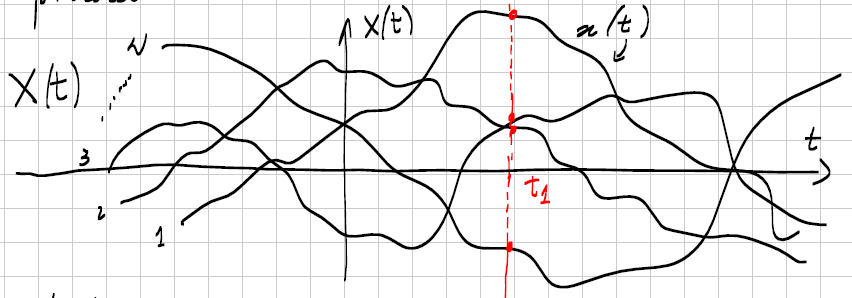
\includegraphics[width=0.9\textwidth]{aleatori-01}
\end{center}

Volendo dare una definizione pi� precisa e matematicamente rigorosa di \emph{processo aleatorio}, � necessario innanzitutto considerare un \emph{esperimento aleatorio} o, meglio, uno \emph{spazio di probabilit�} caratterizzato da uno spazio campione $\Omega=\{\omega_i\}$ (qui per semplicit� discreto), da una classe degli eventi $S$ e dalla legge di probabilit� $\Pr\{\cdot\}$ definita su $S$. Si deve poi individuare un insieme di \emph{funzioni del tempo} $x_i(t)$ (le \emph{funzioni campione}) in numero pari a quello dei risultati dell'esperimento $\omega_i$. Infine, si deve \emph{istituire} \emph{una corrispondenza} che associa a ciascun risultato $\omega_i$ dell'esperimento una delle possibili funzioni campione $x_i(t)$:
%
\begin{equation}\label{eq:processo-aleatorio}
X(\omega_i;t) = x_i(t).
\end{equation}
%
Questa corrispondenza costituisce appunto il \emph{processo aleatorio}, il quale si indica comunemente con $X(t)$ omettendo per semplicit� la dipendenza dal risultato $\omega_i$ dello spazio campione $\Omega$. Tale dipendenza, in ogni caso, va sempre considerata implicita. Quando si effettua una \emph{prova} dell'esperimento (una misura di un elettrocardiogramma), si ha un \emph{risultato} dello spazio campione (un paziente) cui � associata una funzione campione (un elettrocardiogramma), cio� il segnale che effettivamente viene osservato, e che prende il nome di \emph{realizzazione} del processo.%
\footnote{Normalmente, \emph{realizzazione} viene usata come sinonimo di \emph{funzione campione}. In realt�, le funzioni campione sono tutti i \emph{possibili} segnali del processo, mentre la realizzazione � quello tra i possibili segnali che viene effettivamente osservato in una data prova dell'esperimento.}

Fissare nel processo aleatorio $X(\omega_i;t)$ il risultato dell'esperimento, ad esempio $\omega_i$, significa selezionare quella tra le varie funzioni campione che si � \emph{realizzata} in una data prova; non c'� pi� alcuna aleatoriet� e il processo diventa \emph{a posteriori} il segnale \emph{determinato} $X(\omega_i;t)$, cio� la funzione campione $x_i(t)$.

Viceversa, se fissiamo arbitrariamente un certo istante di tempo $\bar{t}$, il valore del processo $X(\omega_i;\bar{t})$ all'istante fissato � un insieme di valori ottenuti ``campionando'' le funzioni campione a quell'istante: in una parola, � una \emph{variabile aleatoria}, in accordo con il concetto elementare che segnale aleatorio � un segnale il cui valore a un dato istante non � esattamente determinabile. (I processi stocastici, d'altro canto, possono esser visti come variabili aleatorie che dipendono anche dal tempo.)


\subsection{Caratterizzazione statistica di un processo aleatorio}

� chiaro a questo punto che, contrariamente al caso di un segnale determinato, non ha senso parlare dell'\emph{andamento} di un processo. D'altronde, l'elencazione esaustiva di tutte le funzioni campione del processo � un procedimento impensabile nella grande maggioranza dei casi. Si pone quindi il problema della \emph{caratterizzazione} delle propriet� di un processo dal punto di vista \emph{statistico}.

Fissato l'istante $t=t_1$, il valore del processo $X(t_1)$ a quell'istante � una variabile aleatoria, il cui comportamento statistico pu� essere descritto mediante la sua \emph{funzione distribuzione di probabilit�}.%
\footnote{La \emph{funzione distribuzione di probabilit�} $F_X(x)$ di una \emph{variabile} aleatoria $X$ � definita come:
\[F_X(x)\triangleq \Pr\{X\leq x\}\]
dove con $\Pr\{\cdot\}$ si � indicata la \emph{legge di probabilit�}, che associa a ogni evento una misura della sua probabilit� di presentazione, e dove $x$ � un valore reale generico ma \emph{fissato} (una sorta di valore di ``sonda'') che identifica l'evento $\{X\leq x\}$ di cui si deve calcolare la probabilit�.}
%
Si definisce perci� la \emph{funzione distribuzione di probabilit� del I ordine del processo} mediante la relazione
%
\begin{align}
F_X(x;t_1) &\triangleq \Pr\{X(t_1)\leq x\}
\end{align}
%
dove la legge di probabilit� $\Pr\{\cdot\}$ � per definizione uguale a sua volta al limite per $n\to\infty$ del rapporto tra il numero di osservazioni per cui $X(t_1)\leq x$ e il numero totale delle osservazioni:
%
\begin{align}
F_X(x;t_1) &\triangleq \lim_{n\to\infty}\frac{n_{X(t_1)\leq x}}{n}.
\end{align}

\begin{figure}
\centering
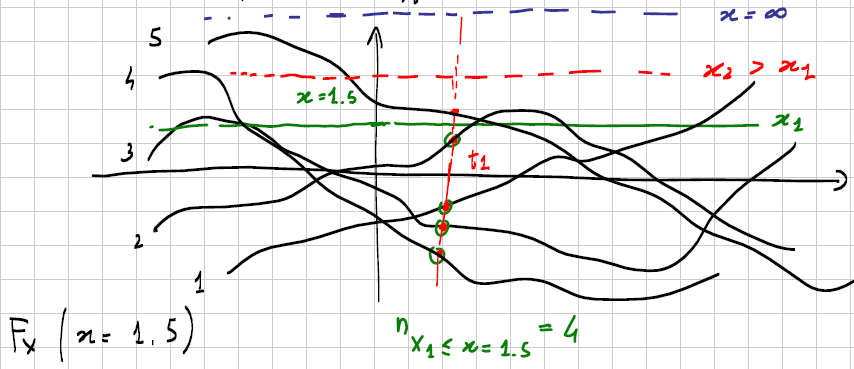
\includegraphics[width=0.9\textwidth]{aleatori-02}
\caption{Funzione distribuzione di probabilit� del primo ordine di un processo aleatorio. Essendo il numero totale degli esperimenti fatti $n=5$, la $F_X(x;t)$ valutata all'istante $t_1$ per $x=1.5$ vale $4/5=0.8$.}
\end{figure}

Da questa formulazione seguono direttamente alcune propriet� della distribuzione di probabilit� $F_X(x;t)$:
%
\begin{enumerate}
\item Il limite per $x\to+\infty$ � unitario:\label{p:limite-unitario}
      \[F_X(+\infty)=1 \quad\text{ o meglio }\quad\lim_{x\to+\infty}F_X(x;t) = 1 \quad\text{per ogni }t.\]
\item Il limite per $x\to-\infty$ � nullo:
      \[F_X(-\infty)=0 \quad\text{ o meglio }\quad\lim_{x\to-\infty}F_X(x;t) = 0 \quad\text{per ogni }t.\]
\item � compresa tra $0$ e $1$:
      \[0\leq F_X(x;t)\leq 1 \quad\text{ per ogni }x,t.\]
\item � una funzione monotona non decrescente, ovvero:
      \[x_2>x_1 \quad\Longrightarrow\quad F_X(x_2;t)\geq F_X(x_1;t).\]
\item La\margincomment{Propriet� riportata in~\citep[pag.~383]{b:luise} ma non citata dal professore.} probabilit� dell'evento $\{x_1<X(t)\leq x_2\}$ pu� essere calcolata mediante la relazione:
      \[\Pr\{x_1< X(t)\leq x_2\} = F_X(x_2;t)-F_X(x_1;t).\]
\end{enumerate}

Una descrizione completa del tutto equivalente (e anche pi� usata in pratica) si basa sulla \emph{funzione densit� di probabilit� del I ordine} del processo:
%
\begin{equation}
f_X(x;t) \triangleq \frac{\partial F_X(x;t)}{\partial x}
\end{equation}
%
da cui si ricava immediatamente la relazione inversa:
%
\[F_X(x;t) = \int_{-\infty}^{x} f_X(\alpha;t)\ud\alpha.\]

La funzione densit� di probabilit� $f_X(x;t)$ gode delle seguenti propriet�:
%
\begin{enumerate}
\item � non negativa, ovvero:
      \[f_X(x;t)\geq 0\]
      poich� la funzione distribuzione di probabilit� � monotona non decrescente.
\item L'integrale su tutto l'asse reale della funzione densit� � unitario:
      \[\int_{-\infty}^{+\infty}f_X(x;t)\ud x = 1\]
      in quanto questo integrale rappresenta la probabilit� dell'evento certo (deriva dalla propriet� \ref{p:limite-unitario} della distribuzione di probabilit�).
\item La probabilit� dell'evento $\{x_1<X(t)\leq x_2\}$ pu� essere calcolata mediante la relazione:
      \[\Pr\{x_1< X(t)\leq x_2\} = F_X(x_2;t)-F_X(x_1;t) = \int_{x_1}^{x_2}f_X(x;t)\ud x.\]
\end{enumerate}

La funzione $f_X(x;t)$ (o equivalentemente la $F_X(x;t)$) non � sufficiente a caratterizzare completamente le propriet� del processo. Consente di caratterizzare variabili aleatorie estratte dal processo purch� considerate \emph{singolarmente}, ma da essa non si pu� ricavare una probabilit� come \annotation[caption={Probabilit� congiunta.}]{ad esempio}{Ma anche avendo la densit� di ordine $n$-esimo, come si fa a calcolare questa probabilit�?}
%
\[\Pr\{X(t_2)\geq X(t_1)\},\]
%
che richiede la considerazione \emph{congiunta} di \emph{due} variabili aleatorie estratte dallo stesso processo in \emph{istanti distinti}. Se c'� un'influenza reciproca tra i valori assunti dalle due variabili, le sole funzioni $F_X(x;t_1)$ e $F_X(x;t_2)$ non bastano, poich� non danno alcuna informazione sul comportamento congiunto delle due variabili aleatorie, ma riguardano \emph{solo} una grandezza senza minimamente tener conto anche dell'altra.

Estraendo dal processo $X(t)$ le due variabili aleatorie $X(t_1)$ e $X(t_2)$, il comportamento statistico di questa coppia di variabili aleatorie � completamente descritto dalla loro \emph{funzione distribuzione di probabilit� del II ordine del processo}:
%
\begin{equation}
F_x(x_1,x_2;t_1,t_2) \triangleq \Pr\{(X(t_1)\leq x_1)\cap(X(t_2)\leq x_2)\}
\end{equation}
%
(la quale, come vedremo, determina anche le propriet� statistiche \emph{marginali}, cio� relative a una sola variabile della coppia). Essa misura la probabilit� che si verifichino congiuntamente i due eventi $X(t_1)\leq x_1$ e $X(t_2)\leq x_2$.

La funzione distribuzione di probabilit� del II ordine gode delle seguenti propriet�:
\begin{enumerate}
\item La funzione $F_{X}(x_1,x_2;t_1,t_2)$, comunque si scelga il valore $x_1$ � monotona non decrescente al variare di $x_2$; analogamente, comunque si scelga il valore $x_2$, � monotona non decrescente al variare di $x_1$.
\item Soddisfa le uguaglianze:
      \[F_{X}(-\infty, x_2) = 0 \quad\text{ e }\quad F_{X}(x_1, -\infty) = 0.\]
\item Il limite per $x_1,x_2\to+\infty$ � unitario:
      \[F_X(+\infty,+\infty) = 1\]
\item � compresa tra $0$ e $1$:
      \[0 \leq F_X(x_1,x_2) \leq 1.\]
\item Le funzioni distribuzione \emph{marginali} delle variabili aleatorie $X(t_1)$ e $X(t_2)$ si ricavano dalla congiunta come segue:
\begin{align}\label{eq:regole-marginali}
\begin{split}
F_X(x_1) &= F_{X}(x_1, +\infty)\\
F_X(x_2) &= F_{X}(+\infty, x_2).
\end{split}
\end{align}
\end{enumerate}

La \emph{funzione densit� di probabilit� del II ordine} di un processo � espressa dalla:
%
\begin{equation}
f_X(x_1,x_2;t_1,t_2) \triangleq \frac{\partial^2F_X(x_1,x_2;t_1,t_2)}{\partial x_1\partial x_2}
\end{equation}
%
da cui la relazione inversa:
%
\begin{equation}
F_X(x_1,x_2;t_1,t_2) = \int_{-\infty}^{x_1}\int_{-\infty}^{x_2} f_X(\alpha_1,\alpha_2;t_1,t_2)\ud\alpha_1\ud\alpha_2
\end{equation}
%
e gode di propriet� simili a quelle gi� viste per la densit� di probabilit� del I ordine, ad esempio:
%
\begin{itemize}
\item � non negativa:
      \[f_X(x_1,x_2;t_1,t_2) \geq 0.\]
\item L'integrale � unitario:
      \[\int_{-\infty}^{+\infty}\int_{-\infty}^{+\infty} f_X(\alpha_1,\alpha_2;t_1,t_2)\ud\alpha_1\ud\alpha_2 = 1.\]
\end{itemize}

Come � chiaro, il ragionamento che ha portato a estendere la descrizione dal primo al secondo ordine pu� essere iterato a piacere. La conclusione � che la descrizione statistica di un processo � \emph{completa} solo quando si � in grado di caratterizzare il comportamento statistico \emph{congiunto} di un numero $n$ arbitrario di variabili aleatorie $X(t_1)$, $X(t_2)$, \dots, $X(t_n)$ estratte da $X(t)$ a $n$ istanti diversi, comunque grande sia il numero intero $n$ e comunque si scelga la $n$-upla di istanti $(t_1, t_2, \dots, t_n)$. Ci� richiede, quindi, la conoscenza della \emph{funzione distribuzione di probabilit� dell'\/$n$-esimo ordine}:
%
\begin{equation}
F_X(\underline{x};\underline{t}) \triangleq \Pr\{(X(t_1)\leq x_1)\cap\dots\cap(X(t_n)\leq x_n)\}
\end{equation}
%
o, equivalentemente, la \emph{funzione densit� di probabilit� di ordine $n$}:
%
\begin{equation}
f_X(\underline{x};\underline{t}) \triangleq \frac{\partial^nF_X(\underline{x};\underline{t})}{\partial x_1\dots\partial x_n},
\end{equation}
%
avendo definito i vettori $\underline{x}=(x_1,\dots,x_n)$ e $\underline{t}=(t_1,\dots,t_n)$.


\subsection{Classi di variabili aleatorie}

Classifichiamo ora le variabili aleatorie in alcune classi, a seconda del comportamento che presentano.
%
\begin{itemize}
\item\emph{Variabili aleatorie uniformemente distribuite.} Una variabile aleatoria $X$ si dice \emph{uniforme} sull'intervallo $[a, b]$, e si scrive $X\in\mathcal{U}[a,b]$, se la sua densit� di probabilit� $f_X(x)$ � costante in tale intervallo e si annulla al di fuori di esso. Poich� l'integrale deve essere unitario, il valore della funzione su $[a,b]$ deve essere evidentemente pari a $1/(b-a)$:
\[f_X(x) = \begin{cases}\frac{1}{b-a}& \text{se }x\in[a,b]\\0&\text{altrove.}\end{cases}\]
Ogni evento del tipo $\{X \leq x\}$ ha sempre la medesima probabilit� di verificarsi indipendentemente dalla posizione di $x$, purch� $x\in[a,b]$.
%
\begin{figure}[t]
\centering
\subfloat{\framebox{\begin{pspicture*}(-1.5,-0.8)(4.3,2.2)
  \psaxes[linewidth=0.4pt,labels=none,ticks=none]{->}(0,0)(-1.3,-0.6)(4.1,2)
  \psline[linewidth=1pt](-0.3,0)(0.5,0)
  \psline[linewidth=0.5pt](0.5,0)(0.5,1)
  \psline[linewidth=1pt](0.5,1)(2.4,1)
  \psline[linewidth=0.5pt](2.4,0)(2.4,1)
  \psline[linewidth=1pt](2.4,0)(3,0)
  \psline[linewidth=1pt,linestyle=dashed,dash=2pt 2pt](-0.9,0)(-0.3,0)
  \psline[linewidth=1pt,linestyle=dashed,dash=2pt 2pt](3,0)(3.8,0)
  \uput[l](0,1.8){$f_X(x)$}
  \uput[d](4,0){$x$}
  \uput[d](0.5,-0.1){$a$}
  \uput[d](2.4,0){$b$}
  \uput[l](0,1){$\frac{1}{b-a}$}
  \psline[linewidth=0.5pt](-0.05,1)(0.05,1)
\end{pspicture*}}} \quad
\subfloat{\framebox{\begin{pspicture*}(-1.5,-0.8)(4.3,2.2)
  \psaxes[linewidth=0.4pt,labels=none,ticks=none]{->}(0,0)(-1.3,-0.6)(4.1,2)
  \psline[linewidth=1pt](-0.3,0)(0.5,0)
  \psline[linewidth=1pt](0.5,0)(2.4,1)
  \psline[linewidth=1pt](2.4,1)(3,1)
  \psline[linewidth=1pt,linestyle=dashed,dash=2pt 2pt](-0.9,0)(-0.3,0)
  \psline[linewidth=1pt,linestyle=dashed,dash=2pt 2pt](3,1)(3.8,1)
  \uput[l](0,1.8){$F_X(x)$}
  \uput[d](4,0){$x$}
  \uput[d](0.5,-0.1){$a$}
  \uput[d](2.4,0){$b$}
  \psline[linewidth=0.5pt](2.4,-0.05)(2.4,0.05)
  \uput[l](0,1){$\scriptstyle{1}$}
  \psline[linewidth=0.5pt](-0.05,1)(0.05,1)
\end{pspicture*}}}
\caption{Densit� e distribuzione di probabilit� di una variabile aleatoria uniforme.}
\end{figure}

\item\emph{Variabile esponenziale unilatera.} Una variabile aleatoria $X$ � esponenziale unilatera se la sua densit� di probabilit� $f_X(x)$ � espressa dalla relazione
\[f_X(x) = \frac{1}{\eta}\e^{-\frac{x}{\eta}}\u(x)\]
ove $\eta$ � un parametro reale positivo. La funzione distribuzione $F_X(x)$ � allora:
\begin{align*}
F_X(x) &= \int_{-\infty}^{x}\frac{1}{\eta}\e^{-\frac{\alpha}{\eta}}\u(\alpha)\ud\alpha\\
       &= \int_0^x \frac{1}{\eta}\e^{-\frac{\alpha}{\eta}}\ud\alpha\\
       &= \left.-\e^{-\frac{\alpha}{\eta}}\right|_0^x = (1-\e^{-\frac{x}{\eta}})\u(x).
\end{align*}
Le variabili aleatorie appartenenti a questa classe si indicano con $\mathcal{E}[\eta]$.
%
\begin{figure}[!b]
\centering
\subfloat{\framebox{\begin{pspicture*}(-1.5,-0.7)(4.3,2.1)
  \psaxes[linewidth=0.5pt,labels=none,ticks=none]{->}(0,0)(-1.3,-0.1)(4,1.9)
  \uput[d](3.9,0){$x$}
  \uput[r](0,1.7){$f_X(x)$}
  \uput[l](0,1.31){$\frac{1}{\eta}$}
  \psline[linewidth=0.5pt](-0.05,1.31)(0.05,1.31)
  \infixtoRPN{1.31*2.718^(-x/1.1)}
  \psline[linewidth=1pt,linestyle=dashed,dash=2pt 2pt](-0.9,0)(-0.3,0)
  \psline[linewidth=1pt](-0.3,0)(0,0)
  \psplot[linewidth=1pt,plotstyle=curve,plotpoints=200]{0}{3.2}{\RPN}
  \psplot[linewidth=1pt,plotstyle=curve,plotpoints=50,linestyle=dashed,dash=2pt 2pt]{3.2}{3.6}{\RPN}
\end{pspicture*}}} \quad
\subfloat{\framebox{\begin{pspicture*}(-1.5,-0.7)(4.3,2.1)
  \psaxes[linewidth=0.5pt,labels=none,ticks=none]{->}(0,0)(-1.3,-0.1)(4,1.9)
  \uput[d](3.9,0){$x$}
  \uput[r](0,1.7){$F_X(x)$}
  \uput[l](0,1){$1$}
  \psline[linewidth=1pt,linestyle=dashed,dash=2pt 2pt](-0.9,0)(-0.3,0)
  \psline[linewidth=1pt](-0.3,0)(0,0)
  \psline[linewidth=0.5pt,linestyle=dashed,dash=1pt 1pt](-0.05,1)(3.6,1)
  \infixtoRPN{1-2.71^(-x/0.9)}
  \psplot[linewidth=1pt,plotstyle=curve,plotpoints=200]{0}{3.2}{\RPN}
  \psplot[linewidth=1pt,plotstyle=curve,plotpoints=50,linestyle=dashed,dash=2pt 2pt]{3.2}{3.6}{\RPN}
\end{pspicture*}}}
\caption{Densit� e distribuzione di probabilit� di una variabile aleatoria esponenziale unilatera.}
\end{figure}

\item\emph{Variabile esponenziale bilatera.} Una variabile aleatoria $X$ � esponenziale unilatera se la sua densit� di probabilit� $f_X(x)$ � espressa dalla relazione
\[f_X(x) = \frac{1}{2\eta}\e^{-\frac{\abs{x}}{\eta}}\u(x).\]
Le variabili aleatorie appartenenti a questa classe si indicano con $\mathcal{E}_2[\eta]$.
%
\begin{figure}[t]
\centering
\framebox{\begin{pspicture*}(-4.7,-0.7)(5.3,2.1)
  \psaxes[linewidth=0.5pt,labels=none,ticks=none]{->}(0,0)(-4.5,-0.1)(5,1.9)
  \uput[d](4.9,0){$x$}
  \uput[r](0,1.7){$f_X(x)$}
  \uput[l](-0.2,1.2){$\frac{1}{2\eta}$}
  \infixtoRPN{1.2*2.718^(-abs(x)/1.1)}
  \psplot[linewidth=1pt,plotstyle=curve,plotpoints=50,linestyle=dashed,dash=2pt 2pt]{-4.3}{-3.3}{\RPN}
  \psplot[linewidth=1pt,plotstyle=curve,plotpoints=200]{-3.3}{3.6}{\RPN}
  \psplot[linewidth=1pt,plotstyle=curve,plotpoints=50,linestyle=dashed,dash=2pt 2pt]{3.6}{4.6}{\RPN}
\end{pspicture*}}
\caption{Funzione densit� di probabilit� di una variabile aleatoria esponenziale bilatera.}
\end{figure}

\item\emph{Variabili aleatorie gaussiane o normali.} 
Si denotano con la scrittura $\mathcal{N}(\eta,\sigma^2)$ e sono caratterizzate da una densit� di probabilit� a forma di ``campana di Gauss'':
\[f_X(x;t) = \frac{1}{\sqrt{2\pi}\sigma}\e^{-\frac{(x-\eta)^2}{2\sigma^2}}.\]
%
\begin{figure}[t]
\centering
\framebox{\begin{pspicture*}(-4.7,-0.7)(5.3,2.1)
  \psaxes[linewidth=0.5pt,labels=none,ticks=none]{->}(0,0)(-4.5,-0.1)(5,1.9)
  \uput[d](4.9,0){$x$}
  \uput[r](0,1.7){$f_X(x)$}
  \uput[l](-0.2,1.2){$\frac{1}{\sqrt{2\pi}\sigma}$}
  \psline[linewidth=0.5pt](-0.05,1.2)(0.05,1.2)
  \infixtoRPN{1.2*2.718^(-((x-1)^2)/1.1)}
  \psplot[linewidth=1pt,plotstyle=curve,plotpoints=50,linestyle=dashed,dash=2pt 2pt]{-4.3}{-3.3}{\RPN}
  \psplot[linewidth=1pt,plotstyle=curve,plotpoints=200]{-3.3}{3.6}{\RPN}
  \psplot[linewidth=1pt,plotstyle=curve,plotpoints=50,linestyle=dashed,dash=2pt 2pt]{3.6}{4.6}{\RPN}
  \psline[linewidth=0.5pt](1,-0.05)(1,0.05)
  \uput[d](1,0){$\eta$}
\end{pspicture*}}
\caption{Funzione densit� di probabilit� di una variabile aleatoria gaussiana.}
\end{figure}

\end{itemize}



\section{Indici statistici del I e II ordine di un processo aleatorio}

� abbastanza chiaro che, assegnato un processo $X(t)$, � impresa disperata pervenire alla sua conoscenza statistica completa. In alcuni casi � sufficiente in realt� conoscere la distribuzione (o densit�) di probabilit� del primo ordine, raramente si cerca di misurare o calcolare quella del secondo. Molto pi� spesso ci si accontenta di \emph{parametri statistici semplificati}, discussi in questo paragrafo.

\subsection{Indici del I ordine: valor medio, potenza, varianza}

Una grandezza particolarmente significativa nella descrizione statistica semplificata di un processo aleatorio $X(t)$ � la sua funzione \emph{valor medio statistico} $\eta_X(t)$. Per definizione, il valore di questa funzione a un istante $t$ � il valor medio della variabile aleatoria $X(t)$, estratta dal processo all'istante stesso:%
\footnote{Quando si ha a che fare con un problema di \emph{trasformazione} di una variabile aleatoria $Y = g(X)$ (o anche di un processo aleatorio), si introduce il cosiddetto \emph{operatore valor medio}:
%
\[\E\{g(X)\}\triangleq \int_{-\infty}^{+\infty} g(x)f_X(x)\ud x\]
%
che pu� esser visto come una \emph{somma} dei valori $g(x)$ \emph{pesata} dalla densit� di probabilit� di $X$. La lettera ``E'' � l'iniziale della parola inglese \emph{expectation}, traducibile in italiano con ``aspettativa''. Si noti che, essendo un integrale, gode della propriet� di linearit�.}
%
\begin{equation}
\eta_X(t) \triangleq \E\{X(t)\} = \int_{-\infty}^{+\infty} xf_X(x;t)\ud x.
\end{equation}
%
Pu� esser vista come l'integrale di tutti i valori della $x$ che il processo pu� assumere pesato ciascuno con la relativa probabilit� di presentazione: $\eta_X(t)$ rappresenta in certo senso un valore ``baricentrico'' attorno al quale si distribuiscono i valori della variabile aleatoria $X(t)$ stessa (perci� � un indice di \emph{posizione}).

La funzione valor medio � una \emph{statistica del primo ordine} di $X(t)$ poich� il suo calcolo prevede la considerazione di una sola variabile aleatoria estratta dal processo, e quindi \emph{richiede la conoscenza della sola densit� di probabilit� del primo ordine}.

Un'altra grandezza statistica del primo ordine utile per caratterizzare statisticamente il processo $X(t)$ � la funzione \emph{potenza media statistica istantanea $P_X(t)$} (detta brevemente, \emph{potenza media}):
%
\begin{equation}\label{eq:potenza-processo}
P_X(t) \triangleq \E\{\abs{X(t)}^2\} = \int_{-\infty}^{+\infty} \abs{x}^2f_X(x;t)\ud x.
\end{equation}

Per i segnali aleatori si definisce anche la \emph{funzione varianza} del processo:
%
\begin{equation}\label{eq:varianza-processo}
\sigma^2_X(t) \triangleq \E\{\abs{X(t)-\eta_X(t)}^2\} = \int_{-\infty}^{+\infty}\abs{x-\eta_X(t)}^2f_X(x;t)\ud x
\end{equation}
%
cio� la varianza della variabile aleatoria ottenuta fissando l'istante $t$. Pu� anche essere espressa come la potenza media istantanea del \emph{processo di scarto}, definito come il processo di partenza a meno del valor medio:
%
\[L_X(t) = X(t)- \eta_X(t).\]

Nelle~\eqref{eq:potenza-processo}%
\margincomment{Questa relazione vale in generale anche per segnali complessi, scrivendo come ovvio: $\sigma_X^2(t) = P_X(t)-\abs{\eta_X(t)}^2$.}
e~\eqref{eq:varianza-processo} spesso scompare il modulo, avendo a che fare con segnali reali. Proprio considerando segnali reali, sviluppando la~\eqref{eq:varianza-processo} si ricava facilmente la relazione tra potenza media e varianza:
%
\begin{equation}\label{eq:relazione-potenza-media-varianza}
\sigma_X^2(t) = P_X(t)-\eta_X^2(t).
\end{equation}
%
Infatti, tenendo conto che la $\eta_X(t)$ � una funzione deterministica, si ha:
%
\begin{align*}
\sigma^2_X(t) &= \E\{\bigl(X(t)-\eta_X(t)\bigr)^2\}\\
   &= \E\{X^2(t)\} - 2\E\{\eta_X(t)\cdot X(t)\} + \E\{\eta_X^2(t)\}\\
   &= P_X(t) - 2\eta_X(t)\E\{X(t)\} + \eta_X^2(t)\\
   &= P_X(t) - \eta^2_X(t).
\end{align*}
%
Si pu� anche dire, in certi termini, che la varianza equivale alla differenza tra l'aspettazione del quadrato e il quadrato dell'aspettazione.

La radice quadrata $\sigma_X(t)\geq 0$ della varianza � la \emph{deviazione standard}, che � un \emph{indice di dispersione}, poich� rappresenta di quanto ci si discosta dal valore medio.  A maggiore varianza corrispondono valori molto dispersi attorno al valor medio, e viceversa. Al limite, una variabile aleatoria con varianza nulla ha valori \emph{per niente} dispersi attorno al valor medio e la sua densit� di probabilit� diventa ``infinitamente appuntita'' (una delta di Dirac) attorno a $\eta_X$: in pratica la variabile aleatoria ``collassa'' in un valore \emph{certo}.

\begin{figure}[t]
\centering
\framebox{\begin{pspicture*}(-4.7,-0.9)(5.3,2.1)
  \psaxes[linewidth=0.5pt,labels=none,ticks=none]{->}(0,0)(-4.5,-0.1)(5,1.9)
  \uput[d](4.9,0){$x$}
  \uput[l](2.7,1.5){$\scriptstyle{f_X(x;t_1)}$}
  \uput[r](-2.6,1){$\scriptstyle{f_X(x;t_2)}$}
  \psline[linewidth=0.5pt]{->}(-1.9,0.7)(-1.3,0.4)
  \psline[linewidth=0.5pt]{->}(1.9,1.2)(1.3,1)
  \psplot[linewidth=1pt,plotstyle=curve,plotpoints=200]% 10*\e^(-abs(x/12)^2)
         {-4.3}{4.6}{0.8 2.718281828459045235 x 0.5 sub 1.5 div abs 2 exp neg exp mul}
  \psplot[linewidth=1pt,plotstyle=curve,plotpoints=200]% 10*\e^(-abs(x/12)^2)
         {-4.3}{4.6}{1.4 2.718281828459045235 x 0.5 sub 0.8 div abs 2 exp neg exp mul}
  \psline[linewidth=0.5pt](0.5,-0.05)(0.5,0.05)
  \psline[linewidth=0.5pt,linestyle=dashed,dash=1pt 1pt](0.5,0.05)(0.5,1.4)
  \uput[d](0.5,0){$\scriptscriptstyle{\eta_X(t_1)}$}
  \uput[d](0.5,-0.28){$\scriptscriptstyle{\eta_X(t_2)}$}
\end{pspicture*}}
\caption{La varianza fornisce un indice di dispersione, che rappresenta quanto poco i valori sono concentrati attorno al valor medio.}
\label{fig:dispersione-attorno-al-valor-medio}
\end{figure}
%
Si consideri il grafico nella figura~\ref{fig:dispersione-attorno-al-valor-medio}. Si noti, innanzitutto, che si � supposto che il valor medio $\eta_X(t_2)$ della variabile aleatoria $X(t_2)$ coincida con $\eta_X(t_1)$. Si ha una situazione in cui $\sigma_X(t_2)>\sigma_X(t_1)$, ossia la densit� di probabilit� $f_X(x;t_2)$ ha una dispersione maggiore attorno al suo valor medio rispetto alla dispersione della $f_X(x;t_1)$ attorno a $\eta_X(t_1)$.


\subsection{Indici del II ordine: autocorrelazione e autocovarianza}

Introduciamo adesso due parametri statistici del \emph{secondo ordine} di fondamentale importanza per lo studio dei segnali aleatori.

Fissiamo due istanti di tempo arbitrari $t_1$ e $t_2$ sul nostro processo, ottenendo le due variabili aleatorie $X(t_1)$ e $X(t_2)$. La \emph{funzione di autocorrelazione} del processo si calcola come correlazione%
\footnote{La \emph{correlazione} tra due \emph{variabili} aleatorie $X$ e $Y$ si calcola come:
\[r_{XY} \triangleq \E\{XY^*\} = \int_{-\infty}^{+\infty}\int_{-\infty}^{+\infty} xyf_{XY}(x,y)\ud x\ud y.\]}
tra queste due variabili aleatorie:
%
\[R_X(t_1,t_2) \triangleq \E\{X(t_1)X^*(t_2)\} = \int_{-\infty}^{+\infty}\int_{-\infty}^{+\infty}x_1x_2f_X(x_1,x_2;t_1,t_2)\ud x_1 \ud x_2.\]
%
Naturalmente, il valore di questa correlazione risulter� \emph{funzione dei due istanti $t_1$ e $t_2$} ai quali le variabili sono state estratte, e potr� essere calcolata solo conoscendo la funzione densit� di probabilit� \emph{del secondo ordine} del processo. Inoltre, si chiama funzione di \emph{auto}correlazione perch� le due variabili aleatorie di cui si calcola la correlazione sono estratte dallo \emph{stesso} processo aleatorio.

\begin{definizione}
Due variabili aleatorie si dicono \emph{ortogonali} quando la loro correlazione � nulla.
\end{definizione}

Se invece tra le due variabili aleatorie $X(t_1)$ e $X(t_2)$ calcoliamo la covarianza%
\footnote{La \emph{covarianza} tra due \emph{variabili} aleatorie � definita come:
\[c_{XY} \triangleq \E\{(X-\eta_X)(Y-\eta_Y)\} = \int_{-\infty}^{+\infty}\int_{-\infty}^{+\infty} (x-\eta_X)(y-\eta_Y)f_{XY}(x,y)\ud x\ud y.\]}
otteniamo la \emph{funzione di autocovarianza} di $X(t)$:
%
\begin{align*}
C_X(t_1,t_2) &\triangleq \E\big\{\big(X(t_1)-\eta_X(t_1)\big)\big(X(t_2)-\eta_X(t_2)\big)^*\big\}\\
    &= \int_{-\infty}^{+\infty}\int_{-\infty}^{+\infty}
       \big(x_1-\eta_X(t_1)\big)\big(x_2-\eta_X(t_2)\big) f_X(x_1,x_2;t_1,t_2)\ud x_1\ud x_2
\end{align*}
%
che equivale alla funzione di autocorrelazione del processo di scarto:
%
\[C_X(t_1,t_2) = R_{L_X}(t_1,t_2) = \E\{L_X(t_1)L_X^*(t_2)\}.\]

La%
\margincomment{Da~\citep[pag.~412]{b:luise}.}
covarianza � un parametro statistico molto importante che tende ad accertare se tra le due variabili $X(t_1)$ e $X(t_2)$ esiste una relazione di dipendenza di tipo \emph{lineare}, e che comunque misura la tendenza di variazione congiunta (perci� \emph{co}-varianza) delle due. Se la covarianza � grande e positiva, le due variabili aleatorie $X(t_1)$ e $X(t_2)$ tendono a discostarsi dal rispettivo valor medio nella stessa direzione, cio� le due quantit� $(X(t_1)-\eta_X(t_1))$ e $(X(t_2)-\eta_X(t_2))$ tendono ad avere lo stesso segno.

\begin{definizione}
Due variabili aleatorie si dicono \emph{incorrelate} quando la loro covarianza � nulla.
\end{definizione}

� facile verificare che se due variabili aleatorie $X(t_1)$ e $X(t_2)$ sono ortogonali e inoltre $\eta_X(t)=0$, allora esse sono anche incorrelate.

Le%
\margincomment{Il professore preferisce scriverle quasi sempre in questa forma.}
funzioni di autocorrelazione e autocovarianza possono essere espresse anche in una forma leggermente diversa. Ponendo $t_2=t$ e $t_1=t+\tau$, sono:
%
\begin{align}
R_X(t+\tau,t) &= \E\{X(t+\tau)X^*(t)\}\\
C_X(t+\tau,t) &= \E\big\{\big(X(t+\tau)-\eta_X(t+\tau)\big)\big(X(t)-\eta_X(t)\big)^*\big\}.
\end{align}

Da queste definizioni si ricava immediatamente la relazione:
%
\begin{equation}\label{eq:relazione-autocovarianza-autocorrelazione}
C_X(t+\tau,t) = R_X(t+\tau,t) - \eta_X(t+\tau)\eta_X(t).
\end{equation}
%
Infatti, se consideriamo segnali reali:
%
\begin{align*}
C_X(t+\tau,t) &= \E\big\{\big(X(t+\tau)-\eta_X(t+\tau)\big)\big(X(t)-\eta_X(t)\big)^*\big\}\\
    &= \E\{X(t+\tau)X(t)-X(t+\tau)\eta_X(t)\\
    &\quad -\eta_X(t+\tau)X(t)+\eta_X(t+\tau)\eta_X(t)\}\\
    &= \E\{X(t+\tau)X(t)\}-\eta_X(t)\E\{X(t+\tau)\}\\
    &\quad -\eta_X(t+\tau)\E\{X(t)\}+\eta_X(t+\tau)\eta_X(t)\\
    &= R_X(t+\tau,t) - \eta_X(t)\eta_X(t+\tau)
\end{align*}

Se fissiamo gli istanti $t_1=t_2=t$ (o equivalentemente $\tau=0$), la funzione di autocorrelazione fornisce la potenza media del processo:
%
\[R_X(t,t) = \left.R_X(\tau)\right|_{\tau=0} = \E\{X(t)X^*(t)\} = \E\{X^2(t)\} = P_X(t)\]
%
mentre la funzione di covarianza restituisce la varianza:
%
\[C_X(t,t) = \left.C_X(\tau)\right|_{\tau=0} = \E\{(X(t)-\eta_X(t))^2\} = \sigma^2_X(t).\]
%
cosicch� la relazione~\eqref{eq:relazione-autocovarianza-autocorrelazione} diventa uguale alla~\eqref{eq:relazione-potenza-media-varianza}.



\section{Processi aleatori stazionari}

\subsection{Stazionariet� in senso stretto}

Come gi� visto nei precedenti paragrafi, gli indici statistici di un processo, ad esempio la funzione valor medio o la funzione di autocorrelazione e, a maggior ragione, le funzioni densit� di probabilit�, dipendono in generale dalla scelta degli $n$ istanti di tempo $t_1,\dots,t_n$ in corrispondenza dei quali viene valutato il processo. Se \emph{spostiamo rigidamente} tutti gli istanti temporali, cio� consideriamo la nuova $n$-upla di istanti $t_1+\Delta t,\dots,t_n+\Delta t$, con $\Delta t$ arbitrario, in generale, otteniamo un diverso valore della funzione densit� di probabilit� di ordine $n$. Se, viceversa, il valore della funzione densit� resta invariato \emph{qualunque sia $\Delta t$ e per ogni ordine $n$}, allora il processo si dice \acf{SSS}:
%
\begin{align}\label{eq:stazionarieta-in-senso-stretto-1}
\begin{split}
& f_X(x_1,x_2,\dots,x_n; t_1+\Delta t,t_2+\Delta t,\dots,t_n+\Delta t)\\
&\quad = f_X(x_1,x_2,\dots,x_n; t_1,t_2,\dots,t_n) \quad\text{ per ogni }n, \Delta t.
\end{split}
\end{align}
%
La stazionariet� in senso stretto richiede dunque che le funzioni densit� di probabilit� del processo di qualunque ordine siano \emph{invarianti} rispetto a una traslazione rigida degli istanti temporali, e ci� significa che i processi $X(t)$ e $X(t + \Delta t)$ \emph{hanno le stesse statistiche} e quindi sono \emph{equivalenti} dal punto di vista statistico. Ma questo non significa che $X(t+\Delta t)$ sia \emph{uguale} a $X(t)$; infatti, le funzioni campione di $X(t+\Delta t)$ sono ottenute da quelle di $X(t)$ per traslazione temporale, e quindi i due processi sono differenti, bench� indistinguibili con misure statistiche.

Discutiamo ora le conseguenze di questa definizione. Se consideriamo la densit� del primo ordine del processo, la definizione~\eqref{eq:stazionarieta-in-senso-stretto-1} ci dice che deve valere l'uguaglianza
%
\[f_X(x;t) = f_X(x;t+\Delta t), \quad \text{ per ogni } \Delta t.\]
%
Poich� $\Delta t$ � arbitrario, se ne conclude che la densit� di probabilit� del primo ordine $f_X(x;t)$ \emph{non} dipende dal tempo:
%
\begin{equation}\label{eq:stazionarieta-primo-ordine}
f_X(x;t) \equiv f_X(x).
\end{equation}
%
In tal caso il processo � detto \emph{stazionario del I ordine}, e tutte le grandezze statistiche del primo ordine del processo sono a loro volta indipendenti dal tempo:
%
\[\eta_X(t) \equiv \eta_X,\quad P_X(t)\equiv P_X,\quad \sigma_X^2(t)\equiv \sigma_X^2.\]

Consideriamo ora le implicazioni della stazionariet� sulle statistiche del \emph{secondo} ordine. Immaginiamo, allora, di osservare il processo aleatorio $X(t)$ a due istanti arbitrari $t_1$ e $t_2$, estraendo da esso le variabili aleatorie $X(t_1)$ e $X(t_2)$: il comportamento statistico congiunto di tali variabili � descritto dalla funzione $f_X(x_1,x_2;t_1,t_2)$. Se consideriamo, poi, la coppia di variabili aleatorie $X(t_1+\Delta t)$ e $X(t_2+\Delta t)$ estratte agli istanti $t_1+\Delta t$ e $t_2+\Delta t$, deve essere
%
\[f_X(x_1,x_2;t_1,t_2) = f_X(x_1,x_2, t_1+\Delta t,t_2+\Delta t).\]
%
Considerando che anche in questo caso $\Delta t$ � arbitrario, � chiaro che la funzione $f_X(x_1,x_2;t_1,t_2)$ non pu� dipendere da $t_1$ e $t_2$ \emph{separatamente}, ma deve dipendere soltanto dalla \emph{differenza} $t_1-t_2=\tau$ tra gli istanti temporali, che resta appunto invariata in una traslazione rigida dei tempi. La condizione per la \emph{stazionariet� del II ordine} pu� cio� esser scritta come:
%
\begin{equation}\label{eq:stazionarieta-secondo-ordine}
f_X(x_1,x_2;t+\tau,t) \equiv f_X(x_1,x_2;\tau).
\end{equation}
%
Tutte le statistiche del \emph{secondo ordine}, e in particolare la funzione di autocorrelazione e la funzione di autocovarianza, godono evidentemente di questa stessa propriet�:
%
\[R_X(t+\tau,t) \equiv R_x(\tau),\quad C_X(t+\tau,t) \equiv C_X(\tau).\]

Generalizzando, � chiaro che la densit� di probabilit� (e tutte le statistiche) di ordine $n$ di un processo \ac{SSS} dipendono soltanto dalle $(n-1)$ differenze (distanze) tra gli $n$ istanti. La relazione~\eqref{eq:stazionarieta-in-senso-stretto-1} pu� esser perci� riscritta proprio esplicitando le differenze tra gli istanti temporali:
%
\begin{align}\label{eq:stazionarieta-in-senso-stretto-2}
\begin{split}
& f_X(x_1,x_2,\dots,x_n; t,t+\tau_1,\dots,t+\tau_{n-1})\\
&\quad = f_X(x_1,x_2,\dots,x_n; \tau_1,\tau_2,\dots,\tau_{n-1}) \quad\text{ per ogni }n.
\end{split}
\end{align}

Attraverso le ``regole marginali'' (vedi le relazioni~\eqref{eq:regole-marginali} a pag.~\pageref{eq:regole-marginali}) non � difficile verificare che se un processo � stazionario di ordine $n$, allora � stazionario anche di ordine $k\leq n$, mentre se non � stazionario di ordine $k$, allora non sar� stazionario neanche per ogni $m\geq k$.


\subsection{Stazionariet� in senso lato}

La verifica della stazionariet� in senso stretto di un processo �, in generale, estremamente difficoltosa (salvo casi particolari come i \emph{processi gaussiani}, che studieremo nel paragrafo~\ref{sec:processi-gaussiani} a pag.~\pageref{sec:processi-gaussiani}). Di solito nelle applicazioni si considera una definizione di stazionariet� molto meno restrittiva e pi� facile da verificare della precedente: la \emph{stazionariet� in senso lato}.

Un processo aleatorio $X(t)$ � \acf{SSL} se � stazionario in valor medio (ossia $\eta_X(t)$ � \emph{costante}) e se � stazionario in autocorrelazione (ovvero $R_X(t_1,t_2)$ non dipende separatamente dai due istanti ma solo dalla differenza $\tau$):
%
\begin{equation}\label{eq:stazionarieta-in-senso-lato}
\begin{cases}\eta_X(t) = \eta_X\\
R_X(t+\tau,t) = R_X(\tau).\end{cases}
\end{equation}
%
La definizione di stazionariet� in senso lato coinvolge solo due \emph{particolari} statistiche semplificate, una del primo e l'altra del secondo ordine, e \emph{non} richiede alcuna propriet� di invarianza delle densit� di probabilit�. Infatti, un processo stazionario in senso stretto � anche stazionario in senso lato, mentre la stazionariet� in senso lato non implica quella in senso stretto.

Inoltre, se un processo � stazionario del I ordine � anche stazionario in valor medio e analogamente se � stazionario del II ordine � anche stazionario in autocorrelazione, mentre non valgono le implicazioni inverse. Ancora, data la stazionariet� in autocorrelazione, nulla si pu� sapere sulla stazionariet� in valor medio, e viceversa (d'altronde se cos� non fosse le due condizioni~\eqref{eq:stazionarieta-in-senso-lato} si ridurrebbero a una sola).

La stazionariet� in senso lato implica la stazionariet� in autocovarianza:
%
\begin{align*}
C_X(t+\tau,t) &= R_X(t+\tau,t)-\eta_X(t+\tau)\eta_X(\tau)\\
              &= R_X(\tau)-\eta_X^2 = C_X(\tau).
\end{align*}


\subsection{Propriet� della funzione di autocorrelazione di un processo stazionario in senso lato}
\label{sec:proprieta-autocorrelazione-di-processi-ssl}

Per quanto gi� detto, se il processo $X(t)$ � stazionario almeno in senso lato, la funzione di autocorrelazione dipende soltanto dalla \emph{differenza} $\tau$ tra i due istanti:
%
\[R_X(t+\tau,t) = R_X(\tau).\]

La funzione di autocorrelazione $R_X(\tau)$ gode di alcune propriet� fondamentali, non specifiche, in realt�, dei processi, ma comuni alle funzioni di autocorrelazione dei segnali determinati e aleatori. Vediamo, ora, queste propriet� per una processo \ac{SSL}.
%
\begin{enumerate}
\item La funzione di autocorrelazione $R_X(\tau)$ � pari:
      \[R_X(\tau) = R_X(-\tau).\]
      Per dimostrare questa relazione, basta osservare che, per la stazionariet� del processo, la correlazione tra le variabili aleatorie $X(t+\tau)$ e $X(t)$ assume il medesimo valore della correlazione tra le variabili $X(t)$ e $X(t-\tau)$ ottenute per traslazione rigida della quantit� $-\tau$:
      \[R_X(\tau) = \E\{X(t+\tau)X(t)\} = \E\{X(t)X(t-\tau)\} = R_X(-\tau).\]
\item Il valore assunto nell'origine eguaglia la potenza media statistica del processo:
      \[R_X(0) = \E\{X(t)^2\} = P_X \geq 0.\]
\item � massima in modulo nell'origine:
      \[R_X(0) \geq \abs{R_X(\tau)}.\]
\item La funzione di autocorrelazione � semidefinita positiva, cio�:
      \[\TCF[R_X(\tau)]\geq 0.\]
\item Se%
\margincomment{Il professore non ha citato questa propriet�\dots}
$R_X(\tau)$ non contiene componenti periodiche, il valore limite di $R_X(\tau)$ per $\tau\to\infty$ � pari al quadrato del valore medio:
      \[\lim_{\tau\to\infty} R_X(\tau) = \eta_X^2.\]
      Per giustificare questa propriet� partiamo dalla relazione:
      \[R_X(\tau) = C_X(\tau) + \eta_X^2\]
      Al%
      \margincomment{\dots che per� � concettualmente significativa.}
      crescere di $\tau$, la distanza tra gli istanti $t$ e $t-\tau$ aumenta e quindi le funzioni campione del processo hanno ``tempo'' per variare sensibilmente. Questo comporta che i valori delle variabili aleatorie $X(t)$ e $X(t-\tau)$ tendono a diventare \emph{incorrelati}, cio� la loro covarianza $C_X(\tau)$ si riduce. Al limite, quando $\tau\to\infty$ la covarianza si annulla e la funzione di autocorrelazione tende a coincidere con il quadrato del valor medio.
\end{enumerate}

Per%
\margincomment{Questi argomenti non sono stati trattati dal prof., ma sono concettualmente significativi.}%
\margincomment{Vedi~\citep{b:luise} a pagina~460 e seguenti.}
chiarire qual � il significato della funzione di autocorrelazione di un processo \emph{stazionario}, consideriamo proprio due processi stazionari $X(t)$ e $Y(t)$. Supponiamo che abbiano \emph{stesse statistiche del primo ordine} (valor medio, potenza, densit� del primo ordine), ma che differiscano nella rispettiva \emph{velocit� media di variazione} delle funzioni campione: le prime pi� rapide e le seconde pi� lente. Se fissiamo sul processo $Y(t)$ due istanti $Y(\bar{t}+\tau)$ e $Y(\bar{t})$ alla distanza $\tau$, le funzioni campione, piuttosto lente, hanno avuto poco tempo per variare, e quindi le variabili aleatorie $Y(\bar{t}+\tau)$ e $Y(\bar{t})$ sono \emph{molto correlate}. Viceversa, nello stesso lasso di tempo $\tau$ le funzioni campione del processo $X(t)$, assai pi� veloci, sono variate considerevolmente, e i valori delle due variabili aleatorie $X(\bar{t}+\tau)$ e $X(\bar{t})$ sono molto meno correlati. In conclusione, la funzione $R_X(\tau)$ \emph{decresce velocemente} a zero quando $\tau$ aumenta (figura~\ref{fig:autocorrelazione-rapida}), mentre la funzione $R_Y(\tau)$ decresce pi� lentamente (figura~\ref{fig:autocorrelazione-lenta}).

\begin{figure}[t]
\centering
\subfloat[][]{\framebox{\begin{pspicture*}(-1.5,-0.7)(1.9,1.9)
  \psaxes[linewidth=0.4pt,labels=none,ticks=none]{->}(0,0)(-1.3,-0.4)(1.6,1.7)
  \psline[linewidth=1pt](-0.9,0)(0,1)
  \psline[linewidth=1pt](0,1)(0.9,0)
  \psline[linewidth=0.5pt](-0.9,-0.05)(-0.9,0.05)
  \psline[linewidth=0.5pt](0.9,-0.05)(0.9,0.05)
  \uput[d](-0.9,0){$-\tau_\mathrm{cor}$}
  \uput[d](0.9,0){$+\tau_\mathrm{cor}$}
  \uput[r](0,1.5){$R_X(\tau)$}
  \uput[u](1.6,0){$\tau$}
\end{pspicture*}}  \label{fig:autocorrelazione-rapida} } \quad
\subfloat[][]{\framebox{\begin{pspicture*}(-2,-0.7)(2.4,1.9)
  \psaxes[linewidth=0.4pt,labels=none,ticks=none]{->}(0,0)(-1.8,-0.4)(2.1,1.7)
  \psline[linewidth=1pt](-1.4,0)(0,1)
  \psline[linewidth=1pt](0,1)(1.4,0)
  \psline[linewidth=0.5pt](-1.4,-0.05)(-1.4,0.05)
  \psline[linewidth=0.5pt](1.4,-0.05)(1.4,0.05)
  \uput[d](-1.4,0){$-\tau_\mathrm{cor}$}
  \uput[d](1.4,0){$+\tau_\mathrm{cor}$}
  \uput[r](0,1.5){$R_Y(\tau)$}
  \uput[u](2,0){$\tau$}
\end{pspicture*}}  \label{fig:autocorrelazione-lenta} } \quad
\subfloat[][]{\framebox{\begin{pspicture*}(-2,-0.7)(2,1.9)
  \psaxes[linewidth=0.4pt,labels=none,ticks=none]{->}(0,0)(-1.8,-0.4)(1.7,1.7)
  \psline[linewidth=1pt](-1.3,1)(1.3,1)
  \psline[linewidth=0.5pt,linestyle=dashed,dash=2pt 2pt](-1.3,0)(-1.3,1)
  \psline[linewidth=0.5pt,linestyle=dashed,dash=2pt 2pt](1.3,0)(1.3,1)
  \uput[r](0,1.5){$R(\tau)$}
  \uput[d](1.6,0){$\tau$}
\end{pspicture*}}}
\caption{Due esempi di funzione di autocorrelazione con i rispettivi tempi di correlazione sono rappresentati a sinistra e al centro. Il grafico a destra \emph{non} pu� essere quello di una funzione di autocorrelazione in quanto la sua \ac{TCF} assume valori negativi.}
\end{figure}

Dunque, considerando un processo aleatorio stazionario, la funzione di autocorrelazione ne misura la \emph{rapidit� di variazione}.

Per%
\margincomment{Si veda il paragrafo~\ref{sec:processo-di-rumore-bianco}.}
quantificare con un singolo parametro la ``velocit�'' del segnale si introduce il \emph{tempo di correlazione} $\tau_\mathrm{cor}$ definito come la minima distanza che deve intercorrere tra due istanti di osservazione affinch� le variabili aleatorie estratte dal processo siano incorrelate. Evidentemente, il tempo di correlazione � pari alla \emph{semidurata} della funzione di autocorrelazione, eventualmente definita in modo convenzionale se l'autocorrelazione non ha durata rigorosamente limitata. A tempo di correlazione grande corrispondono funzioni campione che variano lentamente, mentre a tempo di correlazione piccolo corrispondono funzioni campione aventi veloci variazioni.


\subsection{Processi parametrici}

Quanto l'andamento delle funzioni campione di un processo $X(t)$ dipende dal valore di un numero finito di \emph{variabili aleatorie} (parametri), allora si dice che $X(t)$ � un \emph{processo parametrico}, e si scrive:
%
\[X(t) = \mathcal{Z}(t;\underline{\Theta})\]
%
dove $\underline{\Theta}$ � il vettore dei parametri (variabili aleatorie).
Queste variabili aleatorie servono in un certo senso da ``intermediario'' tra lo spazio campione e le funzioni campione: l'associazione tra i risultati dell'evento e la funzione campione non � diretta, bens� passa attraverso il particolare valore che la variabile aleatoria prende nella prova dell'esperimento.

Quando $\underline{\Theta}$ si riduce a un unico parametro, il processo � detto \emph{monoparametrico}.


\section{Filtraggio di un segnale aleatorio}
\label{sec:filtraggio-segnali-aleatori}

Un caso tipico dell'elaborazione dei segnali � quello in cui il processo osservato $X(t)$ � costituito da una componente determinata $s(t)$ (il segnale ``utile'') accompagnata da un \emph{disturbo} aleatorio a valor medio nullo $D(t)$ (chiamato anche \emph{rumore}):
%
\begin{equation}
X(t) = s(t) + D(t).
\end{equation}
%
Naturalmente, si cercher� di elaborare $X(t)$ in modo da preservare la componente utile $s(t)$ e reiettare il pi� possibile il disturbo $D(t)$, usando a tal scopo un \emph{filtro}, cio� un \ac{SLS}. Abbiamo gi� studiato il comportamento dei \ac{SLS} riguardo ai segnali determinati. In questo paragrafo studieremo il \emph{filtraggio di un segnale aleatorio}.

\begin{center}\framebox{\setlength{\unitlength}{1mm}
\begin{picture}(60,10)
\put(10,5){\vector(1,0){10}}
\put(40,5){\vector(1,0){10}}
\put(20,1){\framebox(20,8){$h(t)$}}
\put(2,4){$X(t)$}
\put(52,4){$Y(t)$}
\end{picture}}\end{center}

\subsection{Relazione ingresso-uscita tra le statistiche semplificate}
\label{sec:relazione-io-tra-le-statistiche}

Inviamo dunque un processo aleatorio $X(t)$ in ingresso a un \ac{SLS}. L'uscita $Y(t)$ � un processo le cui funzioni campione vengono messe in corrispondenza con le funzioni campione di $X(t)$ tramite la gi� nota:
%
\[y_i(t) = x_i(t) \otimes h(t) = \int_{-\infty}^{+\infty}x_i(\alpha)\,h(t-\alpha)\ud\alpha\]
%
dove $h(t)$ � la risposta impulsiva del sistema in esame. Questo vale \emph{per qualunque realizzazione} $x_i(t)$ del processo $X(t)$, e quindi scriveremo per riassumere ci�:
%
\[Y(t) = X(t) \otimes h(t)\]
%
ricordando che non va intesa come convoluzione tra segnali aleatori, ma tra coppie di funzioni campione \emph{determinate} $x_i(t)$ e $y_i(t)$.
In altri termini, filtrare un processo aleatorio $X(t)$, insieme di funzioni $\{x_1(t),\dots,x_n(t)\}$, significa filtrare le singole realizzazioni, ottenendo le realizzazioni $\{y_1(t),\dots,y_n(t)\}$ costituenti il processo $Y(t)$.

Purtroppo il problema di ricavare le densit� di probabilit� del processo di uscita a partire da quelle del processo d'ingresso �, salvo casi particolari, \emph{insolubile}.
Si possono per� ricavare la funzione valor medio e la funzione di autocorrelazione del processo $Y(t)$ supponendo di conoscere le stesse statistiche di $X(t)$.
Il valor medio di $Y(t)$ �:
%
\begin{align*}
\eta_Y(t) &= \E\{Y(t)\}=\E\biggl\{\int_{-\infty}^{+\infty} h(\alpha)X(t-\alpha)\ud\alpha\biggr\}\\
    &= \int_{-\infty}^{+\infty}\E\{h(\alpha)X(t-\alpha)\}\ud\alpha\\
\intertext{in cui l'operazione di media statistica $\E\{\cdot\}$ agisce solo sul segnale \emph{aleatorio} $X(t)$ e non sul segnale \emph{determinato} $h(t)$, che perci� pu� essere estratto dall'operatore stesso:}
    &= \int_{-\infty}^{+\infty}h(\alpha)\E\{X(t-\alpha)\}\ud\alpha\\
    &= \int_{-\infty}^{+\infty}h(\alpha)\,\eta_X(t-\alpha)\ud\alpha =
       \eta_X(t)\otimes h(t).
\end{align*}

Calcoliamo ora in modo analogo la \emph{funzione di autocorrelazione} $R_Y(t_1,t_2)$:
%
\begin{align*}
R_Y(t_1,t_2) &= \E\{Y(t_1)Y(t_2)\} = \E\big\{\big(X(t_1)\otimes h(t_1)\big)\big(X(t_2)\otimes h(t_2)\big)\big\}\\
      &= \E\biggl\{\int_{-\infty}^{+\infty}\int_{-\infty}^{+\infty}
          X(\alpha)\,X(\beta)\,h(t_1-\alpha)\,h(t_2-\beta)\ud\alpha\ud\beta\biggr\}\\
      &= \int_{-\infty}^{+\infty}\int_{-\infty}^{+\infty}
         \E\{X(\alpha)\,X(\beta)\}h(t_1-\alpha)\,h(t_2-\beta)\ud\alpha\ud\beta\\
      &= \int_{-\infty}^{+\infty}\biggl[\int_{-\infty}^{+\infty}
         R_X(\alpha,\beta)\,h(t_1-\alpha)\ud\alpha\biggr]h(t_2-\beta)\ud\beta\\
      &= \int_{-\infty}^{+\infty} \bigl[R_X(t_1,\beta)\otimes h(t_1)\bigr]h(t_2-\beta)\ud\beta\\
      &= R_X(t_1,t_2)\otimes h(t_1)\otimes h(t_2).
\end{align*}
%
La funzione di autocorrelazione pu� essere cio� calcolata tramite una \emph{doppia convoluzione}:
%
\begin{equation}\label{eq:autocorrelazione-processo-uscita-sls}
R_Y(t_1,t_2) = R_X(t_1,t_2)\otimes h(t_1)\otimes h(t_2).
\end{equation}
%
La prima operazione di convoluzione coinvolge solo la variabile $t_1$ e, nello svolgimento di essa, la variabile $t_2$ viene considerata come una costante. Nello svolgimento del secondo prodotto di convoluzione, invece, i ruoli delle variabili $t_1$ e $t_2$ si scambiano.

Consideriamo un processo d'ingresso al filtro che sia stazionario in valor medio. Con semplici calcoli si trova la funzione valor medio del processo in uscita:
%
\[\eta_Y = \eta_XH(0).\]
%
Il processo d'ingresso contiene, cio�, una ``componente continua'' che viene modificata in ragione del guadagno in continua del filtro $H(0)$.

Supponiamo ora che il processo di ingresso sia stazionario in autocorrelazione:
%
\[R_X(t+\tau,t) = R_X(\tau).\]
%
Si%
\margincomment{La dimostrazione, analoga a quella della~\eqref{eq:autocorrelazione-processo-uscita-sls}, � riportata in~\citep[pag.~44]{b:Dandrea}.}
pu� dimostrare che anche il processo di uscita � stazionario in autocorrelazione:
%
\begin{equation}\label{eq:autocorrelazione-processo-stazionario-uscita-sls}
R_Y(\tau) = R_X(\tau)\otimes h(\tau)\otimes h(-\tau).
\end{equation}
%
Il calcolo della $R_Y(\tau)$ in questo modo � per� spesso di non facile applicazione. � preferibile allora operare in frequenza:
%
\[S_Y(f) = S_X(f)\,H(f)\,H^*(f) = S_X(f)\,H(f)\,H(-f).\]

Ricapitolando, un \ac{SLS} conserva sia la stazionariet� in valor medio che la stazionariet� in autocorrelazione. Se quindi in ingresso si pone un processo \ac{SSL}, anche in uscita si otterr� un processo \ac{SSL}.
%
\begin{figure}[b]
\centering
\framebox{\setlength{\unitlength}{1mm}
\begin{picture}(90,10)
\put(20,5){\vector(1,0){10}}
\put(60,5){\vector(1,0){10}}
\put(30,1){\framebox(30,8){$h(t)$ \textsc{sls}}}
\put(2,4){$X(t)$ \textsc{ssl}}
\put(72,4){$Y(t)$ \textsc{ssl}}
\end{picture}}
\caption{Un sistema lineare stazionario con in ingresso un processo \ac{SSL} fornisce anche in uscita un processo \ac{SSL}.}
\end{figure}
%
Ancora, se in ingresso si pone un processo gaussiano, anche in uscita si avr� un processo gaussiano. Infine, se il processo in ingresso � \ac{SSS} anche il processo di uscita sar� \ac{SSS}.


\section{Densit� spettrale di potenza di un processo stazionario*}
\label{sec:densita-spettrale-di-un-processo-ssl}

Ci limiteremo qui ad alcuni cenni di analisi spettrale solo per processi aleatori \ac{SSL}.
La caratterizzazione frequenziale dei processi aleatori stazionari in termini di spettri di ampiezza e fase � poco usuale. Dal punto di vista concettuale, anche un segnale aleatorio pu� essere scomposto in una sovrapposizione di oscillazioni armoniche, le cui ampiezze e fasi variano parimenti in maniera aleatoria al variare della frequenza. Tuttavia, � pi� comune � limitarsi alla descrizione dello \emph{spettro di potenza} di un processo aleatorio, sul quale ci concentreremo.

Cominciamo con l'osservare che le funzioni campione di un processo
stazionario \emph{non possono essere segnali a energia finita}. I segnali a energia finita, infatti, tendono necessariamente a zero quando $t\to\infty$. Se \emph{tutte} le funzioni campione del processo tendessero a zero, necessariamente tenderebbe a zero anche la funzione valor medio del processo, che quindi non potrebbe risultare in generale costante (eccetto che per processi a media nulla). Le funzioni campione di un processo stazionario sono segnali in generale a potenza finita, e perci� il segnale aleatorio stesso ammetter� densit� spettrale di potenza.

Si potrebbe ottenere come definizione di densit� spettrale di potenza per processi aleatori la diretta estensione di quella per segnali determinati, ossia come media statistica della densit� spettrale di potenza delle varie funzioni campione:
%
\begin{equation}\label{eq:dsp-segnali-aleatori-come-aspettazione}
S_X(f) \triangleq \E\{S_X(\omega_i;f)\} = \lim_{T\to\infty}\frac{\E\{\abs{X_T(f)}^2\}}{T}
\end{equation}
%
dove $X_T(f)$ � la trasformata di Fourier della generica funzione campione troncata. Sfortunatamente, questa definizione, utilizzabile in teoria anche per processi non stazionari, � quasi sempre di difficile applicazione pratica (perch� richiede ovviamente la conoscenza di tutte le realizzazioni del processo). Per i processi \emph{stazionari}, si usa allora una diversa definizione: la%
\margincomment{Questo risultato � noto come ``teorema di Wiener-Khintchine''.}
densit� spettrale di potenza per segnali (determinati e) aleatori stazionari � definita come la trasformata di Fourier della funzione di autocorrelazione $R_X(\tau)$\margincomment{In~\citep[pag.~33]{b:Dandrea} � riportata una definizione diversa.}:
%
\begin{equation}\label{eq:dsp-segnali-aleatori-secondo-WK}
S_X(f) \triangleq \int_{-\infty}^{+\infty} R_X(\tau)\e^{-\j2\pi f\tau}\ud\tau.
\end{equation}

Comunque vanga definita, essa gode delle stesse propriet� elencate a suo tempo per i segnali determinati:
\begin{itemize}
\item � una funzione \emph{reale e pari}, in quanto trasformata di Fourier della funzione $R_X(\tau)$, anch'essa reale e pari.
\item L'integrale su tutto l'asse delle frequenze fornisce la potenza media statistica:
      \[P_X = \E\{X^2(t)\}.\]
\item � una funzione \emph{non negativa}. Questa propriet� si ricava facilmente se si considera la definizione~\eqref{eq:dsp-segnali-aleatori-come-aspettazione}, mentre la dimostrazione � piuttosto complessa nel caso della definizione~\eqref{eq:dsp-segnali-aleatori-secondo-WK}.
\end{itemize}


\subsection{Filtraggio di un processo aleatorio e densit� spettrale di potenza*}

Cerchiamo di mettere in relazione le caratteristiche spettrali dei processi di ingresso $X(t)$ e di uscita $Y(t)$, entrambi \emph{stazionari in senso lato}. La densit� spettrale di potenza $S_Y(f)$ di quest'ultimo �
%
\begin{align*}
S_Y(f) &= \TCF[R_Y(\tau)]= \TCF\big[R_X(\tau)\otimes h(\tau)\otimes h(-\tau)\big]\\
    &= S_X(f)H(f)H(-f).
\end{align*}
%
Poich� la risposta impulsiva $h(t)$ del sistema � un segnale reale, la sua trasformata gode della propriet� di simmetria Hermitiana, e la relazione precedente diventa:
%
\begin{equation}\label{eq:densita-spettrale-ingresso-uscita}
S_Y(f) = S_X(f)H(f)H^*(f) = S_X(f)\abs{H(f)}^2
\end{equation}
%
esattamente come per i segnali determinati. Lo spettro di potenza del processo di uscita $Y(t)$ pu� essere ricavato da quello del processo d'ingresso note le caratteristiche di selettivit� in frequenza del sistema, che sono riassunte nella \emph{risposta in ampiezza} al quadrato $\abs{H(f)}^2$. Ancora una volta, la risposta in fase nel sistema non influenza il contenuto di potenza del processo di uscita. Osserviamo incidentalmente che la potenza media statistica $P_Y$ del processo di uscita $Y(t)$ pu� essere calcolata in ambito frequenziale come segue:
%
\begin{align*}
P_Y &= R_Y(0) = \int_{-\infty}^{+\infty}S_Y(f)\ud f = \int_{-\infty}^{+\infty} S_X(f)\abs{H(f)}^2\ud f.
\end{align*}
%
La relazione del filtraggio~\eqref{eq:densita-spettrale-ingresso-uscita} � importante perch� permette di dimostrare che la densit� spettrale di potenza di un processo stazionario � una funzione non negativa e, inoltre, che la funzione $S_X(f)$, definita come trasformata di Fourier della $R_X(\tau)$, descrive la distribuzione della potenza sulle varie componenti frequenziali nello spettro del segnale aleatorio $X(t)$.


\subsection{Processo di rumore bianco}
\label{sec:processo-di-rumore-bianco}

Nel paragrafo~\ref{sec:proprieta-autocorrelazione-di-processi-ssl} abbiamo introdotto la nozione di \emph{tempo di correlazione} per misurare la rapidit� media di variazione delle funzioni campione di un processo. La corrispondente grandezza in ambito frequenziale � naturalmente la \emph{banda} dello spettro di potenza del processo, che d� la stessa indicazione del tempo di correlazione. Se la funzione di autocorrelazione di un processo decresce rapidamente, cio� il tempo di correlazione � piccolo, la densit� spettrale corrispondente ha una banda grande, viceversa se il tempo di correlazione � grande. Quindi, come era lecito aspettarsi, quanto maggiore � la rapidit� di variazione delle realizzazioni di un processo, tanto pi� grande � la banda del suo spettro di potenza. Prese tre funzioni campione di tre processi aleatori $X_1(t)$, $X_2(t)$ e $X_3(t)$ con banda progressivamente crescente, cresce la rapidit� di variazione, cos� come l'ampiezza delle escursioni del segnale (per effetto dell'incremento della potenza del segnale stesso).

Se la banda dello spettro di potenza tende a crescere illimitatamente, mantenendo lo spettro sempre il medesimo valore per $f=0$, evidentemente la densit� spettrale di potenza del processo $X(t)$ tende a diventare costante mentre il tempo di correlazione $\tau_\text{cor}$ tende a ridursi sempre pi�. Al limite, si arriva a una situazione in cui \emph{la funzione di autocorrelazione � impulsiva} e \emph{la densit� � costante}.

Un processo aleatorio stazionario (almeno) in senso lato che presenta queste caratteristiche statistiche viene chiamato \emph{processo di rumore bianco}.%
\footnote{L'appellativo ``bianco'' deriva dall'analogia dello spettro di potenza di questo processo con quello della luce bianca: il rumore bianco contiene componenti a tutte le frequenze con la stessa intensit�, cos� come la luce bianca ``contiene tutti i colori''.}

Evidentemente, un processo bianco � solo un'astrazione matematica: lo spettro di potenza costante comporta che la potenza di questo segnale sia infinita, condizione impossibile per un segnale fisico. Deve intendersi come un ``caso-limite'', pensando di aumentarne ulteriormente (e illimitatamente) l'ampiezza e la velocit� di variazione di un segnale.


\section{Processi aleatori Gaussiani}
\label{sec:processi-gaussiani}

Tutti i disturbi reali nei sistemi di telecomunicazione sono modellabili come \emph{processi gaussiani}.
Un processo $X(t)$ � gaussiano se la sua densit� di ordine $n$ � un proporzionale a un esponenziale il cui argomento � una forma quadratica non positiva:
%
\[f_X(\underline{x};\underline{t}) = C\cdot\e^{-g(\underline{x})}\]
%
con $\underline{x}=(x_1,\dots,x_n)$, $\underline{t}=(t_1,\dots,t_n)$ vettori e $g(\underline{x})$ funzione non negativa \emph{del valor medio e dell'autocorrelazione}. Un processo aleatorio gaussiano $X(t)$, infatti, � completamente caratterizzato dal punto di vista statistico quando sono note la sua funzione valor medio e la sua funzione di autocorrelazione:
%
\[f_X(\underline{x};\underline{t}) = \mathcal{Z}\bigl(\underline{x};\eta_X(t);R_X(t_1,t_2)\bigr).\]

La funzione densit� di probabilit� del primo ordine di un processo gaussiano $X(t)\in\mathcal{N}\bigl(\eta_X(t),\sigma^2_X(t)\bigr)$ vale:
%
\[f_X(x;t) = \frac{1}{\sqrt{2\pi}\sigma_X(t)}\e^{-\frac{(x-\eta_X(t))^2}{2\sigma^2_X(t)}}.\]

Se il processo gaussiano � stazionario, allora la sua densit� di probabilit� di ordine $n$ si riduce a
%
\[f_X(\underline{x};\underline{t}) = \mathcal{Z}\bigl(\underline{x};\eta_X;R_X(\tau)\bigr)\]
%
e la densit� di probabilit� del I ordine non dipende dal tempo:
%
\[f_X(x;t) = \frac{1}{\sqrt{2\pi}\sigma_X}\e^{-\frac{(x-\eta_X)^2}{2\sigma^2_X}}.\]

Propriet� dei processi gaussiani:
\begin{itemize}
\item Se un processo gaussiano � \ac{SSL}, allora � anche \ac{SSS}.
\item La densit� di probabilit� di ordine $n$ del processo dipende soltanto dai due indici $\eta_X(t)$ e $R_X(t_1,t_2)$.
\item La trasformazione lineare di processi gaussiani d� luogo a processi gaussiani.
\end{itemize}

Si noti che la funzione distribuzione di probabilit� di un processo gaussiano:
%
\[F_X(x;t) = \int_{-\infty}^{x} f_X(\alpha;t)\ud\alpha\]
%
� un integrale non esprimibile in forma chiusa.


\subsection{Filtraggio dei processi Gaussiani}

Come abbiamo visto nel paragrafo~\ref{sec:filtraggio-segnali-aleatori}, il problema del filtraggio di un processo aleatorio non � completamente risolubile, nel senso che � in generale impossibile ottenere la descrizione completa del processo d'uscita $Y(t)$ nota quella del processo d'ingresso $X(t)$.
I processi Gaussiani sono l'eccezione che conferma la regola, nel senso che per questi � possibile dare una descrizione statistica completa del processo all'uscita di un \ac{SLS}, quando siano note le caratteristiche del processo d'ingresso.

La propriet� di ``conservazione della Gaussianit�'' � valida per tutti i sistemi lineari (stazionari o no). Come � chiaro, se il processo (gaussiano) d'ingresso a un \ac{SLS} � \ac{SSL} (e quindi anche \ac{SSS}), allora il processo di uscita � anch'esso stazionario. Se il sistema lineare non � stazionario, il processo di uscita � ancora Gaussiano ma in generale perde la propriet� di stazionariet�.


\subsection{Variabile gaussiana standard}

La variabile aleatoria gaussiana \emph{standard} � una variabile aleatoria gaussiana avente valor medio nullo e varianza unitaria. Si indica con:
%
\[Z\in\mathcal{N}(0,1).\]
%
La sua funzione densit� di probabilit� �:
%
\begin{equation}\label{eq:densita-di-probabilita-di-gaussiana-standard}
f_Z(z) = \frac{1}{\sqrt{2\pi}}\e^{-\frac{z^2}{2}}.
\end{equation}
%
\begin{figure}[b]
\centering
\framebox{\begin{pspicture*}(-4.7,-0.7)(5.3,2.1)
  \psaxes[linewidth=0.5pt,labels=none,ticks=none]{->}(0,0)(-4.5,-0.1)(5,1.9)
  \uput[d](4.9,0){$z$}
  \uput[r](0,1.7){$f_Z(z)$}
  \uput[l](-0.2,1.2){$\frac{1}{\sqrt{2\pi}}$}
  \psline[linewidth=0.5pt](-0.05,1.2)(0.05,1.2)
  \infixtoRPN{1.2*2.718^(-(x^2)/0.6)}
  \psplot[linewidth=1pt,plotstyle=curve,plotpoints=50,linestyle=dashed,dash=2pt 2pt]{-4.3}{-3.3}{\RPN}
  \psplot[linewidth=1pt,plotstyle=curve,plotpoints=200]{-3.3}{3.6}{\RPN}
  \psplot[linewidth=1pt,plotstyle=curve,plotpoints=50,linestyle=dashed,dash=2pt 2pt]{3.6}{4.6}{\RPN}
\end{pspicture*}}
\caption{Funzione densit� di probabilit� di una variabile gaussiana standard.}
\end{figure}

Per essa si indicano in modo particolare la funzione distribuzione di probabilit�
%
\begin{equation}\label{eq:densita-di-probabilita-di-gaussiana-standard-Phi}
\Phi(z) \equiv F_Z(z) = \int_{-\infty}^{z}f_Z(\alpha)\ud\alpha
\end{equation}
%
e la cosiddetta funzione ``residuo di probabilit�'', definita come:
%
\begin{equation}\label{eq:residuo-di-probabilita-di-gaussiana-standard}
Q(z) \triangleq 1-\Phi(z) = \Pr[Z\geq z].
\end{equation}

\begin{center}\framebox{
\begin{pspicture*}(-4.7,-0.7)(5.3,2.1)
  \psaxes[linewidth=0.5pt,labels=none,ticks=none]{->}(0,0)(-4.5,-0.1)(5,1.9)
  \uput[r](0,1.5){$\scriptstyle{1}$}
  \uput[d](4.9,0){$z$}
  \uput[u](3,1.3){$\Phi(z)$}
  \uput[u](-3,1.3){$Q(z)$}
  \psline[linewidth=0.5pt,linestyle=dashed,dash=1pt 1pt](-4,1.3)(4,1.3)
  \psset{yunit=1.3cm}
  \listplot[plotstyle=curve,linewidth=1pt]%
  {-4.0 0.000032 -3.5 0.000234 -3.0 0.001355 -2.5 0.00622 -2.0 0.0228 -1.5 0.0668 -1.0 0.159 -0.5 0.31 0 0.5 %
   0.5 0.69 1.0 0.841 1.5 0.9312 2.0 0.9772 2.5 0.99378 3.0 0.998645 3.5 0.999766 4.0 0.999968 4.3 1}
  \listplot[plotstyle=curve,linewidth=1pt]%
  {4.3 0 4.0 0.000032 3.5 0.000234 3.0 0.001355 2.5 0.00622 2.0 0.0228 1.5 0.0668 1.0 0.159 0.5 0.31 0 0.5 %
   -0.5 0.69 -1.0 0.841 -1.5 0.9312 -2.0 0.9772 -2.5 0.99378 -3.0 0.998645 -3.5 0.999766 -4.0 0.999968}
\end{pspicture*}}\end{center}

Le due funzioni $\Phi(z)$ e $Q(z)$ sono caratterizzate dalle seguenti propriet�:
\begin{itemize}
\item In $0$ valgono $1/2$:
      \[\Phi(0) = Q(0) = \frac{1}{2}.\]
\item Godono di una sorta di parit� dell'una rispetto all'altra:
      \begin{gather*}
      \Phi(-z) = 1-\Phi(z) = Q(z)\\
      Q(-z) = 1-Q(z) = \Phi(z)
      \end{gather*}
\item Con $z$ sufficientemente grande, $\Phi(z)\simeq 1$ e $Q(z)\simeq 0$. In particolare, si pu� usare l'approssimazione
      \[Q(z) \simeq \frac{1}{z\sqrt{2\pi}}\e^{-\frac{z^2}{2}}\]
      commettendo un piccolo errore (per eccesso) inferiore al $9\%$ se $z>3$, oppure, se $z>>3$, pu� essere usata la formula
      \[Q(z) \simeq \frac{1}{\sqrt{2\pi}}\e^{-\frac{z^2}{2}}.\]
\end{itemize}

L'analisi dei sistemi di comunicazioni comporta spesso la valutazione dell'integrale di una gaussiana, come ad esempio per gli errori o il rumore termico:
%
\begin{equation}\label{eq:integrale-di-gaussiana}
F_X(x;t) = \frac{1}{\sqrt{2\pi}\sigma_X}\int_{-\infty}^{x}\e^{-(\alpha-\eta_X)^2/(2\sigma^2_X)}\ud\alpha.
\end{equation}
%
Purtroppo si tratta di integrali che non possono essere espressi in forma chiusa e quindi, per calcolare queste distribuzioni di probabilit�, � necessario fare ricorso a grafici o tabelle. Fortunatamente, si pu� esprimere la funzione distribuzione di probabilit� di una qualsiasi variabile aleatoria gaussiana in funzione della distribuzione di probabilit� della variabile gaussiana standard.

A ben notare, neanche l'integrale~\eqref{eq:densita-di-probabilita-di-gaussiana-standard}, e quindi neppure la~\eqref{eq:densita-di-probabilita-di-gaussiana-standard-Phi} e la~\eqref{eq:residuo-di-probabilita-di-gaussiana-standard}, sono esprimibili in forma chiusa. Essi per�, in particolare la $Q(z)$, si trovano spesso in forma tabulata.

Mostriamo allora come per una qualsiasi variabile gaussiana $X\in\mathcal{N}(\eta_X,\sigma_X)$ si possa scrivere:
%
\[X = aZ+b\]
%
con $a$ e $b$ opportuni. Intanto, risulta immediatamente che $X$ � gaussiana perch� trasformazione lineare di $Z$ che � gaussiana. Si calcola:
%
\begin{align*}
\begin{cases}\eta_X = \E[X] = \E[aZ+b] = a\E[Z]+\E[b] = b\\
\sigma_X^2 = \E[(X-\eta_X)^2] = \E[(aZ+b-b)^2] = a^2\E[Z^2] = a^2\end{cases}
\end{align*}
%
ottenendo cos�
%
\[X = \sigma_XZ+\eta_X.\]

La funzione distribuzione di un qualsiasi processo aleatorio gaussiano � esprimibile quindi in termini del processo gaussiano standard nella forma:
%
\begin{align*}
F_X(x) &= \Pr[X\leq x] = \Pr[\sigma_XZ+\eta_X\leq x]\\
       &= \Pr\biggl[Z\leq\frac{x-\eta_X}{\sigma_X}\biggr] = \Phi\biggl(\frac{x-\eta_X}{\sigma_X}\biggr).
\end{align*}

\chapter[Sistemi di comunicazione in banda base]{Sistemi di comunicazione\\in banda base}

\section{Introduzione}

Un sistema di telecomunicazione � l'insieme di tecniche, apparati e infrastrutture per ``comunicare a distanza'' (\emph{telecomunicare}) mediante l'impiego di segnali elettrici, elettromagnetici, ottici\dots

L'aspetto cruciale nella teoria delle comunicazioni, che motiva il ricorso alla teoria della probabilit�, � rappresentato dall'\emph{incertezza} che il destinatario ha nei confronti dell'\emph{informazione} effettivamente trasmessa. Questa incertezza dipende in parte dal fatto che, per essere tale, l'informazione deve essere imprevedibile, e in parte dal fatto che il segnale ricevuto � sempre accompagnato da \emph{rumore}, cio� da disturbi non voluti che tendono ad alterare l'informazione trasmessa.

Una prima classificazione dei sistemi di comunicazione pu� esser fatta sulla base del tipo di connessione:
\begin{itemize}
\item\emph{punto-punto} (\emph{unicast}) quando sorgente e destinatario sono utenti singoli;
\item\emph{punto-multipunto} (\emph{multicast}) quando la sorgente comunica con diversi utenti;
\item\emph{circolare} (\emph{broadcast}) quando la sorgente comunica a tutti gli utenti che ``ascoltano'' sullo stesso canale di comunicazione.
\end{itemize}

I sistemi di comunicazione possono esser suddivisi, inoltre, in sistemi che operano in \emph{banda base} e sistemi che operano in \emph{banda passante}. La distinzione tra le due classi � spesso legata al canale fisico a disposizione. � infatti evidente che su un canale fisico passa banda, come quello tipicamente impiegato nelle radiotrasmissioni, si devono impiegare sistemi di comunicazione in banda passante, mentre su un canale fisico passa basso, ad esempio un cavo coassiale, si possono impiegare sia i sistemi di comunicazione in banda base che quelli in banda passante.

Un'altra classificazione viene fatta in base al tipo di tecniche e segnali impiegati:
\begin{itemize}
\item\emph{analogici}, ad ampiezza e tempo continui;
\item\emph{digitali}, ad ampiezza quantizzata e tempo discreto.
\end{itemize}
Un sistema di comunicazione viene detto \emph{analogico} quando consente il trasferimento di segnali che possono assumere \emph{qualunque} valore in un intervallo prefissato, mentre � detto \emph{numerico} se pu� trasferire segnali che possono assumere solo valori \emph{discreti}, appartenenti a un alfabeto $\mathcal{A}=\{m_0,\dots,m_{M-1}\}$ costituito da un numero limitato ($M$) di elementi. Un segnale vocale � un esempio di segnale analogico, mentre una pagina di testo d� luogo a un segnale numerico.


\section{Struttura di un sistema di comunicazione}

Consideriamo un sistema generico di telecomunicazione e analizziamone la struttura. Lo schema a blocchi � rappresentato nella figura~\ref{fig:sistema-di-comunicazione}.

\begin{figure}[b]
\centering
\framebox{\begin{pspicture*}(-6.7,-2)(6.7,2)
  \uput[r](-6,1.2){\psframebox[linewidth=0.5pt]{\parbox{2.2cm}{\centering\small{Sorgente di informazione}}}}
  \psline[linewidth=0.5pt]{->}(-3.4,1.2)(-2.8,1.2)
  \uput[r](-3,1.2){\psframebox[linewidth=0.5pt]{\parbox{2.2cm}{\centering\small{Trasduttore di ingresso}}}}
  \psline[linewidth=0.5pt]{->}(-0.4,1.2)(0.2,1.2)
  \uput[r](0,1.2){\psframebox[linewidth=0.5pt]{\parbox{2.2cm}{\centering\small{Codificatore} \tiny{(per sistemi numerici)}}}}
  \psline[linewidth=0.5pt]{->}(2.6,1.2)(3.2,1.2)
  \uput[r](3,1.2){\psframebox[linewidth=0.5pt]{\parbox{2.2cm}{\centering\small{Trasmettitore} (Tx)}}}
  \psline[linewidth=0.5pt](5.6,1.2)(6,1.2)
  \psline[linewidth=0.5pt](6,1.2)(6,0)
  \psline[linewidth=0.5pt]{->}(6,0)(1.2,0)
  \uput[u](0,-0.4){\psframebox[linewidth=0.5pt]{\parbox{2.2cm}{\centering\small{Canale}}}}
  \psline[linewidth=0.5pt](-1.2,0)(-6.2,0)
  \psline[linewidth=0.5pt](-6.2,0)(-6.2,-1.2)
  \psline[linewidth=0.5pt]{->}(-6.2,-1.2)(-5.8,-1.2)
  \uput[r](-6,-1.2){\psframebox[linewidth=0.5pt]{\parbox{2.2cm}{\centering\small{Ricevitore} (Rx)}}}
  \psline[linewidth=0.5pt]{->}(-3.4,-1.2)(-2.8,-1.2)
  \uput[r](-3,-1.2){\psframebox[linewidth=0.5pt]{\parbox{2.2cm}{\centering\small{Decodificatore} \tiny{(per sistemi numerici)}}}}
  \psline[linewidth=0.5pt]{->}(-0.4,-1.2)(0.2,-1.2)
  \uput[r](0,-1.2){\psframebox[linewidth=0.5pt]{\parbox{2.2cm}{\centering\small{Trasduttore di uscita}}}}
  \psline[linewidth=0.5pt]{->}(2.6,-1.2)(3.2,-1.2)
  \uput[r](3,-1.2){\psframebox[linewidth=0.5pt]{\parbox{2.2cm}{\centering\small{Utilizzatore finale}}}}
\end{pspicture*}}
\caption{Schema a blocchi di un generico sistema di comunicazione.}
\label{fig:sistema-di-comunicazione}
\end{figure}

\paragraph{Sorgente.}
La sorgente genera l'informazione da trasmettere. Data la sua intrinseca imprevedibilit�, l'informazione � generalmente caratterizzata in termini statistici. Pu� essere:
\begin{itemize}
\item\emph{analogica} (per esempio un segnale vocale), quando il segnale emesso pu� assumere qualunque valore in un intervallo prefissato;
\item\emph{digitale o numerica} (come un testo o l'uscita di un RS232), quando il segnale emesso pu� assumere solo valori discreti.
\end{itemize}
Spesso si suppone che la sorgente numerica renda disponibili i segnali numerici nella forma di \emph{parole} di $n$ \emph{cifre binarie}, cio� in blocchi di $n$ simboli binari, anche quando il sistema di trasmissione trasmetter� poi simboli $M$-ari (ossia appartenenti a un alfabeto di $M$ elementi): � poi il codificatore a occuparsi di convertire ciascuno di questi blocchi di bit in un simbolo $M$-ario.

\paragraph{Trasduttore di ingresso.}
Ha il compito di convertire l'informazione emessa dalla sorgente in un opportuno segnale, elettrico o luminoso. Esempio di trasduttori in ingresso sono: un microfono, uno scanner, un lettore ottico, eccetera.

Se la sorgente � analogica e il sistema di comunicazione � numerico, � necessario provvedere alla numerizzazione del segnale di sorgente, che viene prima campionato e poi quantizzato.

\paragraph{Codificatore.}
Viene utilizzato solo nei sistemi numerici di comunicazione ed ha il compito di modificare la ridondanza del segnale (numerico) prodotto dal trasduttore. In alcuni casi esso agisce riducendo la ridondanza del messaggio da trasmettere (\emph{codifica di sorgente}), come ad esempio accade tipicamente per le immagini (compressione \textsmaller{JPEG}, \textsmaller{MPEG}), mentre in altri casi esso aggiunge ridondanza al messaggio (\emph{codifica di canale}) in modo da migliorarne l'immunit� ai disturbi.

Per%
\margincomment{Estratto da~\citep[pag.~6]{b:Dandrea}.}
quest'ultimo scopo, sono molto usati i codici a blocco. Un codice a blocco di tipo $(n,k)$ � ottenuto aggiungendo $n-k$ simboli binari di codice ogni $k$ simboli binari di sorgente. Perch� non si verifichi perdita di informazione, � necessario aumentare la velocit� di segnalazione del fattore $n/k$ in modo da trasmettere, nello stesso intervallo di tempo, $n$ simboli invece di $k$. (Il rapporto $k/n$ � detto \emph{code rate}.)

Una forma elementare di codice a blocco � il codice a ripetizione. Esso consiste nel trasmettere $2m+1$ volte ciascun simbolo binario di sorgente (� quindi un codice a blocco di tipo $(2m+1,1)$) in modo che il ricevitore possa decidere a maggioranza.

Vi sono poi dei codici che consentono di individuare e correggere gli errori, e sono detti per l'appunto \emph{a correzione d'errore}. A questo scopo possono essere utilizzati dei bit di parit�. Un blocco di $k^2$ simboli di sorgente viene disposto ordinatamente in una matrice, alla quale si aggiungono una riga e una colonna, contenenti rispettivamente i bit di parit� per ciascuna colonna e per ciascuna riga. Si ottiene cos� una matrice di lato $k+1$: si tratta quindi di un codice a blocco di tipo $\bigl((k+1)^2,k^2\bigr)$.
%
\begin{center}\begin{tabular}{cccc|c}
 1 & 0 & 1 & 0 & 0 \\
 \textcolor{red}{0} & 1 & 0 & 1 & \textcolor{red}{1} \\
 1 & 0 & 0 & 0 & 1 \\
 0 & 0 & 1 & 1 & 0 \\
\midrule
 \textcolor{red}{1} & 1 & 0 & 0 & 0
\end{tabular}\end{center}

La ridondanza cos� introdotta pu� essere usata per la correzione di singoli errori (e va usato perci� in sistemi dove la probabilit� di errore � relativamente bassa). Infatti se un blocco contiene un solo simbolo errato, quest'ultimo � individuato dall'intersezione della riga e della colonna aventi bit di parit� non consistente.

\paragraph{Trasmettitore.}
Ha il compito di convertire il segnale elettrico all'uscita del trasduttore (o il segnale numerico all'uscita del codificatore) in un segnale adatto a essere trasmesso sul canale di comunicazione disponibile. Fondamentalmente esso effettua due operazioni: \emph{amplifica} e \emph{modula} il segnale.

L'amplificazione si rende necessaria per consentire al segnale di giungere al ricevitore con potenza sufficiente a essere riconosciuto correttamente. � normale infatti che il segnale sia attenuato durante il suo tragitto lungo il canale.

L'operazione di modulazione, ad esempio nel caso di un segnale trasmesso via onde radio, consiste nel far variare ampiezza, fase o frequenza di una sinusoide in funzione del segnale da trasmettere.

\begin{figure}[b]
\centering
\subfloat{\framebox{\setlength{\unitlength}{1mm}
\begin{picture}(61,18)
\put(11,12){\small{Sorgente}}
\put(5,1){\framebox(30,16){\small{analogica di}}}
\put(11,4){\small{informazione}}
\put(35,9){\vector(1,0){10}}
\put(49,8){$a(t)$}
\end{picture}}} \quad
\subfloat{\framebox{\setlength{\unitlength}{1mm}
\begin{picture}(61,18)
\put(11,12){\small{Sorgente}}
\put(5,1){\framebox(30,16){\small{numerica di}}}
\put(11,4){\small{informazione}}
\put(35,9){\vector(1,0){10}}
\put(50,8){$a_i$}
\end{picture}}}
\caption{Il trasmettitore di occupa di trasformare il segnale di uscita della sorgente di comunicazione (numerica o digitale) in un segnale che pu� essere trasmesso sul canale a disposizione.}
\end{figure}

Nel caso della modulazione d'ampiezza (\emph{Amplitute Modulation}, \textsmaller{AM}), il segnale trasmesso sar� nella forma:
%
\[x\gp{AM}(t) = Aa(t)\cos(2\pi f_0t+\theta)\]
%
mentre per la modulazione di frequenza (\textsmaller{FM}) e fase (\textsmaller{PM}) si avr� rispettivamente:
%
\begin{gather*}
f(t) = f_0 + k_\text{f}\,a(t)\\
\theta(t) = \theta_0 + k_\text{p}\,a(t).
\end{gather*}
La modulazione in frequenza implica, poi, un processo di traslazione in frequenza del segnale. Questo si rende necessario sia per far s� che il segnale occupi la banda che il gestore delle telecomunicazioni ha allocato all'utente stesso, sia per motivi di ordine pratico. Infatti, le dimensioni dell'antenna utilizzata devono essere comparabili%
\footnote{La situazione ideale si ha quando l'antenna � lunga la met� della lunghezza d'onda. In tal modo, l'antenna ``risuona'' esattamente alla frequenza $f$. Antenne pi� corte sono ancora buone, bench� meno efficienti: se cos� non fosse la radio \textsmaller{AM} (540--1600\unit{kHz}) necessiterebbe un'antenna di $300$ metri!}
con quelle della lunghezza d'onda $\lambda$. Il valore di quest'ultima � pari allo spazio percorso dall'onda in un tempo pari a un periodo: $\lambda=c\cdot T = c/f$, dove $c\approx 3\cdot 10^8\unit{m/s}$ � la velocit� della luce e $f$ � la frequenza dell'onda.
Se si vogliono contenere le dimensioni dell'apparecchio trasmittente, bisogna allora cambiare la frequenza del segnale e trasmettere a frequenze opportune. Un segnale di frequenza $f=10\unit{kHz}=10^4\unit{Hz}$ richiederebbe ad esempio un'antenna dalle dimensioni spropositate:
%
\[\lambda = \frac{c}{f} = \frac{3\cdot 10^8\unit{m/s}}{10^4\unit{s^{-1}}} = 30\unit{km}\,!\]

I discorsi fatti si riferiscono al caso di \emph{modulazione analogica}. Si possono avere anche \emph{modulazioni di tipo numerico} (o digitale).

Nel caso che il sistema di comunicazione sia numerico, in uscita alla sorgente si avr� un sequenza $a_i$ di simboli appartenenti a un opportuno alfabeto $\mathcal{A}=\{m_0,\dots,m_{M-1}\}$ costituito da $M$ elementi. Il trasmettitore si occupa allora di associare a ciascuno dei possibili simboli un diverso segnale:
%
\[m_0 \longrightarrow s_0(t),\quad m_1 \longrightarrow s_1(t),\quad \dots,\quad m_{M-1} \longrightarrow s_{M-1}(t).\]
%
Per esempio, pu� associare ai simboli impulsi di diversa ampiezza, come avviene nel caso di una segnalazione di tipo \acs{PAM} (vedi paragrafo~\ref{sec:sistema-pam-binario} a pag.~\pageref{sec:sistema-pam-binario}):
%
\[s\gp{T}(t) = \sum_i a_ig\gp{T}(t-iT), \quad a_i\in\mathcal{A}.\]
%
In ogni caso, i segnali effettivamente trasmessi sul canale sono di tipo analogico.

\paragraph{Canale.}
Il \emph{canale fisico} � il mezzo trasmissivo utilizzato per la trasmissione del segnale. Pu� essere di svariati tipi:
%
\begin{itemize}
\item cavo elettrico: coppia bifilare (cavo telefonico, kHz), cavo coassiale (antenna televisore, MHz), guida d'onda (radar, GHz);
\item spazio libero;
\item fibra ottica\dots
\end{itemize}

Il \emph{canale di comunicazione} � una porzione (spettrale o temporale) di un certo canale fisico. Su uno stesso canale fisico possono infatti coesistere diversi canali di comunicazione. Per esempio%
\margincomment{Si parla rispettivamente di \textit{multiplazione a suddivisione di frequenza} (\textsmaller{FDM}) o \textit{di tempo} (\textsmaller{TDM}).} � possibile allocare sullo stesso canale fisico diversi segnali passa banda, ognuno dei quali occupa una certa porzione spettrale o � anche possibile avere pi� comunicazioni gestendo il canale a suddivisione di tempo.
\pagebreak%revisione

La distorsione prodotta dal canale sul segnale trasmesso pu� quasi sempre assimilarsi a quella prodotta da un \ac{SLS}. Se le caratteristiche del canale variano nel tempo (come ad esempio per stazioni radio mobili o un canale radio che sfrutta la propagazione per riflessione ionosferica) il modello di canale � invece un sistema lineare non stazionario. Noi faremo l'ipotesi che il canale sia lineare stazionario, e sar� dunque caratterizzato da una risposta impulsiva $c(t)$.
%
\begin{figure}
\centering
\framebox{\setlength{\unitlength}{1mm}
\begin{picture}(98,18)
\put(1,11){\vector(1,0){14}}
\put(4,13){$s\gp{T}(t)$}
\put(15,7){\framebox(27,10){\small{Filtro di canale}}}
\put(42,11){\vector(1,0){14}}
\put(45,13){$s\gp{R}(t)$}
\put(56,7){\framebox(26,10){\small{Combinatore}}}
\put(82,11){\vector(1,0){14}}
\put(85,13){$r(t)$}
\put(69,1){\vector(0,1){6}}
\put(71,2){$w(t)$}
\end{picture}}
\caption{Schema generale di un canale di trasmissione.}
\end{figure}

Un altro elemento fondamentale, purtroppo ineliminabile, di qualunque sistema di comunicazione � rappresentato dal rumore termico. Esso � generato dal moto casuale dei portatori di carica presenti nel mezzo trasmissivo e nei dispositivi utilizzati (amplificatori, filtri, antenne\dots). Naturalmente sono presenti anche disturbi di altro tipo, come rumore captato dalle antenne, le interferenze prodotte dai segnali trasmessi sullo stesso canale da altri utenti, eccetera.
Il rumore pu� combinarsi con il segnale utile sostanzialmente in due modi:
\begin{itemize}
\item tramite \emph{combinazione additiva}, come avviene nel caso di cavi coassiali e in genere di segnali elettrici, oppure
\item tramite \emph{combinazione moltiplicativa}, come avviene invece per le fibre ottiche.
\end{itemize}
Normalmente si fa l'ipotesi che il contributo \emph{complessivo} delle sorgenti di rumore, riportato all'ingresso del ricevitore, sia un processo gaussiano che si \emph{somma} al contributo dovuto al segnale trasmesso:
%
\[r(t) = s\gp{R}(t) + w(t).\]
%
Nel nostro \emph{modello di rumore}, il combinatore sar� quindi un semplice sommatore. Pi� precisamente, il nostro modello di rumore sar� un processo \ac{SSL} di tipo \emph{gaussiano bianco additivo}%
\footnote{Si parla perci� di \emph{Additive White Gaussian Noise}, \textsmaller{AWGN}.}
a \emph{valor medio nullo}, dove l'aggettivo \emph{bianco} sta a indicare che il rumore � uniformemente distribuito su tutte le frequenze (nel caso reale lo � almeno sulla banda occupata dal segnale), ossia che la densit� spettrale di potenza � \emph{costante} su tutto l'asse delle frequenze. Schematizzando:
%
\begin{equation}\label{eq:awgn}
w(t) := \begin{cases}
  \text{gaussiano \ac{SSL}}\\
  \eta_w=0\\
  S_w(f) = \frac{N_0}{2}.\end{cases}
\end{equation}

Nelle ipotesi fatte che il filtro di canale sia assimilabile a un \ac{SLS} e che il rumore di combini sol segnale in modo additivo, il canale che useremo come modello � schematizzato nella figura seguente figura.
%
\begin{figure}
\centering
\framebox{\setlength{\unitlength}{1mm}
\begin{picture}(69,18)
\put(1,11){\vector(1,0){14}}
\put(4,13){$s\gp{T}(t)$}
\put(15,7){\framebox(20,10){$c(t)$}}
\put(35,11){\vector(1,0){14}}
\put(38,13){$s\gp{R}(t)$}
\put(51,11){\circle{4}}
\put(49.82,10.28){$\scriptstyle{+}$}
\put(53,11){\vector(1,0){14}}
\put(56,13){$r(t)$}
\put(51,1){\vector(0,1){8}}
\put(53,3){$w(t)$}
\end{picture}}
\caption{Modello del nostro canale di trasmissione.}
\label{fig:canale-di-trasmissione}
\end{figure}


\paragraph{Ricevitore.}
Il ricevitore \emph{amplifica} il segnale ricevuto e ne estrae il messaggio trasmesso. Per fare ci�, svolge un'operazione di demodulazione, inversa a quella di modulazione effettuata dal trasmettitore o, meglio, ``coerente''. Per esempio, nel caso di modulazione analogica, la demodulazione deve avvenire con la stessa frequenza e fase dell'oscillazione in trasmissione.

\paragraph{Decodificatore.}
Viene utilizzato nei sistemi numerici di comunicazione per estrarre dalla sequenza di simboli ricevuti il segnale numerico applicato al codificatore, eliminando le ridondanze introdotte dal codificatore.

\paragraph{Trasduttore di uscita.}
Converte il segnale (elettrico) ricevuto in un segnale adatto a essere utilizzato dall'utente finale. Un altoparlante, una stampante, uno schermo televisivo sono esempi di trasduttore di ricezione.


\section{Sistemi numerici di comunicazione}

Un sistema numerico di comunicazione presenta caratteristiche abbastanza diverse da quelle di un sistema analogico, in virt� della particolare natura dei segnali numerici, rappresentabili come sequenze di valori discreti appartenenti a un alfabeto finito.

\begin{figure}[b]
\centering
\framebox{\begin{pspicture*}(-6.7,-1)(6.8,1)
  \uput[r](-6.4,0){\psframebox[linewidth=0.5pt]{\parbox{2.2cm}{\centering\small{Sorgente di informazione numerica}}}}
  \psline[linewidth=0.5pt]{->}(-3.8,0)(-2.8,0)
  \uput[u](-3.4,0){$a_i$}
  \uput[d](-3.4,0){$T$}
  \uput[r](-3,0){\psframebox[linewidth=0.5pt]{\parbox{2.2cm}{\centering\small{Trasmettitore} \tiny{(modulazione numerica)}}}}
  \psline[linewidth=0.5pt]{->}(-0.4,0)(0.2,0)
  \uput[r](0,0){\psframebox[linewidth=0.5pt]{\parbox{2.2cm}{\centering\small{Canale}}}}
  \psline[linewidth=0.5pt]{->}(2.6,0)(3.2,0)
  \uput[r](3,0){\psframebox[linewidth=0.5pt]{\parbox{2.2cm}{\centering\small{Ricevitore} \tiny{(demodulazione numerica)}}}}
  \psline[linewidth=0.5pt]{->}(5.6,0)(6.4,0)
  \uput[u](6,0){$\hat{a}_i$}
\end{pspicture*}}
\caption{Schema a blocchi di un sistema numerico di comunicazione.}
\label{fig:sistema-numerico-di-comunicazione}
\end{figure}

In conseguenza di ci�, i sistemi di comunicazione di tipo numerico presentano innumerevoli vantaggi nei confronti dei sistemi analogici, tra i quali vi � la possibilit� di rigenerare il segnale, separandolo dal rumore, di controllare la ridondanza, eccetera.

Il\margincomment{Cose non dette dal prof, ma estratte da~\citep[pagg.~13--14]{b:Dandrea}.} principale svantaggio dei sistemi numerici � invece costituito dalla maggiore banda richiesta, a parit� di segnale analogico di sorgente. Si osservi infatti che la frequenza minima di campionamento di un segnale analogico di banda $B$ � $2B$. D'altra parte, se ogni campione del segnale viene codificato con $n$ cifre binarie, in un intervallo di tempo pari all'intervallo di campionamento $1/(2B)$ devono esser trasmetti $n$ simboli binari. Pertanto, nel caso di \acs{PAM} binaria, la velocit� di segnalazione � pari a $2Bn$. Poich� la banda minima di un canale numerico � pari alla met� della velocit� di segnalazione, si conclude che il canale deve avere una banda $Bn$. La banda minima occupata dal segnale numerico � perci� $n$ volte quella del corrispondente segnale analogico (che poteva essere ovviamente inviato con banda $B$).

Analizziamo ora la struttura di un sistema numerico di comunicazione.

\paragraph{Sorgente.}
Faremo riferimento a una sorgente che emette una sequenza $a_i$ di simboli appartenenti all'alfabeto $\mathcal{A}=\{m_0,m_1,\dots,m_{M-1}\}$ di dimensione $M$. Il valore $T$, l'\emph{intervallo di segnalazione}, � il tempo che intercorre tra le emissioni di due simboli consecutivi. Il suo reciproco $1/T$, rappresenta la \emph{velocit� o frequenza di segnalazione} e viene misurata in \emph{baud} o in \emph{simboli al secondo}. 

La sequenza $a_i$ dei simboli emessi � un processo aleatorio a tempo discreto, per il quale vale l'ipotesi di stazionariet� (in senso stretto). Calcoliamone gli indici classici. Si definisce \emph{probabilit� di massa} dei simboli o \emph{probabilit� ``a priori''}, la probabilit� che $a_i$ sia uguale al $k$-esimo simbolo dell'alfabeto:
%
\[\Pr_k \triangleq \Pr[a_i=m_k].\]
%
Ovviamente la sommatoria di tutte le probabilit� deve dare $1$:
%
\[\sum_{k=0}^{M-1}\Pr_k = 1.\]

La funzione densit� di probabilit� � data da un'insieme di delta di Dirac centrate sui valori $m_k$ ciascuna di area pari a $\Pr_k$:
%
\[f_{ai}(a) = \sum_{k=0}^{M-1}\Pr_k\delta(a-m_k).\]
%
Il valor medio del processo $a_i$ � allora
%:
\begin{align*}
\eta_a &= \E[a_i] = \int_{-\infty}^{+\infty} a\cdot f_{ai}(a)\ud a =
          \int_{-\infty}^{+\infty} a\sum_{k=0}^{M-1}\Pr_k\delta(a-m_k)\ud a\\
       &= \sum_{k=0}^{M-1}\Pr_k \int_{-\infty}^{+\infty} a\delta(a-m_k)\ud a =
          \sum_{k=0}^{M-1} m_k\Pr_k
\end{align*}
%
e in modo analogo si dimostra che la sua potenza media istantanea pu� essere calcolata come:
%
\[P_a = \E[a_i^2] = \sum_{k=0}^{M-1}\abs{m_k}^2\Pr_k.\]
%
La varianza del processo �:
%
\[\sigma_a^2 = P_a-\eta_a^2.\]

La funzione di autocorrelazione $R_a(m)$ del processo discreto � definita come la correlazione tra il simbolo $i$-esimo e il simbolo $(i+m)$-esimo. Inoltre, poich� il processo $a_i$ � \ac{SSS} � allora anche stazionario in autocorrelazione, quindi:
%
\[R_a(i+m,i) = \E[a_{i+m}\cdot a_i] = R_a(m).\]

Definendo
%
\[\Pr_{k,l} = \Pr[a_i=m_k,a_j=m_l]\]

\[R_a(m) = R_a(i+m,i) = \E[a_{i+m}\cdot a_i] = \sum_{k=0}^{M-1}\sum_{l=0}^{M-1}m_{k+m}m_l\Pr_{k+m,l}\]

Noi faremo riferimento ai simboli della sorgente che siano equiprobabili, cio�

\[\Pr_k = \frac{1}{M}\quad\text{per ogni }k=0,1,\dots,M-1\]

Facendo corrispondere i simboli ai numeri in modo che i simboli siano antipodali (se esiste un simbolo cui � associato $n$ allora esister� un altro simbolo associato a $-n$: se sono equiprobabili allora $\eta_a=0$), allora i simboli della sorgente sono incorrelati se la funzione di autocovarianza � una delta di Kronecker $\delta[n]$

\[C_a(m) = \E[a_i^2]\delta(m) = \sigma_a^2\delta(m)\]
\[R_a(m) = \E[a_i^2]\delta(m) = \sigma_a^2\delta(m)\]



\paragraph{Trasmettitore.}
Compito di
\begin{itemize}
	\item amplificazione
	\item modulazione numerica
\end{itemize}

Modulazione numerica: associa un segnale distinto a ciascun elemento dell'alfabeto.
%
\[m_0 \longrightarrow s_0(t),\quad m_1 \longrightarrow s_1(t),\quad \dots,\quad m_{M-1} \longrightarrow s_{M-1}(t).\]
%
Questi segnali possono essere passa basso o passa banda.
In base al tipo si segnale $s_k(t)$ avremo sistemi di telecomunicazione numerica di tipo bassa basso (o in banda base) e sistemi di telecomunicazione numerica di tipo in banda passante.

\begin{figure}
\caption{}
\end{figure}

\paragraph{Canale.}
Facciamo riferimento alla figura~\ref{fig:canale-di-trasmissione}.

il canale avr� una sua risposta impulsiva $c(t)$, che introduce un disturbo: segnale aleatorio gaussiano bianco.

il canale � un canale non distorcente nella banda del segnale

\[c(t) = \alpha \delta(t-\tau)\]

ovvero il canale introdurr� un'attenuazione $\alpha<0$ e un ritardo $\tau$.

componente utile del segnale:
%
\[s\gp{R} = \alpha s\gp{T}(t-\tau)\]

il segnale uscente dal canale sar�:
%
\[r(t) = \alpha s\gp{T}(t-\tau)+w(t)\]
in cui teniamo in considerazione il disturbo.

\paragraph{Ricevitore e decisore.}
Ha il compito di
\begin{itemize}
	\item amplificare
	\item demodulare il segnale
\end{itemize}
Demodulare il segnale: decidere a ogni istante $k$-esimo qual � il segnale trasmesso tra gli $M$ possibili, ovvero decidere qual � il $k$-esimo simbolo emesso dalla sorgente.

Ad esempio con $k=5$ arriver�
%
\[r_5(t) = \alpha s\gp{R5}(t)+w(t).\]
%
Bisogna isolare $s\gp{R5}(t)$ e tramutarlo di nuovo in simbolo.

In sintesi, il ricevitore funziona da decisore, interpreta il segnale analogico e lo tramuta in digitale.


\section{Sistemi di comunicazione in banda base*}

Un\margincomment{Cfr.~\citep[pagg.~69--70]{b:Dandrea}.} sistema di comunicazione in banda base � sostanzialmente costituito da un trasmettitore, da un canale \emph{bassa basso} di comunicazione e da un ricevitore. Il trasmettitore si occupa di trasformare l'informazione di uscita dalla sorgente in un segnale elettrico, e di fornire allo stesso la necessaria potenza, provvedendo inoltre a limitare l'emissione fuori banda ai valori previsti dalle normative.
Il ricevitore ha il compito di amplificare il segnale e di eliminare la potenza di rumore al di fuori della banda del segnale. Deve inoltre provvedere alla corretta sagomatura degli impulsi da applicare al campionatore.

Le risposte in frequenza degli amplificatori di trasmissione e ricezione devono essere scelte in modo da contenere l'occupazione di banda, ridurre l'effetto del rumore e consentire una corretta ricostruzione del segnale, eventualmente compensando le distorsioni introdotte dal canale. A questo proposito si osservi che, per eliminare le distorsioni introdotte dal canale, basta fare in modo che il segnale $z(t)$ all'uscita dell'amplificatore di ricezione sia, a meno del rumore, una replica del segnale $s\gp{T}(t)$ applicato al filtro di trasmissione, cio�:
%
\[z(t) = As\gp{T}(t-t_0)+n(t)\]
%
dove $A$ e $t_0$ sono due costanti legate al sistema di comunicazione. Si deduce facilmente che la condizione di assenza di distorsione implica che la risposta in frequenza complessiva del sistema di comunicazione sia ideale sulla banda $B$ del segnale $s\gp{T}(t)$ e cio�:
%
\[G(f) = \begin{cases}A\e^{-\j2\pi ft_0}&\text{per }\abs{f}\leq B\\0&\text{altrove.}\end{cases}\]


\section{Sistema di comunicazione \acs{PAM} binario}
\label{sec:sistema-pam-binario}

Un sistema di comunicazione di tipo \ac{PAM} (ossia ``Modulazione d'ampiezza a impulso'') ha come caratteristica fondante il fatto che il segnale � costituito da una ripetizione infinita di impulsi di ampiezza diversa a seconda dall'informazione da trasmettere.

\paragraph{Sorgente.}
%
\begin{figure}[b]
\centering
\framebox{\setlength{\unitlength}{1mm}
\begin{picture}(65,14)
\put(5,1){\framebox(30,12){\small{Sorgente binaria}}}
\put(35,7){\vector(1,0){13}}
\put(54,9){$a_i$}
\put(54,2){$T_\mathrm{b}$}
\end{picture}}
\caption{In un sistema \ac{PAM} di tipo binario la sorgente emette una sequenza di bit $a_i$.}
\end{figure}
%
In un sistema \ac{PAM} di tipo binario i simboli emessi dalla sorgente sono, per l'appunto, dei bit (� per questo che si � indicato l'intervallo di segnalazione con il pedice ``b''), ossia:
%
\[a_i \in \mathcal{A}=\{m_0,m_1\}.\]
%
La rappresentazione grafica dei simboli di un alfabeto � detta ``costellazione'' dell'alfabeto. Indicheremo le probabilit� di massa dei simboli rispettivamente con $P_0$ e $P_1$. Ovviamente in un \ac{PAM} binario $P_0 = 1-P_1$.

Nella trattazione dei sistemi \ac{PAM} faremo le seguenti ipotesi:
\begin{itemize}
\item I simboli sono \emph{antipodali} e valgono $-1$ e $+1$. La costellazione dell'alfabeto usato � riportata nella figura~\ref{fig:costellazione-pam-binario}.
%
\begin{figure}
\centering
\framebox{\begin{pspicture*}(-4,-0.7)(4.2,0.7)
  \uput[u](-2.5,0){$m_0$}
  \uput[u](2.5,0){$m_1$}
  \uput[d](-2.5,0){$-1$}
  \uput[d](2.5,0){$+1$}
  \psline[linewidth=0.5pt]{->}(-3.8,0)(3.9,0)
  \psline[linewidth=0.5pt](0,-0.05)(0,0.05)
  \pscircle*(-2.5,0){1.5pt}
  \pscircle*(2.5,0){1.5pt}
\end{pspicture*}}
\caption{Costellazione dei simboli di un sistema \ac{PAM} binario.}
\label{fig:costellazione-pam-binario}
\end{figure}
%
\item I simboli $a_i$ emessi dalla sorgente sono equiprobabili:
      \[P_0 = P_1 = 1/2.\]
\item I simboli sono incorrelati:
	  \[C_a(m) = R_a(m) = \sigma_a^2\delta[m] = \delta[m].\]
\end{itemize}

Come gi� accennato, la sequenza in uscita dalla sorgente pu� essere vista come un processo a tempo discreto (supposto stazionario): se ne pu� perci� calcolare il valor medio, potenza e varianza. Per simboli binari antipodali e equiprobabili:
%
\begin{align*}
\eta_a &= \E[a_i] = \sum_{k=0}^{1}m_kP_k = -1\cdot\frac{1}{2} + 1\cdot\frac{1}{2} = 0\\
P_a = \sigma_a^2 &= \E[a_i^2] = \sum_{k=0}^{1}\abs{m_k}^2P_k = (-1)^2\cdot\frac{1}{2}+(1)^2\cdot\frac{1}{2} = 1.
\end{align*}

\paragraph{Trasmettitore.}
Il segnale trasmesso $s\gp{T}(t)$ viene generato modificando, tramite gli $a_i$, l'ampiezza della \emph{portante},%
%
\begin{figure}[b!]
\centering
\subfloat[]{\framebox{\begin{pspicture*}(-0.7,-0.8)(3.3,2.3)
  \psaxes[linewidth=0.5pt,labels=none,ticks=none]{->}(0,0)(-0.5,-0.6)(3,1.8)
  \uput[d](2.9,0){$t$}
  \uput[r](0,1.6){$g\gp{T}(t)$}
  \uput[l](-0.1,0.9){$\scriptstyle{1}$}
  \psline[linewidth=1pt](0,0.9)(1.2,0.9)
  \psline[linewidth=0.5pt](1.2,0.9)(1.2,-0.05)
  \psline[linewidth=0.5pt](2.4,0.05)(2.4,-0.05)
  \uput[d](1.2,0){$T_\mathrm{b}/2$}
  \uput[u](2.4,0){$T_\mathrm{b}$}
\end{pspicture*}}} \quad
\subfloat[]{\framebox{\begin{pspicture*}(-2.4,-2)(10.8,1.8)
  \psaxes[linewidth=0.5pt,labels=none,ticks=none]{->}(0,0)(-2.1,-1.8)(10.5,1.6)
  \uput[d](10.4,0){$t$}
  \uput[r](0,1.4){$s\gp{T}(t)$}
  \uput[l](-0.1,0.9){$\scriptstyle{1}$}
  \psline[linewidth=1pt](0,0.9)(1.2,0.9)
  \psline[linewidth=0.5pt](1.2,0.9)(1.2,-0.05)
  \psline[linewidth=0.5pt](2.4,-0.05)(2.4,0.9)
  \psline[linewidth=1pt](2.4,0.9)(3.6,0.9)
  \psline[linewidth=0.5pt](3.6,0.9)(3.6,-0.05)
  \psline[linewidth=0.5pt](4.8,0.05)(4.8,-0.9)
  \psline[linewidth=1pt](4.8,-0.9)(6,-0.9)
  \psline[linewidth=0.5pt](6,-0.9)(6,0.05)
  \psline[linewidth=0.5pt](7.2,-0.05)(7.2,0.9)
  \psline[linewidth=1pt](7.2,0.9)(8.4,0.9)
  \psline[linewidth=0.5pt](8.4,0.9)(8.4,-0.05)
  \uput[d](1.2,0){$T_\mathrm{b}/2$}
  \uput[d](2.4,0){$T_\mathrm{b}$}
  \uput[u](4.8,0){$2T_\mathrm{b}$}
  \uput[d](7.2,0){$3T_\mathrm{b}$}
  \uput[d](-0.6,-1.1){$a_i=$}
  \uput[d](0.6,-1.1){$1$}
  \uput[d](3,-1.1){$1$}
  \uput[d](5.4,-1.1){$-1$}
  \uput[d](7.8,-1.1){$1$}
  \uput[d](9.6,0.8){$\cdots$}
  \uput[d](-1.2,0.8){$\cdots$}
  \uput[d](9.6,-1.1){$\cdots$}
\end{pspicture*}}}
\caption{In alto, la risposta impulsiva del filtro in trasmissione $g\gp{T}(t)$. La portante � una sequenza infinita di impulsi $g\gp{T}(t)$. La trasmissione delle informazioni avviene modulando in ampiezza tali impulsi secondo i valori $a_i$.}
\label{fig:pam-binario-trasmettitore-portante}
\end{figure}
%
costituita da una sequenza infinita di impulsi $g\gp{T}(t)$ (vedi figura~\ref{fig:pam-binario-trasmettitore-portante}). Uno schema del trasmettitore � riportato nella figura~\ref{fig:pam-binario-trasmettitore-a}. Si pu� altres� modellizzare l'uscita della sorgente come una successione di impulsi di Dirac di area $a_i$. Allora, se il trasmettitore � costituito da un filtro avente risposta impulsiva $g\gp{T}(t)$ (vedi figura~\ref{fig:pam-binario-trasmettitore-a}), il \emph{segnale \ac{PAM} in trasmissione}, ossia l'uscita del \emph{filtro in trasmissione} $g\gp{T}(t)$, �:
%
\[s\gp{T}(t) = \sum_i a_ig\gp{T}(t-iT_\mathrm{b}).\]

\begin{figure}
\centering
\subfloat[]{\framebox{\begin{pspicture*}(-7.1,-1.4)(5.8,0.8)
  \uput[r](-6.8,0){\psframebox[linewidth=0.5pt]{\parbox{2cm}{\centering\small{Sorgente binaria}}}}
  \psline[linewidth=0.5pt]{->}(-4.4,0)(-2.4,0)
  \uput[u](-3.6,0){$a_i$}
  \uput[d](-3.6,0){$T_\mathrm{b}$}
  \uput[r](-2.6,0){\psframebox[linewidth=0.5pt]{\parbox{2.2cm}{\centering\small{Modulazione d'ampiezza}}}}
  \psline[linewidth=0.5pt]{->}(-1.2,-1.1)(-1.2,-0.5)
  \uput[r](-1.1,-0.8){$\sum_i g\gp{T}(t-iT_\mathrm{b})$}
  \psline[linewidth=0.5pt]{->}(0,0)(0.9,0)
  \uput[r](1,0){$s\gp{T}(t) = \sum_i a_ig\gp{T}(t-iT_\mathrm{b})$}
\end{pspicture*}}  \label{fig:pam-binario-trasmettitore-a}} \\
\subfloat[]{\framebox{\begin{pspicture*}(-7.1,-1)(5.8,1.2)
  \uput[r](-6.8,0){\psframebox[linewidth=0.5pt]{\parbox{1.8cm}{\centering\small{Sorgente binaria}}}}
  \psline[linewidth=0.5pt]{->}(-4.6,0)(-1.4,0)
  \uput[u](-3,0){$\sum_i a_i\delta(t-iT_\mathrm{b})$}
  \uput[r](-1.6,0){\psframebox[linewidth=0.5pt]{\parbox{1.2cm}{\centering $g\gp{T}(t)$}}}
  \psline[linewidth=0.5pt]{->}(0,0)(0.9,0)
  \uput[r](1,0){$s\gp{T}(t) = \sum_i a_ig\gp{T}(t-iT_\mathrm{b})$}
\end{pspicture*}}  \label{fig:pam-binario-trasmettitore-b}}
\caption{Trasmettitore di un sistema \ac{PAM} binario.}
\end{figure}

Il segnale $s\gp{T}(t)$ applicato al canale di comunicazione � costituito da una ripetizione infinita di \emph{impulsi }$g\gp{T}(t)$\emph{ modulati in ampiezza} dai simboli $a_i$. Come vedremo, l'andamento di $g\gp{T}(t)$ determina le caratteristiche del segnale trasmesso e, in particolare, la sua banda che, nell'ipotesi di simboli indipendenti, coincide con quella di $g\gp{T}(t)$.

\paragraph{Caratterizzazione del segnale trasmesso.}
Energia media trasmessa per simbolo. Energia trasmessa per il simbolo $m_k$:
%
\[E_k = \int_{-\infty}^{+\infty}\abs{s_k(t)}^2\ud t\]

Energia media trasmessa per simbolo � la media statistica dell'energia
%
\[\overline{E}\gp{T} \triangleq \sum_{k=0}^{M-1} E_k\Pr_k.\]

\[s_0(t) = -g\gp{T}(t), s_1(t) = g\gp{T}(t)\]

\[E_0 = \int_{-\infty}^{+\infty}\abs{s_0(t)}^2\ud t = \int_{-\infty}^{+\infty}g^2\gp{T}(t)\ud t = E_{g\gp{T}}\]
%
analogamente
%
\[E_1 = E_{g\gp{T}}\]
%
Quindi
%
\[\overline{E}\gp{T} = E_{g\gp{T}}\Pr_0 + E_{g\gp{T}}\Pr_1 = (\Pr_0+\Pr_1)\,E_{g\gp{T}} = E_{g\gp{T}}\]

Energia media trasmessa per bit:
\[\overline{E}_{\textrm{\textsmaller{T}}_\mathrm{b}} = \overline{E}\gp{T} = E_{g_\mathrm{T}}\]

Banda del segnale trasmesso

\[s\gp{T}(t) = \sum_i a_ig\gp{T}(t-iT_\mathrm{b})\]
%
Se $a_i$ � un processo aleatorio a tempo discreto, allora $s\gp{T}(t)$ � un processo aleatorio a tempo continuo.

Valor medio del segnale trasmesso:

\begin{align*}
\eta_{s\gp{T}} &= \E[s\gp{T}(t)] = \E\Biggl[\sum_ia_ig\gp{T}(t-iT_\mathrm{b})\Biggr]\\
             &= \sum_i\E[a_i]g\gp{T}(t-iT_\mathrm{b}) = 0
\end{align*}
perch� sono equiprobabili

Densit� spettrale di potenza

\[S_{s\gp{T}}(f) = \frac{\E[a_i^2]}{T_\mathrm{b}}\cdot\abs{G\gp{T}(f)}^2\]

poich� $\E[a_i^2] = P_a = \sigma_a^2$

\[S_{s\gp{T}}(f) = \frac{\sigma_a^2}{T_\mathrm{b}}\cdot\abs{G\gp{T}(f)}^2\]

\begin{align*}
S\gp{T}(f) = \TCF[s\gp{T}(t)] &= \sum_ia_iG\gp{T}(f)\e^{-\j2\pi fiT_\mathrm{b}}\\
                                    &= G\gp{T}(f)\sum_ia_i\e^{-\j2\pi fiT_\mathrm{b}}
\end{align*}

\[\abs{S\gp{T}(f)}^2 = \abs{G\gp{T}(f)}^2\cdot\mathcal{J}(f)\]

Quindi la banda del segnale trasmesso $B\gp{T}$ coincide con la banda di $g\gp{T}(t)$

\[B\gp{T} = B_{g\gp{T}}\]

Efficienza in banda del segnale trasmesso:
%
\[\rho\gp{T} \triangleq\frac{R_\mathrm{b}}{B\gp{T}} = \frac{1}{T_\mathrm{b}\cdot B\gp{T}}\]
%
dove con $R_\mathrm{b}$ si intende la velocit� di informazione (bit/sec), quindi: $R_\mathrm{b} = 1/T_\mathrm{b}$.


\paragraph{Canale.}
%
\begin{figure}
\centering
\framebox{\setlength{\unitlength}{1mm}
\begin{picture}(69,18)
\put(1,11){\vector(1,0){14}}
\put(4,13){$s\gp{T}(t)$}
\put(15,7){\framebox(20,10){$c(t)$}}
\put(35,11){\vector(1,0){14}}
\put(38,13){$s\gp{R}(t)$}
\put(51,11){\circle{4}}
\put(49.82,10.28){$\scriptstyle{+}$}
\put(53,11){\vector(1,0){14}}
\put(56,13){$r(t)$}
\put(51,1){\vector(0,1){8}}
\put(53,3){$w(t)$}
\end{picture}}
\caption{Canale di trasmissione.}
\end{figure}
%
Se definiamo l'impulso ricevuto
%
\[g\gp{TC}(t) = g\gp{T}(t) \otimes c(t),\]
%
il segnale \ac{PAM} in ricezione �
%
\[s\gp{R}(t) = s\gp{T}(t)\otimes c(t) = \sum_ia_ig\gp{T}(t-iT_\mathrm{b})\otimes c(t) = \sum_ia_ig\gp{TC}(t-iT_\mathrm{b}).\]

Posto:
%
\[g\gp{TC}(t) = g\gp{T}(t)\otimes c(t),\]
%
il \emph{segnale \ac{PAM} in ricezione}, ovvero il segnale all'ingresso del \emph{filtro in ricezione} $g\gp{R}(t)$, � dato da:
%
\[s\gp{R}(t) = \sum_i a_ig\gp{TC}(t-iT_\mathrm{b}).\]

Energia dell'impulso in ricezione:

\[\overline{E}\gp{R} = E_{g\gp{TC}}\]

La banda del segnale ricevuto �:
%
\[S_{s\gp{R}}(f) = \frac{\sigma_a^2}{T_\mathrm{b}}\cdot\abs{G\gp{TC}(f)}^2\]

\[G\gp{TC}(f) = G\gp{T}(f)\cdot C(f)\]

\[B_{s\gp{R}} = B_{g\gp{TC}} = \begin{cases}B\gp{C}&\text{ se }B\gp{C}\leq B_{g\gp{T}}\\
                                            B_{g\gp{T}}&\text{ se }B\gp{C}>B_{g\gp{T}}\end{cases}\]

Noi supporremo che $B\gp{C}>B_{g\gp{T}}$, quindi $B_{s\gp{R}} = B_{g\gp{T}}$.

Efficienza in banda del segnale ricevuto:
%
\[\rho\gp{R} \triangleq\frac{R_\mathrm{b}}{B_{s\gp{R}}}\]

Il segnale ricevuto:
%
\[r(t) = s\gp{R}+w(t) = \sum_ia_ig\gp{TC}(t-iT_\mathrm{b}) + w(t)\]
%
dove $w(t)$ � un processo gaussiano bianco, a valor medio nullo ($\eta_w=0$) e con densit� spettrale di potenza costante ($S_w(f)=N_0/2$).


\paragraph{Ricevitore.}
Se $g\gp{R}(t)$ � la risposta impulsiva del filtro in ricezione. Infine, indicando la risposta impulsiva complessiva del sistema \ac{PAM} con
%
\begin{figure}
\centering
\framebox{\setlength{\unitlength}{1mm}
\begin{picture}(111,21)
\put(1,11){\vector(1,0){14}}
\put(4,13){$r(t)$}
\put(15,7){\framebox(20,10){$g\gp{R}(t)$}}
\put(35,11){\line(1,0){14}}
\put(38,13){$z(t)$}
\put(49,11){\circle*{1}}
\put(44,4){$t_k=t_0+kT_\mathrm{b}$}
\put(61,11){\line(-2,1){10}}
\put(51,16){\circle*{1}}
\put(61,11){\vector(1,0){14}}
\put(64,13){$z_k$}
\put(75,7){\framebox(20,10){Decisore}}
\put(95,11){\vector(1,0){14}}
\put(98,13){$\hat{a}_k$}
\end{picture}}
\caption{La decisione viene fatta simbolo a simbolo, perch� abbiamo ipotizzato che i simboli siano incorrelati.}
\label{}
\end{figure}
%
\[g(t) = g\gp{TC}(t)\otimes g\gp{R}(t),\]
%
il segnale $z(t)$ all'uscita del filtro in ricezione $g\gp{R}(t)$ pu� scriversi nella forma:
%
\[z(t) = \sum_i a_ig(t-iT_\mathrm{b})+n(t) = z\gp{R}(t)+n(t)\]
%
essendo
%
\begin{align*}
z\gp{R}(t) &\triangleq s\gp{R}(t)\otimes g\gp{R}(t)\\
n(t) &\triangleq w(t)\otimes g\gp{R}(t)
\end{align*}
%
il contributo in uscita dovuto al rumore: resta un processo gaussiano a media nulla $\eta_n=\eta_w\cdot G\gp{R}(0)=0$.

Dobbiamo
\begin{itemize}
\item limitare il rumore presente all'ingresso solo nella banda del segnale utile $s\gp{R}(t)$
\item immunizzare il segnale utile rispetto al rumore rimanente in banda
\end{itemize}

L'energia media del segnale di uscita � 
\[\overline{E}=E_g.\]

La densit� spettrale di potenza �
\[S_{z\gp{R}}(f) = \frac{\sigma_a^2}{T_\mathrm{b}}\cdot\abs{G(f)}^2\]

La banda �:
%
\[B_{z\gp{R}} = B_{g\gp{TC}} = B_{s\gp{R}}\]

Efficienza in banda del segnale in uscita (o \emph{del sistema)}:
%
\[\rho \triangleq\frac{R_\mathrm{b}}{B_{z\gp{R}}} = \rho\gp{R} \overset{*}{=} \rho\gp{T}\]
%
l'uguaglianza $*$ � valida se $B\gp{C}>B_{g\gp{T}}$.

La densit� spettrale di potenza �
\[S_n(f) = S_w(f)\cdot\abs{G\gp{R}(f)}^2 = \frac{N_0}{2}\cdot\abs{G\gp{R}(f)}^2\]

La varianza �:
%
\begin{align*}
\sigma_n^2 = P_n &= \int_{-\infty}^{+\infty}S_n(f)\ud f\\
                 &= \frac{N_0}{2}\int_{-\infty}^{+\infty}\abs{G\gp{R}(f)}^2\ud f\\
                 &= \frac{N_0}{2}\int_{-\infty}^{+\infty}g^2\gp{R}(t)\ud t\\
                 &= \frac{N_0}{2}E_{g\gp{R}} = \sigma_n^2
\end{align*}


\begin{figure}
\centering
\subfloat[]{\framebox{\setlength{\unitlength}{1mm}
\begin{picture}(140,22)
\put(1,7){\framebox(20,10){Sorg. bin.}}
\put(21,11){\vector(1,0){4}}
\put(25,7){\framebox(13,10){$g\gp{T}(t)$}}
\put(38,11){\vector(1,0){4}}
\put(42,7){\framebox(13,10){$c(t)$}}
\put(55,11){\vector(1,0){10}}
\put(56,13){$s\gp{R}(t)$}
\put(67,11){\circle{4}}
\put(65.82,10.28){$\scriptstyle{+}$}
\put(69,11){\vector(1,0){10}}
\put(71,13){$r(t)$}
\put(67,1){\vector(0,1){8}}
\put(69,3){$w(t)$}
\put(79,7){\framebox(13,10){$g\gp{R}(t)$}}
\put(92,11){\line(1,0){10}}
\put(94,13){$z(t)$}
\put(102,11){\circle*{1}}
\put(98,4){$\scriptstyle{t_k=t_0+kT_\mathrm{b}}$}
\put(110,11){\line(-2,1){6}}
\put(104,14){\circle*{1}}
\put(110,11){\vector(1,0){6}}
\put(110,13){$z_k$}
\put(116,7){\framebox(13,10){Decis.}}
\put(129,11){\vector(1,0){8}}
\put(131,13){$\hat{a}_k$}
\end{picture}}} \\
\subfloat[]{\framebox{\setlength{\unitlength}{1mm}
\begin{picture}(140,22)
\put(1,7){\framebox(20,10){Sorg. bin.}}
\put(21,11){\vector(1,0){4}}
\put(25,7){\framebox(13,10){$g\gp{T}(t)$}}
\put(38,11){\vector(1,0){4}}
\put(42,7){\framebox(13,10){$c(t)$}}
\put(56,13){$s\gp{R}(t)$}
\put(55,11){\vector(1,0){11}}
\put(66,7){\framebox(13,10){$g\gp{R}(t)$}}
\put(79,11){\vector(1,0){10}}
\put(80,13){$z\gp{R}(t)$}
\put(91,11){\circle{4}}
\put(89.82,10.28){$\scriptstyle{+}$}
\put(93,11){\line(1,0){9}}
\put(94,13){$z(t)$}
\put(91,1){\vector(0,1){8}}
\put(82,3){$n(t)$}
\put(102,11){\circle*{1}}
\put(98,4){$\scriptstyle{t_k=t_0+kT_\mathrm{b}}$}
\put(110,11){\line(-2,1){6}}
\put(104,14){\circle*{1}}
\put(110,11){\vector(1,0){6}}
\put(110,13){$z_k$}
\put(116,7){\framebox(13,10){Decis.}}
\put(129,11){\vector(1,0){8}}
\put(131,13){$\hat{a}_k$}
\end{picture}}} \\
\subfloat[Schema equivalente del sistema \ac{PAM}.]{\framebox{\setlength{\unitlength}{1mm}
\begin{picture}(136,22)
\put(1,7){\framebox(30,10){Sorgente binaria}}
\put(33,14){$\scriptstyle{\sum_ia_i\delta(t-iT_\mathrm{b})}$}
\put(31,11){\vector(1,0){25}}
\put(56,7){\framebox(13,10){$g(t)$}}
\put(69,11){\vector(1,0){11}}
\put(71,13){$z\gp{R}(t)$}
\put(82,11){\circle{4}}
\put(80.82,10.28){$\scriptstyle{+}$}
\put(84,11){\line(1,0){9}}
\put(85,13){$z(t)$}
\put(82,1){\vector(0,1){8}}
\put(73,3){$n(t)$}
\put(93,11){\circle*{1}}
\put(89,4){$\scriptstyle{t_k=t_0+kT_\mathrm{b}}$}
\put(101,11){\line(-2,1){6}}
\put(95,14){\circle*{1}}
\put(101,11){\vector(1,0){6}}
\put(101,13){$z_k$}
\put(107,7){\framebox(18,10){Decisore}}
\put(125,11){\vector(1,0){8}}
\put(127,13){$\hat{a}_k$}
\end{picture}}}
\caption{La decisione viene fatta simbolo a simbolo, perch� abbiamo ipotizzato che i simboli siano incorrelati.}
\end{figure}



Agli istanti di campionamento $t_k = t_0+kT_\mathrm{b}$ si trova:
%
\begin{align}
\notag
z(t_k) &= a_kg(t_0) + \sum_{i\neq k}a_ig\bigl(t_0+(k-i)T_\mathrm{b}\bigr) + n(t_k)
\intertext{o}
\label{eq:segnale-pam-in-ricezione}
z_k &= a_kg(t_0) + \sum_{i\neq k}a_ig(t_{k-i}) + n_k
\end{align}
%
essendo $z_k = z(t_k)$, $t_{k-i}=t_k-iT_\mathrm{b}$ e $n_k = n(t_k)$. Si osservi che solo il primo addendo al secondo membro della~\eqref{eq:segnale-pam-in-ricezione} dipende dal simbolo sotto decisione $a_k$, mentre gli altri ne sono indipendenti e rappresentano quindi un disturbo che si somma al \emph{segnale utile}. In particolare, il secondo addendo rappresenta l'\emph{interferenza intersimbolica}, in inglese \ac{ISI}, cos� denominata in quanto prodotta dagli altri simboli, mentre il terzo addendo, che rappresenta il \emph{disturbo dovuto al rumore termico}, � una variabile aleatoria gaussiana a media nulla e varianza
%
\[\sigma^2_n = \frac{N_0}{2}\int_{-\infty}^{+\infty}\abs{G\gp{R}(f)}^2\ud f.\]

[[[Servendosi dei campioni $z(kT)$, il decisore effettua infine la stima del $k$-esimo simbolo trasmesso seguendo la regola
%
\[\hat{a}_k = \begin{cases}+1&\text{se }z(kT_\mathrm{b})\geq0\\-1&\text{se }z(kT_\mathrm{b})<0.\end{cases}\]
%
Si sceglie, quindi, come \emph{soglia di decisione} il valore $\lambda=0$. In assenza di interferenza intersimbolica e con simboli equiprobabili e indipendenti, questa scelta rende minima la probabilit� di errore ed � quindi ottima.

Approfondiamo ora le caratteristiche di un sistema \ac{PAM} binario e i diversi aspetti di progettazione finalizzati a migliorarne le prestazioni.


\begin{itemize}
\item Il rumore $w(t)$ all'ingresso del ricevitore � una realizzazione di un processo a media nulla, gaussiano, bianco e stazionario con densit� spettrale di potenza $N_0/2$.
\item Il canale e i filtri utilizzati nel sistema di comunicazione non introducono alcun ritardo e sono quindi non causali. Questa\margincomment{.} ipotesi non ha alcuna conseguenza sul dimensionamento del sistema di comunicazione, poich� i ritardi effettivamente presenti in una realizzazione pratica vengono comunque compensati dal circuito di recupero del sincronismo di campionamento.
\end{itemize}
]]]

\subsection{Interferenza intersimbolica}

Come si � gi� accennato, e come indica chiaramente la~\eqref{eq:segnale-pam-in-ricezione}, per migliorare le prestazioni di un sistema \ac{PAM} � necessario ridurre il disturbo prodotto dall'interferenza intersimbolica e dal rumore termico. In questo paragrafo si mostrer� che, fissato il sistema di comunicazione (ossia il canale e i filtri di trasmissione e ricezione), � possibile agire sul ritardo di campionamento $t_0$ per \emph{ridurre} l'\ac{ISI} e che una opportuna scelta della risposta in frequenza del sistema consente, almeno in linea teorica, di \emph{annullarne} completamente l'effetto agli istanti di campionamento.


Il valore ottimo di $t_0$, cio� quello che minimizza l'\ac{ISI}, dipende naturalmente dal canale e dai filtri di trasmissione e ricezione impiegati. La scelta di $t_0$ non ha invece alcuna influenza sul contributo dovuto al rumore termico $n(t)$, essendo quest'ultimo un processo stazionario.
%
Il valore ottimo $t_0$ viene valutato modulo $T$.

Nella pratica, in conseguenza della tempo-varianza del canale e dell'invecchiamento dei componenti, la scelta del ritardo ottimo di campionamento non pu� essere fatta una volta per tutte all'atto dell'installazione del ricevitore, ma viene affidata a un sistema adattativo, che ricava il sincronismo di simbolo direttamente dal segnale ricevuto.

Nel caso di una \ac{PAM} a $M$ livelli, la scelta di $t_0$ avviene esattamente come nel caso binario.

\paragraph{Condizione di Nyquist.}
Riconsideriamo l'espressione del segnale in ricezione agli istanti di campionamento:
%
\begin{equation}\label{eq:segnale-pam-in-ricezione-2}
z_k = a_kg(t_0) + \sum_{i\neq k}a_ig\bigl(t_0+(k-i)T_\mathrm{b}\bigr) + n_k.
\end{equation}
%
Almeno da un punto di vista teorico, � possibile scegliere $g\gp{TC}(t)$ e $g\gp{R}(t)$ in modo che il sistema di comunicazione sia \emph{ideale}, cio� che l'interferenza intersimbolica sia nulla e il contributo dovuto al rumore termico sia minimo.

Per annullare l'\ac{ISI} agli istanti di campionamento $t_0+kT_\mathrm{b}$, � sufficiente che $g(t)$ sia un \emph{impulso di Nyquist} traslato in $t_0$:
%
\[g(t) = g\gp{N}(t-t_0)\]
%
dove si definisce l'impulso di Nyquist $g\gp{N}(t)$, cos� caratterizzato:
%
\begin{equation}\label{eq:condizione-di-nyquist-tempo}
g\gp{N}(mT_\mathrm{b}) = \begin{cases}1&\text{per }m=0\\0&\text{altrimenti.}\end{cases}
\end{equation}
%
In tal modo, infatti, i termini per $i\neq k$ nella~\eqref{eq:segnale-pam-in-ricezione-2} sono tutti nulli, poich� $g\gp{N}\bigl((k-i)T_\mathrm{b}\bigr)$ � nullo per $k\neq i$.
La~\eqref{eq:condizione-di-nyquist-tempo} rappresenta la \emph{condizione di Nyquist nel tempo} agli istanti $kT_\mathrm{b}$. Applicando alla funzione $g\gp{N}(t)$ la relazione
%
\[T\sum_k x(kT)\e^{-\j2\pi fkT} = \sum_m X\biggl(f-\frac{m}{T}\biggr),\]
%
si ottiene la condizione di Nyquist espressa in termini spettrali:
%
\begin{equation}\label{eq:condizione-di-nyquist-frequenza}
T_\mathrm{b} = \sum_m G\gp{N}\biggl(f-\frac{m}{T_\mathrm{b}}\biggr).
\end{equation}

\paragraph{Impulsi di Nyquist a banda limitata a coseno rialzato.}
Poich� la~\eqref{eq:condizione-di-nyquist-frequenza} non pu� essere soddisfatta da funzioni di banda inferiore a $1/(2T_\mathrm{b})$, si conclude che le \emph{funzioni di Nyquist} (cio� quelle che non creano \ac{ISI}) devono avere banda non inferiore a $1/(2T_\mathrm{b})$ che, per questo, viene detta \emph{banda di Nyquist}. In altri termini, affinch� non si abbia interferenza intersimbolica al campionatore, � necessario (ma non sufficiente) che la banda del segnale ricevuto, e quindi quella del canale di comunicazione, sia almeno pari alla met� della frequenza di segnalazione.

La funzione $G\gp{N}(f)$ di banda minima che soddisfa la~\eqref{eq:condizione-di-nyquist-frequenza} � una funzione rettangolare in frequenza di banda $1/(2T_\mathrm{b})$. Purtroppo, per l'estrema ripidit� dei fianchi, essa non risulta facilmente sintetizzabile nemmeno in forma approssimata, e inoltre errori di temporizzazione anche molto piccoli danno luogo a elevatissimi valori di interferenza intersimbolica residua. Per contenere l'\ac{ISI} residua entro valori accettabili e, al contempo, rendere pi� semplice la sintesi dei filtri di trasmissione e ricezione, si � soliti fare ricorso a funzioni del tipo a \emph{coseno rialzato}, cos� definite per la particolare sagomatura in frequenza che le%
\margincomment{Non dovrebbe essere necessario per l'esame ricordarsi l'espressione analitica generale qui riportata.}
caratterizza:
%
\[G\gp{N}(f;\alpha)=\begin{cases}
T_\mathrm{b}&\text{per }\abs{f}\leq\dfrac{1-\alpha}{2T_\mathrm{b}}\\
\dfrac{T_\mathrm{b}}{2}\Biggl(1+\cos\dfrac{\pi T_\mathrm{b}}{\alpha}\biggl(\abs{f}-\dfrac{1-\alpha}{2T_\mathrm{b}}\biggr)\Biggr) &\text{per } \dfrac{1-\alpha}{2T_\mathrm{b}}<\abs{f}\leq\dfrac{1+\alpha}{2T_\mathrm{b}}\\
0&\text{per }\abs{f}>\dfrac{1+\alpha}{2T_\mathrm{b}}.
\end{cases}\]
%
Dove $\alpha$ � un parametro compreso tra $0$ e $1$, detto \emph{rolloff}, che fissa la banda dell'impulso.
La quantit� $\alpha/(2T_\mathrm{b})$ rappresenta l'eccesso di banda dell'impulso, cio� la differenza tra la banda $(1+\alpha)/(2T_\mathrm{b})$ di quest'ultimo e la banda di Nyquist $1/(2T_\mathrm{b})$. Spesso l'eccesso di banda � misurato in percento rispetto alla banda di Nyquist, ad esempio se $\alpha=1$ l'eccesso di banda � del $100\%$. Si osservi infine che l'area sottesa dalla $G\gp{N}(f)$ � unitaria qualunque sia il valore del rolloff e di conseguenza risulta $g\gp{N}(0)=1$.

\paragraph{Caso a rolloff nullo.}
Per $\alpha=0$, $G\gp{N}(f)$ � una $\textop{rect}$ di banda $1/(2T_\mathrm{b})$ e ampiezza $T_\mathrm{b}$. Si pu� vedere facendo la prova che � un impulso di Nyquist in quanto
\[\sum_m G\gp{N}\biggl(f-\frac{m}{T_\mathrm{b}}\biggr) = T_\mathrm{b}\]

Se la banda della rect fosse inferiore a $1/(2T_\mathrm{b}$ non si riuscirebbe pi� a rispettare la condizione di Nyquist. Pertanto, se si vuole trasmettere informazione con un rate $T_\mathrm{b}$ si deve usare una banda maggiore o uguale alla banda minima $B_\mathrm{m} = 1/(2T_\mathrm{b})$.

\begin{figure}
\centering
\framebox{\begin{pspicture*}(-5.7,-0.8)(5.9,2)
  \psaxes[linewidth=0.5pt,labels=none,ticks=none]{->}(0,0)(-5.5,-0.6)(5.6,1.8)
  \uput[d](5.5,0){$t$}
  \uput[l](0,1.6){$g\gp{N}(t;\alpha=0)$}
  \uput[r](0.2,1.1){$\scriptstyle{1}$}
  \infixtoRPN{0.6*sin(90*x)/x}
  \psplot[linewidth=1pt,plotstyle=curve,plotpoints=200]{-5.2}{5.2}{\RPN}
  \psline[linewidth=0.5pt](-4,-0.05)(-4,0.05)
  \psline[linewidth=0.5pt](-2,-0.05)(-2,0.05)
  \psline[linewidth=0.5pt](2,-0.05)(2,0.05)
  \psline[linewidth=0.5pt](4,-0.05)(4,0.05)
  \uput[d](-4,0){$-2T_\mathrm{b}$}
  \uput[d](-2,0){$-T_\mathrm{b}$}
  \uput[d](2,0){$T_\mathrm{b}$}
  \uput[d](4,0){$2T_\mathrm{b}$}
\end{pspicture*}}
\caption{Caso a rolloff nullo.}
\end{figure}


\begin{figure}
\centering
\framebox{\begin{pspicture*}(-5.7,-0.8)(5.9,2)
  \psaxes[linewidth=0.5pt,labels=none,ticks=none]{->}(0,0)(-5.5,-0.6)(5.6,1.8)
  \uput[d](5.5,0){$f$}
  \uput[l](0,1.6){$G\gp{N}(f;\alpha=0)$}
  \uput[r](0.2,1.1){$\scriptstyle{T_\mathrm{b}}$}
  \psline[linewidth=0.5pt](-4,-0.05)(-4,0.05)
  \psline[linewidth=0.5pt](-2,-0.05)(-2,0.05)
  \psline[linewidth=0.5pt](2,-0.05)(2,0.05)
  \psline[linewidth=0.5pt](4,-0.05)(4,0.05)
  \uput[d](-4,0){$-2T_\mathrm{b}$}
  \uput[d](-2,0){$-T_\mathrm{b}$}
  \uput[d](2,0){$T_\mathrm{b}$}
  \uput[d](4,0){$2T_\mathrm{b}$}
\end{pspicture*}}
\caption{Caso a rolloff nullo.}
\end{figure}


\paragraph{Caso a rolloff unitario.}
Il grafico risulta essere un pezzo di coseno traslato verso l'alto di $T_\mathrm{b}/2$ e troncato in $[-1/T_\mathrm{b},1/T_\mathrm{b}]$. Sempre graficamente si vede che soddisfa la condizione di Nyquist.

\[G\gp{N}(f;1) = \frac{T_\mathrm{b}}{2}\bigl(1+\cos(\pi fT_\mathrm{b})\bigr)\cdot\rect[f]{T_\mathrm{b}}{2}\]

Nel tempo:
%
\begin{align*}
g\gp{N}(t;1) &= \frac{T_\mathrm{b}}{2}\Biggl(\frac{2}{T_\mathrm{b}}\sinc\biggl(t\frac{2}{T_\mathrm{b}}\biggr)\otimes
                                              \biggl(\delta(t)+
                                              \frac{1}{2}\delta\biggl(t-\frac{T_\mathrm{b}}{2}\biggr)+
                                              \frac{1}{2}\delta\biggl(t+\frac{T_\mathrm{b}}{2}\biggr)\biggr)\Biggr)\\
               &= \sinc\biggl(\frac{t}{T_\mathrm{b}/2}\biggr) +
                  \frac{1}{2}\sinc\biggl(\frac{t-T_\mathrm{b}/2}{T_\mathrm{b}/2}\biggr) +
                  \frac{1}{2}\sinc\biggl(\frac{t+T_\mathrm{b}/2}{T_\mathrm{b}/2}\biggr)
\end{align*}

\begin{figure}
\centering
\framebox{\begin{pspicture*}(-5.7,-0.8)(5.9,2)
  \psaxes[linewidth=0.5pt,labels=none,ticks=none]{->}(0,0)(-5.5,-0.6)(5.6,1.8)
  \uput[d](5.5,0){$t$}
  \uput[l](0,1.6){$g\gp{N}(t;\alpha=1)$}
  \uput[r](0.2,1.1){$\scriptstyle{1}$}
  \infixtoRPN{0.3*sin(180*x)/x}
  \psplot[linewidth=0.5pt,plotstyle=curve]{-5.2}{-1}{\RPN}
  \psplot[linewidth=0.5pt,plotstyle=curve,plotpoints=50]{-1}{1}{\RPN}
  \psplot[linewidth=0.5pt,plotstyle=curve]{1}{5.2}{\RPN}
  \infixtoRPN{0.15*sin(180*x+180)/(x+1)}
  \psplot[linewidth=0.5pt,plotstyle=curve]{-5.2}{-2}{\RPN}
  \psplot[linewidth=0.5pt,plotstyle=curve,plotpoints=50]{-2}{0}{\RPN}
  \psplot[linewidth=0.5pt,plotstyle=curve]{0}{5.2}{\RPN}
  \infixtoRPN{0.15*sin(180*x-180)/(x-1)}
  \psplot[linewidth=0.5pt,plotstyle=curve]{-5.2}{0}{\RPN}
  \psplot[linewidth=0.5pt,plotstyle=curve,plotpoints=50]{0}{2}{\RPN}
  \psplot[linewidth=0.5pt,plotstyle=curve]{2}{5.2}{\RPN}
  \infixtoRPN{0.3*sin(180*x)/x + 0.15*sin(180*x-180)/(x-1) + 0.15*sin(180*x+180)/(x+1)}
  \psplot[linewidth=1pt,plotstyle=curve]{-5.2}{5.2}{\RPN}
  \psline[linewidth=0.5pt](-4,-0.05)(-4,0.05)
  \psline[linewidth=0.5pt](-3,-0.05)(-3,0.05)
  \psline[linewidth=0.5pt](-2,-0.05)(-2,0.05)
  \psline[linewidth=0.5pt](2,-0.05)(2,0.05)
  \psline[linewidth=0.5pt](3,-0.05)(3,0.05)
  \psline[linewidth=0.5pt](4,-0.05)(4,0.05)
  \uput[d](-4,0){$-2T_\mathrm{b}$}
  \uput[u](-3,0){$-\frac{3}{2}T_\mathrm{b}$}
  \uput[d](-2,0){$-T_\mathrm{b}$}
  \uput[d](2,0){$T_\mathrm{b}$}
  \uput[u](3,0){$\frac{3}{2}T_\mathrm{b}$}
  \uput[d](4,0){$2T_\mathrm{b}$}
\end{pspicture*}}
\caption{Caso a rolloff unitario.}
\end{figure}

Lo smorzamento dei lobi laterali dell'impulso dipende dal valore del rolloff che, viceversa, influenza molto debolmente l'andamento del lobo centrale. Per valori di $\alpha\geq 0.5$ lo smorzamento � abbastanza accentuato e questo, oltre a ridurre a pochi intervalli di segnalazione la durata effettiva dell'impulso, e quindi a semplificare la sintesi dei filtri di trasmissione e ricezione, implica ovviamente valori contenuti per l'interferenza intersimbolica residua dovuta a errori di temporizzazione. A piccoli valori di rolloff corrisponde invece una situazione pi� critica dal punti di vista degli errori di temporizzazione, a causa di un minore smorzamento dei lobi laterali.


\paragraph{Prestazioni e probabilit� di errore in assenza di \ac{ISI}.}
La valutazione delle prestazioni di un sistema numerico di comunicazione viene generalmente effettuata in termini di \emph{probabilit� di errore}. Essa pu� essere misurata sperimentalmente come frazione delle decisioni errate sul totale dei simboli emessi, ovvero valutata per via teorica come probabilit� dell'evento \emph{errore di decisione}.

In quest'ultimo caso si fa ricorso al teorema delle probabilit� totali, che consente di esprimere la probabilit� dell'evento \emph{errore di decisione} tramite le probabilit� di errore condizionate ai valori $m_i$ assunti dai simboli emessi. Se $P_k = \Pr[a_i=m_k]$ rappresentano le probabilit� a priori di emissione dei simboli, si trova facilmente:
%
\[P(e) = \sum_{k=0}^{M-1}\Pr[e \mid a_i=m_k]\cdot P_k.\]


\paragraph{Massimizzazione del rapporto segnale rumore.}
Per ridurre il pi� possibile il rapporto segnale rumore � necessario che il filtro in ricezione sia \emph{adattato} all'impulso ricevuto:
%
\[G\gp{R}(f) = G^*\gp{TC}(f).\]

Indicato con $E_\mathrm{b}/N_0$ il rapporto tra l'energia per simbolo binario valutata all'ingresso del filtro in ricezione e la densit� spettrale di potenza monolatera di rumore, la probabilit� di errore di un sistema binario � espressa dalla:
%
\[P(e) = Q\Biggl(\!\!\sqrt{\frac{2E_\mathrm{b}}{N_0}}\Biggr).\]



\section{Sistema di comunicazione \acs{PAM} \texorpdfstring{$M$}{M}-ario}

I simboli $a_i$ sono indipendenti e assumono i valori appartenenti a un certo alfabeto $\mathcal{A} = \{m_0,m_1,\dots,m_{M-1}\}$ costituito da un numero pari $M$ di elementi. Se i simboli sono antipodali allora viene scelto:
%
\[\mathcal{A} = \{\pm1,\pm2,\dots,\pm(M-1)\}\]
%
ossia $m_i = 2i+1-M$, per $i=0,\dots,M-1$.

\dots

La regola di decisione utilizzata pu� porsi nella forma:
%
\[\hat{a}_k=\begin{cases}\end{cases}\]
%
dove $\lambda_i$ sono le \emph{soglie di decisione}. Se i simboli sono equiprobabili le soglie di decisione vengono scelte secondo la regola:
%
\[\lambda_i = \frac{m_i+m_{i+1}}{2},\quad\text{per }i=0,1,\dots,(M-2).\]
%
In assenza di interferenza intersimbolica e con simboli equiprobabili e indipendenti, questa scelta rende minima la probabilit� di errore ed � quindi ottima.



\chapter[Sistemi di comunicazione in banda passante]{Sistemi di comunicazione\\in banda passante}

\section{Introduzione}

Un sistema di comunicazione in banda passante � sostanzialmente costituito da un trasmettitore, da un canale \emph{passa banda} di comunicazione e da un ricevitore. Il trasmettitore e il ricevitore, oltre alle funzioni gi� descritte in relazione ai sistemi in banda base, devono svolgere anche funzioni specifiche dei sistemi in banda passante: il trasmettitore deve provvedere a traslare il segnale, generato in banda base, alla frequenza del canale di trasmissione assegnato, mentre il ricevitore deve effettuare una conversione di frequenza per riportare il segnale dalla frequenza della portante alla banda base.


\section{Rappresentazione in banda base di un segnale deterministico}

Verr� ora descritta una rappresentazione complessa che consente di analizzare i sistemi di comunicazione in banda passante come se fossero in banda base, a tutto vantaggio della compattezza e della semplicit� di notazione.


\section{Inviluppo complesso di un segnale}

Si consideri un segnale reale $x(t)$ non necessariamente a banda limitata, ma a media temporale nulla (in caso contrario � sempre possibile scomporre il segnale nella somma della sua componente continua e di un segnale a media temporale nulla).

\[x(t) = \Re\{\tilde{x}(t)\e^{\,\j2\pi f_0t}\}\]

La propriet� che caratterizza un inviluppo complesso riferito ad una certa frequenza $f_0$ � di avere \ac{TCF} nulla per le frequenze inferiori a $-f_0$:
%
\begin{equation}\label{eq:spettro-inviluppo-complesso-nullo}
\tilde{X}(f) = \TCF[\tilde{x}(t)] = 0 \quad\text{per } f<-f_0.
\end{equation}

Dal punto di vista spettrale, il legame tra un segnale e il suo inviluppo complesso � espresso dalle relazioni
%
\begin{equation}\label{eq:spettro-inviluppo-complesso}
\tilde{X}(f) = \begin{cases}2X(f+f_0)&\text{per }f\geq -f_0\\0&\text{per }f<-f_0\end{cases}
\end{equation}
\[X(f) = \frac{\tilde{X}(f-f_0)+\tilde{X}^*(-f-f_0)}{2}\]

\paragraph{Componenti in fase e in quadratura di un segnale.} Definite con
%
\[x_c(t)=\Re\{\tilde{x}(t)\}, \quad x_s(t)=\Im\{\tilde{x}(t)\}\]
%
le \emph{componenti in fase e quadratura} del segnale $x(t)$, il suo inviluppo complesso pu� scriversi nella forma
%
\[\tilde{x}(t) = x_c(t) +\j x_s(t).\]
%
mentre il segnale $x(t)$ pu� essere ricostruito come
%
\[x(t) = x_c(t)\cos(2\pi f_0t)- x_s(t)\sin(2\pi f_0t)\]
%
Questa relazione giustifica la denominazione di \emph{componenti in fase e in quadratura} adottata per i segnali $x_c(t)$ e $x_s(t)$. Se il segnale � scritto in questa forma, � possibile determinare immediatamente le sue componenti in fase e in quadratura: tali componenti infatti sono individuabili nei segnali che moltiplicano, rispettivamente, le funzioni $\cos(2\pi f_0t)$ e $-\sin(2\pi f_0t)$, purch� la \ac{TCF} del segnale $x_c(t)+\j x_s(t)$ sia nulla per $f<-f_0$.

\[\tilde{X}(f) = X_c(f) + \j X_s(f)\]
%
avendo indicato con
%
\begin{gather}
X_c(f) = \frac{\tilde{X}(f)+\tilde{X}^*(-f)}{2}   \label{eq:spettro-inviluppo-complesso-parte-reale}\\
X_s(f) = \frac{\tilde{X}(f)-\tilde{X}^*(-f)}{\j2} \label{eq:spettro-inviluppo-complesso-parte-immaginaria}
\end{gather}
%
le parti a simmetria hermitiana pari e a simmetria hermitiana dispari di $\tilde{X}(f)$. Si noti che le espressioni~\eqref{eq:spettro-inviluppo-complesso-parte-reale} e~\eqref{eq:spettro-inviluppo-complesso-parte-immaginaria} presentano simmetria hermitiana, in quanto \ac{TCF} di segnali reali. \annotation{Si osservi infine che, pur valendo per $\tilde{X}(f)$ la~\eqref{eq:spettro-inviluppo-complesso-nullo}, altrettanto non pu� dirsi per le $X_c(f)$ e $X_s(f)$.}{Questa non l'ho capita!}


\subsection{Inviluppo complesso di un segnale passa banda}

Come si � gi� accennato, i segnali utilizzati nei sistemi di comunicazione sono spesso ti tipo passa banda, intendendo dire che la loro \ac{TCF} � prevalentemente concentrata attorno ad una certa frequenza $f_0$. Pi� precisamente, si definisce \emph{passa banda rispetto alla frequenza $f_0$} ogni segnale reale $x(t)$ a media nulla che soddisfi la condizione
%
\begin{equation}\label{eq:condizione-segnale-passa-banda}
X(f) = 0 \quad\text{per } \abs{f}>2f_0.
\end{equation}
%
Per i segnali passa banda continua a valere ovviamente quanto detto riguardo l'inviluppo complesso di un generico segnale. L'unica caratteristica di rilievo consiste nel fatto che l'inviluppo complesso di un segnale, riferito alla stessa frequenza $f_0$ rispetto alla quale il segnale � passa banda, � un segnale passa basso di banda non superiore a $f_0$. Infatti, se vale la~\eqref{eq:condizione-segnale-passa-banda}, risulta $X(f+f_0)=0$ per $f>f_0$ e quindi la~\eqref{eq:spettro-inviluppo-complesso} diventa:
%
\begin{equation}\label{eq:spettro-inviluppo-complesso-di-passa-banda}
\tilde{X}(f) = \begin{cases}2X(f+f_0)&\text{per }\abs{f} < f_0\\0&\text{altrove.}\end{cases}
\end{equation}

Facendo uso di questa relazione nelle~\eqref{eq:spettro-inviluppo-complesso-parte-reale}--\eqref{eq:spettro-inviluppo-complesso-parte-immaginaria}, si trova:
%
\begin{gather}
X_c(f) = \begin{cases}X(f+f_0)+X(f-f_0)&\text{per }\abs{f} < f_0\\0&\text{altrove}\end{cases} \label{eq:spettro-inviluppo-complesso-di-passa-banda-parte-reale}\\
\j X_s(f) = \begin{cases}X(f+f_0)-X(f-f_0)&\text{per }\abs{f} < f_0\\0&\text{altrove}\end{cases}
\label{eq:spettro-inviluppo-complesso-di-passa-banda-parte-immaginaria}
\end{gather}
%
ossia anche le componenti in fase e in quadratura sono segnali passa basso di banda non superiore a $f_0$.

� interessante osservare che se $x(t)$ non � un segnale passa banda, la~\eqref{eq:spettro-inviluppo-complesso-di-passa-banda} e le~\eqref{eq:spettro-inviluppo-complesso-di-passa-banda-parte-reale}--\eqref{eq:spettro-inviluppo-complesso-di-passa-banda-parte-immaginaria} forniscono l'inviluppo complesso e le componenti in fase e in quadratura della \emph{porzione passa banda} di $x(t)$.



\end{document}

